\documentclass[10pt]{article}
\usepackage[verbose, a4paper, hmargin=2.5cm, vmargin=2.5cm]{geometry}

\usepackage{fontspec}
\usepackage{ctex}
\usepackage{paratype}

\usepackage{amsmath}
\usepackage{amssymb}
\usepackage{amsfonts}
\usepackage{esint}
\usepackage{stmaryrd}

\usepackage[mathbf=sym]{unicode-math}
\setmainfont{STIX Two Text}
\setmathfont{STIX Two Math}

\setsansfont{Arial}
\setmonofont{Courier New}

\usepackage{makecell}
\usepackage{wasysym}
\usepackage{pifont}
\usepackage[export]{adjustbox}
\usepackage{graphicx}
\usepackage{mdframed}
\usepackage{booktabs,array,multirow}
\usepackage{tabularx}
\usepackage{hyperref}
\hypersetup{colorlinks=true, linkcolor=blue, filecolor=magenta, urlcolor=cyan,}
\urlstyle{same}
\usepackage[most]{tcolorbox}
\definecolor{mygray}{RGB}{240,240,240}
\tcbset{
  colback=mygray,
  boxrule=0pt,
}
\graphicspath{ {./images/} }
\newcommand{\HRule}{\begin{center}\rule{0.9\linewidth}{0.2mm}\end{center}}
\newcommand{\customfootnote}[1]{
  \let\thefootnote\relax\footnotetext{#1}
}
\newcommand{\lt}{\mathrel{<}}
\newcommand{\gt}{\mathrel{>}}
\newcommand*\circled[1]{\tikz[baseline=(char.base)]{\node[shape=circle,draw,inner sep=1.5pt] (char) {\small #1};}}
\setcounter{MaxMatrixCols}{256}
\begin{document}


各专家

普通高中教科书

2020

SHUXUE

数学必修

第一册







普通高中教科书

SHUXUE 必修第一册

\section*{}

主 编 李大潜 王建磐

副主 编 应坚刚 鲍建生

本册编写人员 王伟叶 傅吉祥 王春明 王志强 潘 奋 吴泉水 高卫国 邱维元

责任编辑 张莹莹

装帧设计 陆 弦 王 捷 周 吉

本册教材图片提供 全景网(封面一幅图，P1一幅图，封底一幅图)；图虫网(P25一幅图， P105一幅图, P113一幅图, P138一幅图)；壹图网(P80一幅图)；有限公司 (P74一幅图)

插图绘制 肖征波 周 吉 朱泽宇

普通高中教科书 数学 必修 第一册

上海市中小学(幼儿园)课程改革委员会组织编写

出版 有限公司(上海市闵行区号景路159弄C座)

发 行 上海新华书店

印 刷 上海中华印刷有限公司

版 次 2020年7月第1版

印 次 2025年6月第7次

开 本 \({890} \times  {1240}\mathrm{1/{16}}\)

印 张 10

字 数 172 千字

书 号 ISBN 978-7-5720-0183-3/G·0140

定 价 12.45 元

版权所有・未经许可不得采用任何方式擅自复制或使用本产品任何部分，违者必究

如发现内容质量问题，请拨打 021-64319241

如发现印、装质量问题，影响阅读，请与有限公司联系. 电话021-64373213 价格依据文件:沪价费 [2017] 15 号

声明 按照《中华人民共和国著作权法》第二十五条有关规定，我们已尽量寻找著作权人支付报酬. 著作权人如有关于支付报酬事宜可及时与出版社联系.

\section*{前言}

数学应该是绝大多数人一生中学得最多的一门功课. 认真学习数学，努力学好数学, 不仅可以牢固地打好数学的知识基础, 掌握一种科学的语言, 为走进科学的大门提供有力的工具和坚实的后盾; 更重要地, 通过认真而严格的数学学习和训练，可以领会到数学的思想方法和精神实质，造就一些特有而重要的素质和能力, 形成自己的数学素养, 让人变得更加聪明, 更有智慧, 更有竞争力, 终身受用不尽. 从这个意义上, 可以毫不夸张地说, 数学教育看起来似乎只是一种知识教育，但本质上是一种素质教育，其意义是十分深远的.

中学阶段的数学学习, 应该为学生今后的成长和发展奠定坚实的基础, 编写教材也要力求遵循这一根本宗旨. 那种以种种名义，将一些“高级”或“时髦”的东西，不顾实际情况地下放进中学的教材，和数学的基础训练“抢跑道” 的做法, 是不可取的. 同时, 数学学科是一个有机联系的整体, 一定要避免知识的碎片化, 从根本上改变单纯根据 “知识点” 来安排教学的做法. 人为地将知识链条打断，或将一些关键内容以“减负”的名义删去，只会造成学生思维的混乱, 影响学生对有关知识的认识与理解, 实际上反而会加重学生学习的负担，是不值得效法的. 在任何情况下，都要基于课程标准，贯彻“少而精”“简而明”的原则，精心选择与组织教材内容，抓住本质，返璞归真，尽可能给学生以明快、清新的感受，使学生能更深入地领会数学的真谛，让数学成为广大学生喜闻乐见的一门课程.

怎么才算“学好了数学”呢？对这个问题是需要一个正确的认识的. 作为一门重思考与理解的学科，数学学习要强调理解深入、运作熟练和表达明晰这三个方面. 这儿所说的“运作”泛指运算、推理及解题等环节. 三者的关键是深入的理解，只有不仅知其然、而且知其所以然，才能掌握数学的精髓，更好地实现另外两方面的要求. 如果只满足于会解题, 甚至以 “刷题” 多与快为荣, 但不求甚解, 就难以和数学真正结缘, 是不值得鼓励与提倡的. 表达能

力的培养也要引起足够的重视. 要使表述简明清晰并不是一件容易的事，别人三言两语就说清楚了的，自己却颠三倒四、不得要领，能够说真正弄懂了数学吗?!

为了帮助学生学好数学，也为了帮助教师教好数学，本教材秉承上述理念, 在编写上做了认真的探索与实践, 希望能成为广大师生的良师益友, 更好地发挥引路和示范的作用. 书中各章的章首语，虽只有不到一页的篇幅， 但却是该章入门的一个宏观向导，务请认真注意. 各章末的内容提要，简明扼要地列出了该章的核心内容, 希望对复习能起到较好的帮助. 各章的主体内容, 包括正文、练习及复习题以及边注, 更是字斟句酌、精心编写的. 希望广大同学养成认真阅读及钻研教材的习惯，这样就一定会发现，学习中所碰到的种种问题, 原则上都可以从教材中找到答案, 大家的学习方法和自学能力也一定会得到极大的提升，从而牢牢掌握住学习数学的主动权.

本套教材涵盖《普通高中数学课程标准(2017 年版 2020 年修订)》所规定的必修课程和选择性必修课程的内容，共分七册，包括必修四册、选择性必修三册, 其中必修第四册和选择性必修第三册是数学建模的内容. 必修前三册和选择性必修前两册共同构建了高中数学的知识体系和逻辑结构; 数学建模内容与数学知识的逻辑结构没有直接的关系, 不依附于特定知识性内容的教学, 而在于强调数学知识在解决实际问题中的应用, 强调它的活动性、探索性和综合性. 因此, 两册数学建模教材不是前三册或前两册教材的后继, 而且都包含比教学课时数要求更多的内容, 供各个年段灵活地、有选择地使用, 以实现数学建模的教学目标.

2020 年 6 月

\section*{目 录}

第 1 章 集合与逻辑

1.1 集合初步 2

1.2 常用逻辑用语 14

内容提要 22

复习题 22

2.1 等式与不等式的性质 26

2.2 不等式的求解 37

2.3 基本不等式及其应用 50

内容提要 59

复习题 60

3.1 幂与指数 64

3.2 对数 70

内容提要 81

复习题 81

4.1 幂函数 84

4.2 指数函数 91

第 2 章 等式与不等式

第 3 章 幂、指数与对数

第 4 章 幂函数、指数函数与对数函数





4.3 对数函数 99

内容提要 109

复习题 109

5.1 函数 114

5.2 函数的基本性质 124

5.3 函数的应用 137

*5.4 反函数 146

内容提要 151

复习题 152

第 5 章 函数的概念、性质及应用

\section*{第 1 章 集合与逻辑}

\begin{center}
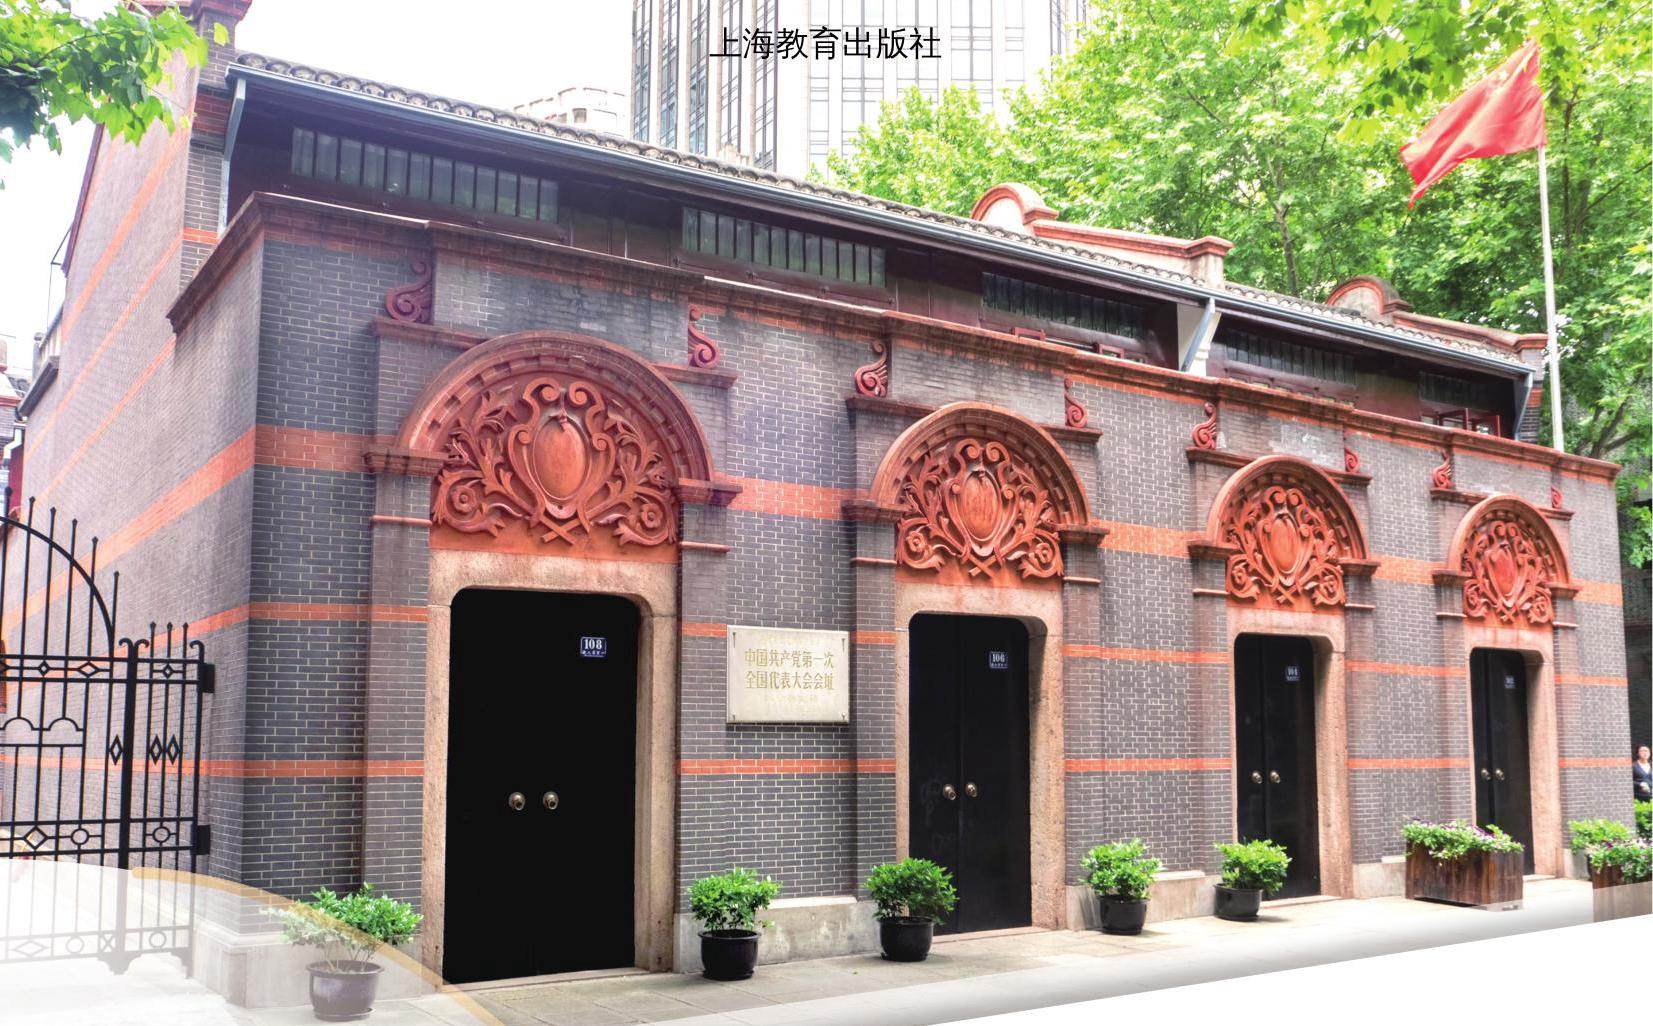
\includegraphics[max width=1.0\textwidth]{images/bo_d7fr3gc91nqc7381iccg_7_1_0_1653_1026_0.jpg}
\end{center}
\hspace*{3em} 

数学语言十分精确, 不容易产生歧义. 集合是现代数学语言的重要组成部分. 使用集合的语言, 可以准确、简洁地表示所要研究的对象, 更好地描述所研究的对象之间的关系.

数学作为很多其他学科的基础和工具, 其内涵及语言都是按照逻辑的方式来组织的. 根据正确的前提, 按照严格的逻辑推理, 总是能够得到正确的结论.

在数学语言的表达方面，有一些公认的特殊约定，努力学习并遵循这些约定，能够更好地在数学领域里与他人开展交流, 对进一步的学习和研究都非常有益.



\section*{1.1 集合初步}

1 集合

\begin{center}
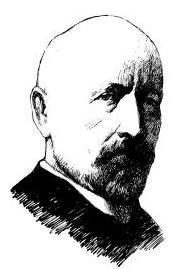
\includegraphics[max width=0.2\textwidth]{images/bo_d7fr3gc91nqc7381iccg_8_263_738_174_269_0.jpg}
\end{center}
\hspace*{3em} 

康托 (G. Cantor, 1845- 1918), 德国数学家, 集合论创始人.

我们经常需要把满足一定要求或具有一定特征的对象放在一起或归为一类. 例如:

(1)申辉中学高一(1)班的全体学生；

(2)所有不大于 100 的自然数；

(3)直线 \(l\) 上的所有点；

(4)不等式 \({2x} + 1 \leq  0\) 的所有解；

(5)太阳系的所有行星.

概括地说, 把一些确定的对象的全体叫做集合 (set), 简称集. 集合通常用大写字母 \(A\text{ 、 }B\text{ 、 }C\cdots \cdots\) 表示.

集合所含的各个对象叫做该集合的元素 (element). 元素通常用小写字母 \(a\text{ 、 }b\text{ 、 }c\cdots \cdots\) 表示.

如果 \(a\) 是集合 \(A\) 的元素，就记作 \(a \in  A\) ，读作“ \(a\) 属于 \(A\) ”； 如果 \(a\) 不是集合 \(A\) 的元素，就记作 \(a \notin  A\) ，读作“ \(a\) 不属于 \(A\) ”. 例如,若 \(A\) 是由数 \(1\text{ 、 }3\text{ 、 }5\text{ 、 }7\text{ 、 }9\) 组成的集合,则 \(1 \in  A,2 \notin  A\) .

集合的元素是确定的. 也就是说, 给定一个集合, 一个对象在不在这个集合中就确定了. 例如, “我国的直辖市”组成一个集合，北京、上海、天津、重庆在这个集合中，而杭州、南京、深圳等城市不在这个集合中.

一些不确定的对象不能组成一个集合. 例如, “我们班里高个子的同学”不能组成一个集合. 因为“高个子”的标准不够明确、 具体, 所以 “我们班里高个子的同学” 是不确定的.

一个给定集合中的各个元素是互不相同的, 即一个元素在同一个集合中是不能重复出现的.

如果两个集合 \(A\) 与 \(B\) 的组成元素完全相同,就称这两个集合相等,记作 \(A = B\) .

\section*{}

\section*{}

元素个数有限的集合称为有限集, 否则就称为无限集.

例 1 判断下列集合是有限集还是无限集, 并说明理由:

(1)6 的正整数倍的全体组成的集合;

(2)600 的正约数的全体组成的集合;

(3)2019 年在上海出生的所有人组成的集合；

(4)给定的一条长度为 1 的线段上的所有点组成的集合.

解(1)6 的正整数倍可表示为 \({6n}\) ，其中 \(n\) 是正整数. 因为正整数有无限个, 所以 6 的正整数倍的全体组成的集合是一个无限集.

(2)600 的正约数一定是小于或等于 600 的正整数，其个数不超过 600 . 所以 600 的正约数的全体组成的集合是一个有限集.

(3)虽然 2019 年出生在上海的人比较多，但总数还是有限的. 所以 2019 年在上海出生的所有人组成的集合是一个有限集.

(4)因为该线段的二等分点、三等分点、四等分点……都是该集合中的元素，所以一条给定的长度为 1 的线段上的所有点组成的集合是一个无限集.

数学中, 常常需要用到数的集合. 数的集合简称数集. 常用的数集可用以下特定的符号来表示，见表 1-1.

表 1-1 常用数集的符号

\begin{center}
\adjustbox{max width=\textwidth}{
\begin{tabular}{|c|c|}
\hline
数集 & 符号 \\
\cline{1-2}
自然数集 & N \\
\cline{1-2}
整数集 & Z \\
\cline{1-2}
有理数集 & Q \\
\cline{1-2}
实数集 & R \\
\cline{1-2}
\hline
\end{tabular}
}
\end{center}

例 2 用符号“ \(\in\) ”或“ \(\notin\) ”填空:

(1)0\_\_\_\_\_N； (2)1\_\_\_\_\_Z；

(3) \(\sqrt{2}\) \_\_\_\_\_ \(\mathbf{Q}\) ； (4) \(- \sqrt{\pi }\) \_\_\_\_\_ \(\mathbf{R}\) .

解 (1) \(0 \in  \mathbf{N}\) . (2) \(1 \in  \mathbf{Z}\) . (3) \(\sqrt{2} \notin  \mathbf{Q}\) . (4) \(- \sqrt{\pi } \in  \mathbf{R}\) .

不含有任何元素的集合称为空集，记作 \(\varnothing\) . 引进空集是有必要的. 例如,方程 \({x}^{2} + 1 = 0\) 没有实数解,我们就说它的实数解组成的集合是空集. 又如, 当两条直线平行时, 它们没有公共点, 就可说这两条直线的公共点组成的集合是空集. 在以后学习交集时, 我们还将进一步体会到引入空集的必要性.





\section*{练习 1.1(1)}

1. 判断下列各组对象能否组成集合. 若能组成集合, 指出是有限集还是无限集; 若不能组成集合, 请说明理由.

(1)上海市现有各区的名称；

(2)末位是 3 的自然数；

(3)比较大的苹果.

2. 用符号“ \(\in\) ”或“ \(\notin\) ”填空:

(1) \(\frac{1}{2}\) \_\_\_\_\_ \(\mathrm{N}\) ； (2)5\_\_\_\_\_ \(\mathrm{Z}\) ；

(3)-2 (4) \(\pi\) \_\_\_\_\_R.

\section*{2 集合的表示方法}

除了用自然语言描述集合，我们还有一些其他方法用来表示集合.

将集合中的元素不重复地一一列举出来并写在大括号内, 这种表示集合的方法叫做列举法. 例如,方程 \({x}^{2} - {3x} + 2 = 0\) 的所有解组成的集合可以表示为 \(\{ 1,2\}\) ,也可以表示为 \(\{ 2,1\}\) . 这是因为在讨论集合时, 不考虑其元素的顺序.

例 3 用列举法表示下列集合:

(1)所有不大于 10 的正整数组成的集合;

(2)方程 \(\left( {x - 1}\right) \left( {x - 2}\right) \left( {x - 3}\right) \left( {x - 4}\right)  = 0\) 的所有解组成的集合;

(3)集合 \(\{ 1,2,3,4\}\) 中任意两个不同元素之和组成的集合.

解 (1) 所有不大于 10 的正整数组成的集合是 \(\{ 1,2,3,4,5\) , \(6,7,8,9,{10}\}\) .

(2)该方程的所有解组成的集合是 \(\{ 1,2,3,4\}\) .

(3)该集合中任意两个不同元素之和组成的集合是 \(\{ 3,4,5,6,7\}\) .

能用列举法表示的集合一般是有限集, 但对于一些有规律的无限集, 在不会引起歧义的前提下, 也可用列举法表示. 例如, 全体正偶数组成的集合可以表示为 \(\{ 2,4,6,\cdots ,{2n},\cdots \}\) .

集合还有另外一种表示方法.

\section*{}

在大括号内先写出这个集合中元素的一个记号, 再画一条竖线, 并在竖线的右边写上集合中所有元素具有的共同特征, 即

\[
A = \{ x \mid  x\text{ 满足性质 }p\} \text{ . }
\]

这种表示集合的方法叫做描述法. 例如,方程 \({x}^{2} - {3x} + 2 = 0\) 的所有解组成的集合可以表示为 \(\left\{  {x \mid  {x}^{2} - {3x} + 2 = 0}\right\}\) . 又如,函数 \(y = x\) 图像上的所有点组成的集合可以表示为 \(\{ \left( {x,y}\right)  \mid  y = x\}\) .

例 4 选择适当的方法表示下列集合:

(1)大于 0 且小于 10 的全体偶数组成的集合 \(A\) ；

(2)被 3 除余 2 的所有自然数组成的集合 \(B\) ；

(3)直角坐标平面上由第二象限与第四象限中的所有点组成的集合 \(C\) .

解 (1) 用列举法: \(A = \{ 2,4,6,8\}\) .

(2)用描述法: \(B = \{ n \mid  n = {3k} + 2,k \in  \mathbf{N}\}\) .

(3)因为第二象限中所有点 \(\left( {x,y}\right)\) 具有的特征是 \(x < 0\) 且 \(y > 0\) ,而第四象限中所有点具有的特征是 \(x > 0\) 且 \(y < 0\) ,所以第二象限与第四象限中所有点具有的特征可统一地写为 \({xy} < 0\) ,于是可用描述法表示该集合:

\[
C = \{ \left( {x,y}\right)  \mid  {xy} < 0\} .
\]

数学中, 常常需要表示满足一些不等式的全体实数所组成的集合. 为了方便起见, 我们引入区间 (interval) 的概念.

当 \(a\text{ 、 }b \in  \mathbf{R}\) 且 \(a < b\) 时,规定:

满足不等式 \(a \leq  x \leq  b\) 的全体实数 \(x\) 组成的集合称为一个闭区间,记作 \(\left\lbrack  {a,b}\right\rbrack\) .

满足不等式 \(a < x < b\) 的全体实数 \(x\) 组成的集合称为一个开区间,记作 \(\left( {a,b}\right)\) .

闭区间与开区间在数轴上的表示，如图 1-1-1 所示.

\begin{center}
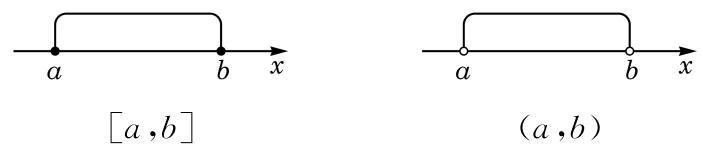
\includegraphics[max width=0.6\textwidth]{images/bo_d7fr3gc91nqc7381iccg_11_272_1832_703_152_0.jpg}
\end{center}
\hspace*{3em} 

图 1-1-1

满足不等式 \(a \leq  x < b\) 或 \(a < x \leq  b\) 的全体实数 \(x\) 所组成的集合称为一个半开半闭区间,分别记作 \(\left\lbrack  {a,b)\text{ 或 }(a,b}\right\rbrack\) .



\HRule

“集合中所有元素具有的共同特征”是指:

(1)在该集合中的元素都具有这个特征;

(2)不在该集合中的元素不具有这个特征.

\HRule

\section*{}

半开半闭区间在数轴上的表示, 如图 1-1-2 所示.

\begin{center}
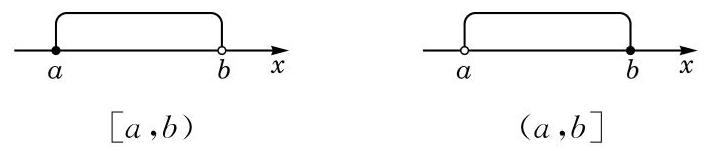
\includegraphics[max width=0.6\textwidth]{images/bo_d7fr3gc91nqc7381iccg_12_669_293_705_151_0.jpg}
\end{center}
\hspace*{3em} 

图 1-1-2

这里的实数 \(a\text{ 、 }b\) 统称为这些区间的端点.

此外,满足不等式 \(x \geq  a,x > a,x \leq  b\) 或 \(x < b\) 的全体实数 \(x\) 所组成的集合可分别用区间表示为 \(\lbrack a, + \infty ),\left( {a, + \infty }\right)\) , \(( - \infty ,b\rbrack\) 或 \(\left( {-\infty ,b}\right)\) . Q

\HRule

符号“ \(\infty\) ”读作“无穷大”.

\HRule

实数集 \(\mathbf{R}\) 可用区间表示为 \(\left( {-\infty , + \infty }\right)\) .

? 例 5 用区间表示下列集合:

\HRule

结合例题, 试比较分别用自然语言、 列举法、描述法和区间表示集合时, 其各自的特点和适用对象.

\HRule

(1) \(\{ x \mid  1 \leq  x < 2\}\) ；

(2)不等式 \({2x} \leq  6\) 的所有解组成的集合.

解 (1) 该集合可用区间 \(\left\lbrack  {1,2}\right)\) 表示.

(2)因为不等式 \({2x} \leq  6\) 的解是 \(x \leq  3\) ，所以它的所有解组成的集合是 \(( - \infty ,3\rbrack\) .

\section*{练习 1.1(2)}

1. 用列举法表示下列集合:

(1)能整除 10 的所有正整数组成的集合;

(2)绝对值小于 4 的所有整数组成的集合.

2. 用描述法表示下列集合:

(1)全体偶数组成的集合;

(2)平面直角坐标系中 \(x\) 轴上所有点组成的集合.

3. 用区间表示下列集合:

(1) \(\{ x \mid   - 1 < x \leq  5\}\) ；

(2)不等式 \(- {2x} > 6\) 的所有解组成的集合.

\section*{3 集合之间的关系}

考察以下四组集合:

(1)C 是申辉中学高一(1)班的全体学生组成的集合，D 是



申辉中学全体学生组成的集合;

(2)C是一平面上所有矩形组成的集合， \(D\) 是该平面上所有平行四边形组成的集合;

(3) \(C = \{ 2,3\} ,D = \left\{  {x \mid  {x}^{2} - {5x} + 6 = 0}\right\}\) ;

(4) \(C = \{ x \mid  x = {2k} + 1,k \in  \mathbf{Z}\} ,D = \{ x \mid  x\) 是奇数 \(\}\) .

容易发现,在上述每组集合中,集合 \(C\) 中的每个元素都属于集合 \(D\) . 两个集合之间的这种关系是十分常见的.

定义 对于两个集合 \(A\) 与 \(B\) ,如果集合 \(A\) 的每个元素都是集合 \(B\) 的元素，那么集合 \(A\) 叫做集合 \(B\) 的子集 (subset)，记作 \(A \subseteq  B\) (或 \(B \supseteq  A\) ),读作“ \(A\) 包含于 \(B\) ”(或“ \(B\) 包含 \(A\) ”).

对任何集合 \(A\) ,规定

\[
\varnothing  \subseteq  A\text{ . }
\]

\begin{center}
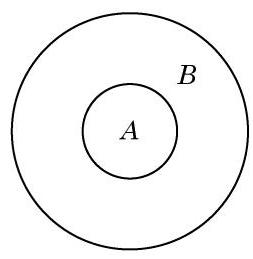
\includegraphics[max width=0.2\textwidth]{images/bo_d7fr3gc91nqc7381iccg_13_1174_960_253_259_0.jpg}
\end{center}
\hspace*{3em} 

图 1-1-3

我们常用维恩图 (Venn diagram) 来直观表示集合以及集合之间的关系. 图 1-1-3 是 \(A \subseteq  B\) 的维恩图.

上述四组集合中的每组都有 \(C \subseteq  D\) . 但是,第 (1)(2)组与第 (3)(4)组是有区别的. 在第(1)(2)组中，集合 \(D\) 中有些元素不属于集合 \(C\) ,即 \(D\) 不是 \(C\) 的子集; 而在第(3)(4)组中，集合 \(D\) 中的每个元素都属于集合 \(C\) ,即 \(D \subseteq  C\) .

对于集合之间的包含关系，我们有下列结论:

(1) \(A \subseteq  A\) ； Q

\HRule

集合关系中的“若 \(A \subseteq  B\) 且 \(B \subseteq  A\) ,则 \(A \; = {B}^{n}\) 与实数大小关系中“若 \(a \leq  b\) 且 \(b \leq  a\) , 则 \(a = b\) ” 类似.

\HRule

(2)若 \(A \subseteq  B\) 且 \(B \subseteq  A\) ,则 \(A = B\) ；

(3)传递性:若 \(A \subseteq  B\) 且 \(B \subseteq  C\) ，则 \(A \subseteq  C\) .

由此,对第 (3) (4) 组集合, \(C = D\) 成立; 而对第 (1) (2) 组集合, \(C = D\) 不成立. 为此,我们引入真子集的概念.

定义 对于两个集合 \(A\) 与 \(B\) ,如果 \(A \subseteq  B\) ,且 \(B\) 中至少有一个元素不属于 \(A\) (即 \(B\) 不是 \(A\) 的子集),那么称集合 \(A\) 是集合 \(B\) 的真子集 (proper subset),记作 \(A \subset  B\) (或 \(B \supset  A\) ),读作“ \(A\) 真包含于 \(B\) ”(或“ \(B\) 真包含 \(A\) ”).

对第(1)(2)组集合， \(C \subset  D\) 成立.

对于常用的数集, 我们有如下的包含关系:

\[
\mathrm{N} \subset  \mathrm{Z} \subset  \mathrm{Q} \subset  \mathrm{R}\text{ . }
\]





例 6 确定 \(x\) 与 \(y\) ,使得集合 \(\{ {2x},x + y\}  = \{ 4,8\}\) .

解 由集合相等的定义, 可知

\[
\left\{  {\begin{array}{l} {2x} = 4, \\  x + y = 8 \end{array}\text{ 或 }\left\{  \begin{array}{l} {2x} = 8, \\  x + y = 4. \end{array}\right. }\right.
\]

?

\HRule

此处为什么有两种情况?

\HRule

分别解得 \(\left\{  \begin{array}{l} x = 2, \\  y = 6 \end{array}\right.\) 或 \(\left\{  \begin{array}{l} x = 4, \\  y = 0. \end{array}\right.\)

例 7 确定下列每组中两个集合之间的关系:

(1) \(A = \{ n \mid  n\) 是 12 的正约数 \(\} ,B = \{ 1,2,3,6\}\) ;

(2) \(C = \{ n \mid  n = {{3k} + 1},k \in  \mathbf{N}\} ,D = \{ n \mid  n = {{3m} - 2},m \in  \mathbf{N}\}\) .

解 (1) 因为 \(A = \{ 1,2,3,4,6,{12}\}\) ,所以 \(B \subset  A\) .

(2)因为当 \(k \in  \mathbf{N}\) 时， \(C\) 中的元素 \(n = {{3k} + 1} = 3\left( {k + 1}\right)  - 2\) 必定属于 \(D\) ,所以 \(C \subseteq  D\) .

又因为 \(- 2 \in  D\) ,而 \(- 2 \notin  C\) ,所以 \(C \subset  D\) .

例 8 写出集合 \(\{ a,b,c\}\) 的所有子集,并指出哪些是真子集.

解 可以按照子集的元素个数分类:

不含任何元素的子集 1 个: 空集 \(\varnothing\) ;

含 1 个元素的子集 3 个: \(\{ a\} ,\{ b\} ,\{ c\}\) ;

含 2 个元素的子集 3 个: \(\{ a,b\} ,\{ a,c\} ,\{ b,c\}\) ;

含 3 个元素的子集 1 个: \(\{ a,b,c\}\) .

除集合 \(\{ a,b,c\}\) 本身外,其余 7 个都是真子集.

\section*{练习 1.1(3)}

1. 判断下列说法是否正确, 并简要说明理由:

(1)若 \(a \in  A\) 且 \(A \subseteq  B\) ，则 \(a \in  B\) ；

(2)若 \(A \subseteq  B\) 且 \(A \subseteq  C\) ，则 \(B = C\) ；

(3)若 \(A \subset  B\) 且 \(B \subseteq  C\) ，则 \(A \subset  C\) .

2. 用符号“ \(\neg\) ”“=”或“⊂”填空:

(1) \(\{ a\}\)

(2) \(\{ a,b,c\}\) \_\_\_\_\_ \(\{ a,c\}\) ；

(3) \(\{ 1,2\}\) \_\_\_\_\_ \(\{ x \mid  {x}^{2} - {3x} + 2 = 0\}\) .

3. 写出所有满足 \(\{ a\}  \subset  M \subset  \{ a,b,c,d\}\) 的集合 \(M\) .

\section*{4 集合的运算}

先看一个校园生活的例子. 申辉中学高一年级的学生报名参加数学建模社与理学社. 这样, 除该校高一年级的全体学生组成的集合 \(U\) 外,还有参加数学建模社的学生组成的集合 \(A\) ,参加理学社的学生组成的集合 \(B\) ,两个社都参加的学生组成的集合 \(C\) ,两个社中至少参加一个的学生组成的集合 \(D\) ,还有未参加数学建模社的学生组成的集合 \(E\) ,等等.

可以看到,集合 \(A\text{ 、 }B\text{ 、 }C\text{ 、 }D\text{ 、 }E\) 等都是集合 \(U\) 的子集, 集合 \(C\) 是由集合 \(A\) 与 \(B\) 的公共元素组成的,集合 \(D\) 是由集合 \(A\) 与 \(B\) 的所有元素组成的,集合 \(E\) 是由集合 \(U\) 中去掉 \(A\) 中的元素后剩下的元素组成的.

本节我们要从已知的集合出发，通过“交”“并”“补”的运算得到新的集合.

首先, 我们可以对任意两个集合取公共元素, 从而得到一个新的集合.

定义 由既属于集合 \(A\) 又属于集合 \(B\) 的所有元素组成的集合,叫做集合 \(A\) 与 \(B\) 的交集(intersection),记作 \(A \cap  B\) (读作“A 交 \(B\) ”),即

\[
A \cap  B = \{ x \mid  x \in  A\text{ 且 }x \in  B\} .
\]

可以用维恩图直观地反映 \(A \cap  B\) 的几种不同情况,如图 1-1-4 所示.

\begin{center}
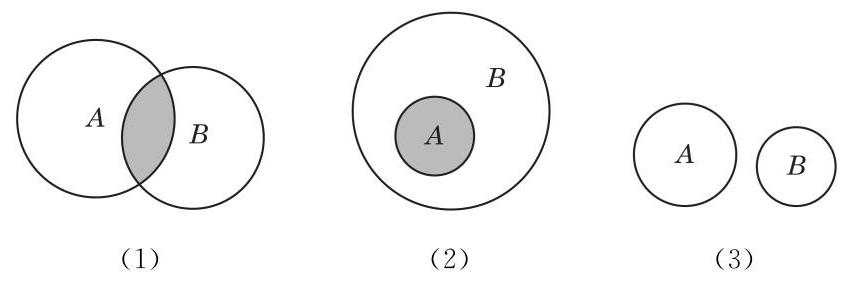
\includegraphics[max width=0.7\textwidth]{images/bo_d7fr3gc91nqc7381iccg_15_203_1592_847_281_0.jpg}
\end{center}
\hspace*{3em} 

图 1-1-4

图 1-1-4(1)表示集合 \(A\) 与 \(B\) 既有公共元素又都有非公共元素的情况,此时阴影部分 \(A \cap  B\) 既是 \(A\) 的真子集又是 \(B\) 的真子集; 图 1-1-4(2) 表示集合 \(A\) 是 \(B\) 的子集的情况,此时 \(A \cap  B = A\) ; 图 1-1-4(3)表示集合 \(A\) 与 \(B\) 没有公共元素的情况,

此时 \(A \cap  B = \varnothing\) .

\HRule

当集合 \(U\text{ 、 }A\text{ 、 }B\) 确定时, 如何确定集合 \(C\text{ 、 }D\text{ 、 }E\) 呢?

对照图 1-1-4 的三种情况, 请各举一实例.

\HRule

例 9 已知集合

\[
A = \{ \left( {x,y}\right)  \mid  {2x} + y = 5\} ,B = \{ \left( {x,y}\right)  \mid  {3x} + {2y} = 8\} .
\]

求 \(A \cap  B\) .

解 由题意, \(\left( {x,y}\right)  \in  A \cap  B\) 表示 \(\left( {x,y}\right)\) 既属于 \(A\) 又属于 \(B\) ,即 \(\left( {x,y}\right)\) 是方程组

\[
\left\{  \begin{array}{l} {2x} + y = 5, \\  {3x} + {2y} = 8 \end{array}\right.
\]

的解,所以 \(x = 2,y = 1\) . 于是, \(A \cap  B = \{ \left( {2,1}\right) \}\) .

其次, 我们可以把两个已知集合的所有元素放在一起组成一个新的集合.

定义 由所有属于集合 \(A\) 或属于集合 \(B\) 的元素所组成的集合,叫做集合 \(A\) 与 \(B\) 的并集 (union),记作 \(A \cup  B\) (读作“ \(A\) 并 B”), 即

\[
A \cup  B = \{ x \mid  x \in  A\text{ 或 }x \in  B\} .
\]

可以用维恩图直观地反映 \(A \cup  B\) 的几种不同情况,如图 1-1-5所示,其中阴影部分表示 \(A \cup  B\) .

?

\begin{center}
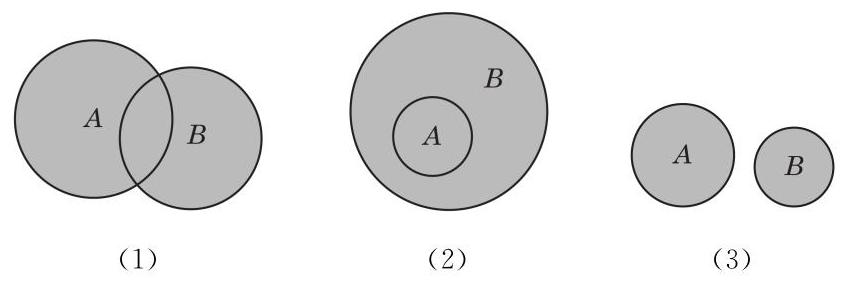
\includegraphics[max width=0.7\textwidth]{images/bo_d7fr3gc91nqc7381iccg_16_603_1332_844_281_0.jpg}
\end{center}
\hspace*{3em} 

图 1-1-5

图 1-1-5(1)表示集合 \(A\) 与 \(B\) 既有公共元素又都有非公共元素的情况,此时 \(A\) 和 \(B\) 都是 \(A \cup  B\) 的真子集; 图 1-1-5(2) 表示集合 \(A\) 是 \(B\) 的子集的情况,此时 \(A \cup  B = B\) ; 图 1-1-5(3) 表示集合 \(A\) 与 \(B\) 没有公共元素的情况.

例 10 已知集合

\[
A = \left( {-2,2}\right) ,B = \left( {-3, - 1}\right)  \cup  \left( {1, + \infty }\right) .
\]

求 \(A \cap  B\) 及 \(A \cup  B\) .

解 在数轴上标出集合 \(A\) 与 \(B\) ,如图 1-1-6 所示.

\section*{}

\HRule

例 9 中, \(A \cap  B\) 表示二元一次方程组的所有解组成的集合. 它可以理解为两个一次函数 \(y =  - {2x} + 5\) 与 \(y =  - \frac{3}{2}x + 4\) 的图像的交点组成的集合.

对照图 1-1-5 的三种情况, 请各举一实例.

\HRule

\begin{center}
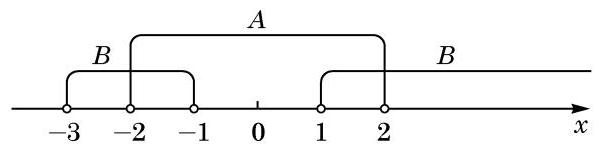
\includegraphics[max width=0.5\textwidth]{images/bo_d7fr3gc91nqc7381iccg_17_326_264_598_152_0.jpg}
\end{center}
\hspace*{3em} 

图 1-1-6

于是 \(A \cap  B = \left( {-2, - 1}\right)  \cup  \left( {1,2}\right) ,A \cup  B = \left( {-3, + \infty }\right)\) .

例 11 已知集合 \(A = \{ 1,2\}\) ，求所有满足 \(A \cup  B = \{ 1,2,3\}\) 的集合 \(B\) .

解 因为 \(B \subseteq  A \cup  B = \{ 1,2,3\}\) ,所以 \(B\) 的元素只能在 1、2、3 中取. 为了使得 \(A \cup  B\) 中有 3,3 必须是 \(B\) 的一个元素. 至于 1、2 是否为 \(B\) 的元素，不会影响 \(A \cup  B\) 的结果.

因此，满足条件的集合 \(B\) 一共有 4 个: \(\{ 3\} ,\{ 1,3\}\) ， \(\{ 2,3\} ,\{ 1,2,3\}\) .

最后, 我们介绍全集与补集.

在数学研究中, 所研究的对象往往是某个确定集合的一个子集或元素. 例如, 求方程的实数解时, 所有解组成的集合一定是实数集 \(\mathbf{R}\) 的一个子集; 求三角形的内角的大小时,如果以度 \(\left( {}^{ \circ  }\right)\) 为单位,那么角的度数一定是开区间 \(\left( {0,{180}}\right)\) 中的一个元素; 等等. 这个确定的集合称为全集 (universal set),常用符号 \(U\) 表示. 它含有我们所要研究问题的全部可能的元素.

定义 设 \(U\) 为全集, \(A\) 是 \(U\) 的子集. 由 \(U\) 中所有不属于 \(A\) 的元素组成的集合称为集合 \(A\) 在全集 \(U\) 中的补集 (complementary set),记作 \(\bar{A}\) (读作“ \(A\) 补”),即

\[
\bar{A} = \{ x \mid  x \in  U\text{ 且 }x \notin  A\} .
\]

有时为了强调全集 \(U\) ,集合 \(A\) 在全集 \(U\) 中的补集 \(\bar{A}\) 也可以记作 \({\complement }_{U}A\) .

当全集为实数集 \(\mathbf{R}\) 时,有理数集 \(\mathbf{Q}\) 的补集 \(\overline{\mathbf{Q}}\) 就是全体无理数组成的集合.

可以用维恩图直观地反映 \(\bar{A}\) ,如图 1-1-7,其中阴影部分表示集合 \(A\) 在全集 \(U\) 中的补集 \(\bar{A}\) .

\begin{center}
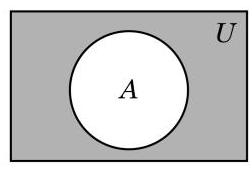
\includegraphics[max width=0.2\textwidth]{images/bo_d7fr3gc91nqc7381iccg_17_1174_1818_252_169_0.jpg}
\end{center}
\hspace*{3em} 

图 1-1-7

例 12 设全集 \(U = \{ a,b,c,d,e\}\) ,集合 \(A = \{ a,b,c\}\) , 集合 \(B = \{ c,d\}\) . 分别求: \(\overline{A \cup  B},\bar{A} \cap  \bar{B},\overline{A \cap  B}\) 及 \(\bar{A} \cup  \bar{B}\) .

解 由条件, 可得





\[
A \cup  B = \{ a,b,c,d\} ,\bar{A} = \{ d,e\} ,\bar{B} = \{ a,b,e\} .
\]

所以

\[
\overline{A \cup  B} = \{ e\} ,\bar{A} \cap  \bar{B} = \{ e\} .
\]

而 \(A \cap  B = \{ c\}\) ,所以

\[
\overline{A \cap  B} = \{ a,b,d,e\} ,\overline{A} \cup  \overline{B} = \{ a,b,d,e\} .
\]

\section*{练习 1.1(4)}

1. 设 \(A\) 为全集 \(U\) 的任一子集,则

(1) \(\overline{\overline{A = }}\) \_\_\_\_\_；( \(\overline{\overline{A = }}\) 表示 \(A\) 的补集 \(\overline{A\text{ 的 }}\) 的补集.

(2) \(A \cap  \overline{A} =\) \_\_\_\_\_；

(3) \(A \cup  \overline{A} =\) \_\_\_\_\_.

2. 已知全集为 \(\mathbf{R}\) ,集合 \(A = \{ x \mid   - 2 < x \leq  1\}\) . 求 \(\overline{A}\) .

3. 已知集合 \(A = \{ 1,2,3,4,5\} ,B = \{ 2,4,6,8\} ,C = \{ 3,4,5,6\}\) . 求:

(1) \(\left( {A \cap  B}\right)  \cup  C,\left( {A \cup  C}\right)  \cap  \left( {B \cup  C}\right)\) ；

(2) \(\left( {A \cup  B}\right)  \cap  C,\left( {A \cap  C}\right)  \cup  \left( {B \cap  C}\right)\) .

\section*{习题 1.1}

\section*{A 组}

1. 用列举法表示下列集合:

(1)10 以内的所有素数组成的集合;

(2) \(\left\{  {y\left| {\;y = x - 1}\right. ,0 \leq  x \leq  3,x \in  \mathbf{Z}}\right\}\) .

2. 用描述法表示下列集合:

(1) 被 3 除余 1 的所有自然数组成的集合;

(2)比 1 大又比 10 小的所有实数组成的集合;

(3)平面直角坐标系中坐标轴上所有点组成的集合.

3. 集合 \(\{ \left( {x,y}\right)  \mid  {xy} > 0,x\text{ 、 }y\) 为实数 \(\}\) 是指 ( )

A. 第一象限内的所有点组成的集合;

B. 第三象限内的所有点组成的集合;

C. 第一象限和第三象限内的所有点组成的集合;

D. 不在第二象限也不在第四象限内的所有点组成的集合.



\section*{}

4. 用符号“ \(\subset\) ”“=”或“ \(\supset\) ”连接集合 \(A\) 与 \(B\) :

(1) \(A = \left\{  {x \mid  {x}^{2} - {2x} + 1 = 0}\right\}  ,B = \left\{  {x \mid  {x}^{2} - 1 = 0}\right\}\) ；

(2) \(A = \{ 1,2,4,8\} ,B = \{ x \mid  x\) 是 8 的正约数 \(\}\) .

5. 已知集合 \(A = \{ 1\} ,B = \left\{  {x \mid  {x}^{2} - {3x} + a = 0}\right\}\) . 是否存在实数 \(a\) ，使得 \(A \subset  B\) ？若存在,求 \(a\) 的值; 若不存在,说明理由.

6. 已知集合 \(A = \{ x,y\} ,B = \left\{  {{2x},2{x}^{2}}\right\}\) ，且 \(A = B\) . 求集合 \(A.\)

7. 已知集合 \(A = \{ x \mid  x \leq  7\} ,B = \{ x \mid  x < 2\} ,C = \{ x \mid  x > 5\}\) . 求: \(A \cap  B,A \cap  C\) , \(A \cap  \left( {B \cap  C}\right)\) .

8. 已知集合 \(A = \{ \left( {x,y}\right)  \mid  y =  - x + 1\} ,B = \left\{  {\left( {x,y}\right)  \mid  y = {x}^{2} - 1}\right\}\) . 求 \(A \cap  B\) .

9. 已知全集 \(U = \mathbf{R}\) ，集合 \(A = \{ x \mid  4 - x > {2x} + 1\}\) . 求 \(\overline{A}\) .

B 组

1. 已知集合 \(A = \left\{  {2,{\left( a + 1\right) }^{2},{a}^{2} + {3a} + 3}\right\}\) ，且 \(1 \in  A\) . 求实数 \(a\) 的值.

2. 已知集合 \(A = \{ x \mid  x = {{2n} + 1},n \in  \mathbf{Z}\} ,B = \{ x \mid  x = {{4n} - 1},n \in  \mathbf{Z}\}\) . 判断集合 \(A\) 与 \(B\) 的包含关系,并证明你的结论.

3. 设 \(a\) 是实数,集合 \(M = \left\{  {x \mid  {x}^{2} + x - 6 = 0}\right\}  ,N = \{ y \mid  {ay} + 2 = 0\}\) . 是否存在 \(a\) ,使得 \(N \subset  M\) ? 若存在,求这些 \(a\) 的值; 若不存在,说明理由.

4. 已知集合 \(A = \{ 1,4,x\} ,B = \left\{  {1,{x}^{2}}\right\}\) ，且 \(A \cup  B = A\) . 求 \(x\) 的值及集合 \(A\) 、 \(B\) .

\section*{1.2 常用逻辑用语}

\section*{1 命题}

在初中时已经知道, 用自然语言、符号或式子表达, 且可以判断其真假的语句叫做命题 (proposition)。命题通常用陈述句表述. 其含义判断为真的命题叫做真命题, 判断为假的命题叫做假命题. 例如, “ 4 能被 2 整除”是真命题， “ 3 能被 2 整除”是假命题.

例 1 下列语句哪些是命题？如果是命题，那么它们是真命题还是假命题？为什么？

(1)个位数字是 5 的自然数能被 5 整除；

(2)凡直角三角形都相似；

(3)请起立；

(4)若两个角互为补角，则这两个角不相等；

(5)若两个三角形的三组对应边相等，则这两个三角形全等;

(6)你是高一学生吗？

(7) \(x > 3\) .

解 语句(3)(6)(7)不是命题；语句(1)(2)(4)(5)是命题，其中语句(1)(5)是真命题，语句(2)(4)是假命题.

(1)这是一个真命题. 因为个位数字是 5 的自然数可写成 \({10k} + 5\) 的形式 \(\left( {k \in  \mathbf{N}}\right)\) ,而 \({10k} + 5 = 5\left( {{2k} + 1}\right)\) ,它总能被 5 整除, 所以个位数字是 5 的自然数能被 5 整除.

(2)因为三个角分别为 \({90}^{ \circ  }\) 、 \({45}^{ \circ  }\) 、 \({45}^{ \circ  }\) 的直角三角形与三个角分别为 \({90}^{ \circ  }\) 、 \({60}^{ \circ  }\) 、 \({30}^{ \circ  }\) 的直角三角形是不相似的，所以“凡直角三角形都相似”是一个假命题.

(3)“请起立”无法判定真假，它不是一个命题.

(4)取一个角为 \({90}^{ \circ  }\) ，另一个角也为 \({90}^{ \circ  }\) ，它们是互补的，同

\section*{}

时它们也是相等的, 所以 “若两个角互为补角, 则这两个角不相等”是一个假命题.

(5) 这是一个真命题, 它是两个三角形全等的一个判定定理.

(6)因为“你是高一学生吗？”不是陈述句，无法判断其真假， 所以它不是命题.

(7)虽然“ \(x > 3\) ”是陈述句，但是它包含一个可变的对象 \(x\) ， 无法判断其真假，因此它不是命题. 当 \(x\) 被赋予不同的值时，它就成为不同的命题. 例如,当 \(x = 4\) 时,“ \(x > 3\) ” 是真命题；当 \(x = 1\) 时,“ \(x > 3\) ”是假命题.

例 1 中命题( 4 )与( 5 )具有“若 \(\alpha\) ，则 \(\beta\) ”的形式. 在保持含义不变的前提下，例 1 中命题( 1 )与( 2 )也可改写为这种形式:

若一个自然数的个位数字是 5 ，则这个自然数能被 5 整除；

若两个三角形都是直角三角形, 则它们相似.

在形如

“若 \(\alpha\) ,则 \(\beta\) ”

的命题中,陈述句 \(\alpha\) 称为条件, \(\beta\) 称为结论.

命题“若 \(\alpha\) ,则 \(\beta\) ”是真命题,是指所有满足条件 \(\alpha\) 的对象都满足结论 \(\beta\) . 用集合的语言描述即

\(\{ x \mid  x\) 满足 \(\alpha \}  \subseteq  \{ x \mid  x\) 满足 \(\beta \}\) .

所以, 要确定这类命题是真命题, 就必须给出其证明, 如例 1 中的(1)与(5).

命题“若 \(\alpha\) ,则 \(\beta\) ”是假命题,是指存在满足条件 \(\alpha\) 的对象, 它不满足结论 \(\beta\) . 所以,要确定这类命题是假命题,可用处理例 1 中( 2 )与( 4 )的方法，举一个满足条件 \(\alpha\) 而不满足结论 \(\beta\) 的例子就可以了.

定义 如果命题“若 \(\alpha\) ,则 \(\beta\) ”是真命题,那么就称 \(\alpha\) 推出 \(\beta\) , 记作 \(\alpha  \Rightarrow  \beta\) (或 \(\beta  \Leftarrow  \alpha\) ).

因为子集关系满足传递性, 所以推出关系也满足传递性:

若 \(\alpha  \Rightarrow  \beta\) 且 \(\beta  \Rightarrow  \gamma\) ,则 \(\alpha  \Rightarrow  \gamma\) .

它是逻辑推理的基础.

例 2 将下列命题改写成“若 \(\alpha\) ，则 \(\beta\) ”的形式，并判断 “ \(\alpha  \Rightarrow  \beta\) ” 是否成立.



\HRule

“若 \(\alpha\) ,则 \(\beta\) ”形式的命题也可写为“如果 \(\alpha\) ,那么 \(\beta\) ”的形式.

这种方法在数学上称为举反例.

\HRule

\section*{}

(1)等腰三角形的两底角相等;

(2)凡是素数都是奇数；

(3)对顶角相等.

解(1)若一个三角形是等腰三角形，则它的两个底角相等. 这是一个真命题. 所以，“ \(\alpha  \Rightarrow  \beta\) ”成立.

(2)若 \(n\) 是素数，则 \(n\) 是奇数. 这是一个假命题，因为 2 是素数,但它是偶数. 所以,“ \(\alpha  \Rightarrow  \beta\) ”不成立.

(3)若两个角是对顶角，则这两个角相等. 这是一个真命题. 所以，“ \(\alpha  \Rightarrow  \beta\) ”成立.

\section*{练习 1.2(1)}

1. 举几个生活中的命题的例子, 并判断其真假.

2. 判断下列命题的真假, 并说明理由:

(1)所有偶数都不是素数；

(2) \(\{ 1\}\) 是 \(\{ 0,1,2\}\) 的真子集；

(3)0 是 \(\{ 0,1,2\}\) 的真子集；

(4)如果集合 \(A\) 是集合 \(B\) 的子集，那么 \(B\) 不是 \(A\) 的子集.

3. 用“ \(\Rightarrow\) ”表示下列陈述句 \(\alpha\) 与 \(\beta\) 之间的推出关系:

(1) \(\alpha  : {\bigtriangleup {ABC}}\) 是等边三角形， \(\beta\) : \({\bigtriangleup {ABC}}\) 是轴对称图形；

(2) \(\alpha  : {x}^{2} = 4,\beta  : x = 2\) .

\section*{2 充分条件与必要条件}

先看一个例子:我们要培养的是德智体美劳全面发展的社会主义建设者和接班人. 显然, 对于这样“全面发展”的学生来说, 其学习成绩一定是好的; 反过来, 学习成绩好的学生不一定是 “全面发展”的，因为可能其他方面不是很好. 也就是说，“学习成绩好” 对于“全面发展”是不可缺少的，但只有“学习成绩好”还不够.

定义 对于两个陈述句 \(\alpha\) 与 \(\beta\) ,如果 \(\alpha  \Rightarrow  \beta\) ,就称 \(\alpha\) 是 \(\beta\) 的充分条件 (sufficient condition),亦称 \(\beta\) 是 \(\alpha\) 的必要条件 (necessary condition). Q

\HRule

该定义中,“充分”二字说明 “ \(\alpha\) 成立时， \(\beta\) 一定成立”；而 “必要”二字说明“β不成立时, \(\alpha\) 一定不成立”.

\HRule

由例 2 知道, “一个三角形是等腰三角形”是 “一个三角形有两个角相等”的充分条件，“两个角相等”是“两个角是对顶角”的



必要条件, 而“一个数是素数”不是“一个数是奇数”的充分条件.

例 3 判断下列各组中的 \(\alpha\) 分别是 \(\beta\) 的什么条件,并说明理由.

(1) \(\alpha\) :四边形 \({ABCD}\) 是正方形， \(\beta\) :四边形 \({ABCD}\) 的四个内角都是直角;

(2) \(\alpha  : {x}^{2}\) 是有理数， \(\beta  : x\) 是有理数.

解(1)因为正方形的四个内角都是直角，所以命题“若 \(\alpha\) ， 则 \(\beta\) ”是真命题， \(\alpha\) 是 \(\beta\) 的充分条件.

反之, 因为四个内角都是直角的四边形也可以是长宽不相等的矩形,所以命题“若 \(\beta\) ,则 \(\alpha\) ”是假命题, \(\alpha\) 不是 \(\beta\) 的必要条件.

(2)因为有理数 \(\frac{r}{s}\left( {r\text{ 、 }s \in  \mathbf{Z}}\right)\) 的平方 \(\frac{{r}^{2}}{{s}^{2}}\) 必是一个有理数， 所以“若 \(\beta\) ,则 \(\alpha\) ”是真命题, \(\alpha\) 是 \(\beta\) 的必要条件.

反之,因为 \({\left( \sqrt{2}\right) }^{2} = 2\) 是有理数,但 \(\sqrt{2}\) 是无理数,所以“若 \(\alpha\) ,则 \(\beta\) ”是假命题, \(\alpha\) 不是 \(\beta\) 的充分条件.

定义 对于两个陈述句 \(\alpha\) 与 \(\beta\) ,如果既有 \(\alpha  \Rightarrow  \beta\) ,又有 \(\beta  \Rightarrow  \alpha\) , 就称 \(\alpha\) 是 \(\beta\) 的充分必要条件,简称充要条件,记作 \(\alpha  \Leftrightarrow  \beta\) ,读作 “ \(\alpha\) 与 \(\beta\) 等价”或“ \(\alpha\) 成立当且仅当 \(\beta\) 成立”.

例如, “三角形的两个内角相等”是 “三角形的两条边相等” 的充要条件; “实数 \(x\text{ 、 }y\) 满足 \(\left| x\right|  = \left| y\right|\) ” 是 “实数 \(x\text{ 、 }y\) 满足 \(\left( {x + y}\right) \left( {x - y}\right)  = 0\) ” 的充要条件.

例 4 已知 \(m\) 是实数，集合

\[
M = \{ 2,3,m + 6\} ,N = \{ 0,7\} .
\]

求证:“ \(m = 1\) ” 是 “ \(M \cap  N = \{ 7\}\) ” 的充要条件.

证明 先证充分性 (即证 \(m = 1 \Rightarrow  M \cap  N = \{ 7\}\) ). 当 \(m = 1\) 时, \(M = \{ 2,3,7\}\) . 又因为 \(N = \{ 0,7\}\) ,所以 \(M \cap  N = \{ 7\}\) .

再证必要性 (即证 \(M \cap  N = \{ 7\}  \Rightarrow  m = 1\) ). 当 \(M \cap  N = \{ 7\}\) 时, 由 \(7 \in  M\) ,得 \(m + 6 = 7\) ,因此 \(m = 1\) .

综上所述，“ \(m = 1\) ”是“ \(M \cap  N = \{ 7\}\) ”的充要条件.

\section*{练习 1.2(2)}

1. 已知 \(\alpha\) : 四边形 \({ABCD}\) 的两组对边分别平行, \(\beta\) : 四边形 \({ABCD}\) 为矩形, \(\gamma\) : 四边

\HRule

下一小节将给出 \(\sqrt{2}\) 是无理数的证明.

\HRule

\section*{}

集合与逻辑形 ABCD 的两组对边分别相等. 用 “充分非必要”“必要非充分” “充要”或 “既非充分又非必要”填空:

(1) \(\alpha\) 是 \(\beta\) 的\_\_\_\_\_条件；

(2) \(\beta\) 是 \(\gamma\) 的\_\_\_\_\_条件；

(3)α是 \(\gamma\) 的\_\_\_\_\_条件.

2. 设 \(\alpha  : 1 \leq  x < 4,\beta  : x < m,\alpha\) 是 \(\beta\) 的充分条件. 求实数 \(m\) 的取值范围.

\section*{3 反证法}

反证法是数学中常用的证明方法之一. 下面, 我们学习如何用反证法证明一些命题.

在前面已经提到,要判断命题“若 \(\alpha\) ,则 \(\beta\) ”是假命题,只要存在一个满足条件 \(\alpha\) 但不满足结论 \(\beta\) 的对象就行了. 但是要判断命题“若 \(\alpha\) ,则 \(\beta\) ”是真命题,就需要证明所有满足条件 \(\alpha\) 的对象都满足结论 \(\beta\) . 有时直接验证这一点并不是一件容易的事. Q

\HRule

数学命题中的“所有”也可称为“对任意给定的一个”或“对每一个”.

\HRule

例 5 设 \(n \in  \mathbf{Z}\) . 证明: 若 \({n}^{2}\) 是偶数,则 \(n\) 也是偶数.

证明 假设结论“ \(n\) 是偶数”不成立,即假设 \(n\) 是奇数. 由 \(n\) 是奇数,可设 \(n = {2k} + 1,k \in  \mathbf{Z}\) .

因为

\[
{n}^{2} = {\left( 2k + 1\right) }^{2} = 4{k}^{2} + {4k} + 1 = 4\left( {{k}^{2} + k}\right)  + 1,
\]

这说明 \({n}^{2}\) 是奇数,与已知条件 \({n}^{2}\) 是偶数矛盾.

所以,一开始的假设不成立,即 \(n\) 是偶数.

例 5 的证明方法与以前的证明方法不同. 它首先假设结论 \(\beta\) 不成立( \(\beta\) 为假)，然后经过正确的逻辑推理得出矛盾，从而说明 “ \(\beta\) 为假”是不可能发生的,即结论 \(\beta\) 是正确的. 这样的证明方法叫反证法.

应用反证法证明命题的第一步是假设命题的结论不成立, 即否定命题的结论. 这一步是十分关键的. 只有这一步表述对了, 接下来的逻辑推理才有意义.

数学上一些常用的否定形式见表 1-2.





表 1-2 一些常用的否定形式

\begin{center}
\adjustbox{max width=\textwidth}{
\begin{tabular}{|c|c|}
\hline
陈述句 \(\alpha\) & \(\alpha\) 的否定形式 \\
\cline{1-2}
\(x > 1\) & \(x \leq  1\) \\
\cline{1-2}
\(x > 1\) 或 \(y > 1\) & \(x \leq  1\) 且 \(y \leq  1\) \\
\cline{1-2}
集合 \(A\) 中满足性质 \(p\) 的元素至少有两个 & 集合 \(A\) 中满足性质 \(p\) 的元素最多有一个 \\
\cline{1-2}
所有的 \(a \in  A\) 满足性质 \(p\) & 至少存在一个 \(a \in  A\) 不满足性质 \(p\) \\
\cline{1-2}
所有的 \(a \in  A\) 不满足性质 \(p\) & 至少存在一个 \(a \in  A\) 满足性质 \(p\) \\
\cline{1-2}
\hline
\end{tabular}
}
\end{center}

例 6 设 \(x\text{ 、 }y \in  \mathbf{R}\) . 证明: 若 \(x + y > 2\) ,则 \(x > 1\) 或 \(y > 1\) .

证明 用反证法证明.

假设 \(x \leq  1\) 且 \(y \leq  1\) ,则 \(x + y \leq  2\) ,这与已知条件 \(x + y > 2\) 矛盾.

所以假设不成立,即 \(x > 1\) 或 \(y > 1\) .

例 5 和例 6 证明的都是“若 \(\alpha\) ,则 \(\beta\) ” 形式的命题. 对一些其他形式的命题, 也可用反证法证明.

例 7 证明: \(\sqrt{2}\) 是无理数.

证明 用反证法证明.

假设 \(\sqrt{2}\) 是有理数. 则可设

\[
\sqrt{2} = \frac{m}{n}
\]

其中 \(m\) 与 \(n\) 是互素的正整数. 于是 \(m = \sqrt{2}n\) . 两边平方,得 \({m}^{2} = 2{n}^{2}\) . 所以, \({m}^{2}\) 是偶数. 由例 5,知 \(m\) 也是偶数. 于是,可设 \(m = {2k},k\) 为正整数. 将其代入 \({m}^{2} = 2{n}^{2}\) ,得 \(2{n}^{2} = 4{k}^{2}\) ,即 \({n}^{2} = 2{k}^{2}\) ,故 \({n}^{2}\) 是偶数. 再根据例 5,知 \(n\) 也是偶数. 于是 \(m\text{ 、 }n\) 有公因数 2,这与 \(m\text{ 、 }n\) 互素的假设矛盾.

所以假设不成立,即 \(\sqrt{2}\) 是无理数.

\section*{练习 1.2(3)}

1. 设 \(n \in  \mathbf{Z}\) . 证明: 若 \({n}^{3}\) 是奇数,则 \(n\) 是奇数.

2. 证明: 对于三个实数 \(a\text{ 、 }b\text{ 、 }c\) ,若 \(a \neq  c\) ,则 \(a \neq  b\) 或 \(b \neq  c\) .

\HRule

元素个数一般指正整数.

结论“ \(x > 1\) 或 \(y > 1\) ” 不成立,即“ \(x\) 与 \(y\) 中至少有一个大于 1 ”不成立. 也就是 “ \(x\) 与 \(y\) 都不大于 1 ”.

例 7 的证明是历史上著名的一个反证法证明.

一个实数是有理数当且仅当它可以表示成两个整数的商 \(\frac{m}{n}\) . 如果 \(m\) 与 \(n\) 有大于 1 的公因数, 总可以进行约分, 所以不妨设 \(m\) 与 \(n\) 是互素的.

\HRule

\section*{习题 1.2}

\section*{A 组}

1. 判断下列语句是否为命题:

(1)有的正方形是三角形;

(2)任意一个三角形的内角和都为 \({180}^{ \circ  }\) ；

(3)1 是自然数吗?

(4)3>π；

(5) \(2 \in  \left( {0,5}\right)\) ，且 \(2 \in  \mathbf{Z}\) .

2. 判断下列命题的真假, 并说明理由:

(1)如果 \(a\text{ 、 }b\) 都是奇数，那么 \(a + b\) 是偶数；

(2)一组对边平行且两对角线等长的四边形是平行四边形;

(3)如果 \(A \cap  B = A\) ，那么 \(A \cup  B = B\) .

3. 如果 \(a\text{ 、 }b\text{ 、 }c\) 为实数,设 \(\alpha  : a = b = c = 0;\beta  : a\text{ 、 }b\text{ 、 }c\) 中至少有一个为 0 \(\gamma  : {a}^{2} + \sqrt{b} + \left| c\right|  = 0\) . 那么 \(\alpha\) \_\_\_\_\_ \(\beta ;\alpha\) \_\_\_\_\_ \(\gamma ;\beta\) \_\_\_\_\_ \(\gamma\) . (用符号“ \(\Leftarrow\) ”“ \(\Rightarrow\) ”或 “⇔”填空)

4. 下列各组中, \(\alpha\) 是 \(\beta\) 的什么条件?

(1) \(\alpha\) :四边形 \({ABCD}\) 的四条边等长， \(\beta\) :四边形 \({ABCD}\) 是正方形；

(2) \(\alpha  : {\bigtriangleup {ABC}}\) 与 \(\bigtriangleup  {DEF}\) 全等， \(\beta\) : \({\bigtriangleup {ABC}}\) 与 \(\bigtriangleup  {DEF}\) 的周长相等；

(3) \(\alpha  : x\) 是 2 的倍数， \(\beta  : x\) 是 6 的倍数；

(4) \(\alpha  :\) 集合 \(A \subseteq  B,B \subseteq  C,C \subseteq  A,\beta  \mathrel{\text{ := }}\) 集合 \(A = B = C\) ；

(5) \(\alpha  : A \cap  B = A \cap  C,\beta  : B = C\) .

5. 已知 \(l\text{ 、 }m\) 都是自然数,试判断“ \(l + m\) 是偶数”与“ \(l\text{ 、 }m\) 都是偶数”是否等价,并说明理由.

6. 证明: “四边形 \({ABCD}\) 是平行四边形” 是 “四边形 \({ABCD}\) 的对角线互相平分”的充要条件.

\section*{B 组}

1. 判断下列命题的真假, 并说明理由:

(1)若 \(A \cap  B = \varnothing ,C \subset  B\) ，则 \(A \cap  C = \varnothing\) ；



\section*{}

(2)若 \(a\text{ 、 }b \in  \mathbf{R}\) ,则关于 \(x\) 的方程 \(\left( {a + 1}\right) x + b = 0\) 的解为 \(x =  - \frac{b}{a + 1}\) .

2. 已知 \(a\) 为实数. 写出关于 \(x\) 的方程 \(a{x}^{2} + {2x} + 1 = 0\) 至少有一个实根的一个充要条件、一个充分非必要条件和一个必要非充分条件.

3. 若 \(\alpha  : \{ 2\}  \subset  B \subseteq  \{ 2,3,4\} ,\beta  : B = \{ 2,4\}\) ,则 \(\alpha\) 是 \(\beta\) 的 ( )

A. 充分非必要条件; B. 必要非充分条件;

C. 充要条件; D. 既非充分又非必要条件.

4. 已知 \(\alpha  : x < {3m} - 1\) 或 \(x >  - m,\beta  : x < 2\) 或 \(x \geq  4\) .

(1)若 \(\alpha\) 是 \(\beta\) 的充分条件，求实数 \(m\) 的取值范围；

(2)若 \(\alpha\) 是 \(\beta\) 的必要条件，求实数 \(m\) 的取值范围.



\section*{内容提要}

1. 集合的概念与表示:

(1)集合是一些确定对象的全体. 集合中的元素具有确定、无序、不重复的特征. 常用数集有 \(\mathbf{N}\text{ 、 }\mathbf{Z}\text{ 、 }\mathbf{Q}\text{ 、 }\mathbf{R}\) 等.

(2)空集是不含任何元素的集合.

(3)当 \(a\text{ 、 }b \in  \mathbf{R}\) ，且 \(a < b\) 时，满足 \(a < x < b\) 的所有实数 \(x\) 组成的集合记作开区间 \(\left( {a,b}\right)\) ,满足 \(a \leq  x \leq  b\) 的所有实数 \(x\) 组成的集合记作闭区间 \(\left\lbrack  {a,b}\right\rbrack\) .

2. 集合的关系与运算:

(1)子集关系可分为两类:真子集与相等的集合.

(2)集合 \(A\) 与 \(B\) 的交集是这两个集合的所有公共元素组成的集合，记作 \(A \cap  B\) ；集合 \(A\) 与 \(B\) 的并集是这两个集合的所有元素组成的集合，记作 \(A \cup  B\) .

(3)对于全集 \(U\) ，其任一子集 \(A\) 均有补集. 一个集合 \(A\) 的补集是指在全集 \(U\) 中而不在 \(A\) 中的所有元素组成的集合，记作 \(\overline{A}\) .

3. 命题:

(1)命题是指能判断其真假的语句.

(2)命题有真、假两类.

4. 充分条件与必要条件:

(1)当 \(\alpha  \Rightarrow  \beta\) 时， \(\alpha\) 是 \(\beta\) 的充分条件， \(\beta\) 是 \(\alpha\) 的必要条件.

(2)当 \(\alpha  \Leftrightarrow  \beta\) 时， \(\alpha\) 是 \(\beta\) 的充要条件. 此时，在推理过程中 \(\alpha\) 与 \(\beta\) 能互相替换.

5. 反证法，是指通过否定结论，推出矛盾，进而证明结论成立的证明方法.

\section*{复习题}

\section*{A 组}

1. 用列举法表示下列集合:

(1)十二生肖组成的集合;

(2)中国国旗上所有颜色组成的集合.

2. 用描述法表示下列集合:

(1)在第一象限内，到两个坐标轴距离相等的所有点组成的集合；



\section*{}

(2)3 的所有倍数组成的集合.

3.(1)若 \(\alpha  : {x}^{2} - {5x} + 6 = 0,\beta  : x = 2\) ，则 \(\alpha\) 是 \(\beta\) 的\_\_\_\_\_条件；

(2)若 \(\alpha\) :四边形 \({ABCD}\) 是正方形， \(\beta\) :四边形 \({ABCD}\) 的两条对角线互相垂直平分， 则 \(\alpha\) 是 \(\beta\) 的\_\_\_\_\_条件.

4. 已知方程 \({x}^{2} + {px} + 4 = 0\) 的所有解组成的集合为 \(A\) ,方程 \({x}^{2} + x + q = 0\) 的所有解组成的集合为 \(B\) ,且 \(A \cap  B = \{ 4\}\) . 求集合 \(A \cup  B\) 的所有子集.

5. 已知集合 \(A = \left( {-2,1}\right) ,B = \left( {-\infty , - 2}\right)  \cup  \lbrack 1, + \infty )\) . 求: \(A \cup  B,A \cap  B\) .

6. 已知全集 \(U = \left( {-\infty ,1}\right)  \cup  \lbrack 2, + \infty )\) ，集合 \(A = \left( {-1,1}\right)  \cup  \lbrack 3, + \infty )\) . 求 \(\overline{A}\) .

7. 已知集合 \(A = \left\{  {x \mid  {x}^{2} + {px} + q = 0}\right\}  ,B = \left\{  {x \mid  {x}^{2} - x + r = 0}\right\}\) ，且 \(A \cap  B = \{  - 1\} , \; A \cup  B = \{  - 1,2\}\) . 求实数 \(p\text{ 、 }q\text{ 、 }r\) 的值.

8. 设 \(a\) 是实数. 若 \(x = 1\) 是 \(x > a\) 的一个充分条件，则 \(a\) 的取值范围为\_\_\_\_\_.

9. 已知陈述句 \(\alpha\) 是 \(\beta\) 的充分非必要条件. 若集合 \(M = \{ x \mid  x\) 满足 \(\alpha \} ,N = \{ x \mid  x\) 满足 \(\beta \}\) , 则 \(M\) 与 \(N\) 的关系为 ( )

A. \(M \subset  N\) ; B. \(M \supset  N\) ; C. \(M = N\) ; D. \(M \cap  N = \varnothing\) .

10. 证明: 若梯形的对角线不相等, 则该梯形不是等腰梯形.

\section*{B 组}

1. 若集合 \(M = \{ a \mid  a = x + \sqrt{2}y,x\text{ 、 }y \in  \mathbf{Q}\}\) ,则下列结论正确的是 ( )

A. \(M \subseteq  \mathbf{Q}\) ; B. \(M = \mathbf{Q}\) ; C. \(M \supset  \mathbf{Q}\) ; D. \(M \subset  \mathbf{Q}\) .

2. 若 \(\alpha\) 是 \(\beta\) 的必要非充分条件, \(\beta\) 是 \(\gamma\) 的充要条件, \(\gamma\) 是 \(\delta\) 的必要非充分条件,则 \(\delta\) 是 \(\alpha\) 的\_\_\_\_\_条件， \(\gamma\) 是 \(\alpha\) 的\_\_\_\_\_条件.

3. 已知全集 \(U = \{ x \mid  x\) 为不大于 20 的素数 \(\}\) . 若 \(A \cap  \bar{B} = \{ 3,5\} ,\bar{A} \cap  B = \{ 7,{19}\}\) ， \(\overline{A \cup  B} = \{ 2,{17}\}\) ，则 \(A =\) \_\_\_\_\_， \(B =\) \_\_\_\_\_.

4. 已知集合 \(P = \{ x \mid   - 2 \leq  x \leq  5\} ,Q = \{ x \mid  x \geq  k + 1\) 且 \(x \leq  {2k} - 1\}\) ，且 \(Q \subseteq  P\) . 求实数 \(k\) 的取值范围.

5. 已知全集 \(U = \mathbf{R}\) ，集合 \(A = \{ x \mid  x \leq  a - 1\} ,B = \{ x \mid  x > a + 2\} ,C = \{ x \mid  x < 0\) 或 \(x >\) 4),且 \(\overline{A \cup  B} \subseteq  C\) . 求实数 \(a\) 的取值范围.

6. 已知集合 \(A = \left\{  {x \mid  \left( {a - 1}\right) {x}^{2} + {3x} - 2 = 0}\right\}\) . 是否存在这样的实数 \(a\) ,使得集合 \(A\) 有且仅有两个子集? 若存在,求出实数 \(a\) 的值及对应的两个子集; 若不存在,说明理由.

7. 证明: \(\sqrt[3]{2}\) 是无理数.

\section*{拓展与思考}

1. 设 \(a\text{ 、 }b\) 是正整数. 求证: 若 \({ab} - 1\) 是 3 的倍数,则 \(a\) 与 \(b\) 被 3 除的余数相同.

2. 已知非空数集 \(S\) 满足: 对任意给定的 \(x\text{ 、 }y \in  S\left( {x\text{ 、 }y}\right.\) 可以相同 \()\) ,有 \(x + y \in  S\) 且



集合与逻辑 \(x - y \in  S\) .

(1)哪个数一定是 \(S\) 中的元素？说明理由;

(2)若 \(S\) 是有限集,求 \(S\) ;

(3)若 \(S\) 中最小的正数为 5，求 \(S\) .

\section*{第 2 章 等式与不等式}

数量关系是数学重要的研究对象, 相等关系与不等关系是最基本的数量关系, 而等式与不等式则是表示相应数量关系的基本工具. 等式与不等式的知识, 在日常生活中也有着广泛的应用。

我们将通过类比方法, 学习有关等式与不等式的性质, 并借助集合和逻辑的语言，求解和证明一些基本的不等式. 求解不等式通常有两种方法, 一种是代数方法, 另一种是用函数观点求解. 在本章中，我们采用代数方法求解不等式，而用函数观点求解将在后续章节加以学习. 在学习过程中，要注意等式与不等式之间的共性和差异, 掌握等价变形的方法, 并特别注意不等式取到等号的条件.

\section*{2.1 等式与不等式的性质}

\section*{1 等式的性质与方程的解集}

数量关系是数学中重要的研究对象, 相等关系与不等关系是最基本的数量关系. 现实世界中存在着大量的相等和不等关系. 例如,圆的周长 \(C\) 与其直径 \(d\) 的比值等于一个常数 \(\pi\) ,直角三角形的斜边长大于直角边长等.

最常见的相等关系是数量之间的相等,如 \(\sin {30}^{ \circ  }\) 与 \(\frac{1}{2}\) 相等, 并可表示为 \(\sin {30}^{ \circ  } = \frac{1}{2}\) . 用等号“ \(=\) ”把两个表达式连接起来,所得的式子称为等式 (equality).

等式具有以下性质:

(1)传递性 设 \(a\text{ 、 }b\text{ 、 }c\) 均为实数，

如果 \(a = b\) ,且 \(b = c\) ,那么 \(a = c\) .

(2)加法性质 设 \(a\text{ 、 }b\text{ 、 }c\) 均为实数，

\[
\text{ 如果 }a = b\text{ ,那么 }a + c = b + c\text{ . }
\]

(3)乘法性质 设 \(a\text{ 、 }b\text{ 、 }c\) 均为实数，

如果 \(a = b\) ,那么 \({ac} = {bc}\) .

当一个等式成立时, 由上面的性质, 在等式两边减去同一个数, 或除以同一个不等于零的数, 该等式仍然成立.

例 1 设 \(a\text{ 、 }b\text{ 、 }c\text{ 、 }d\) 是实数，判断下列命题的真假，并说明理由:

(1)如果 \(a = b\) ，且 \(c = d\) ，那么 \(a + c = b + d\) ；

(2)如果 \(a = b\) ，且 \(c = d\) ，那么 \({ac} = {bd}\) ；

(3)如果 \(a = b \neq  0\) ，那么 \(\frac{1}{a} = \frac{1}{b}\) ；

(4)如果 \(a = b\) ，那么 \({a}^{n} = {b}^{n}\) ，其中 \(n\) 是正整数；



(5)如果 \({ac} = {bc}\) ，那么 \(a = b\) ；

(6)如果 \({\left( a - b\right) }^{2} + {\left( b - c\right) }^{2} = 0\) ，那么 \(a = b = c\) .

解 (1)(2)(3)(4)(6)都是真命题; (5)是假命题.

(1)(2)可由等式的加法性质、乘法性质及等式的传递性得到.

(3)在 \(a = b\) 的两端同乘 \(\frac{1}{ab}\) 可得到.

(4)将(2)中的 \(c\) 换成 \(a\) ， \(d\) 换成 \(b\) ，可得 \({a}^{2} = {b}^{2}\) ，并反复用乘法性质可得.

(5)因为当 \(c = 0\) 时，即使 \(a \neq  b\) ，仍有 \({ac} = {bc} = 0\) .

(6)若 \(a\text{ 、 }b\text{ 、 }c\) 不都相等，不妨设 \(a\) 与 \(b\) 不相等，则条件等式的左边为正数，而右边为零，矛盾，因而等式成立.

我们知道, 含有未知数的等式称为方程 (equation). 使得方程左右两边相等的未知数的值, 称为方程的解 (solution of an equation). 以方程的所有解为元素组成的集合称为方程的解集 (solution set of an equation).

方程的解和未知数的取值范围有关. 同一方程在未知数的不同取值范围内求解, 其解集不一定相同. 例如, 方程

\[
\left( {x - \frac{1}{2}}\right) \left( {x - 1}\right) \left( {x - \sqrt{2}}\right)  = 0
\]

在自然数集中的解集为 \(\{ 1\}\) ,在有理数集中的解集为 \(\left\{  {1,\frac{1}{2}}\right\}\) ,而在实数集中的解集为 \(\left\{  {1,\frac{1}{2},\sqrt{2}}\right\}\) .

在本章中，都是在实数集中求解方程.

例 2 设 \(a\text{ 、 }b \in  \mathbf{R}\) ,求关于 \(x\) 的方程 \({ax} = b\) 的解集.

解 当 \(a \neq  0\) 时,解集为 \(\left\{  \frac{b}{a}\right\}\) ;

当 \(a = 0,b = 0\) 时,解集为 \(\mathbf{R}\) ;

当 \(a = 0,b \neq  0\) 时,解集为 \(\varnothing\) .

例 3 设 \(k \in  \mathbf{R}\) ,求关于 \(x\) 与 \(y\) 的二元一次方程组 \(\left\{  \begin{array}{l} y = {2x} + 1, \\  y = {kx} + 3 \end{array}\right.\) 的解集.

解 两式相减,得 \(\left( {2 - k}\right) x = 2\) .

当 \(k \neq  2\) 时,将 \(x = \frac{2}{2 - k}\) 代入方程 \(y = {2x} + 1\) ,得 \(y = \frac{6 - k}{2 - k}\) .



此时,原方程组的解集为 \(\left\{  \left( {\frac{2}{2 - k},\frac{6 - k}{2 - k}}\right) \right\}\) .

当 \(k = 2\) 时,方程 \(\left( {2 - k}\right) x = 2\) 无解,从而原方程组无解, 其解集为 \(\varnothing\) .

\section*{练习 2.1(1)}

1. 设 \(a\text{ 、 }b\text{ 、 }c\text{ 、 }d\) 是实数,判断下列命题的真假,并说明理由:

(1)若 \({a}^{2} = {b}^{2}\) ，则 \(a = b\) ；

(2)若 \(a\left( {{c}^{2} + 1}\right)  = b\left( {{c}^{2} + 1}\right)\) ，则 \(a = b\) ；

(3)若 \({ab} = 0\) ，则 \(a = 0\) 或 \(b = 0\) ；

(4)若 \(\frac{a}{c} = \frac{b}{d}\) ,且 \(c + d \neq  0\) ,则 \(\frac{a + b}{c + d} = \frac{a}{c}\) .

2. 设 \(a \in  \mathbf{R}\) ,求关于 \(x\) 的方程 \({ax} = {a}^{2} + x - 1\) 的解集.

3. 设 \(k \in  \mathbf{R}\) ,求关于 \(x\) 与 \(y\) 的二元一次方程组 \(\left\{  \begin{array}{l} y = {kx} + 1, \\  y = {2kx} + 3 \end{array}\right.\) 的解集.

\section*{一元二次方程的解集及 根与系数的关系}

一元二次方程的解习惯上叫做该方程的根 (root). 如果一元二次方程的两个根相等, 那么这两个根叫做重根 (double root). 重根在解集中只能出现一次.

在初中已经学过如何求一元二次方程 \(a{x}^{2} + {bx} + c = 0 \; \left( {a \neq  0}\right)\) 的根,下面让我们来表示其相应的解集.

例 4 求一元二次方程 \(a{x}^{2} + {bx} + c = 0\left( {a \neq  0}\right)\) 的解集.

解 原方程解的情况由其判别式 \(\Delta  = {b}^{2} - {4ac}\) 的符号决定:

当 \(\Delta  > 0\) 时,解集为 \(\left\{  {\frac{-b + \sqrt{{b}^{2} - {4ac}}}{2a},\frac{-b - \sqrt{{b}^{2} - {4ac}}}{2a}}\right\}\) , 简记为 \(\left\{  \frac{-b \pm  \sqrt{{b}^{2} - {4ac}}}{2a}\right\}\) .

当 \(\Delta  = 0\) 时,解集为 \(\left\{  {-\frac{b}{2a}}\right\}\) .

当 \(\Delta  < 0\) 时,解集为 \(\varnothing\) .

例 5 证明: \({a}_{1} = {a}_{2},{b}_{1} = {b}_{2},{c}_{1} = {c}_{2}\) 是等式



\[
{a}_{1}{x}^{2} + {b}_{1}x + {c}_{1} = {a}_{2}{x}^{2} + {b}_{2}x + {c}_{2}
\]

恒成立的充要条件.

证明 先证充分性. 若 \({a}_{1} = {a}_{2},{b}_{1} = {b}_{2},{c}_{1} = {c}_{2}\) ,则等式

\[
{a}_{1}{x}^{2} + {b}_{1}x + {c}_{1} = {a}_{2}{x}^{2} + {b}_{2}x + {c}_{2}
\]

自然恒成立.

再证必要性. 由于等式 Q

\[
{a}_{1}{x}^{2} + {b}_{1}x + {c}_{1} = {a}_{2}{x}^{2} + {b}_{2}x + {c}_{2}
\]

\HRule

等式 \({a}_{1}{x}^{2} + {b}_{1}x + \; {c}_{1} = {a}_{2}{x}^{2} + {b}_{2}x + {c}_{2}\) 恒成立, 即该等式对任意实数 \(x\) 都成立.

\HRule

恒成立,分别令 \(x = 0,1, - 1\) ,并代入上式,得

\[
\left\{  \begin{array}{l} {c}_{1} = {c}_{2}, \\  {a}_{1} + {b}_{1} + {c}_{1} = {a}_{2} + {b}_{2} + {c}_{2}, \\  {a}_{1} - {b}_{1} + {c}_{1} = {a}_{2} - {b}_{2} + {c}_{2}, \end{array}\right.
\]

由此,得

\[
{a}_{1} = {a}_{2},{b}_{1} = {b}_{2},{c}_{1} = {c}_{2}.
\]

\HRule

\begin{center}
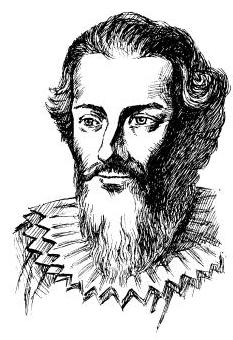
\includegraphics[max width=0.2\textwidth]{images/bo_d7fr3gc91nqc7381iccg_35_1183_1005_233_340_0.jpg}
\end{center}
\hspace*{3em} 

韦达 (F. Viete, 1540- 1603), 法国数学家.

\HRule

例 4 告诉我们, 给定了一个一元二次方程的系数, 就可以确定该方程的根和解集. 反过来, 如果已知一个一元二次方程的两个根, 能否确定此方程的系数呢? 描述一元二次方程根与系数关系的韦达定理就回答了这一问题.

韦达定理 若一元二次方程 \(a{x}^{2} + {bx} + c = 0\left( {a \neq  0}\right)\) 的两个根为 \({x}_{1}\text{ 、 }{x}_{2}\) ,则

\[
{x}_{1} + {x}_{2} =  - \frac{b}{a},{x}_{1}{x}_{2} = \frac{c}{a}.
\]

证明 因为一元二次方程 \(a{x}^{2} + {bx} + c = 0\) 的两个根为 \({x}_{1}\) 、 \({x}_{2}\) ,所以二次三项式 \(a{x}^{2} + {bx} + c\) 可以因式分解为

\[
a{x}^{2} + {bx} + c = a\left( {x - {x}_{1}}\right) \left( {x - {x}_{2}}\right) .
\]

\HRule

请用求根公式验证韦达定理.

\HRule

由于

\[
a\left( {x - {x}_{1}}\right) \left( {x - {x}_{2}}\right)  = a{x}^{2} - a\left( {{x}_{1} + {x}_{2}}\right) x + a{x}_{1}{x}_{2},
\]

从而等式 \(a{x}^{2} + {bx} + c = a{x}^{2} - a\left( {{x}_{1} + {x}_{2}}\right) x + a{x}_{1}{x}_{2}\) 恒成立. 由例 5 知, 该等式两边的对应项系数应相等. 因此

\[
{x}_{1} + {x}_{2} =  - \frac{b}{a},{x}_{1}{x}_{2} = \frac{c}{a}.
\]

例 6 已知方程 \({x}^{2} + x - 3 = 0\) 的两个根为 \({x}_{1}\text{ 、 }{x}_{2}\) ,求下列各式的值:



\section*{}

(1) \({x}_{1}^{2}{x}_{2} + {x}_{2}^{2}{x}_{1}\) ； (2) \(\left| {{x}_{1} - {x}_{2}}\right|\) .

解 由韦达定理,得 \({x}_{1} + {x}_{2} =  - 1,{x}_{1}{x}_{2} =  - 3\) .

(1) \({x}_{1}^{2}{x}_{2} + {x}_{2}^{2}{x}_{1} = {x}_{1}{x}_{2}\left( {{x}_{1} + {x}_{2}}\right)  =  - 3 \times  \left( {-1}\right)  = 3\) .

(2) \(\left| {{x}_{1} - {x}_{2}}\right|  = \sqrt{{\left( {x}_{1} - {x}_{2}\right) }^{2}} = \sqrt{{\left( {x}_{1} + {x}_{2}\right) }^{2} - 4{x}_{1}{x}_{2}}\)

\(= \sqrt{{\left( -1\right) }^{2} - 4 \times  \left( {-3}\right) } = \sqrt{13}.\)

\section*{练习 2.1(2)}

1. 求一元二次方程 \(a{x}^{2} - {4x} + 2 = 0\left( {a \neq  0}\right)\) 的解集.

2. 已知方程 \(2{x}^{2} + {4x} - 3 = 0\) 的两个根为 \({x}_{1}\text{ 、 }{x}_{2}\) ,求下列各式的值:

(1) \({x}_{1}^{2}{x}_{2} + {x}_{2}^{2}{x}_{1}\) ；

(2) \(\frac{1}{{x}_{1}} + \frac{1}{{x}_{2}}\) ；

(3) \({x}_{1}^{2} + {x}_{2}^{2}\) ； (4) \({x}_{1}^{3} + {x}_{2}^{3}\) .

\section*{3 不等式的性质}

两个实数之间不仅可以有相等关系, 还可以有大小关系.

对于两个实数 \(a\text{ 、 }b\) ,如果 \(b - a\) 是正数,就称 \(b\) 大于 \(a\) ,记为 \(b > a\) ; 如果 \(b - a\) 是负数,就称 \(b\) 小于 \(a\) ,记为 \(b < a\) ; 如果 \(b - a\) 是零,就称 \(b\) 等于 \(a\) ,记为 \(b = a\) . 这就是说

\[
b > a \Leftrightarrow  b - a > 0;
\]

\[
b = a \Leftrightarrow  b - a = 0;
\]

\[
b < a \Leftrightarrow  b - a < 0.
\]

这是研究一切不等式的基础.

显然,对于任意给定的两个实数 \(a\text{ 、 }b\) ,

\[
b > a \Leftrightarrow  a < b\text{ . }
\]

根据实数的大小关系,对任何两个给定的实数 \(a\text{ 、 }b\) ,或者 \(a > b\) ,或者 \(a < b\) ,或者 \(a = b\) ,三者中有且只有一种情况成立.

通常,符号 \(b \geq  a\) (读作 \(b\) 大于等于 \(a\) )表示 \(b > a\) 或 \(b = a\) ; 符号 \(b \leq  a\) (读作 \(b\) 小于等于 \(a\) )表示 \(b < a\) 或 \(b = a\) .

大于号>,小于号<,大于等于号>,小于等于号 \(\leq\) 都称为不等号. 用不等号将两个表达式连接起来, 就得到一个不等式 (inequality).

根据实数间的大小关系, 类比于等式性质, 我们可以得到不

\section*{}

等式的基本性质.

(1)传递性 设 \(a\text{ 、 }b\text{ 、 }c\) 均为实数，

如果 \(a > b\) ,且 \(b > c\) ,那么 \(a > c\) .

证明 因为 \(a > b\) ,所以 \(a - b > 0\) .

同理,由 \(b > c\) ,有 \(b - c > 0\) .

由于两个正数的和是正数, 于是

\[
a - c = \left( {a - b}\right)  + \left( {b - c}\right)  > 0,
\]

即 \(a > c\) .

(2)加法性质 设 \(a\text{ 、 }b\text{ 、 }c\) 均为实数，

Q

如果 \(a > b\) ,那么 \(a + c > b + c\) .

证明 因为 \(a > b\) ,所以 \(a - b > 0\) .

于是有 \(\;\left( {a + c}\right)  - \left( {b + c}\right)  = a - b > 0\) , Q

即 \(a + c > b + c\) .

(3)乘法性质 设 \(a\text{ 、 }b\text{ 、 }c\) 均为实数，

如果 \(a > b\) ,且 \(c > 0\) ,那么 \({ac} > {bc}\) ;

如果 \(a > b\) ,且 \(c < 0\) ,那么 \({ac} < {bc}\) .

?

证明 显然, \({ac} - {bc} = \left( {a - b}\right) c\) .

因为 \(a > b\) ,所以 \(a - b > 0\) .

当 \(c > 0\) 时， \(\left( {a - b}\right) c > 0\) ，所以 \({ac} > {bc}\) ；

当 \(c < 0\) 时， \(\left( {a - b}\right) c < 0\) ，所以 \({ac} < {bc}\) .

例 7 证明: 如果 \(a + b > c\) ,那么 \(a > c - b\) ; 反之亦然.

证明 若 \(a + b > c\) ,利用不等式的加法性质,在不等式两边同加 \(- b\) ,即得 \(a > c - b\) .

反过来,若 \(a > c - b\) ,仍利用不等式的加法性质,在不等式两边同加 \(b\) ,即得 \(a + b > c\) .

例 7 表明, 将不等式中的任一项改变符号后, 可以从不等式的一边移到不等式的另一边. 在研究不等式时, 移项常用于化简一个不等式.



\HRule

不等式加法性质表明:在不等式的两边加上 (或减去) 同一个实数, 不等号的方向不变.

不等式乘法性质表明:在不等式的两边乘 (或除以) 同一个正数，不等号的方向不变. 但若乘 (或除以) 同一个负数, 不等号的方向要改变.

等式与不等式的性质有什么相同点和不同点?

\HRule



Q 例 8 已知 \(a > b,c > d\) . 求证: \(a + c > b + d\) .

证明 因为 \(a > b,c > d\) ,所以 \(a - b > 0,c - d > 0\) .

\HRule

例 8 表明, 由

\(a > b,c > d\)

可推出

\(a + c > b + d\) .

这称为不等式的同向可加性.

\HRule

于是

\[
\left( {a + c}\right)  - \left( {b + d}\right)  = \left( {a - b}\right)  + \left( {c - d}\right)  > 0,
\]

即 \(a + c > b + d\) .

例 9 已知 \(a > b,c > d\) . 求证: \(a - d > b - c\) .

证明 因为 \(a > b,c > d\) ,所以 \(a - b > 0,c - d > 0\) .

于是

\[
a - d - \left( {b - c}\right)  = \left( {a - b}\right)  + \left( {c - d}\right)  > 0,
\]

即 \(a - d > b - c\) .

?

例10 (1)已知 \(a > b > 0\) ，求证: \(\frac{1}{b} > \frac{1}{a} > 0\) ；

\HRule

较大的数的倒数是否一定比较小的数的倒数小?

\HRule

(2)已知 \(a > b > 0,c > d > 0\) . 求证: \(\frac{a}{d} > \frac{b}{c}\) .

证明 (1) 因为 \(a > b > 0\) ,所以 \({ab} > 0\) .

由不等式的乘法性质,在不等式 \(a > b\) 的两边同时乘 \(\frac{1}{ab}\) ,得 \(\frac{a}{ab} > \frac{b}{ab}\) ,即 \(\frac{1}{b} > \frac{1}{a} > 0\) .

(2)因为 \(c > d > 0\) ，利用(1)的结论，有 \(\frac{1}{d} > \frac{1}{c} > 0\) .

又因为 \(a > b > 0\) ,由不等式的乘法性质,有 \(\frac{a}{d} > \frac{a}{c} > 0\) 及 \(\frac{a}{c} > \frac{b}{c} > 0\) ,从而由不等式的传递性得到 \(\frac{a}{d} > \frac{b}{c}\) .

\section*{练习 2.1(3)}

1. 设 \(a\text{ 、 }b\text{ 、 }c\text{ 、 }d\) 为实数,判断下列命题的真假,并说明理由:

(1)如果 \(a > b,c > d\) ,那么 \(a + d > b + c\) ;

(2)如果 \({ab} > {ac}\) ，那么 \(b > c\) ；

(3)如果 \(a \geq  b\) 且 \(a \leq  b\) ，那么 \(a = b\) ；

(4)如果 \(a > b,\frac{1}{c} > \frac{1}{d}\) ，那么 \(\frac{a}{c} > \frac{b}{d}\) ；

(5)如果 \(\frac{b}{a} > \frac{d}{c}\) ，那么 \({bc} > {ad}\) .

2. 设 \({ab} > 0\) ,求证: \(a > b\) 是 \(\frac{1}{a} < \frac{1}{b}\) 的充要条件.



例 11 (1)已知 \(a > b > 0,c > d > 0\) . 求证: \({ac} > {bd}\) ；

(2)已知 \(a > b > 0\) ，求证: \({a}^{n} > {b}^{n}\) ，其中 \(n\) 是正整数.

证明 (1) 因为 \(a > b,c > 0\) ,所以 \({ac} > {bc}\) . 又因为 \(c > d\) , \(b > 0\) ,所以 \({bc} > {bd}\) . 由不等式的传递性,得 \({ac} > {bd}\) .

(2)将(1)结论中的 \(c\) 换成 \(a\) ， \(d\) 换成 \(b\) ，就得到 \({a}^{2} > {b}^{2} > 0\) . 结合 \(a > b > 0\) ,再次利用(1)的结论，可得 \({a}^{3} > {b}^{3} > 0\) ,反复运用 (1)的结论，最终就得到 \({a}^{n} > {b}^{n}\) .

例 12 已知 \(a\text{ 、 }b\) 为正数， \(n\) 为正整数. 求证:如果 \({a}^{n} > {b}^{n}\) ,那么 \(a > b\) .

证明 利用反证法. 首先根据实数的性质可知,在 \(a > b\) , \(a < b\) 及 \(a = b\) 三者中有且仅有一个成立. 假定结论 \(a > b\) 不成立, 那么或者 \(a < b\) ,或者 \(a = b\) .

如果 \(a < b\) ,由于 \(a\text{ 、 }b\) 都是正数,利用例 11 (2) 的结论,那么两边 \(n\) 次乘方，可得 \({a}^{n} < {b}^{n}\) ，与假设 \({a}^{n} > {b}^{n}\) 矛盾；

如果 \(a = b\) ,两边 \(n\) 次乘方得 \({a}^{n} = {b}^{n}\) ,同样与假设 \({a}^{n} > {b}^{n}\) 矛盾.

综上所述， \(a \leq  b\) 不可能成立，因此 \(a > b\) .

为比较两个实数的大小，常用的方法是判定这两个数的差的符号. 要比较两个表达式 \(A\) 及 \(B\) 的大小，同样可以采用类似的方法. 例如,要证明 \(A > B\) ,只需证明 \(A - B > 0\) ; 同样地,要证明 \(A < B\) ,只需证明 \(A - B < 0\) .

定理 对任意的实数 \(a\) 和 \(b\) ，总有

\[
{a}^{2} + {b}^{2} \geq  {2ab},
\]

且等号当且仅当 \(a = b\) 时成立.

证明 因为

\[
{a}^{2} + {b}^{2} - {2ab} = {\left( a - b\right) }^{2} \geq  0,
\]

所以

\[
{a}^{2} + {b}^{2} \geq  {2ab},
\]

而且当且仅当 \(a - b = 0\) 即 \(a = b\) 时,不等式中等号成立.

例 13 设 \(a\) 是实数,比较 \({\left( a + 1\right) }^{2}\) 与 \({a}^{2} - a + 1\) 的值的大小.

解 \({\left( a + 1\right) }^{2} - \left( {{a}^{2} - a + 1}\right)  = {a}^{2} + {2a} + 1 - {a}^{2} + a - 1 = {3a}\) .



\section*{}

当 \(a > 0\) 时， \({\left( a + 1\right) }^{2} > {a}^{2} - a + 1\) ；

当 \(a = 0\) 时， \({\left( a + 1\right) }^{2} = {a}^{2} - a + 1\) ；

当 \(a < 0\) 时， \({\left( a + 1\right) }^{2} < {a}^{2} - a + 1\) .

\section*{练习 2.1(4)}

1. 设 \(a\text{ 、 }b\text{ 、 }c\) 是实数,判断下列命题的真假,并说明理由.

(1)如果 \(a{c}^{2} > b{c}^{2}\) ，那么 \(a > b\) ；

(2)如果 \({ab} > c\) ，那么 \(a > \frac{c}{b}\) ；

(3)如果 \(a > b \geq  0\) ，那么 \(\sqrt{a} > \sqrt{b}\) .

2. 设 \(x\) 是实数,比较 \({x}^{2} + 4\) 与 \({4x}\) 的值的大小.

\section*{习题 2.1}

\section*{A 组}

1. 设 \(a \in  \mathbf{R}\) ,求关于 \(x\) 的方程 \({ax} = 2\) 的解集.

2. 设 \(k \in  \mathbf{R}\) ,求关于 \(x\) 与 \(y\) 的二元一次方程组 \(\left\{  \begin{array}{l} y =  - {2x} + 1, \\  y = {kx} - 3 \end{array}\right.\) 的解集.

3. 设 \(a \in  \mathbf{R}\) ,求一元二次方程 \({x}^{2} - {2ax} + {a}^{2} - 4 = 0\) 的解集.

4. 已知等式 \(2{x}^{2} + {3x} + 5 = a\left( {{2x} + 1}\right) \left( {x + 1}\right)  + c\) 恒成立,求常数 \(a\text{ 、 }c\) 的值.

5. 已知一元二次方程 \(a{x}^{2} + {bx} + c = 0\left( {a \neq  0}\right)\) 的两实根为 \({x}_{1}\text{ 、 }{x}_{2}\) ,求证:

\[
\left| {{x}_{2} - {x}_{1}}\right|  = \frac{\sqrt{{b}^{2} - {4ac}}}{\left| a\right| }.
\]

6. 已知一元二次方程 \({x}^{2} + {3x} - 3 = 0\) 的两个实根分别为 \({x}_{1}\text{ 、 }{x}_{2}\) ，求作二次项系数是 1 , 且分别以下列数值为根的一元二次方程:

(1) \(- {x}_{1}, - {x}_{2}\) ； (2) \(2{x}_{1} + 1,2{x}_{2} + 1\) ；

(3) \(\frac{1}{{x}_{1}},\frac{1}{{x}_{2}}\) ； (4) \({x}_{1}^{2},{x}_{2}^{2}\) .

7. 设 \(a\text{ 、 }b\text{ 、 }c\text{ 、 }d\) 为实数，判断下列命题的真假:

(1)若 \(a > b \geq  0\) ，则 \({a}^{2} > {b}^{2}\) ；

(2)若 \(\sqrt{a} > \sqrt{b}\) ，则 \(a > b\) ；

(3)若 \(a > b > 0,c > d > 0\) ，则 \(\frac{a}{c} > \frac{b}{d}\) ；

(4)若 \(\frac{b}{a} > 0\) ，则 \({ab} > 0\) ；

(5)若 \(a > b > 0\) ，则 \({a}^{2} > {ab} > {b}^{2}\) ；

(6)若 \(\sqrt{a} > b\) ，则 \(a > {b}^{2}\) .

8. 选择题:

(1)如果 \({a}^{2} > {b}^{2}\) ，那么下列不等式中成立的是 ( )

A. \(a > 0 > b\) ； B. \(a > b > 0\) ； C. \(\left| a\right|  > \left| b\right|\) ; D. \(a > \left| b\right|\) .

(2)如果 \(a < b < 0\) ，那么下列不等式中成立的是 ( )

A. \(\frac{a}{b} < 1\) ; B. \({a}^{2} > {ab}\) ;

C. \(\frac{1}{{b}^{2}} < \frac{1}{{a}^{2}}\) ; D. \(\frac{1}{a} < \frac{1}{b}\) .

(3)如果 \(a < 0 < b\) ，那么下列不等式中成立的是 ( )

A. \(\sqrt{-a} < \sqrt{b}\) ; B. \({a}^{2} < {b}^{2}\) ; C. \({a}^{3} < {b}^{3}\) ; D. \({ab} > {b}^{2}\) .

9. 证明: “ \(a > 0\) 且 \(b > 0\) ” 是 “ \(a + b > 0\) 且 \({ab} > 0\) ” 的充要条件.

10. 设 \(x\) 是实数，比较 \(\left( {x + 1}\right) \left( {{x}^{2} - x + 1}\right)\) 与 \(\left( {x - 1}\right) \left( {{x}^{2} + x + 1}\right)\) 的值的大小.

11. 试比较下列各数的大小, 并说明理由:

(1)3+√3 与 2+√5 ; (2) \(\sqrt{3} + \sqrt{5}\) 与 \(\sqrt{2} + \sqrt{6}\) .

12. 设 \(a\text{ 、 }b\) 为实数,比较 \({a}^{2} + {b}^{2}\) 与 \({2a} - {2b} - 2\) 的值的大小.

13. 已知 \(a > b,c > d\) . 求证: \({ac} + {bd} > {ad} + {bc}\) .

14. 已知 \(a \geq   - 1\) ,求证: \({a}^{3} + 1 \geq  {a}^{2} + a\) .

15. 已知 \(a\text{ 、 }b\) 为任意给定的正数,求证: \({a}^{3} + {b}^{3} \geq  a{b}^{2} + b{a}^{2}\) ,并指出等号成立的条件.

\section*{B 组}

1. 设 \(a\) 为实数,求关于 \(x\) 的方程 \({2x} + {a}^{2} = {ax} + 4\) 的解集.

2. 设 \(m\) 为实数，求关于 \(x\) 的方程 \(\left( {m + 1}\right) {x}^{2} + {6mx} + {9m} = 1\) 的解集.

3. 已知等式 \(2{x}^{2} - {3x} - 1 = a{\left( x - 1\right) }^{2} + b\left( {x - 1}\right)  + c\) 恒成立,其中 \(a\text{ 、 }b\text{ 、 }c\) 为常数. 求 \(a - b + c\) 的值.

4. 对一元二次方程 \(a{x}^{2} + {bx} + c = 0\left( {a \neq  0}\right)\) ,证明: \({ac} < 0\) 是该方程有两个异号实根的充要条件.

5. 已知一元二次方程 \(2{x}^{2} + x - 3 = 0\) 的两个实根分别为 \({x}_{1}\text{ 、 }{x}_{2}\) ,求作二次项系数是 1 , 且分别以下列数值为根的一元二次方程:

(1) \({x}_{1} + {x}_{2},{x}_{1}{x}_{2}\) ； (2) \(2{x}_{1}^{2} + 1,2{x}_{2}^{2} + 1\) ；

(3) \(\frac{{x}_{2}}{{x}_{1}},\frac{{x}_{1}}{{x}_{2}}\) ； (4) \({x}_{1}^{4},{x}_{2}^{4}\) .

\section*{}

6. 已知一元二次方程 \({x}^{2} - {2mx} + m - 1 = 0\) 的两实根为 \({x}_{1}\text{ 、 }{x}_{2}\) ，且 \({x}_{1}^{2} + {x}_{2}^{2} = 4\) . 求实数 \(m\) 的值.

7. 已知实数 \(a\text{ 、 }b\text{ 、 }c\) 满足 \(a + b + c = 0\) ,且 \(a > b > c\) . 求证: \(a > 0\) 且 \(c < 0\) .

8. 设 \(s = a + b,p = {ab}\left( {a\text{ 、 }b \in  \mathbf{R}}\right)\) ,写出 “ \(a > 1\) 且 \(b > 1\) ” 用 \(s\text{ 、 }p\) 表示的一个充要条件, 并证明.

9. 原有酒精溶液 \(a\) (单位: \(\mathrm{g}\) ),其中含有酒精 \(b\) (单位: \(\mathrm{g}\) ),其酒精浓度为 \(\frac{b}{a}\) . 为增加酒精浓度,在原溶液中加入酒精 \(x\) (单位: \(\mathrm{g}\) ),新溶液的浓度变为 \(\frac{b + x}{a + x}\) . 根据这一事实, 可提炼出如下关于不等式的命题: 若 \(a > b > 0,x > 0\) ,则 \(\frac{b}{a} < \frac{b + x}{a + x} < 1\) . 试加以证明.



\section*{2.2 不等式的求解}

在含有未知数的不等式中, 能使此不等式成立的未知数的值称为该不等式的解 (solution of an inequality). 一个不等式的解的全体所组成的集合称为此不等式的解集 (solution set of an inequality). 求不等式解集的过程称为不等式的求解或解不等式 (solve an inequality). 将含有相同未知数的多个不等式联立起来, 就得到不等式组. 解不等式组就是求不等式组中的所有不等式的解集的交集.

解方程时, 往往要先将原先比较复杂的方程变形化为较简单的方程, 再通过解这个比较简单的方程来求出原方程的解. 同理, 解不等式时, 常常要通过等价变形, 将原不等式化为较简单的不等式或不等式组, 从而求得原不等式的解集.

1

\section*{一元一次不等式及 一元一次不等式组的求解}

例 1 设 \(a\) 为实数，求关于 \(x\) 的不等式 \({ax} < 1\) 的解集.

解 由不等式的性质,可得:

当 \(a > 0\) 时,解集为 \(\left( {-\infty ,\frac{1}{a}}\right)\) ;

当 \(a = 0\) 时,解集为 \(\mathbf{R}\) ;

当 \(a < 0\) 时,解集为 \(\left( {\frac{1}{a}, + \infty }\right)\) .

例 2 设 \(a\) 为实数，解关于 \(x\) 的一元一次不等式组

\[
\left\{  \begin{array}{l} {2x} + a > 0, \\  {3x} - {6a} < 0. \end{array}\right.
\]

解 根据不等式的性质,原不等式组等价于 \(\left\{  \begin{array}{l} {2x} >  - a, \\  {3x} < {6a}, \end{array}\right.\) 整理得





Q

\[
\left\{  \begin{array}{l} x >  - \frac{a}{2}, \\  x < {2a}. \end{array}\right.
\]

因此,当 \(a > 0\) 时,解集为 \(\left( {-\frac{a}{2},{2a}}\right)\) ; 当 \(a \leq  0\) 时,解集为 \(\varnothing\) .

\section*{2 一元二次不等式的求解}

在交通事故中, 交通管理部门往往通过测量肇事汽车的刹车距离来推断该车辆实施刹车前的行驶速度, 并作为断定司机在肇事前是否有超速违章行为的重要参考依据.

Q

假设在某次交通事故中, 测得肇事汽车的刹车距离大于 \({20}\mathrm{\;m}\) ,试推断该汽车在刹车前的车速是否超过该水泥道路上机动车的限速规定 \({30}\mathrm{{km}}/\mathrm{h}\) . 在一般情况下,我们可以采用如下数学模型来描述该种型号的汽车在常规水泥路面上的刹车距离 \(d\) (单位: \(\mathrm{m}\) ) 与刹车前的车速 \(v\) (单位: \(\mathrm{{km}}/\mathrm{h}\) ) 之间的关系:

\[
d = {0.2085v} + {0.0064}{v}^{2}.
\]

因此,我们需要通过求解不等式 \({0.2085v} + {0.0064}{v}^{2} > {20}\) 来判断 \(v\) 是否大于 \({30}\mathrm{\;{km}}/\mathrm{h}\) . 这就是一个一元二次不等式的求解问题.

定义 设 \(a\text{ 、 }b\text{ 、 }c\) 为实数,且 \(a \neq  0\) ,形如

\[
a{x}^{2} + {bx} + c > 0\left( { < 0, \geq  0\text{ 或 } \leq  0}\right)
\]

的不等式统称为一元二次不等式 (quadratic inequality in one variable).

让我们先来看两个例子.

例 3 解不等式 \(\left( {x - 3}\right) \left( {x + 1}\right)  > 0\) .

解 利用不等式的性质,原不等式等价于两个一次式 \(x - 3\) 和 \(x + 1\) 同号,即等价于不等式组 \(\left\{  \begin{array}{l} x + 1 > 0, \\  x - 3 > 0 \end{array}\right.\) 或 \(\left\{  \begin{array}{l} x + 1 < 0, \\  x - 3 < 0. \end{array}\right.\)

由此得 \(\left\{  \begin{array}{l} x >  - 1, \\  x > 3 \end{array}\right.\) 或 \(\left\{  \begin{array}{l} x <  - 1, \\  x < 3. \end{array}\right.\)



\HRule

我们可以在数轴上表示例 2 中的不等式组的解集, 如图 2-2-1 所示.

\begin{center}
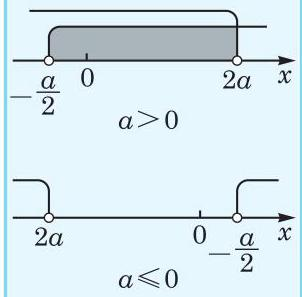
\includegraphics[max width=0.2\textwidth]{images/bo_d7fr3gc91nqc7381iccg_44_196_436_302_297_0.jpg}
\end{center}
\hspace*{3em} 

图 2-2-1

此刹车案例参考了由吉奥丹诺(F. R. Giordano)等著、叶其孝等译的《数学建模》 一书，为便于理解， 原始模型中的距离单位英里、英尺换算为千米、米，参数值也做了相应调整.

请参照图 2-2-1, 在数轴上表示出例 3 的解集.

\HRule

因此, 原不等式的解集为这两个不等式组解集的并集 \(\left( {-\infty , - 1}\right)  \cup  \left( {3, + \infty }\right)\) .

例 4 解不等式 \(\left( {x - 1}\right) \left( {x + 4}\right)  < 0\) .

解 利用不等式的性质, 原不等式等价于

\[
\left\{  {\begin{array}{l} x - 1 < 0, \\  x + 4 > 0 \end{array}\text{ 或 }\left\{  \begin{array}{l} x - 1 > 0, \\  x + 4 < 0. \end{array}\right. }\right.
\]

由第一组不等式,得 \(\left\{  \begin{array}{l} x < 1, \\  x >  - 4, \end{array}\right.\) 其解集为 \(\left( {-4,1}\right)\) ; 而由第二组不等式,得 \(\left\{  \begin{array}{l} x > 1, \\  x <  - 4, \end{array}\right.\) 其解集为 \(\varnothing\) .

因此,原不等式的解集为 \(\left( {-4,1}\right)\) .

下面，我们来讨论如何求解一般的一元二次不等式

\[
a{x}^{2} + {bx} + c > 0\text{ 与 }a{x}^{2} + {bx} + c < 0.
\]

不失一般性，我们总假设二次项系数 \(a > 0\) . 因为当 \(a < 0\) 时，只要在原不等式两边同乘 -1 ，并改变不等号的方向，就可以转化为 \(a > 0\) 的情形.

通过例 3 和例 4，我们可以发现:一元二次不等式的求解与相应的一元二次方程的求解密切相关.

事实上,当 \(\Delta  = {b}^{2} - {4ac} > 0\) 时,一元二次方程 \(a{x}^{2} + {bx} + \; c = 0\) 有两个不同的实根,记为 \({x}_{1}\text{ 、 }{x}_{2}\) ,其中 \({x}_{1} < {x}_{2}\) . 利用因式分解,不等式 \(a{x}^{2} + {bx} + c > 0\) 等价于 \(a\left( {x - {x}_{1}}\right) \left( {x - {x}_{2}}\right)  > 0\) ,且由于 \(a > 0\) ,原不等式等价于 \(\left( {x - {x}_{1}}\right) \left( {x - {x}_{2}}\right)  > 0\) . 类似于例 3, 易知不等式 \(a{x}^{2} + {bx} + c > 0\) 的解集为 \(\left( {-\infty ,{x}_{1}}\right)  \cup  \left( {{x}_{2}, + \infty }\right)\) . 相应地,不等式 \(a{x}^{2} + {bx} + c < 0\) 等价于 \(\left( {x - {x}_{1}}\right) \left( {x - {x}_{2}}\right)  < 0\) . 类似于例 4,易知不等式 \(a{x}^{2} + {bx} + c < 0\) 的解集为 \(\left( {{x}_{1},{x}_{2}}\right)\) .

同理,当 \(a > 0\) 时,不等式 \(a{x}^{2} + {bx} + c \geq  0\) 等价于 \(\left( {x - {x}_{1}}\right) \; \left( {x - {x}_{2}}\right)  \geq  0\) ,其解集为 \(\left( {-\infty ,{x}_{1}\rbrack \cup \lbrack {x}_{2}, + \infty }\right)\) ; 而不等式 \(a{x}^{2} + {bx} + c \leq  0\) 等价于 \(\left( {x - {x}_{1}}\right) \left( {x - {x}_{2}}\right)  \leq  0\) ,其解集为 \(\left\lbrack  {{x}_{1},{x}_{2}}\right\rbrack\) .

设方程 \(a{x}^{2} + {bx} + c = 0\left( {a > 0}\right)\) 的判别式 \(\Delta  = {b}^{2} - {4ac} > 0\) , 其两根记为 \({x}_{1}\text{ 、 }{x}_{2}\) ,且 \({x}_{1} < {x}_{2}\) ,则可将上述不等式的求解结果总结成表 2-1:





表 2-1

\begin{center}
\adjustbox{max width=\textwidth}{
\begin{tabular}{|c|c|}
\hline
\multicolumn{2}{|c|}{\(a > 0,\Delta  > 0\)} \\
\cline{1-2}
\(a{x}^{2} + {bx} + c > 0\) & 解集为 \(\left( {-\infty ,{x}_{1}}\right)  \cup  \left( {{x}_{2}, + \infty }\right)\) \\
\cline{1-2}
\(a{x}^{2} + {bx} + c < 0\) & 解集为 \(\left( {{x}_{1},{x}_{2}}\right)\) \\
\cline{1-2}
\(a{x}^{2} + {bx} + c \geq  0\) & 解集为 \(\left( {-\infty ,{x}_{1}}\right\rbrack   \cup  \left\lbrack  {{x}_{2}, + \infty }\right)\) \\
\cline{1-2}
\(a{x}^{2} + {bx} + c \leq  0\) & 解集为 \(\left\lbrack  {{x}_{1},{x}_{2}}\right\rbrack\) \\
\cline{1-2}
\hline
\end{tabular}
}
\end{center}

例 5 解不等式 \(- 2{x}^{2} + {3x} - \frac{1}{2} \geq  0\) .

解 将不等式两边乘 -1,原不等式就化为 \(2{x}^{2} - {3x} + \frac{1}{2} \leq  0\) . 相应的一元二次方程 \(2{x}^{2} - {3x} + \frac{1}{2} = 0\) 的两根为 \(\frac{3 \pm  \sqrt{5}}{4}\) .

对照表 2-1,可知原不等式的解集为 \(\left\lbrack  {\frac{3 - \sqrt{5}}{4},\frac{3 + \sqrt{5}}{4}}\right\rbrack\) .

对前面提到的判别超速问题, 只要求出相应的一元二次不等式 \({0.2085v} + {0.0064}{v}^{2} > {20}\) 的解集即可. 利用前面的方法,容易解得 \(v < \frac{-{0.2085} - \sqrt{{0.2085}^{2} - 4 \times  {0.0064} \times  \left( {-{20}}\right) }}{2 \times  {0.0064}}\mathrm{\;{km}}/\mathrm{h}\) (舍去) 或 \(v > \frac{-{0.2085} + \sqrt{{0.2085}^{2} - 4 \times  {0.0064} \times  \left( {-{20}}\right) }}{2 \times  {0.0064}}\mathrm{\;{km}}/\mathrm{h}\) (约为 41.9 km/h).

由此可推断出该肇事汽车在刹车前的车速大于 \({41}\mathrm{\;{km}}/\mathrm{h}\) ,超过该道路上机动车的限速规定 \({30}\mathrm{\;{km}}/\mathrm{h}\) . 这个推断将成为交通管理部门认定事故责任的重要依据之一.

\section*{练习 2.2(1)}

1. 设 \(a \neq  1\) ,解关于 \(x\) 的不等式: \({ax} < {a}^{2} + x - 1\) .

2. 填空题:

(1) \(\left( {x - 2}\right) \left( {x + 3}\right)  < 0\) 的解集是\_\_\_\_\_；

(2) \(\left( {2 - x}\right) \left( {x + 3}\right)  < 0\) 的解集是\_\_\_\_\_.

(3) \(\left( {x - 2}\right) \left( {x + 3}\right)  \geq  0\) 的解集是\_\_\_\_\_.

3. 求下列不等式的解集:

(1)一 \({8x} \leq  3{x}^{2} + 4\) ； (2) \(- {x}^{2} < {2x} - 4\) .



一元二次不等式的求解与相应的一元二次方程的求解紧密相关. 我们已经知道,当 \(\Delta  = {b}^{2} - {4ac} > 0\) 时,如何求解不等式 \(a{x}^{2} + {bx} + c > 0\left( { < 0, \geq  0\text{ 或 } \leq  0}\right)\) . 那么,当 \(\Delta  = {b}^{2} - {4ac} \leq  0\) 时, 情况又如何呢?

不失一般性,我们仍然只讨论 \(a > 0\) 的情形.

先看两个简单的例子: \({x}^{2} > 0\) 的解集为 \(\left( {-\infty ,0}\right)  \cup \; \left( {0, + \infty }\right)\) ,而 \({\left( x - 1\right) }^{2} + 1 < 0\) 的解集为 \(\varnothing\) .

再看一般的情况，首先讨论 \(\Delta  = {b}^{2} - {4ac} = 0\) 的情形. 这时，一元二次方程 \(a{x}^{2} + {bx} + c = 0\) 有重根 \({x}_{1} = {x}_{2} =  - \frac{b}{2a}\) . 由因式分解, 不等式 \(a{x}^{2} + {bx} + c > 0\) 等价于 \(a{\left( x - {x}_{1}\right) }^{2} > 0\) . 又由于 \(a > 0\) ,原不等式等价于 \({\left( x - {x}_{1}\right) }^{2} > 0\) ,其解集为 \(\left( {-\infty ,{x}_{1}}\right)  \cup  \left( {{x}_{1}, + \infty }\right)\) . 相应地,不等式 \(a{x}^{2} + {bx} + c < 0\) 等价于 \({\left( x - {x}_{1}\right) }^{2} < 0\) ,其解集为 \(\varnothing\) .

同理,不等式 \(a{x}^{2} + {bx} + c \geq  0\) 等价于 \({\left( x - {x}_{1}\right) }^{2} \geq  0\) ,其解集为 \(\mathbf{R}\) ; 而不等式 \(a{x}^{2} + {bx} + c \leq  0\) 等价于 \({\left( x - {x}_{1}\right) }^{2} \leq  0\) ,其解集为 \(\left\{  {x}_{1}\right\}\) .

其次讨论 \(\Delta  = {b}^{2} - {4ac} < 0\) 的情形. 这时,一元二次方程 \(a{x}^{2} + {bx} + c = 0\) 没有实根. \(a{x}^{2} + {bx} + c\) 无法在实数范围内因式分解. 由配方法,不等式 \(a{x}^{2} + {bx} + c > 0\) 等价于 \(a{\left( x + \frac{b}{2a}\right) }^{2} + \; \frac{{4ac} - {b}^{2}}{4a} > 0\) ,移项并在不等式两边同时除以 \(a\) ,可得 \({\left( x + \frac{b}{2a}\right) }^{2} > \; \frac{{b}^{2} - {4ac}}{4{a}^{2}}\) . 因为 \(\Delta  < 0,\frac{{b}^{2} - {4ac}}{4{a}^{2}} < 0\) ,所以上述不等式的解集为 \(\mathbf{R}\) . 相应地,不等式 \(a{x}^{2} + {bx} + c < 0\) 等价于 \({\left( x + \frac{b}{2a}\right) }^{2} < \frac{{b}^{2} - {4ac}}{4{a}^{2}}\) ,其解集为 \(\varnothing\) .

同理,不等式 \(a{x}^{2} + {bx} + c \geq  0\) 等价于 \({\left( x + \frac{b}{2a}\right) }^{2} \geq  \frac{{b}^{2} - {4ac}}{4{a}^{2}}\) ,其解集为 \(\mathbf{R}\) ; 而不等式 \(a{x}^{2} + {bx} + c \leq  0\) 等价于 \({\left( x + \frac{b}{2a}\right) }^{2} \leq  \frac{{b}^{2} - {4ac}}{4{a}^{2}}\) , 其解集为 \(\varnothing\) .

上述结果可总结成表 2-2:



表 2-2

\begin{center}
\adjustbox{max width=\textwidth}{
\begin{tabular}{|c|c|c|c|}
\hline
\multicolumn{2}{|c|}{\(a > 0,\Delta  = 0\)} & \multicolumn{2}{|c|}{\(a > 0,\Delta  < 0\)} \\
\cline{1-4}
\(a{x}^{2} + {bx} + c > 0\) & 解集为 \(\left( {-\infty ,{x}_{1}}\right) \; \bigcup \left( {{x}_{1}, + \infty }\right)\) & \(a{x}^{2} + {bx} + c > 0\) & 解集为 \(R\) \\
\cline{1-4}
\(a{x}^{2} + {bx} + c < 0\) & 解集为 \(\varnothing\) & \(a{x}^{2} + {bx} + c < 0\) & 解集为 \(\mathbf{R}\) \\
\cline{1-4}
\(a{x}^{2} + {bx} + c \geq  0\) & 解集为 \(\mathbf{R}\) & \(a{x}^{2} + {bx} + c \geq  0\) & 解集为 \(\mathbf{R}\) \\
\cline{1-4}
\(a{x}^{2} + {bx} + c \leq  0\) & 解集为 \(\left\{  {x}_{1}\right\}\) & \(a{x}^{2} + {bx} + c \leq  0\) & 解集为 \(\varnothing\) \\
\cline{1-4}
\hline
\end{tabular}
}
\end{center}

例 6 解下列不等式:

(1) \({x}^{2} \leq  {4x} - 4\) ；

(2) \(x\left( {x + 1}\right)  \geq  {7x} - 9\) ；

(3) \(4{x}^{2} - {4x} + 3 > 0\) ；

(4) \({x}^{2} \leq  x - 2\) .

解(1)将原不等式移项，得 \({x}^{2} - {4x} + 4 \leq  0\) ，即 \({\left( x - 2\right) }^{2} \leq  0\) . 此时,相应的判别式 \(\Delta  = {b}^{2} - {4ac} = 0\) ,原不等式的解集为 \(\{ 2\}\) .

(2)将原不等式移项并整理，得 \({x}^{2} - {6x} + 9 \geq  0\) ，相应的判别式 \(\Delta  = {b}^{2} - {4ac} = 0\) ,原不等式的解集为 \(\mathbf{R}\) .

(3)相应的判别式 \(\Delta  = {b}^{2} - {4ac} =  - {32} < 0\) ，故由表 2-2 知， 原不等式的解集为 \(\mathbf{R}\) .

(4)将原不等式移项，得 \({x}^{2} - x + 2 \leq  0\) ，相应的判别式 \(\Delta  = {b}^{2} - {4ac} =  - 7 < 0\) ,故由表 2-2 知,原不等式的解集为 \(\varnothing\) .

\section*{练习 2.2(2)}

1. 解下列不等式:

(1) \(x + 2 >  - {x}^{2}\) ； (2) \(- {x}^{2} + {3x} - 4 > 0\) ；

(3) \(9{x}^{2} - {6x} + 1 > 0\) ； (4) \({4x} - {x}^{2} > 4\) ；

(5) \(2{x}^{2} + 1 \geq  x\) ； (6) \({x}^{2} + \frac{1}{9} \geq  \frac{2}{3}x\) .

2. 写出一个一元二次不等式, 使它的解集分别为:

(1) \(\left( {3 - \sqrt{2},3 + \sqrt{2}}\right)\) ； (2) \(\left( {-\infty ,3 - \sqrt{2}\rbrack \cup \lbrack 3 + \sqrt{2}, + \infty }\right)\) ；

(3) \(\mathbf{R}\) ； (4) \(\varnothing\) .

例 7 解不等式组 \(\left\{  \begin{array}{l} x - 3 > 0, \\  {x}^{2} - {3x} - 4 > 0. \end{array}\right.\)

解 原不等式组等价于 \(\left\{  \begin{array}{l} x - 3 > 0, \\  \left( {x - 4}\right) \left( {x + 1}\right)  > 0, \end{array}\right.\) 即

\[
\left\{  \begin{array}{l} x > 3, \\  x > 4\text{ 或 }x <  - 1. \end{array}\right.
\]

解得 \(x > 4\) .

因此,原不等式组的解集为 \(\left( {4, + \infty }\right)\) .

例 8 若关于 \(x\) 的不等式

\[
{x}^{2} + \left( {k - 1}\right) x + 4 > 0
\]

的解集为 \(\mathbf{R}\) ,求实数 \(k\) 的取值范围.

解 因为不等式 \({x}^{2} + \left( {k - 1}\right) x + 4 > 0\) 的解集为 \(\mathbf{R}\) ,由表 2-1 及表 2-2,可知方程 \({x}^{2} + \left( {k - 1}\right) x + 4 = 0\) 的判别式

\[
\Delta  = {\left( k - 1\right) }^{2} - {16} < 0,
\]

即 \(\left( {k + 3}\right) \left( {k - 5}\right)  < 0\) ,解得 \(- 3 < k < 5\) .

所以,当 \(k \in  \left( {-3,5}\right)\) 时,不等式 \({x}^{2} + \left( {k - 1}\right) x + 4 > 0\) 的解集为 R.

例 9 已知一元二次不等式 \({x}^{2} + {bx} + c < 0\) 的解集为 (1,2),求实数 \(b\text{ 、 }c\) 的值以及不等式 \(b{x}^{2} - {5x} + c \leq  0\) 的解集.

解 由题意, 并对照表 2-1 及表 2-2, 可知一元二次方程 \({x}^{2} + {bx} + c = 0\) 的两个根是 1 和 2 . 利用根与系数的关系,得 \(b =  - \left( {1 + 2}\right)  =  - 3,c = 1 \times  2 = 2.\)

将 \(b\text{ 、 }c\) 的值代入不等式 \(b{x}^{2} - {5x} + c \leq  0\) ,得 \(- 3{x}^{2} - {5x} + 2 \leq  0\) , 即 \(3{x}^{2} + {5x} - 2 \geq  0\) ,也就是 \(\left( {{3x} - 1}\right) \left( {x + 2}\right)  \geq  0\) ,其解集为 \(\left( {-\infty , - 2\rbrack \cup \lbrack \frac{1}{3}, + \infty }\right)\) .

\section*{练习 2.2(3)}

1. 求下列不等式组的解集:

(1) \(\left\{  \begin{array}{l} {x}^{2} - {2x} - 3 > 0, \\  x - 1 > 0; \end{array}\right.\) (2) \(\left\{  \begin{array}{l} {x}^{2} - {2x} - {15} \geq  0, \\  {x}^{2} - {4x} - {12} < 0. \end{array}\right.\)

2. 若关于 \(x\) 的不等式 \({x}^{2} - x + m < 0\) 的解集为 \(\varnothing\) ,求实数 \(m\) 的取值范围.

3. 已知一元二次不等式 \({x}^{2} - {ax} - b < 0\) 的解集为 \(\left( {2,3}\right)\) ，求实数 \(a\) 、 \(b\) 的值及不等式 \(b{x}^{2} - {ax} - 1 > 0\) 的解集.

\section*{3 分式不等式的求解}

下面，我们将利用一元一次不等式(组)和一元二次不等式 (组)的解法求解一些简单的含有分式的不等式.

例如,求解分式不等式 \(\frac{{ax} + b}{{cx} + d} > 0\) . 该不等式等价于分子和分母同号,即 \(\left\{  \begin{array}{l} {ax} + b > 0, \\  {cx} + d > 0 \end{array}\right.\) 或 \(\left\{  \begin{array}{l} {ax} + b < 0, \\  {cx} + d < 0. \end{array}\right.\) 这样,就可将分式不等式化为不等式组求解. 另外, 分子和分母同号也等价于 \(\left( {{ax} + b}\right) \left( {{cx} + d}\right)  > 0\) ,这也能将分式不等式化为整式不等式求解.

例 10 解不等式 \(\frac{x + 3}{4 - x} > 0\) .

解 原不等式等价于 \(x + 3\) 与 \(4 - x\) 同号,也就是

\[
\left( {x + 3}\right) \left( {4 - x}\right)  > 0,
\]

即

\[
\left( {x + 3}\right) \left( {x - 4}\right)  < 0.
\]

所以，原不等式的解集为 \(\left( {-3,4}\right)\) .

例 11 解不等式 \(\frac{{5x} + 3}{x - 1} \leq  3\) .

解 移项并整理,可将原不等式化为 \(\frac{{2x} + 6}{x - 1} \leq  0\) .

另外,要使原不等式左边的分式有意义,要求 \(x - 1 \neq  0\) .

于是, 原不等式可转化为

\[
\left\{  \begin{array}{l} \left( {{2x} + 6}\right) \left( {x - 1}\right)  \leq  0, \\  x - 1 \neq  0, \end{array}\right.
\]

即

\[
\left\{  \begin{array}{l}  - 3 \leq  x \leq  1, \\  x \neq  1. \end{array}\right.
\]

所以，原不等式的解集为 \(\lbrack  - 3,1)\) .

例 12 解不等式 \(\frac{x + 5}{{x}^{2} + {2x} + 3} \leq  1\) .

解 对所有实数 \(x\) ,都有 \({x}^{2} + {2x} + 3 = {\left( x + 1\right) }^{2} + 2 > 0\) . 在

原不等式两边同时乘 \({x}^{2} + {2x} + 3\) ,可将原不等式等价地转化为 \(x + 5 \leq  {x}^{2} + {2x} + 3\) .

移项并整理,得 \({x}^{2} + x - 2 \geq  0\) ,即 \(\left( {x - 1}\right) \left( {x + 2}\right)  \geq  0\) .

所以,原不等式的解集为 \(\left( {-\infty , - 2\rbrack \cup \lbrack 1, + \infty }\right)\) .

例 13 某服装公司生产的衬衫每件定价 80 元，在某城市年销售 8 万件. 现该公司计划在该市招收代理商来销售衬衫，以降低管理和营销成本. 已知代理商要收取的代理费为总销售金额的 \(r\%\) (即每 100 元销售额收取 \(r\) 元),为确保单件衬衫的利润保持不变,服装公司将每件衬衫的价格提高到 \(\frac{80}{1 - r\% }\) 元,但提价后每年的销量会减少 0.62r 万件. 求 \(r\) 的取值范围,以确保代理商每年收取的代理费不少于 16 万元.

解 代理商每年可销售(8-0.62r)万件衬衫，每件衬衫的价格为 \(\frac{80}{1 - r\% }\) 元,因此年销售额为 \(\frac{80}{1 - r\% }\left( {8 - {0.62r}}\right)\) 万元,代理商收取的年代理费为 \(\frac{80}{1 - r\% }\left( {8 - {0.62r}}\right) r\%\) 万元.

依题意, 得

\[
\frac{80}{1 - r\% }\left( {8 - {0.62r}}\right) r\%  \geq  {16},
\]

且

\[
\left\{  \begin{array}{l} 0 < 1 - r\%  < 1, \\  8 - {0.62r} > 0. \end{array}\right.
\]

经整理,得 \({31}{r}^{2} - {410r} + {1000} \leq  0\) ,即 \(\left( {r - {10}}\right) \left( {{31r} - {100}}\right)  \leq  0\) , 且 \(0 < r < \frac{400}{31}\) .

解得

\[
\frac{100}{31} \leq  r \leq  {10}
\]

因此,所求 \(r\) 的取值范围是 \(\left\lbrack  {\frac{100}{31},{10}}\right\rbrack\) .

\section*{练习 2.2(4)}

解下列不等式:

(1) \(\frac{3 - {2x}}{x - 1} < 0\) ； (2) \(\frac{{2x} - 1}{x + 2} \leq  0\) ；

(3) \(\frac{{2x} - 1}{x - 1} > 2\) ； (4) \(\frac{4 + x}{2 + x} \geq  2\) ；

(5) \(\frac{x - 1}{{x}^{2} - {4x} + 5} > 1\) ； (6) \(\frac{4 - x}{{x}^{2} + x + 1} \leq   - 1\) .

\section*{4 含绝对值不等式的求解}

我们知道, \(\left| x\right|\) 表示实数 \(x\) 在数轴上所对应的点到坐标原点的距离. 根据绝对值的定义和几何意义, 可以求解一些基本的含绝对值的不等式.

\begin{center}
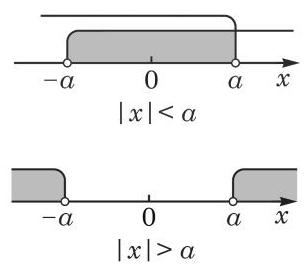
\includegraphics[max width=0.2\textwidth]{images/bo_d7fr3gc91nqc7381iccg_52_195_826_305_273_0.jpg}
\end{center}
\hspace*{3em} 

图 2-2-2

例如,当 \(a > 0\) 时,不等式 \(\left| x\right|  < a \Leftrightarrow   - a < x < a\) ,从而 \(\left| x\right|  < a\) 的解集为 \(\left( {-a,a}\right) ;\left| x\right|  > a \Leftrightarrow  x > a\) 或 \(x <  - a\) ,从而 \(\left| x\right|  > a\) 的解集为 \(\left( {-\infty , - a}\right)  \cup  \left( {a, + \infty }\right)\) (图 2-2-2).

例 14 解不等式 \(\left| {x - 1}\right|  < 2\) .

解 原不等式等价于

\[
- 2 < x - 1 < 2\text{ . }
\]

将上述不等式中的各项同加 1,得 \(- 1 < x < 3\) .

所以，原不等式的解集为 \(\left( {-1,3}\right)\) .

例 15 解不等式 \(\left| {{2x} + 1}\right|  \geq  3\) .

解 原不等式等价于

\[
{2x} + 1 \geq  3\text{ 或 }{2x} + 1 \leq   - 3.
\]

解这两个不等式,得 \(x \geq  1\) 或 \(x \leq   - 2\) .

所以,原不等式的解集为 \(\left( {-\infty , - 2\rbrack \cup \lbrack 1, + \infty }\right)\) .

Q

例 16 解不等式 \(\left| {1 - {2x}}\right|  > x\) .

\HRule

为去掉不等式中的绝对值符号, 先求出方程 \(1 - {2x} = 0\) 的根,再用这个根 \(x = \frac{1}{2}\) 将实数轴划分为两个部分, 分段进行讨论.

\HRule

解 当 \(x > \frac{1}{2}\) 时,原不等式化为 \({2x} - 1 > x\) ,即 \(x > 1\) . 此时, 不等式的解为 \(x > 1\) .

当 \(x \leq  \frac{1}{2}\) 时,原不等式化为 \(1 - {2x} > x\) ,即 \(x < \frac{1}{3}\) . 此时,不等式的解为 \(x < \frac{1}{3}\) .

综上所述,原不等式的解集为 \(\left( {-\infty ,\frac{1}{3}}\right)  \cup  \left( {1, + \infty }\right)\) .

\section*{}



例 17 解不等式 \(\left| {x - 3}\right|  + \left| {x - 5}\right|  < 4\) .

\HRule

为去掉不等式中的两个绝对值符号, 先分别求出方程 \(\left| {x - 3}\right|  = 0\) 及 \(\left| {x - 5}\right|  = 0\) 的根, 再用这两个根 \(x = 3\) 及 \(x = 5\) 将实数轴划分为三个区间，分段进行讨论.

\HRule

解 当 \(x \geq  5\) 时,原不等式化为 \(x - 3 + x - 5 < 4\) ,可解得 \(x < 6\) . 此时,不等式的解为 \(5 \leq  x < 6\) .

当 \(3 \leq  x < 5\) 时,原不等式化为 \(x - 3 + 5 - x < 4\) ,即 \(2 < 4\) , 它始终成立. 此时,不等式的解为 \(3 \leq  x < 5\) .

当 \(x < 3\) 时,原不等式化为 \(3 - x + 5 - x < 4\) ,可解得 \(x > 2\) . 此时，不等式的解为 \(2 < x < 3\) .

综上所述，原不等式的解集为 \(\lbrack 5,6) \cup  \lbrack 3,5) \cup  \left( {2,3}\right)  = \left( {2,6}\right)\) .

\section*{练习 2.2(5)}

解下列不等式:

(1) \(\left| {x + 3}\right|  < 4\) ； (2) \(\left| {1 - {2x}}\right|  > 3\) ；

(3) \(\left| {{2x} - 3}\right|  < {3x} - 2\) ； (4) \(\left| {x + 1}\right|  + \left| {x - 4}\right|  > 7\) .

\section*{习题 2.2}

\section*{A 组}

1. 解下列不等式(组):

(1) \(2\left( {x + 1}\right)  - 3\left( {x - 2}\right)  > 8\) ；

(2) \(\left\{  \begin{array}{l} {3x} - 2\left( {5 - {3x}}\right)  > 8, \\  {2x} \leq  2\left( {{2x} + 3}\right) . \end{array}\right.\)

2. 解下列关于 \(x\) 的不等式:

(1) \({ax} + 4 < {2x} + {a}^{2}\) ，其中 \(a > 2\) ； (2) \({mx} + 1 > x + {m}^{3}\) ，其中 \(m < 1\) ；

(3) \(\left( {p - q}\right) x < {p}^{2} - {q}^{2}\) ，其中 \(p \neq  q\) .

3. 解下列不等式:

(1) \(\left( {x - 2}\right) \left( {3 - x}\right)  \leq  0\) ； (2) \(x\left( {x + 2}\right)  \leq  3\left( {x + 2}\right)\) ；

(3) \(\left( {1 - x}\right) \left( {2 - x}\right)  < 0\) ； (4) \(2\left( {x + 1}\right) \left( {x + 3}\right)  > \left( {x + 3}\right) \left( {x + 4}\right)\) .

4. 设全集为 \(\mathbf{R}\) ,集合 \(A = \left\{  {x \mid  {x}^{2} - {2x} - 3 \geq  0}\right\}  ,B = \left\{  {x \mid  {x}^{2} + x - 2 < 0}\right\}\) . 求:

(1) \(A \cup  B\) ； (2) \(A \cap  B\) ；

(3) \(\overline{A \cap  B}\) ; (4) \(\overline{A} \cup  \overline{B}\) .

5. 已知下列关于 \(x\) 的方程有两个不同实根,求实数 \(k\) 的取值范围:

(1) \({x}^{2} + \left( {k + 3}\right) x + {k}^{2} = 0\) ； (2) \(3{x}^{2} + {2kx} + k = 0\) .

6. 若下列关于 \(x\) 的方程有实数解,求实数 \(k\) 的取值范围:

\section*{}



(1) \({x}^{2} + {kx} - k + 3 = 0\) ； (2) \({x}^{2} + {2\sqrt{2}}x + k\left( {k - 1}\right)  = 0\) .

7. 解下列不等式:

(1) \(\frac{1}{3}{x}^{2} \leq  {2x} - 3\) ； (2) \(4{x}^{2} \geq  {12x} - 9\) ；

(3) \({x}^{2} - x + \frac{1}{4} < 0\) ； (4) \({x}^{2} + \frac{4}{9} > \frac{2}{3}x\) .

8. 解下列不等式:

(1) \({x}^{2} + x + 1 > 0\) ； (2) \(3 - 2\sqrt{2}x \geq   - {x}^{2}\) ；

(3) \(2{x}^{2} + {3x} + 4 < 0\) ； (4) \({x}^{2} \leq  {3x} - 4\) .

9. 已知关于 \(x\) 的一元二次方程 \(2{x}^{2} + {ax} + 1 = 0\) 无实数解,求实数 \(a\) 的取值范围.

10. 已知关于 \(x\) 的一元二次不等式 \({x}^{2} + {ax} + b < 0\) 的解集为 \(\left( {-3, - 1}\right)\) ，求实数 \(a\) 及 \(b\) 的值.

11. 解下列不等式组:

(1) \(\left\{  \begin{array}{l} 6 - x - {x}^{2} \leq  0, \\  {x}^{2} + {3x} - 4 < 0; \end{array}\right.\) (2) \(\left\{  \begin{array}{l} 4{x}^{2} - {27x} + {18} > 0, \\  {x}^{2} - {6x} + 4 < 0; \end{array}\right.\)

(3) \(\left\{  \begin{array}{l} 3{x}^{2} + x - 2 \geq  0, \\  4{x}^{2} - {15x} + 9 > 0. \end{array}\right.\)

12. 解下列不等式:

(1) \(\frac{x + 1}{x - 2} > 0\) ； (2) \(\frac{1}{x} < 1\) ；

(3) \(\frac{2}{3 - {4x}} \geq  1\) ； (4) \(\frac{5}{x + 2} \leq  2\) ；

(5) \(\frac{{4x} + 3}{x - 1} > 5\) .

13. 当关于 \(x\) 的方程 \({4k} - {3x} = 2\left( {k + 2}\right) x\) 的解分别满足以下条件时,求实数 \(k\) 的取值范围.

(1)正数； (2)负数.

14. 解下列不等式:

(1) \(\left| {1 - {4x}}\right|  < 5\) ； (2) \(\left| {x - 4}\right|  < {2x}\) ；

(3) \(\left| {{3x} - 4}\right|  \geq  x + 2\) ； (4) \(\left| {x + 2}\right|  + \left| {x - 3}\right|  < 7\) .

15. 某船从甲码头顺流航行 \({75}\mathrm{\;{km}}\) 到达乙码头,停留 \({30}\mathrm{\;{min}}\) 后再逆流航行 \({126}\mathrm{\;{km}}\) 到达丙码头. 如果水流速度为 \(4\mathrm{\;{km}}/\mathrm{h}\) ,该船要在 \(5\mathrm{\;h}\) 内(包含 \(5\mathrm{\;h}\) )完成整个航行任务，那么船的速度至少要达到多少?

\section*{B 组}

1. 设 \(a\text{ 、 }b \in  \mathbf{R}\) ,解关于 \(x\) 的不等式 \({ax} > b\) .



\section*{}

2. 设 \(a \in  \mathbf{R}\) ,解下列关于 \(x\) 的不等式:

(1) \(\left( {x - a}\right) \left( {x + 3}\right)  \geq  0\) ；

(2) \(\left( {x - a}\right) \left( {x - {2a}}\right)  > 0\) ；

(3) \(x\left( {x - a}\right)  \geq  \left( {a + 1}\right) \left( {x - a}\right)\) .

3. 已知关于 \(x\) 的不等式 \({x}^{2} + {bx} + c > 0\) 的解集是 \(\left( {-\infty ,\frac{1}{2}}\right)  \cup  \left( {2, + \infty }\right)\) ,求实数 \(b\) 及 \(c\) 的值,并求 \({x}^{2} - {bx} + c \leq  0\) 的解集.

4. 解下列不等式:

(1) \(2 < \frac{1}{{3x} - 1} \leq  3\) ；

(2) \(\frac{1}{x} > x\) ；

(3) \(\frac{1}{x - 4} \leq  1 - \frac{x}{4 - x}\) .

5. 解下列不等式:

(1) \(\frac{3{x}^{2} + {2x} + 1}{{x}^{2} + x + 2} \leq  1\) ；\_\_\_\_\_ (2) \(\frac{x - 1}{{x}^{2} - {4x} + 4} \geq  0\) .

6. 解下列不等式:

(1) \(1 < \left| {1 - {2x}}\right|  \leq  7\) ； (2) \(3 < \left| {x - 2}\right|  < 6\) ；

(3) \(\left| {x + 2}\right|  - \left| {3 - {2x}}\right|  < 1\) ； (4) \(\left| \frac{x}{x + 1}\right|  > \frac{x}{x + 1}\) .

7. 若关于 \(x\) 的不等式组 \(\left\{  \begin{array}{l} \left( {{2x} - 3}\right) \left( {{3x} + 2}\right)  \leq  0, \\  x - a > 0 \end{array}\right.\) 没有实数解,求实数 \(a\) 的取值范围.

8. 若关于 \(x\) 的不等式 \({2k}{x}^{2} + {kx} + \frac{1}{8} > 0\) 对于一切实数 \(x\) 都成立,求实数 \(k\) 的取值范围.



\section*{2.3 基本不等式及其应用}

在本章前两节中, 我们学习了一些不等式的性质、求解和证明. 在不等式的应用中, 有一些很基本而十分重要的不等式, 如平均值不等式和三角不等式等, 我们将其统称为基本不等式.

\section*{1 平均值不等式及其应用}

对于正数 \(a\text{ 、 }b\) ,称 \(\frac{a + b}{2}\) 是 \(a\text{ 、 }b\) 的算术平均值 (arithmetic mean),并称 \(\sqrt{ab}\) 是 \(a\text{ 、 }b\) 的几何平均值 (geometric mean). 当 \(a\text{ 、 }b\) 分别表示对同一个量进行两次测量所得的数值时,其算术平均值 \(\frac{a + b}{2}\) 可以理解为这两次测量值的平均. 当 \(a\text{ 、 }b\) 分别表示一个矩形的两边边长时,其几何平均值 \(\sqrt{ab}\) 可以理解为与此矩形面积相同的正方形的边长.

下面的不等式是经典的平均值不等式:

定理(平均值不等式) 两个正数的算术平均值大于等于它们的几何平均值,即对于任意的正数 \(a\text{ 、 }b\) ,有

\[
\frac{a + b}{2} \geq  \sqrt{ab},
\]

且等号当且仅当 \(a = b\) 时成立.

证明 因为

\[
\frac{a + b}{2} - \sqrt{ab} = \frac{{\left( \sqrt{a} - \sqrt{b}\right) }^{2}}{2} \geq  0,
\]

所以

\[
\frac{a + b}{2} \geq  \sqrt{ab},
\]

而且当且仅当 \(\sqrt{a} - \sqrt{b} = 0\) 即 \(a = b\) 时,不等式中等号成立.

\section*{}

\HRule

在 \(a\) 及 \(b\) 有可能为零时, 平均值不等式也显然成立. 因此, 对于任意的非负实数 \(a\text{ 、 }b\) ,平均值不等式都成立.

\HRule

例 1 已知 \(x > 0\) ,求证: \(x + \frac{1}{x} \geq  2\) ,并指出等号成立的条件.

证明 因为 \(x > 0\) ,由平均值不等式,得

\[
x + \frac{1}{x} \geq  2\sqrt{x \cdot  \frac{1}{x}} = 2,
\]

且等号只有当 \(x = \frac{1}{x}\) ,即 \({x}^{2} = 1\) 时才成立. 由于 \(x > 0\) ,因此 \(x = 1\) .

所以,当且仅当 \(x = 1\) 时, \(x + \frac{1}{x} = 2\) .

例 2 已知 \({ab} > 0\) ,求证: \(\frac{b}{a} + \frac{a}{b} \geq  2\) ,并指出等号成立的条件.

证明 因为 \({ab} > 0\) ,所以 \(a\text{ 、 }b\) 同号,因而 \(\frac{b}{a} > 0,\frac{a}{b} > 0\) .

由平均值不等式, 得

\[
\frac{b}{a} + \frac{a}{b} \geq  2\sqrt{\frac{b}{a} \cdot  \frac{a}{b}} = 2,
\]

且等号当且仅当 \(\frac{b}{a} = \frac{a}{b}\) ,即 \(a = b\) 时才成立.

除了平均值不等式, 还有一些常用的不等式.

定理 对于任意的实数 \(a\text{ 、 }b\) ,有

\[
{\left( \frac{a + b}{2}\right) }^{2} \geq  {ab}
\]

且等号当且仅当 \(a = b\) 时成立.

证明 对任意给定的实数 \(a\text{ 、 }b\) ,总有 \({a}^{2} + {b}^{2} \geq  {2ab}\) ,且等号当且仅当 \(a = b\) 时成立. 于是

\[
{a}^{2} + {b}^{2} + {2ab} \geq  {4ab},
\]

从而

\[
{\left( a + b\right) }^{2} \geq  {4ab},
\]

即

\[
{\left( \frac{a + b}{2}\right) }^{2} \geq  {ab}
\]

从而原不等式成立,且等号当且仅当 \(a = b\) 时成立.

包括平均值不等式在内的上述一些不等式常常可被应用





于对一些量做估计, 特别是可用于求解一些最大值或最小值问题.

例 3 设 \(x \in  \mathbf{R}\) ,求二次函数 \(y = x\left( {4 - x}\right)\) 的最大值.

解 由不等式 \({\left( \frac{a + b}{2}\right) }^{2} \geq  {ab}\) ,推得

\[
x\left( {4 - x}\right)  \leq  {\left( \frac{x + 4 - x}{2}\right) }^{2} = 4.
\]

于是,当 \(x = 4 - x\) ,即 \(x = 2\) 时, \(y\) 取得最大值 4 .

\section*{练习 2.3(1)}

1. 设 \(a\) 是正数,求证: \(a + 1 \geq  2\sqrt{a}\) .

2. 证明: 若 \(x < 0\) ,则 \(x + \frac{1}{x} \leq   - 2\) ,并指出等号成立的条件.

例 4 设 \(a\text{ 、 }b\) 为正数,且 \(a + {2b} = 1\) ,比较 \({ab}\) 的值与 \(\frac{1}{8}\) 的大小.

解 因为

\[
{ab} = \frac{1}{2}\left( {a \cdot  {2b}}\right)  \leq  \frac{1}{2}{\left( \frac{a + {2b}}{2}\right) }^{2} = \frac{1}{8},
\]

所以 \({ab} \leq  \frac{1}{8}\) ,当且仅当 \(a = {2b}\) 且 \(a + {2b} = 1\) ,即 \(a = \frac{1}{2}\) 且 \(b = \frac{1}{4}\) 时,才有 \({ab} = \frac{1}{8}\) ; 而在其他情形,均有 \({ab} < \frac{1}{8}\) .

例 5 证明:

(1)在周长为常数的所有矩形中,正方形的面积最大;

(2)在面积相同的所有矩形中,正方形的周长最小.

证明 (1) 设矩形的周长为常数 \(l\left( {l > 0}\right)\) ,而其长、宽分别为 \(x\text{ 、 }y\left( {x > 0,y > 0}\right)\) ,就有 \({2x} + {2y} = l\) . 此矩形的面积为 \(S = {xy}\) . 由平均值不等式,有

\[
S = {xy} \leq  {\left( \frac{x + y}{2}\right) }^{2} = {\left( \frac{l}{4}\right) }^{2},
\]

当且仅当 \(x = y = \frac{l}{4}\) ,即矩形为正方形时,面积 \(S\) 取得最大值 \(\frac{{l}^{2}}{16}\) .

(2)设矩形的面积为常数 \(S\left( {S > 0}\right)\) ，而其长、宽仍分别设为 \(x\text{ 、 }y\left( {x > 0,y > 0}\right)\) ,就有 \({xy} = S\) . 此矩形的周长为 \(l = 2\left( {x + y}\right)\) .

\section*{}

由平均值不等式, 有

\[
\frac{x + y}{2} \geq  \sqrt{xy} = \sqrt{S}.
\]

所以, \(l = 2\left( {x + y}\right)  \geq  4\sqrt{S}\) ,且当且仅当 \(x = y = \sqrt{S}\) ,即矩形为正方形时,周长 \(l\) 取最小值 \(4\sqrt{S}\) .

由例 5 可知,根据平均值不等式 \(\sqrt{xy} \leq  \frac{x + y}{2}\left( {x > 0,y > 0}\right)\) , 当乘积 \({xy}\) 为定值时,和 \(x + y\) 有最小值; 而当和 \(x + y\) 为定值时,乘积 \({xy}\) 有最大值. 此外,当且仅当 \(x = y\) 时,才取得相应的最小值或最大值.

例 6 某新建居民小区欲建一面积为 \({700}{\mathrm{\;m}}^{2}\) 的矩形绿地, 并在绿地四周铺设人行道. 设计要求绿地外南北两侧人行道宽 \(3\mathrm{\;m}\) ,东西两侧人行道宽 \(4\mathrm{\;m}\) ,如图 2-3-1 所示 (图中单位: \(\mathrm{m}\) ). 问如何设计绿地的边长, 才能使人行道的占地面积最小. (结果精确到 \({0.1}\mathrm{\;m}\) )

\begin{center}
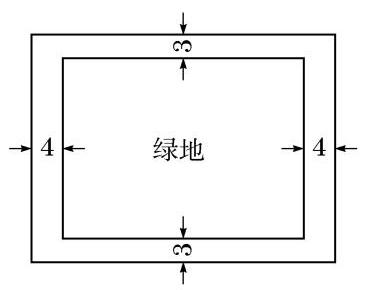
\includegraphics[max width=0.3\textwidth]{images/bo_d7fr3gc91nqc7381iccg_59_1120_797_365_290_0.jpg}
\end{center}
\hspace*{3em} 

图 2-3-1

解 设矩形绿地的南北侧边长为 \(x\mathrm{\;m}\) ,则其东西侧边长为 \(\frac{700}{x}\mathrm{\;m}\) ,人行道的占地面积 \(\left( {\text{ 记为 }S\left( {\mathrm{\;m}}^{2}\right) }\right)\) 为

\[
\left( {x + 8}\right) \left( {\frac{700}{x} + 6}\right)  - {700},
\]

即

\[
S = {6x} + \frac{5600}{x} + {48}.
\]

利用平均值不等式，有

\[
{6x} + \frac{5600}{x} \geq  2\sqrt{{6x} \cdot  \frac{5600}{x}} = 2\sqrt{33600} = {80}\sqrt{21},
\]

且当且仅当 \({6x} = \frac{5600}{x}\) ,即 \(x = {20}\sqrt{\frac{7}{3}} \approx  {30.6}\left( \mathrm{\;m}\right)\) 时, \(S\) 达到最小值 \({48} + {80}\sqrt{21}\left( {\mathrm{\;m}}^{2}\right)\) ,此时 \(\frac{700}{x} \approx  {22.9}\left( \mathrm{\;m}\right)\) .

所以，当设计绿地的南北侧边长约为 \({30.6}\mathrm{\;m}\) ，东西侧边长约为 \({22.9}\mathrm{\;m}\) 时,人行道的占地面积最小.

\section*{练习2.3(2)}

1. 用一根长为 \(l\) 的铁丝制成一个矩形框架. 当长和宽分别为多少时,该框架的面积



\section*{}

最大?

2. 在面积为 \(\pi\) 的圆中作一个内接矩形,使它的面积最大. 求此矩形面积的最大值及此时矩形的各边长.

\section*{2 三角不等式}

在后续向量、复数等内容的学习中, 下述三角不等式将起着重要的作用, 且其几何意义将十分明显.

Q

\HRule

这个不等式与三角形两边之和大于第三边相似, 故称为三角不等式(triangle inequality).

\HRule

定理(三角不等式) 两个实数和的绝对值小于等于它们绝对值的和,即对于任意给定的实数 \(a\text{ 、 }b\) ,有

\[
\left| {a + b}\right|  \leq  \left| a\right|  + \left| b\right| ,
\]

且等号当且仅当 \({ab} \geq  0\) 时成立.

?

证明 因为 \(\left| {a + b}\right|  \leq  \left| a\right|  + \left| b\right|\) 等价于

\[
{\left| a + b\right| }^{2} \leq  {\left( \left| a\right|  + \left| b\right| \right) }^{2},
\]

\HRule

请通过讨论 \(a\text{ 、 }b\) 的符号证明三角不等式.

\HRule

即 \({a}^{2} + {2ab} + {b}^{2} \leq  {a}^{2} + 2\left| {ab}\right|  + {b}^{2}\) ,也即 \({2ab} \leq  2\left| {ab}\right|\) ,所以三角不等式成立,且等号当且仅当 \({ab} \geq  0\) 时成立.

例 7 已知 \(a\text{ 、 }b\) 为实数，求证: \(\left| {a + b}\right|  + \left| {a - b}\right|  \geq  2\left| a\right|\) .

证明 因为 \(\left( {a + b}\right)  + \left( {a - b}\right)  = {2a}\) ,由三角不等式,有

\[
\left| {\left( {a + b}\right)  + \left( {a - b}\right) }\right|  \leq  \left| {a + b}\right|  + \left| {a - b}\right| ,
\]

即

\[
\left| {2a}\right|  \leq  \left| {a + b}\right|  + \left| {a - b}\right| ,
\]

所以

\[
\left| {a + b}\right|  + \left| {a - b}\right|  \geq  2\left| a\right| .
\]

例 8 已知 \(a\text{ 、 }b\) 为实数，求证: \(\left| a\right|  - \left| b\right|  \leq  \left| {a - b}\right|\) ，并指出等号成立的条件.

证明 \(\left| a\right|  - \left| b\right|  \leq  \left| {a - b}\right|\) 等价于 \(\left| a\right|  \leq  \left| {a - b}\right|  + \left| b\right|\) . 由三角不等式, 有

\[
\left| {a - b}\right|  + \left| b\right|  \geq  \left| {\left( {a - b}\right)  + b}\right|  = \left| a\right| ,
\]

所以

\[
\left| a\right|  - \left| b\right|  \leq  \left| {a - b}\right| ,
\]

且等号当且仅当 \(\left( {a - b}\right) b \geq  0\) ,即 \({ab} \geq  {b}^{2}\) 时成立.

例 9 证明: \(\left| {x - 3}\right|  + \left| {x - 5}\right|  \geq  2\) 对所有实数 \(x\) 恒成立,



\section*{}

并求等号成立时 \(x\) 的取值范围.

证明 因为 \(\left| {x - 5}\right|  = \left| {5 - x}\right|\) ,由三角不等式,有

\[
\left| {x - 3}\right|  + \left| {x - 5}\right|  = \left| {x - 3}\right|  + \left| {5 - x}\right|  \geq  \left| {x - 3 + 5 - x}\right|  = 2,
\]

所以

\[
\left| {x - 3}\right|  + \left| {x - 5}\right|  \geq  2,
\]

且等号当且仅当 \(\left( {x - 3}\right) \left( {5 - x}\right)  \geq  0\) ,即 \(\left( {x - 3}\right) \left( {x - 5}\right)  \leq  0\) 时成立.

因此， \(\left| {x - 3}\right|  + \left| {x - 5}\right|  \geq  2\) 对所有实数 \(x\) 恒成立，且当且仅当 \(x \in  \left\lbrack  {3,5}\right\rbrack\) 时，等号成立.

\section*{练习 2.3(3)}

1. 已知 \(a\text{ 、 }b \in  \mathbf{R}\) . 求证: \(\left| {a + b}\right|  + \left| {a - b}\right|  \geq  2\left| b\right|\) .

2. 已知实数 \(a\text{ 、 }b\) 满足 \(\left| a\right|  < \frac{1}{2},\left| b\right|  < \frac{1}{2}\) . 证明下列各式:

(1) \(\left| {a + b}\right|  < 1\) ； (2) \(\left| {a - b}\right|  < 1\) .

\section*{习题 2.3}

\section*{A 组}

1. 如果实数 \(a\text{ 、 }b\) 同号,那么下列命题中正确的是 ( )

A. \({a}^{2} + {b}^{2} > {2ab}\) ; B. \(a + b \geq  2\sqrt{ab}\) ;

C. \(\frac{1}{a} + \frac{1}{b} > \frac{2}{\sqrt{ab}}\) ; D. \(\frac{b}{a} + \frac{a}{b} \geq  2\) .

2. 设 \(a > b > 0\) ,将四个正数 \(a\text{ 、 }b\text{ 、 }\sqrt{ab}\text{ 、 }\frac{a + b}{2}\) 按从小到大的顺序排列,并说明理由.

3. 已知 \(a\text{ 、 }b\) 为正数,求证: \(\frac{2}{\frac{1}{a} + \frac{1}{b}} \leq  \sqrt{ab}\) ,并指出等号的成立条件.

4. 设 \(a\text{ 、 }b \in  \mathbf{R}\) ,求证: \({a}^{2} + 2{b}^{2} + 1 \geq  {2b}\left( {a + 1}\right)\) .

5. 设 \(x \in  \mathbf{R}\) ,求二次函数 \(y = \left( {x - 1}\right) \left( {5 - x}\right)\) 的最大值.

6. 已知直角三角形斜边长等于 \({10}\mathrm{\;{cm}}\) ,求直角三角形面积的最大值.

7. 已知 \(a\text{ 、 }b\text{ 、 }c\) 为实数,求证: \(\left| {a - b}\right|  \leq  \left| {a - c}\right|  + \left| {c - b}\right|\) .

8. 设 \(x \in  \mathbf{R}\) ,求方程 \(\left| {x - 2}\right|  + \left| {{2x} - 3}\right|  = \left| {{3x} - 5}\right|\) 的解集.

\section*{}



B 组

1. 设 \(0 < a < b\) ,且 \(a + b = 1\) ,请将 \(a\text{ 、 }b\text{ 、 }\frac{1}{2}\text{ 、 }{2ab}\text{ 、 }{a}^{2} + {b}^{2}\) 从小到大排列,并说明理由.

2. 已知 \(a\) 为正数,比较 \(\frac{{a}^{2} + {2a} + 1}{a}\) 的值与 4 的大小.

3. 已知 \(a\text{ 、 }b\) 为正数,求证: \(\left( {a + b}\right) \left( {\frac{1}{a} + \frac{1}{b}}\right)  \geq  4\) .

4. 已知 \(a\text{ 、 }b\) 是互不相等的正数,求证: \(\left( {{a}^{2} + 1}\right) \left( {{b}^{2} + 1}\right)  > {4ab}\) .

5. 证明: 对于正数 \(h\) ,如果 \(\left| {x - a}\right|  < \frac{h}{2},\left| {y - a}\right|  < \frac{h}{2}\) ,那么 \(\left| {x - y}\right|  < h\) .

6. 已知直角坐标平面上的三点 \(A\left( {{x}_{1},{y}_{1}}\right)\) 、 \(B\left( {{x}_{2},{y}_{2}}\right)\) 、 \(C\left( {{x}_{3},{y}_{3}}\right)\) ,记

\[
d\left( {A,B}\right)  = \left| {{x}_{2} - {x}_{1}}\right|  + \left| {{y}_{2} - {y}_{1}}\right| ,
\]

\[
d\left( {B,C}\right)  = \left| {{x}_{3} - {x}_{2}}\right|  + \left| {{y}_{3} - {y}_{2}}\right| ,
\]

\[
d\left( {C,A}\right)  = \left| {{x}_{1} - {x}_{3}}\right|  + \left| {{y}_{1} - {y}_{3}}\right| .
\]

求证: \(d\left( {A,B}\right)  \leq  d\left( {B,C}\right)  + d\left( {C,A}\right)\) .

7. 已知 \(a\text{ 、 }b\text{ 、 }c\) 是实数,求证: \(\left| {a + b + c}\right|  \leq  \left| a\right|  + \left| b\right|  + \left| c\right|\) .

8. 证明: \(\left| {x + 2}\right|  - \left| {x - 1}\right|  \geq   - 3\) ,对所有实数 \(x\) 均成立,并求等号成立时 \(x\) 的取值范围.

\section*{探究与实践}

\section*{利用等式证明不等式}

下图(图 2-3-2)称为弦图，是我国古代三国时期的数学家赵爽为《周髀算经》作注时为证明勾股定理所绘制. 此图曾作为 2002 年在北京召开的第 24 届国际数学家大会的会标. (图 2-3-3)

\begin{center}
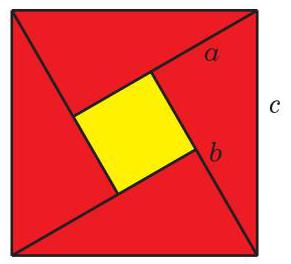
\includegraphics[max width=0.2\textwidth]{images/bo_d7fr3gc91nqc7381iccg_62_444_1796_291_264_0.jpg}
\end{center}
\hspace*{3em} 

图 2-3-2

\begin{center}

\includegraphics[max width=0.2\textwidth]{images/bo_d7fr3gc91nqc7381iccg_62_948_1672_287_385_0.jpg}
\end{center}
\hspace*{3em} 

图 2-3-3





赵爽运用图形割补后面积不变的原理, 通过构造相应的几何图形来证明勾股定理. “按弦图，又可以勾股相乘为朱实二，倍之为朱实四，以勾股之差自相乘为中黄实，加差实,亦成弦实.” 其证明过程可用字母表示为 \(4 \times  \frac{1}{2}{ab} + {\left( a - b\right) }^{2} = {c}^{2}\) ,化简即得勾股定理 \({a}^{2} + {b}^{2} = {c}^{2}.\)

弦图不仅能用于证明等式, 也能用于证明不等式. 事实上, 利用弦图得到的等式 \({2ab} + {\left( a - b\right) }^{2} = {a}^{2} + {b}^{2}\) ,可推出: \({a}^{2} + {b}^{2} \geq  {2ab}\) ,且等号当且仅当 \(a = b\) 时成立.

运用这样的想法,我们可以由等式出发证明一些不等式. 例如,容易证明 \(\left( {a + b + c}\right) \; \left\lbrack  {{\left( a - b\right) }^{2} + {\left( b - c\right) }^{2} + {\left( c - a\right) }^{2}}\right\rbrack   = 2\left( {{a}^{3} + {b}^{3} + {c}^{3} - {3abc}}\right)\) 成立. 由此,可以推出: 对于非负实数 \(a\text{ 、 }b\text{ 、 }c\) ,有 \({a}^{3} + {b}^{3} + {c}^{3} \geq  {3abc}\) ,且等号当且仅当 \(a = b = c\) 时成立. 又如,由 \(\left( {{a}^{2} + }\right. \; \left. {b}^{2}\right) \left( {{x}^{2} + {y}^{2}}\right)  = {\left( ax + by\right) }^{2} + {\left( ay - bx\right) }^{2}\) ,可以推得: \(\left( {{a}^{2} + {b}^{2}}\right) \left( {{x}^{2} + {y}^{2}}\right)  \geq  {\left( ax + by\right) }^{2}\) ,且等号当且仅当 \({ay} = {bx}\) 时成立.

请仿照上述例子,计算 \(\left( {{a}^{2} + {b}^{2} + {c}^{2}}\right) \left( {{x}^{2} + {y}^{2} + {z}^{2}}\right)  - {\left( ax + by + cz\right) }^{2}\) ,并看由此能否得到一个相应的不等式.

\section*{课后阅读}

\section*{平均值不等式的应用}

船速一定的汽船，在静水中和有流速的河中往返航行同样的距离，所需的时间是否一样? 有人认为二者所需的时间是一样的, 他们的理由是: 当河水有流速时, 汽船逆流上行虽然速度要减慢，但回来时顺流下行的速度要加快，二者互相补偿，航行时间就应和在静水中往返一次所需的时间一样.

上面的说法貌似有理，但事实却并非如此. 为说明这一点，只需做一下简单的计算就可以了. 设汽船在静水中航行的速度为 \({v}_{\text{ 静 }}\) ,河水的流速为 \({v}_{\text{ 水 }}\) ,汽船在河流中航行的单程距离为 \(L\) . 那么汽船逆流上行的实际速度是 \({v}_{\mathrm{\text{ 上 }}} = {v}_{\text{ 静 }} - {v}_{\text{ 水 }}\) ,而顺流下行的实际速度是 \({v}_{\mathrm{\text{ 下 }}} = {v}_{\text{ 静 }} + {v}_{\text{ 水 }}\) . 这样汽船往返一次所需的总时间是

\[
\frac{L}{{v}_{\mathrm{L}}} + \frac{L}{{v}_{\mathrm{T}}} = \frac{L}{{v}_{\mathrm{\text{ 静 }}} - {v}_{\mathrm{\text{ 水 }}}} + \frac{L}{{v}_{\mathrm{\text{ 静 }}} + {v}_{\mathrm{\text{ 水 }}}} = \frac{{2L}{v}_{\mathrm{\text{ 静 }}}}{{v}_{\mathrm{\text{ 静 }}}^{2} - {v}_{\mathrm{\text{ 水 }}}^{2}} = \frac{2L}{{v}_{\mathrm{\text{ 静 }}}\left( {1 - \frac{{v}_{\mathrm{\text{ 水 }}}^{2}}{{v}_{\mathrm{\text{ 静 }}}^{2}}}\right) },
\]

它总是大于汽船在静水中往返一次的时间 \(\frac{2L}{{v}_{\text{ 静 }}}\) ，且河水流速愈大，二者的差距愈大.

由上式, 我们可以看到, 汽船在有流速的河中行驶的平均速度是

\[
\frac{2L}{\frac{L}{{v}_{\mathrm{\text{ 上 }}}} + \frac{L}{{v}_{\mathrm{\text{ 下 }}}}} = \frac{2}{\frac{1}{{v}_{\mathrm{\text{ 上 }}}} + \frac{1}{{v}_{\mathrm{\text{ 下 }}}}},
\]

它也是汽船上、下航行速度 \({v}_{\text{ 上 }}\text{ 、 }{v}_{\text{ 下 }}\) 的某种平均值,称为调和平均值. 而汽船上、下航行速度 \({v}_{\text{ 上 }}\text{ 、 }{v}_{\text{ 下 }}\) 的算术平均值

\[
\frac{{v}_{\text{ 上 }} + {v}_{\text{ 下 }}}{2} = {v}_{\text{ 静 }}
\]

正是汽船在静水中航行的速度. 注意到

\[
\frac{2}{\frac{1}{{v}_{\mathrm{\text{ 上 }}}} + \frac{1}{{v}_{\mathrm{\text{ 下 }}}}} = {v}_{\text{ 静 }}\left( {1 - \frac{{v}_{\text{ 水 }}^{2}}{{v}_{\text{ 静 }}^{2}}}\right)  \leq  {v}_{\text{ 静 }} = \frac{{v}_{\mathrm{\text{ 上 }}} + {v}_{\mathrm{\text{ 下 }}}}{2},
\]

就说明调和平均值总小于等于算术平均值.

事实上,对此有一个一般性的结论: 对任意给定的两个正数 \(a\text{ 、 }b\) ,已知 \(\frac{a + b}{2}\) 为其算术平均值,并定义 \(\frac{2}{\frac{1}{a} + \frac{1}{b}}\) 为其调和平均值 (harmonic mean),就有

\[
\frac{2}{\frac{1}{a} + \frac{1}{b}} \leq  \frac{a + b}{2}
\]

且等号当且仅当 \(a = b\) 时成立,即调和平均值必小于等于算术平均值.

迈克耳孙-莫雷实验(1887 年)是历史上著名的实验. 过去人们认为光既然是一种波， 而波的传播是需要媒介的，如声波的传播需要空气做媒介，水波的传播需要水做媒介等， 因此光的传播也需要有媒介. 但光是能够在真空中传播的, 因此人们想象整个宇宙空间 (包括真空)中充满了一种作为光传播媒介的神秘物质——以太. 当地球以 \(v = {30}\mathrm{\;{km}}/\mathrm{s}\) 的速度绕太阳运动时,必定会有强烈的“以太风”迎面吹来. 如果用 \(c\) 表示光速,那么光线迎 ”以太风”传播一定距离 \(L\) 再反射回来所花费的时间是 \(\frac{L}{c + v} + \frac{L}{c - v}\) ,而光线垂直于 “以太风”方向传播同样的距离再反射回来所花费的时间易见为 \(\frac{2L}{\sqrt{{c}^{2} - {v}^{2}}} = 2\sqrt{\frac{L}{c + v} \cdot  \frac{L}{c - v}}\) . 根据平均值不等式,当 \(v \neq  0\) 时,成立 \(\frac{L}{c + v} + \frac{L}{c - v} > 2\sqrt{\frac{L}{c + v} \cdot  \frac{L}{c - v}}\) .

迈克耳孙(A. Michelson)和莫雷(E. Morley)设计了一个实验来测量上述两者的差，结果是零. 这证明了以太根本就不存在. 随着爱因斯坦相对论的建立, 以太学说逐渐被学界抛弃.

1907 年, 迈克耳孙因 “发明光学干涉仪并使用其进行光谱学和基本度量学研究”, 获得了诺贝尔物理学奖. 作为迈克耳孙光学干涉仪的一个最著名的应用, 迈克耳孙-莫雷实验解决了当年普遍困惑物理学界的问题, 而其基本思想和平均值不等式这一初等数学的知识有关!

\section*{内容提要}

1. 实数大小的比较:

\(a > b \Leftrightarrow  a - b > 0;a = b \Leftrightarrow  a - b = 0;a < b \Leftrightarrow  a - b < 0\) .

2. 等式的基本性质:

传递性 如果 \(a = b\) ，且 \(b = c\) ，那么 \(a = c\) .

加法性质 如果 \(a = b,c \in  \mathbf{R}\) ,那么 \(a + c = b + c\) .

乘法性质 如果 \(a = b,c \in  \mathbf{R}\) ,那么 \({ac} = {bc}\) .

3. 不等式的基本性质:

传递性 如果 \(a > b\) ，且 \(b > c\) ，那么 \(a > c\) .

加法性质 如果 \(a > b,c \in  \mathbf{R}\) ，那么 \(a + c > b + c\) .

乘法性质 如果 \(a > b,c > 0\) ,那么 \({ac} > {bc}\) ; 如果 \(a > b,c < 0\) ,那么 \({ac} < {bc}\) .

4. 不等式的常用性质:

如果 \(a > b,c > d\) ,那么 \(a + c > b + d\) .

如果 \(a > b > 0\) ,那么 \(\frac{1}{b} > \frac{1}{a} > 0\) .

如果 \(a > b > 0,c > d > 0\) ,那么 \({ac} > {bd} > 0\) .

如果 \(a > b > 0\) ,那么 \({a}^{n} > {b}^{n} > 0\) ,其中 \(n\) 是正整数.

如果 \({a}^{n} > {b}^{n} > 0\) ,其中 \(a > 0,b > 0,n\) 是正整数,那么 \(a > b > 0\) .

5. 一元二次方程的根与系数关系:

设 \(a{x}^{2} + {bx} + c = 0\left( {a \neq  0}\right)\) 的两根为 \({x}_{1}\text{ 、 }{x}_{2}\) ,则 \({x}_{1} + {x}_{2} =  - \frac{b}{a},{x}_{1}{x}_{2} = \frac{c}{a}\) .

6. 一元二次不等式的求解(下表中均假设 \(a > 0\) ，而 \(\Delta  = {b}^{2} - {4ac}\) ):

\begin{center}
\adjustbox{max width=\textwidth}{
\begin{tabular}{|c|c|c|c|}
\hline
\phantom{X} & \(\Delta  > 0\) & \(\Delta  = 0\) & \(\Delta  < 0\) \\
\cline{1-4}
\(a{x}^{2} + {bx} + c = 0\) & 有两不同实根 \({x}_{1} < {x}_{2}\) & 有两相同实根 \({x}_{1} = {x}_{2}\) & 无实根 \\
\cline{1-4}
\(a{x}^{2} + {bx} + c > 0\) & 解集为 \(\left( {-\infty ,{x}_{1}}\right)  \cup  \left( {{x}_{2}, + \infty }\right)\) & 解集为 \(\left( {-\infty ,{x}_{1}}\right)  \cup  \left( {{x}_{1}, + \infty }\right)\) & 解集为 R \\
\cline{1-4}
\(a{x}^{2} + {bx} + c \geq  0\) & 解集为 \(\left( {-\infty ,{x}_{1}}\right\rbrack   \cup  \left\lbrack  {{x}_{2}, + \infty }\right)\) & 解集为 \(\mathbf{R}\) & 解集为 R \\
\cline{1-4}
\(a{x}^{2} + {bx} + c < 0\) & 解集为 \(\left( {{x}_{1},{x}_{2}}\right)\) & 解集为 \(\varnothing\) & 解集为 \(\varnothing\) \\
\cline{1-4}
\(a{x}^{2} + {bx} + c \leq  0\) & 解集为 \(\left\lbrack  {{x}_{1},{x}_{2}}\right\rbrack\) & 解集为 \(\left\{  {x}_{1}\right\}\) & 解集为 \(\varnothing\) \\
\cline{1-4}
\hline
\end{tabular}
}
\end{center}



7. 基本不等式:

平均值不等式 \(\frac{a + b}{2} \geq  \sqrt{ab}\left( {a > 0,b > 0}\right)\) ，当且仅当 \(a = b\) 时等号成立.

常用不等式 \({a}^{2} + {b}^{2} \geq  {2ab}\) ,当且仅当 \(a = b\) 时等号成立.

\[
{\left( \frac{a + b}{2}\right) }^{2} \geq  {ab}\text{ ,当且仅当 }a = b\text{ 时等号成立. }
\]

三角不等式 \(\left| {a + b}\right|  \leq  \left| a\right|  + \left| b\right|\) ，当且仅当 \({ab} \geq  0\) 时等号成立.

\section*{复习题}

\section*{A 组}

1. 设一元二次方程 \(2{x}^{2} - {6x} - 3 = 0\) 的两个实根为 \({x}_{1}\text{ 、 }{x}_{2}\) ,求下列各式的值:

(1) \(\left( {{x}_{1} + 1}\right) \left( {{x}_{2} + 1}\right)\) ； (2) \(\left( {{x}_{1}^{2} - 1}\right) \left( {{x}_{2}^{2} - 1}\right)\) .

2. 设 \(a > b > 0\) ,比较 \(\frac{b + {2a}}{a + {2b}}\) 与 \(\frac{a}{b}\) 的值的大小.

3. 已知 \(x > y\) ,求证: \({x}^{3} - {y}^{3} > {x}^{2}y - x{y}^{2}\) .

4. 若关于 \(x\) 的不等式 \(\left( {a + 1}\right) x - a < 0\) 的解集为 \(\left( {2, + \infty }\right)\) ,求实数 \(a\) 的值,并求不等式 \(\left( {a - 1}\right) x + 3 - a > 0\) 的解集.

5. 解下列一元二次不等式:

(1) \(- {x}^{2} + {11} <  - {2x} - 4\) ； (2) \(3{x}^{2} < {13x} + {10}\) ；

(3) \({6x} + 2 \geq  5{x}^{2}\) ； (4) \({x}^{2} \leq  8\left( {1 - x}\right)\) ；

(5) \(- {x}^{2} \geq  9\left( {9 - {2x}}\right)\) ； (6) \(3\left( {x - 3}\right)  \leq  {x}^{2}\) .

6. 试写出一个二次项系数为 1 的一元二次不等式, 使它的解集分别为:

(1) \(\left( {-\infty ,\sqrt{2}}\right)  \cup  \left( {\sqrt{2}, + \infty }\right)\) ； (2) \(\left\lbrack  {2 - \sqrt{3},2 + \sqrt{3}}\right\rbrack\) .

7. 求不等式 \(5 \leq  {x}^{2} - {2x} + 2 < 2\) \_6 的所有正整数解.

8. 解下列分式不等式:

(1) \(\frac{{2x} + 1}{x + 7} >  - 3\) ； (2) \(\frac{3x}{{x}^{2} + 2} \geq  1\) .

9. 设关于 \(x\) 的不等式 \({a}_{1}{x}^{2} + {b}_{1}x + {c}_{1} > 0\) 与 \({a}_{2}{x}^{2} + {b}_{2}x + {c}_{2} > 0\) 的解集分别为 \(A\text{ 、 }B\) , 试用集合运算表示下列不等式组的解集:

(1) \(\left\{  \begin{array}{l} {a}_{1}{x}^{2} + {b}_{1}x + {c}_{1} > 0, \\  {a}_{2}{x}^{2} + {b}_{2}x + {c}_{2} > 0; \end{array}\right.\)

\section*{}

(2) \(\left\{  \begin{array}{l} {a}_{1}{x}^{2} + {b}_{1}x + {c}_{1} \leq  0, \\  {a}_{2}{x}^{2} + {b}_{2}x + {c}_{2} > 0; \end{array}\right.\)

(3) \(\left\{  \begin{array}{l} {a}_{1}{x}^{2} + {b}_{1}x + {c}_{1} \leq  0, \\  {a}_{2}{x}^{2} + {b}_{2}x + {c}_{2} \leq  0. \end{array}\right.\)

10. 解下列含绝对值的不等式:

(1) \(\left| {{2x} - 1}\right|  \leq  x\) ； (2) \(\left| {{2x} + 1}\right|  + \left| {x - 2}\right|  < 8\) .

11. 已知 \(a\text{ 、 }b\) 是正数,求证: \(\sqrt{\left( {1 + a}\right) \left( {1 + b}\right) } \geq  1 + \sqrt{ab}\) .

12. 如图,在直角三角形 \({ABC}\) 中, \({AD}\) 垂直于斜边 \({BC}\) ,且垂足为 \(D\) . 设 \({BD}\) 及 \({CD}\) 的长度分别为 \(a\) 与 \(b\) .

(1)求斜边上的高 \({AD}\) 与中线 \({AE}\) 的长；

(2)用不等式表示斜边上的高 \({AD}\) 与中线 \({AE}\) 长度的大小关系.

\begin{center}
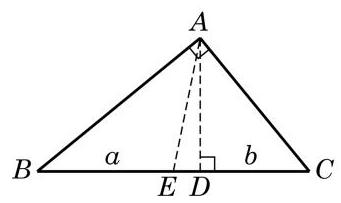
\includegraphics[max width=0.2\textwidth]{images/bo_d7fr3gc91nqc7381iccg_67_316_996_341_203_0.jpg}
\end{center}
\hspace*{3em} 

(第 12 题)

\begin{center}
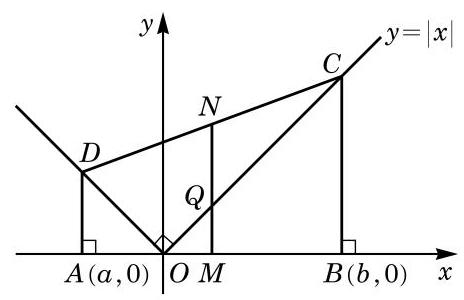
\includegraphics[max width=0.3\textwidth]{images/bo_d7fr3gc91nqc7381iccg_67_836_906_464_300_0.jpg}
\end{center}
\hspace*{3em} 

(第 13 题)

13. 如图,已知直角梯形 \({ABCD}\) 的顶点 \(A\left( {a,0}\right) \text{ 、 }B\left( {b,0}\right)\) 位于 \(x\) 轴上,顶点 \(C\text{ 、 }D\) 落在函数 \(y = \left| x\right|\) 的图像上， \(M\text{ 、 }N\) 分别为线段 \({AB}\text{ 、 }{CD}\) 的中点， \(O\) 为坐标原点， \(Q\) 为线段 \({OC}\) 与线段 \({MN}\) 的交点.

(1)求中点 \(M\) 的坐标，以及线段 \({MQ}\) 、 \({MN}\) 的长度；

(2)用不等式表示 \({MQ}\) 、 \({MN}\) 长度的大小关系.

\section*{B 组}

1. 已知一元二次方程 \({x}^{2} + {px} + p = 0\) 的两个实根分别为 \(\alpha\) 、 \(\beta\) ，且 \({\alpha }^{2} + {\beta }^{2} = 3\) . 求实数 \(p\) 的值.

2. 已知一元二次方程 \(2{x}^{2} - {4x} + m + 3 = 0\) 有两个同号实根,求实数 \(m\) 的取值范围.

3. 设 \(a\text{ 、 }b \in  \mathbf{R}\) ,已知关于 \(x\) 的不等式 \(\left( {a + b}\right) x + \left( {b - {2a}}\right)  < 0\) 的解集为 \(\left( {1, + \infty }\right)\) , 求不等式 \(\left( {a - b}\right) x + {3b} - a > 0\) 的解集.

4. 解下列不等式:

(1) \(- 2 < \frac{1}{{2x} + 1} \leq  3\) ； (2) \(2 < \left| {x + 1}\right|  \leq  3\) .

5. 已知集合 \(A = \{ x \mid  \left| {x - a}\right|  < 2\} ,B = \left\{  {x\left| {\;\frac{{2x} - 1}{x + 2} < 1}\right. }\right\}\) ，且 \(A \subseteq  B\) . 求实数 \(a\) 的取值范围.

6. 证明: 若 \(x >  - 1\) ,则 \(x + \frac{1}{x + 1} \geq  1\) ,并指出等号成立的条件.

7. 设 \(a\text{ 、 }b\) 为正数,且 \(a + b = 2\) . 求 \(\frac{1}{a} + \frac{1}{b}\) 的最小值.

8. 已知 \(a\text{ 、 }b\text{ 、 }c\) 都是正数,求证: \(\frac{b + c}{a} + \frac{c + a}{b} + \frac{a + b}{c} \geq  6\) .

9. 设实数 \(x\text{ 、 }y\) 满足 \(\left| {x + y}\right|  = 1\) ,求 \({xy}\) 的最大值.

10. 已知 \(a\text{ 、 }b\) 为实数,求证: \(\left| a\right|  + \left| b\right|  \leq  \left| {a + b}\right|  + \left| {a - b}\right|\) ,并指出等号成立的条件.

11. 已知 \(a\text{ 、 }b\) 是实数，

(1)求证: \({a}^{2} + {ab} + {b}^{2} \geq  0\) ，并指出等号成立的条件；

(2)求证:如果 \(a > b\) ，那么 \({a}^{3} > {b}^{3}\) .

\section*{拓展与思考}

1. 解下列不等式:

(1) \(\frac{{3x} - {11}}{{x}^{2} - {6x} + 9} \leq  1\) ； (2) \(\left| {3 - {2x}}\right|  \geq  \left| {x + 1}\right|\) .

2. 已知集合 \(A = \left\{  {x \mid  {x}^{2} - {2x} - 3 > 0}\right\}  ,B = \left\{  {x \mid  {x}^{2} + {px} + q \leq  0}\right\}\) . 若 \(A \cup  B = \mathbf{R}\) ,且 \(A \cap  B = \lbrack  - 2, - 1)\) ,求实数 \(p\) 及 \(q\) 的值.

3. 已知实数 \(0 < a < b\) ,求证:

\[
a < \frac{2ab}{a + b} < \sqrt{ab} < \frac{a + b}{2} < \sqrt{\frac{{a}^{2} + {b}^{2}}{2}} < b.
\]

4. 方程 \(\left( {x - 1}\right) \left( {x - 2}\right) \left( {x - 3}\right)  = 0\) 的三个根 1、2、3 将数轴划分为四个区间,即 \(\left( {-\infty ,1}\right) ,\left( {1,2}\right) ,\left( {2,3}\right) ,\left( {3, + \infty }\right)\) . 试在这四个区间上分别考察 \(\left( {x - 1}\right) \left( {x - 2}\right) \left( {x - 3}\right)\) 的符号,从而得出不等式 \(\left( {x - 1}\right) \left( {x - 2}\right) \left( {x - 3}\right)  > 0\) 与 \(\left( {x - 1}\right) \left( {x - 2}\right) \left( {x - 3}\right)  < 0\) 的解集.

一般地,对 \({x}_{1}\text{ 、 }{x}_{2}\text{ 、 }{x}_{3} \in  \mathbf{R}\) ,且 \({x}_{1} \leq  {x}_{2} \leq  {x}_{3}\) ,试分别求不等式

\[
\left( {x - {x}_{1}}\right) \left( {x - {x}_{2}}\right) \left( {x - {x}_{3}}\right)  > 0\text{ 与 }\left( {x - {x}_{1}}\right) \left( {x - {x}_{2}}\right) \left( {x - {x}_{3}}\right)  < 0
\]

的解集. (提示: \({x}_{1}\text{ 、 }{x}_{2}\text{ 、 }{x}_{3}\) 相互之间可能相等,需要分情况讨论)

\section*{第 3 章 幂、指数与 对数}

\begin{center}
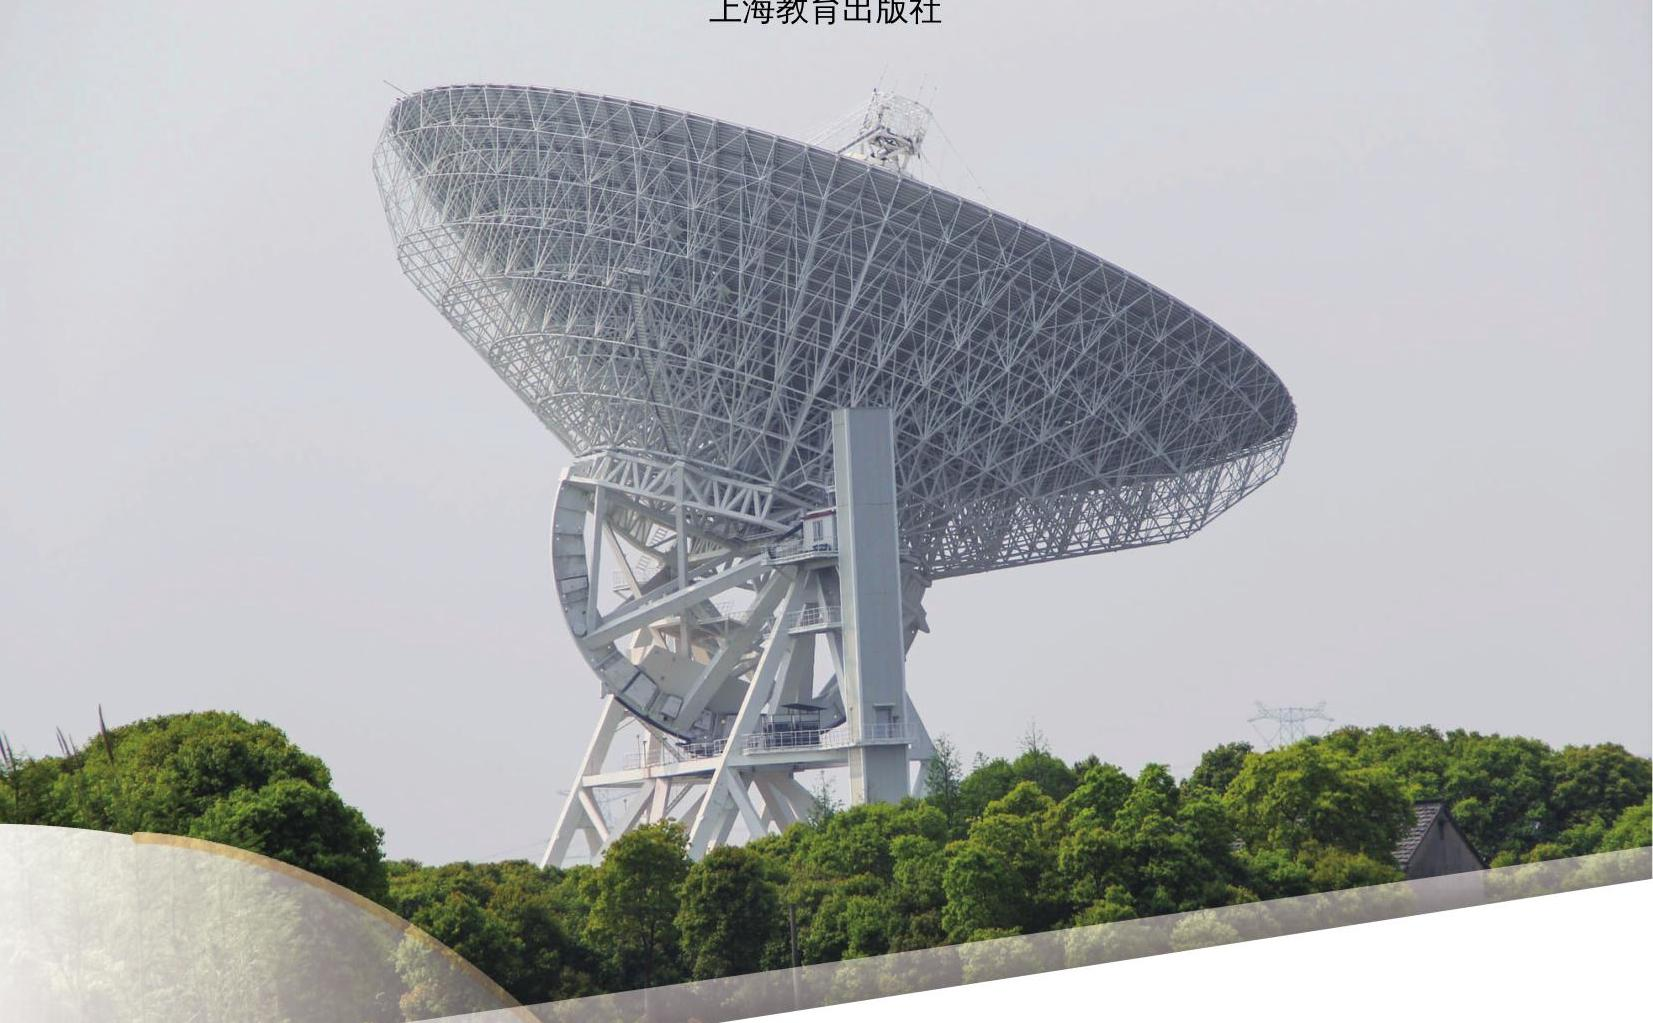
\includegraphics[max width=1.0\textwidth]{images/bo_d7fr3gc91nqc7381iccg_69_1_35_1653_1023_0.jpg}
\end{center}
\hspace*{3em} 

关于幂我们并不陌生, 在初中时已经学过正整数指数幂及其基本的运算性质, 并经历了将正整数指数幂推广到整数指数幂的过程. 本章通过定义分数指数幂, 将指数从整数拓展到有理数, 再引入无理数指数幂, 最终将指数从有理数拓展到实数. 这为下一章用幂函数描述变量之间的相应关系作好准备.

本章还将学习对数这一个新的概念, 它是指数运算的逆运算. 16 世纪末，随着当时天文、航海及工程实践的迅速发展，大量多位数乘除及开方的计算困扰着那时的科学家和工程师. 在简化计算的迫切需求下, 对数这个概念得以诞生, 并在实际计算中得到广泛应用. 现在，功能强大的现代计算器使多位数的乘除及开方计算变得非常方便, 对数用于简化计算的功能已经完成了其历史任务. 但是, 对数这个概念及对数函数的种种性质在现代数学和其他科学领域中的作用却有增无减，一直占据着重要的位置.

\section*{}

\section*{3.1 幂与指数}

\section*{1 指数幂的拓展}

在初中我们已经学过正整数指数幂的定义和运算性质.

Q

如果 \(a\) 是一个实数, \(n\) 是一个正整数,那么称

\[
{a}^{n} = \underset{n\text{ 个 }a}{\underbrace{a \cdot  a \cdot  \cdots  \cdot  a}}
\]

为 \(a\) 的 \(n\) 次幂. 正整数指数幂满足如下的运算性质:

Q 对任意给定的实数 \(a\text{ 、 }b\) 及正整数 \(s\text{ 、 }t\) ,有

(1) \({a}^{s}{a}^{t} = {a}^{s + t}\) ；

(2) \({\left( {a}^{s}\right) }^{t} = {a}^{st}\) ；

(3) \({\left( ab\right) }^{t} = {a}^{t}{b}^{t}\) .

为了定义整数指数幂, 我们在保证上述幂的运算性质仍然成立的条件下定义 \({a}^{0}\) 及 \({a}^{-n}\) ( \(n\) 为正整数).

假设性质 (1) 对所有的整数 \(s\text{ 、 }t\) 均成立,则当 \(s = 1,t = 0\) 时, 有

\[
a = {a}^{1 + 0} = {a}^{1} \cdot  {a}^{0} = a \cdot  {a}^{0}.
\]

所以,当 \(a \neq  0\) 时, \({a}^{0} = 1\) .

当 \(s = n,t =  - n\) 时,有

\[
{a}^{n + \left( {-n}\right) } = {a}^{n} \cdot  {a}^{-n} = {a}^{0} = 1.
\]

所以,当 \(a \neq  0\) 时, \({a}^{-n} = \frac{1}{{a}^{n}}\) .

因此,当 \(a \neq  0\) 时,可以定义

Q

\[
\left\{  \begin{array}{l} {a}^{0} = 1, \\  {a}^{-n} = \frac{1}{{a}^{n}}. \end{array}\right.
\]

这样,可以证明对任意给定的非零实数 \(a\text{ 、 }b\) 及整数 \(s\text{ 、 }t\) ,上述幂的运算性质 (1) 至 (3) 仍然成立.

在定义了整数指数幂后, 就会问: 能否定义有理数指数幂

\section*{}

\HRule

\(a\) 的 \(n\) 次方叫做 \(a\) 的 \(n\) 次幂,记作 \({a}^{n}\) . 称 \(a\) 为幂的底数(简称为底), \(n\) 为幂的指数.

同底数的幂相乘, 底数不变, 指数相加.

\[
{a}^{0} = 1\left( {a \neq  0}\right) .
\]

\HRule

呢? 答案是肯定的. 为此先拓展根式的概念.

一般地,如果 \(n\) 为大于 1 的整数,且 \({x}^{n} = a\) ,那么 \(x\) 叫做 \(a\) 的 \(n\) 次方根.

当 \(n\) 是奇数时,正数的 \(n\) 次方是一个正数,负数的 \(n\) 次方是一个负数, \(a\) 的 \(n\) 次方根是唯一存在的,且可用 \(\sqrt[n]{a}\) 表示. 例如,因为 \({2}^{5} = {32}\) ,所以 \(\sqrt[5]{32} = 2\) ; 因为 \({\left( -2\right) }^{5} =  - {32}\) ,所以 \(\sqrt[5]{-{32}} =  - 2.\)

但当 \(n\) 是偶数时,互为相反数的两个数的 \(n\) 次方是同一个数,一个正数的 \(n\) 次方根有两个,它们互为相反数. 这时,正数 \(a\) 的正的 \(n\) 次方根用 \(\sqrt[n]{a}\) 表示,而负的 \(n\) 次方根用 \(- \sqrt[n]{a}\) 表示,它们可以合并简写成 \(\pm  \sqrt[n]{a}\left( {a > 0}\right)\) . 例如,16 的 4 次方根可以表示为 \(\sqrt[4]{16} = 2\) 及 \(- \sqrt[4]{16} =  - 2\) ,简记为 \(\pm  \sqrt[4]{16} =  \pm  2\) . 显然,负数没有偶数次方根.

0 的任何次方根都是 0,记作 \(\sqrt[n]{0} = 0\) .

式子 \(\sqrt[n]{a}\) 叫做 \(a\) 的 \(n\) 次根式,这里 \(n\) 叫做根指数, \(a\) 叫做被开方数.

例 1 ( 1 )求 \(- \frac{1}{32}\) 的 5 次方根；

( 2 )求 81 的 4 次方根.

解( 1 )因为 \({\left( -\frac{1}{2}\right) }^{5} =  - \frac{1}{32}\) ，所以 \(\sqrt[5]{-\frac{1}{32}} =  - \frac{1}{2}\) .

(2)因为 \({\left( \pm 3\right) }^{4} = {81}\) ，所以 \(\pm  \sqrt[4]{81} =  \pm  3\) .

例 2 求下列各根式的值:

(1) \(\sqrt[5]{{\left( -2\right) }^{5}}\) ；

(2) \(\sqrt[6]{{\left( -8\right) }^{2}}\) .

\HRule

当 \(n\) 为奇数时, \(\sqrt[n]{{a}^{n}} = a\)

当 \(n\) 为偶数时, \(\sqrt[n]{{a}^{n}} = \left| a\right| .\)

\HRule

解 (1) \(\sqrt[5]{{\left( -2\right) }^{5}} =  - 2\) .

(2) \(\sqrt[6]{{\left( -8\right) }^{2}} = \sqrt[6]{{8}^{2}} = \sqrt[6]{{2}^{6}} = 2\) .

\section*{练习 3.1(1)}

1. 求 \(- \frac{32}{243}\) 的 5 次方根.

2. 求 9 的 4 次方根.

3. 求下列各根式的值:

(1) \(\sqrt[5]{{\left( -4\right) }^{5}}\) ； (2) \(\sqrt[6]{{\left( a - b\right) }^{6}}\) (其中 \(a < b\) ).

为了定义有理数指数幂, 我们首先定义正数的有理数指数幂, 使得整数指数幂的三条运算性质对有理数指数幂仍然成立.

设 \(a > 0,s\) 为有理数,我们定义 \({a}^{s}\) .

当 \(s = \frac{1}{n}\) ,而 \(n\) 是正整数时,若 \(n = 1\) ,则 \({a}^{\frac{1}{n}} = a\) ,这种情况比较特殊,无需定义; 若 \(n\) 大于 1,则定义 \({a}^{\frac{1}{n}} = \sqrt[n]{a}\) ,即为 \(a\) 的 \(n\) 次根式,它是方程 \({x}^{n} = a\) 的唯一正数解.

Q

\HRule

\({a}^{\frac{1}{n}} = \sqrt[n]{a}(a > 0,n\) 为大于 1 的整数).

\HRule

当 \(s = \frac{m}{n}\) ,而 \(m\) 是一个整数, \(n\) 是一个大于 1 的整数时, 定义

9

\[
{a}^{\frac{m}{n}} = {\left( {a}^{m}\right) }^{\frac{1}{n}} = \sqrt[n]{{a}^{m}}.
\]

\HRule

当 \(a < 0\) 且 \(n\) 是正奇数时, 存在唯一的实数 \(x\) ,使得

\({x}^{n} = a < 0,\) 此时 \({a}^{\frac{1}{n}}\) 能被定义.

当 \(a < 0\) 且 \(n\) 是正偶数时, 因为不存在实数 \(x\) ,使得

\({x}^{n} = a < 0,\)

故不能定义 \({a}^{\frac{1}{n}}\) .

当 \(a = 0\) 且 \(n\) 是正整数时, 也可定义 \({0}^{\frac{1}{n}} = 0\) .

\HRule

可以证明,当 \(\frac{m}{n} = \frac{{m}^{\prime }}{{n}^{\prime }}\) 且 \({m}^{\prime }\) 为整数及 \({n}^{\prime }\) 为大于 1 的整数时,总成 \(\dot{\text{ 工 }}{a}^{\frac{m}{n}} = {a}^{\frac{{m}^{\prime }}{{n}^{\prime }}}.\)

当 \(s\) 为有理数时,它总可表示为两个互素整数的商 \(\frac{m}{n}\) ,其中 \(m\) 是整数,而 \(n\) 是正整数,可定义 \({a}^{s} = {a}^{\frac{m}{n}}\) .

根据 \(\frac{1}{n}\) 次幂的定义,有 \({\left( {a}^{\frac{1}{n}}\right) }^{n} = a\) . 再由分数指数幂的定义与整数指数幂的运算性质 (2), 有

Q

\[
{\left( {a}^{\frac{1}{n}}\right) }^{m} = {\left( {a}^{\frac{1}{n}}\right) }^{\frac{nm}{n}} = {\left\lbrack  {\left( {a}^{\frac{1}{n}}\right) }^{nm}\right\rbrack  }^{\frac{1}{n}} = {\left\lbrack  {\left( {\left( {a}^{\frac{1}{n}}\right) }^{n}\right) }^{m}\right\rbrack  }^{\frac{1}{n}} = {\left( {a}^{m}\right) }^{\frac{1}{n}}.
\]

\HRule

一般地,在 \(n\) 为大于 1 的整数,且 \(m\) 为整数时,对所有使得 \(\sqrt[n]{{a}^{m}}\) 有意义的实数 \(a\) ,都可定义

\({a}^{\frac{m}{n}} = \sqrt[n]{{a}^{m}}.\)

\HRule

因此,也可以把 \({a}^{\frac{m}{n}}\) 等价地定义为

\[
{a}^{\frac{m}{n}} = {\left( {a}^{\frac{1}{n}}\right) }^{m} = {\left( \sqrt[n]{a}\right) }^{m}.
\]

利用整数指数幂的运算性质(1)至(3)，可以证明这三条性质对有理数指数幂仍然成立. 我们也可以证明以下的幂的基本不等式: 当实数 \(a > 1\) ,有理数 \(s > 0\) 时,不等式 \({a}^{s} > 1\) 成立.

例 3 求下列各式的值:

(1) \({4}^{\frac{3}{2}}\) ；

(2) \({\left( \frac{81}{625}\right) }^{-\frac{3}{4}}\) .

解 反复利用有理数指数幂的运算性质, 可得

(1) \({4}^{\frac{3}{2}} = {\left( {2}^{2}\right) }^{\frac{3}{2}} = {2}^{3} = 8\) .

\section*{}



(2) \({\left( \frac{81}{625}\right) }^{-\frac{3}{4}} = {\left( \frac{625}{81}\right) }^{\frac{3}{4}} = {\left\lbrack  {\left( \frac{625}{81}\right) }^{\frac{1}{4}}\right\rbrack  }^{3} = {\left( \frac{5}{3}\right) }^{3} = \frac{125}{27}\) .

例 4 用有理数指数幂的形式表示下列各式(其中 \(a > 0\) ):

(1) \(\sqrt[3]{{a}^{2}}\) ；

(2) \({a}^{3} \cdot  \sqrt[4]{{a}^{3}}\) ；

(3) \(\sqrt{a\sqrt{a}}\) .

解 由有理数指数幂的定义和运算性质, 可得

(1) \(\sqrt[3]{{a}^{2}} = {a}^{\frac{2}{3}}\) .

(2) \({a}^{3} \cdot  \sqrt[4]{{a}^{3}} = {a}^{3} \cdot  {a}^{\frac{3}{4}} = {a}^{3 + \frac{3}{4}} = {a}^{\frac{15}{4}}\) .

(3) \(\sqrt{a\sqrt{a}} = {\left( a \cdot  {a}^{\frac{1}{2}}\right) }^{\frac{1}{2}} = {\left( {a}^{\frac{3}{2}}\right) }^{\frac{1}{2}} = {a}^{\frac{3}{4}}\) .

下面我们考虑正数的无理数指数幂，在上述对正数的有理数指数幂定义的基础上，可以证明:对任意一个正数 \(a\) 与任意一个无理数 \(s\) ,可确定一个唯一的实数,记作 \({a}^{s}\) ,使得上述有理数指数幂的三条运算性质与幂的基本不等式对所有的实数 \({a}^{s}\) 都成立. 我们把这个实数 \({a}^{s}\) 定义为 \(a\) 的 \(s\) 次幂.

这样,当指数幂从正整数拓展到实数时,我们要求底 \(a\) 是一个正数. 此时指数幂满足以下的运算性质与幂的基本不等式.

性质 对任意给定的正数 \(a\text{ 、 }b\) 及实数 \(s\text{ 、 }t\) ,有

\[
{a}^{s}{a}^{t} = {a}^{s + t},
\]

\[
{\left( {a}^{s}\right) }^{t} = {a}^{st},
\]

\[
{\left( ab\right) }^{t} = {a}^{t}{b}^{t}.
\]

定理 当 \(a > 1,s > 0\) 时, \({a}^{s} > 1\) .

例 5 化简下列各式:

(1) \({\left( {x}^{\frac{\sqrt{3}}{2}}\right) }^{\sqrt{3}} \cdot  \sqrt{x}\) (其中 \(x > 0\) )；

(2) \(\frac{\left( {{a}^{\frac{2}{3}}{b}^{\frac{1}{2}}}\right) \left( {-3{a}^{\frac{1}{2}}{b}^{\frac{1}{3}}}\right) }{\frac{1}{3}{a}^{\frac{1}{6}}{b}^{\frac{5}{6}}}\) (其中 \(a > 0,b > 0\) ).

解(1)反复应用上述运算性质，可得



\HRule

这个证明要用到无理数由有理数逼近的性质, 相当繁复, 此处略去不讲.

此定理常称为幂的基本不等式, 在后面学习中还会用到.

\HRule

\section*{}

\[
{\left( {x}^{\frac{3}{2}}\right) }^{\sqrt{3}} \cdot  \sqrt{x} = {x}^{\frac{3}{2} \times  \sqrt{3}} \cdot  {x}^{\frac{1}{2}} = {x}^{\frac{3}{2}} \cdot  {x}^{\frac{1}{2}} = {x}^{\frac{3}{2} + \frac{1}{2}} = {x}^{2}.
\]

(2)由有理数指数幂的运算性质, 可得

\[
\frac{\left( {{a}^{\frac{2}{3}}{b}^{\frac{1}{2}}}\right) \left( {-3{a}^{\frac{1}{2}}{b}^{\frac{1}{3}}}\right) }{\frac{1}{3}{a}^{\frac{1}{6}}{b}^{\frac{5}{6}}} = \left( {-3 \times  3}\right) {a}^{\frac{2}{3} + \frac{1}{2} - \frac{1}{6}}{b}^{\frac{1}{2} + \frac{1}{3} - \frac{5}{6}} =  - {9a}{b}^{0} =  - {9a}.
\]

\section*{练习 3.1(2)}

1. 求下列各式的值:

(1) \({100}^{\frac{1}{2}}\) ;

(2) \({8}^{-\frac{2}{3}}\) .

2. 用有理数指数幂的形式表示下列各式(其中 \(a > 0\) ):

(1) \({a}^{\frac{10}{3}} \cdot  \sqrt[5]{{a}^{3}}\) ；

(2) \(\sqrt[3]{a\sqrt[3]{a}}\) .

3. 化简下列各式:

(1) \({\left( {a}^{3 + \sqrt{3}}\right) }^{3 - \sqrt{3}}\) (其中 \(a > 0\) )；

(2) \(\frac{4{a}^{\frac{2}{3}}{b}^{2}}{\left( {{a}^{\frac{1}{6}}{b}^{\frac{5}{6}}}\right) \left( {-\frac{2}{3}{a}^{\frac{1}{2}}b}\right) }\) (其中 \(a > 0,b > 0\) ).

4. 已知 \(0 < a < 1,s > 0\) . 求证: \(0 < {a}^{s} < 1\) .

\section*{习题 3.1}

A 组

1.(1)求-64的立方根； (2)求 256 的 4 次方根.

2. 求下列各根式的值:

(1) \(\sqrt[5]{\frac{243}{32}}\) ； (2) \(- \sqrt[3]{0.125}\) ；

(3) \(\sqrt[7]{{\left( -2\right) }^{7}}\) ； (4) \(\sqrt[6]{{\left( -{27}\right) }^{2}}\) .

3. 用有理数指数幂的形式表示下列各式(其中 \(x > 0,y > 0)\) :

(1) \(\sqrt[3]{{x}^{5}}\) ； (2) \({\left( \sqrt[5]{x}\right) }^{3}\) ；

(3) \(\sqrt[7]{{x}^{3}{y}^{4}}\)

(4) \(\sqrt{\frac{{x}^{3}}{{y}^{4}}}\) .



4. 用根式的形式表示下列各式(其中 \(a > 0\) ):

(1) \({a}^{\frac{2}{3}}\) ； (2) \({a}^{\frac{3}{4}}\) ；

(3) \({a}^{-\frac{2}{5}}\) ； (4) \({a}^{-\frac{5}{2}}\) .

5. 求下列各式中 \(x\) 的值(其中 \(x > 0\) ):

(1) \({x}^{3} = {27}\) ； (2) \({x}^{4} = {121}\) ；

(3) \({x}^{\frac{3}{2}} = {1000}\) ； (4) \({x}^{-\frac{4}{3}} = \frac{16}{625}\) .

6. 用有理数指数幂的形式表示下列各式(其中 \(a > 0,b > 0\) ):

(1) \({a}^{\frac{1}{3}}{a}^{\frac{1}{4}}\) ； (2) \(\sqrt[3]{a\sqrt{a}}\) ；

(3) \({\left( {a}^{\frac{1}{4}}{b}^{-\frac{3}{8}}\right) }^{8}\) ；

(4) \({\left( \frac{{a}^{-3}{b}^{4}}{\sqrt{b}}\right) }^{-\frac{1}{3}}\) .

7. 化简下列各式(其中 \(a > 0,b > 0\) ):

(1) \(\frac{\left( {2{a}^{\frac{2}{3}}{b}^{\frac{1}{2}}}\right) \left( {-6{a}^{\frac{1}{2}}{b}^{\frac{1}{3}}}\right) }{3{a}^{\frac{1}{6}}{b}^{\frac{5}{6}}}\) ;

(2) \({\left( {a}^{2 - \sqrt{3}}b\right) }^{2 + \sqrt{3}} \cdot  {b}^{2 - \sqrt{3}}\) .

B 组

1. 当 \(x < 0\) 时,求 \(\left| x\right|  + \sqrt[6]{{x}^{6}} + 2\sqrt[3]{{x}^{3}}\) 的值.

2. 设 \({a}^{2x} = 2\) ,且 \(a > 0\) . 求 \(\frac{{a}^{3x} + {a}^{-{3x}}}{{a}^{x} + {a}^{-x}}\) 的值.

3. 设 \(a > b > 0\) ,求证: \({a}^{a}{b}^{b} > {\left( ab\right) }^{\frac{a + b}{2}}\) .

\section*{3.2 对数}

\section*{1 对数的定义}

\begin{center}
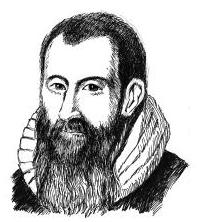
\includegraphics[max width=0.2\textwidth]{images/bo_d7fr3gc91nqc7381iccg_76_252_742_197_222_0.jpg}
\end{center}
\hspace*{3em} 

纳皮尔(J. Napier, 1550 - 1617)，苏格兰数学家，对数的发明者.

想象这样一个场景, 某人在银行存入 1 万元, 若年利率为 5\%，且按年计复利，经过多少年 1 万元存款才能连本带利超过 5 万元呢?

年利率为 5\% 的意思是一年之后 1 万元变成 \(1 \times  \left( {1 + 5\% }\right)  =\) 1.05 万元. 按年计复利的意思是每过一年自动将连本带利作为本金再次存入银行生息. 这样,经过 \(n\) 年后,存款连本带利的总数应达到 \({1.05}^{n}\) 万元. 根据题意,我们要回答,当 \(n\) 是多少时,

\[
{1.05}^{n} > 5\text{ ? }
\]

实际上,如果能够找到一个数 \(x\) ,使得 \({1.05}^{x} = 5\) ,那么 \(n\) 就是大于 \(x\) 的最小整数.

抽象一下上面的问题: 设 \(a > 0,N > 0\) ,要找 \(x\) ,使得

\[
{a}^{x} = N\text{ . }
\]
  \circled{1} 

要讨论这个问题,首先要假设 \(a > 0\) ,以保证对所有的 \(x\) , \({a}^{x}\) 都有定义. 还要假设 \(a \neq  1\) ,因为如果 \(a = 1,{a}^{x}\) 就恒等于 1, 在 \(N > 0\) 且 \(N \neq  1\) 时,方程 \circled{1} 无解; 而在 \(N = 1\) 时,方程 \circled{1} 有解但不唯一.

此外,在 \(a > 0\) ,且 \(a \neq  1\) 时,只要 \(N > 0\) ,方程 \({a}^{x} = N\) 总有唯一的解.

定义 在 \(a > 0,a \neq  1\) ,且 \(N > 0\) 的条件下,唯一满足 \({a}^{x} = N\) 的数 \(x\) ,称为 \(N\) 以 \(a\) 为底的对数 (logarithm),并用符号 \({\log }_{a}N\) 表示,而 \(N\) 称为真数.

\HRule

对数的底是不等于 1 的正数.

\HRule

Q

\HRule

"log" 是拉丁文 logarithmus 的缩写.

\HRule

这样, 在讨论对数的时候, 我们总是假设底是不等于 1 的正数,并且假设真数是正数. 另外,由定义,对数 \({\log }_{a}N\) 这个记号表示满足方程 \({a}^{x} = N\) 的唯一确定的数 \(x\) . 因此

\[
{a}^{{\log }_{a}N} = N.
\]
  \circled{2} 



这个式子看起来很玄妙, 但不过是对数定义的另一个表达方式而已, 也充分说明对数运算是指数运算的逆运算.

由此恒等式可以推出,若两个正数 \(M\text{ 、 }N\) 的对数 \({\log }_{a}M\) 与 \({\log }_{a}N\) 相等,则 \(M = N\) ,即若同一个底的两个对数相等,则其真数必相等. 这是因为

\[
M = {a}^{{\log }_{a}M} = {a}^{{\log }_{a}N} = N.
\]

此外,因为 \({a}^{0} = 1,{a}^{1} = a\) ,易见

\[
{\log }_{a}1 = 0,{\log }_{a}a = 1.
\]

在一些特殊情况下, 可以写出对数的具体数值, 而在一般情况下, 估算对数的精确值极为困难, 需要查阅有关的对数表或利用计算器来得到对数的近似值.

例 1 求下列各式的值:

(1)lo \({\text{ g }}_{2}8\) ；

(2)lo \({\text{ g }}_{2}\sqrt{2}\) ；

(3) \({\log }_{10}{0.000}\) 01.

解(1)因为 \({2}^{3} = 8\) ，即 3 是方程 \({2}^{x} = 8\) 的唯一解，所以由定义得 \({\log }_{2}8 = 3\) .

(2)因为 \({2}^{\frac{1}{2}} = \sqrt{2}\) ，所以 \({\log }_{2}\sqrt{2} = \frac{1}{2}\) .

(3)因为 \({10}^{-5} = {0.00001}\) ，所以 \({\log }_{10}{0.00001} =  - 5\) .

对数的底 \(a\left( {a > 0\text{ 且 }a \neq  1}\right)\) 原则上可以任意选取,数学上常用两个特殊的底构成的对数.

以 10 为底的对数称为常用对数 (common logarithm). \({\log }_{10}N\) 通常记为 \(\lg N\) . 在中学阶段,我们主要采用常用对数, 因为在日常生活中用的数字是十进制表示的.

以无理数 \(\mathrm{e}\) ( \(\mathrm{e}\) 的值约为 \({2.71828}\cdots\) ) 为底的对数称为自然对数 (natural logarithm). \({\log }_{\mathrm{e}}N\) 通常记为 \(\ln N\) . 虽然自然对数在日常生活中不常使用，但在高等数学和其他科学领域中却十分有用， 大家将来学到高等数学时，会很容易地看到这一点.

例 2 求下列各式中 \(x\) 的值:

(1)lo \({g}_{2}x =  - 1\) ;

(2) \({\log }_{\frac{1}{2}}x = 3\) ；

(3) \(\ln x =  - 1\) .

解 (1) 由 \({\log }_{2}x =  - 1\) ,得 \(x = {2}^{-1} = \frac{1}{2}\) .

(2)由 \({\log }_{\frac{1}{2}}x = 3\) ,得 \(x = {\left( \frac{1}{2}\right) }^{3} = \frac{1}{{2}^{3}} = \frac{1}{8}\) .

(3)由 \(\ln x =  - 1\) ，得 \(x = {\mathrm{e}}^{-1} = \frac{1}{\mathrm{e}}\) .

\section*{练习 3.2(1)}

1. 以下对数式中,与指数式 \({5}^{x} = 6\) 等价的是 ( )

A. \({\log }_{5}6 = x\) ; B. \({\log }_{5}x = 6\) ;

C. \({\log }_{6}x = 5\) ; D. \({\log }_{x}6 = 5\) .

2. 求下列各式的值:

(1) \({\log }_{5}{25}\) ; (2) \({\log }_{\frac{1}{3}}{27}\) ；

(3) \({\log }_{4}\sqrt{2}\) ； (4) \({2}^{{\log }_{2}3}\) .

3. 求下列各式中 \(x\) 的值:

(1) \({\log }_{4}x = 2\) ； (2) \({\log }_{x}4 = 2\) .

\section*{2 对数的运算性质}

引进对数的初衷是为了处理多位数的乘除及开方. 在本节中可以看到, 对数可以把乘除运算转变为加减运算, 并把乘方开方运算转化为乘除运算. 这为多位数的乘除及开方运算提供了一条简便的途径.

我们知道指数的运算性质: 对任意给定的正数 \(a\) 及实数 \(s\) 、 \(t\) ,有

\[
{a}^{s + t} = {a}^{s}{a}^{t},
\]

通俗地说, 指数可以把加减转化为乘除. 这个性质在对数中怎么体现呢?

在本节中,我们总假设 \(a > 0\) ,且 \(a \neq  1\) .

设 \(M > 0,N > 0\) ,令 \(b = {\log }_{a}M,c = {\log }_{a}N\) ,就有 \({a}^{b} = M\) , \({a}^{c} = N\) ,因此

\[
{MN} = {a}^{b}{a}^{c} = {a}^{b + c}.
\]

从而, 由对数的定义, 有

\[
{\log }_{a}\left( {MN}\right)  = b + c = {\log }_{a}M + {\log }_{a}N.
\]

\section*{}



由此可得下述对数运算的基本性质.

对数性质 1 当 \(M > 0,N > 0\) 时,

\[
{\log }_{a}\left( {MN}\right)  = {\log }_{a}M + {\log }_{a}N.
\]

由性质 1 可以推出

\[
{\log }_{a}M = {\log }_{a}\left( {\frac{M}{N} \cdot  N}\right)  = {\log }_{a}\frac{M}{N} + {\log }_{a}N,
\]

从而得到

对数性质 2 当 \(M > 0,N > 0\) 时,

\[
{\log }_{a}\frac{M}{N} = {\log }_{a}M - {\log }_{a}N.
\]

对数性质 1 与 2 可以通俗地解释为:对数把乘除运算转化为加减运算.

设 \(N > 0\) ,令 \(b = {\log }_{a}N\) ,则 \(N = {a}^{b}\) . 由 \({\left( {a}^{b}\right) }^{c} = {a}^{bc}\) ,得 \({a}^{bc} = {N}^{c}\) ,从而由对数的定义, \({bc} = {\log }_{a}{N}^{c}\) . 所以,我们有

对数性质 3 当 \(N > 0\) 时,对任何给定的实数 \(c\) ,

\[
{\log }_{a}{N}^{c} = c{\log }_{a}N.
\]

特别地,当 \(c\) 为大于 1 的正整数 \(n\) 时,乘方转化为乘; 当 \(c = \frac{1}{n}\) 时,开方转化为除. 这说明: 对数把乘方及开方分别转化为乘与除.

例 3 求下列各式的值:

(1)log \({}_{3}\left( {{9}^{4} \times  {3}^{2}}\right)\) ;

(2) \({\log }_{3}\sqrt[5]{9}\) ；

(3) \(2{\log }_{5}{10} + {\log }_{5}3 - {\log }_{5}{12}\) .

解 反复应用上述对数性质, 可得

(1) \({\log }_{3}\left( {{9}^{4} \times  {3}^{2}}\right)  = {\log }_{3}{9}^{4} + {\log }_{3}{3}^{2}\)

\(= 4{\log }_{3}9 + 2{\log }_{3}3 \; = 4{\log }_{3}{3}^{2} + 2\)

\[
= 4 \times  2{\log }_{3}3 + 2
\]

\[
= 4 \times  2 + 2
\]

\[
= {10}\text{ . }
\]

\HRule

对数化乘为加、 化除为减.

对数化乘方为乘、 化开方为除.

\HRule



(2) \({\log }_{3}\sqrt[5]{9} = {\log }_{3}{3}^{\frac{2}{5}} = \frac{2}{5}{\log }_{3}3 = \frac{2}{5}\) .

(3) \(2{\log }_{5}{10} + {\log }_{5}3 - {\log }_{5}{12}\)

\[
= {\log }_{5}\frac{{10}^{2} \times  3}{12}
\]

\[
= {\log }_{5}{25} = 2\text{ . }
\]

例 4 已知 \({\log }_{5}2 = a,{5}^{b} = 3\) ,用 \(a\) 及 \(b\) 表示 \({\log }_{5}{12}\) .

解 因为 \({5}^{b} = 3\) ,所以 \({\log }_{5}3 = b\) .

因此 \({\log }_{5}{12} = {\log }_{5}\left( {{2}^{2} \times  3}\right)  = 2{\log }_{5}2 + {\log }_{5}3 = {2a} + b\) .

例 5 在有声世界, 声强级是表示声强度相对大小的指标. 其值 \(y\) [单位: \(\mathrm{{dB}}\) (分贝)]定义为

\[
y = {10}\lg \frac{I}{{I}_{0}}.
\]

其中, \(I\) 为声场中某点的声强度,其单位为 \(\mathrm{W}/{\mathrm{m}}^{2}\) (瓦/平方米), \({I}_{0} = {10}^{-{12}}\mathrm{\;W}/{\mathrm{m}}^{2}\) 为基准值.

(1)如果 \(I = {10}\mathrm{\;W}/{\mathrm{m}}^{2}\) ，求相应的声强级；

(2)声强级为 60 dB 时的声强度 \({I}_{60}\) 是声强级为 50 dB 时的声强度 \({I}_{50}\) 的多少倍?

\HRule

\begin{center}
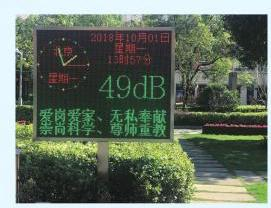
\includegraphics[max width=0.2\textwidth]{images/bo_d7fr3gc91nqc7381iccg_80_208_1241_271_208_0.jpg}
\end{center}
\hspace*{3em} 

一般地，正常交谈的声音是 \({60}\mathrm{{dB}}\) ，闹市区的声音是 \({80}\mathrm{\;{dB}}\) , 飞机起飞时的声音大约是 \({120}\mathrm{\;{dB}}\) .

\HRule

解(1)当 \(I = {10}\mathrm{W}/{\mathrm{m}}^{2}\) 时,

\[
y = {10}\lg \frac{I}{{I}_{0}} = {10}\lg \frac{10}{{10}^{-{12}}} = {10}\lg {10}^{13} = {130}\left( \mathrm{\;{dB}}\right) .
\]

因此,当 \(I = {10}\mathrm{\;W}/{\mathrm{m}}^{2}\) 时,相应的声强级为 \({130}\mathrm{\;{dB}}\) .

(2)由题意，得

\[
\left\{  \begin{array}{l} {60} = {10}\lg \frac{{I}_{60}}{{I}_{0}}, \\  {50} = {10}\lg \frac{{I}_{50}}{{I}_{0}}. \end{array}\right.
\]

两式相减, 得

\[
{10} = {10}\left( {\lg \frac{{I}_{60}}{{I}_{0}} - \lg \frac{{I}_{50}}{{I}_{0}}}\right)  = {10}\lg \frac{{I}_{60}}{{I}_{50}},
\]

即 \(\lg \frac{{I}_{60}}{{I}_{50}} = 1\) ,所以 \(\frac{{I}_{60}}{{I}_{50}} = {10}\) .

因此，声强级为 \({60}\mathrm{\;{dB}}\) 时的声强度 \({I}_{60}\) 是声强级为 \({50}\mathrm{\;{dB}}\) 时的声强度 \({I}_{50}\) 的 10 倍.



\section*{练习 3.2(2)}

1. 已知 \(A = {\log }_{a}x,B = {\log }_{a}y\left( {a > 0\text{ 且 }a \neq  1}\right)\) . 用 \(A\) 及 \(B\) 表示下列各式:

(1) \({\log }_{a}{xy}\) ；

(2) \({\log }_{a}\frac{{x}^{2}}{\sqrt{y}}\) .

2. 求下列各式的值:

(1) \({\log }_{15}3 + {\log }_{15}5\) (2) \({\log }_{2}\sqrt[3]{4}\) ；

(3) \({\log }_{5}\sqrt{10} - \frac{1}{2}{\log }_{5}{250}\) .

3. 已知 \({\log }_{7}3 = a,{7}^{b} = 2\) . 用 \(a\) 及 \(b\) 表示 \({\log }_{7}{72}\) .

\section*{3 对数的换底}

下面将介绍对数换底公式. 不同底的对数可以很方便地互相转换.

如前所述,对数的底 \(a\) 总是为不等于 1 的正数.

设 \(b > 0\) 且 \(b \neq  1\) 为另一个底,且 \(N > 0\) . 令 \(c = {\log }_{b}N\) ,即 \({b}^{c} = N\) . 由对数性质 3,得

\[
{\log }_{a}N = {\log }_{a}{b}^{c} = c{\log }_{a}b = {\log }_{b}N \cdot  {\log }_{a}b,
\]

因此得到

对数换底公式 当 \(N > 0\) 时,

\[
{\log }_{b}N = \frac{{\log }_{a}N}{{\log }_{a}b}.
\]

它把以 \(b\) 为底的对数换成两个以 \(a\) 为底的对数的商,其中 \({\log }_{a}b\) 只与两个底的值有关,而与真数 \(N\) 无关.

例如,估算 \({\log }_{2}3\) ,可先应用换底公式,得

\[
{\log }_{2}3 = \frac{\lg 3}{\lg 2}
\]

再利用计算器上的常用对数功能键,得 \(\lg 2 \approx  {0.3010},\lg 3 \approx  {0.4771}\) . 因此

\[
{\log }_{2}3 \approx  \frac{0.4771}{0.3010} \approx  {1.5850}.
\]





例 6 求下列各式的值:

(1) \({\log }_{2}{25} \times  {\log }_{3}4 \times  {\log }_{5}9\)

(2) \(\frac{1}{{\log }_{2}3} + \frac{\lg {13.5}}{\lg 3}\) .

解(1)把所有的对数换成同一个底，如都换成以 2 为底， 得到 Q

\[
{\log }_{2}{25} \times  {\log }_{3}4 \times  {\log }_{5}9 = {\log }_{2}{5}^{2} \times  {\log }_{3}{2}^{2} \times  {\log }_{5}{3}^{2}
\]

\[
= {\log }_{2}{5}^{2} \times  \frac{{\log }_{2}{2}^{2}}{{\log }_{2}3} \times  \frac{{\log }_{2}{3}^{2}}{{\log }_{2}5}
\]

\[
= 2{\log }_{2}5 \times  \frac{2{\log }_{2}2}{{\log }_{2}3} \times  \frac{2{\log }_{2}3}{{\log }_{2}5}
\]

\[
= 2 \times  2 \times  2 = 8\text{ . }
\]

\HRule

对数运算中, 用换底公式将不同的底换成同一个底是一种常用的方法.

\HRule

(2)将所有的对数统一换成常用对数，因 \({\log }_{2}3 = \frac{\lg 3}{\lg 2}\) ，有

\[
\frac{1}{{\log }_{2}3} + \frac{\lg {13.5}}{\lg 3} = \frac{\lg 2}{\lg 3} + \frac{\lg {13.5}}{\lg 3} = \frac{\lg {27}}{\lg 3} = \frac{\lg {3}^{3}}{\lg 3} = 3.
\]

例 7 设 \(a > 0,a \neq  1\) ,且 \(N > 0\) . 求证: 若 \(m \neq  0\) ,则 \({\log }_{{a}^{m}}{N}^{n} = \frac{n}{m}{\log }_{a}N.\)

证明 应用换底公式将底换成 \(a\) ,并利用 \({\log }_{a}a = 1\) ,得

\[
{\log }_{{a}^{m}}{N}^{n} = \frac{{\log }_{a}{N}^{n}}{{\log }_{a}{a}^{m}} = \frac{n{\log }_{a}N}{m}.
\]

\section*{练习 3.2(3)}

1. 求下列各式的值:

(1) \({\log }_{8}\frac{1}{4}\) ;

(2) \({\log }_{a}b \cdot  {\log }_{b}c \cdot  {\log }_{c}a\) ( \(a\) 、 \(b\) 、 \(c\) 均为不等于 1 的正数)；

(3) \({3}^{2 + {\log }_{9}4}\) ；

(4) \(\frac{{\log }_{5}2 \times  {\log }_{7}9}{{\log }_{5}\frac{1}{3} \times  {\log }_{7}2}\) .

2. 已知 \({\log }_{3}2 = a\) ,用 \(a\) 表示 \({\log }_{2}{96}\) .

3. 设 \(a\text{ 、 }b\) 是两个不等于 1 的正数,求证: \({\log }_{b}a = \frac{1}{{\log }_{a}b}\) .



\section*{习题 3.2}

\section*{A 组}

1. 把下列指数式写成对数式:

(1) \({3}^{4} = {81}\) ； (2) \({5}^{-\frac{1}{2}} = x\) .

2. 将下列对数式写成指数式:

(1) \({\log }_{\frac{1}{3}}{27} =  - 3\) ； (2) \({\log }_{2}\frac{1}{8} =  - 3\) .

3. 求下列各式的值:

(1) \({\log }_{3}{27}\) ; (2) \({\log }_{\frac{1}{2}}8\) ；

(3) \(\ln \frac{1}{\mathrm{e}} + \lg \sqrt{10}\) .

4. 求下列各式中 \(x\) 的值:

(1) \({\log }_{2}x = 5\) ；

(2) \({\log }_{\sqrt{5}}\frac{1}{125} = x\) ;

(3) \({\log }_{x}4 = \frac{1}{2}\) .

5. 求下列各式的值:

(1) \({\log }_{2}\left( {2 \times  \sqrt[3]{2}}\right)\) ； (2) \({\log }_{21}3 + {\log }_{21}7\)

(3) \({\log }_{5}\sqrt{6} - \frac{1}{2}{\log }_{5}{150}\) ； (4) \({3}^{{\log }_{3}1} + {\log }_{2}{48} - {\log }_{2}3\) ；

(5) \(3{\log }_{3}\frac{3}{2} - {\log }_{3}\frac{7}{4} + \frac{1}{2}{\log }_{3}4 + {\log }_{3}7\) .

6. 已知 \(A = {\log }_{a}x,B = {\log }_{a}y,C = {\log }_{a}z\left( {a > 0\text{ 且 }a \neq  1}\right)\) . 用 \(A\text{ 、 }B\) 及 \(C\) 表示下列各式:

(1) \({\log }_{a}\left( {x{y}^{2}}\right)\) ；

(2) \({\log }_{a}\frac{xy}{\sqrt{z}}\) ；

(3) \({\log }_{a}\left( {{x}^{2}{y}^{2}}\right)  + {\log }_{a}\left( {y\sqrt{x}}\right)\) .

7. 求下列各式的值:

(1) \({\log }_{4}2\sqrt{2}\) ； (2) \({\log }_{2}3 \times  {\log }_{9}2\) ；

(3) \(\frac{3}{{\log }_{2}6} + \frac{3}{{\log }_{3}6}\) ；

(4) \(\left( {{\log }_{4}3 + {\log }_{8}3}\right) \left( {{\log }_{3}2 + {\log }_{9}2}\right)  + {\log }_{\frac{1}{2}}\sqrt[4]{32}\) .

\section*{}

8. 已知 \(a = \lg 5\) ,用 \(a\) 表示 \(\lg 2\) 和 \(\lg {20}\) .

\section*{B 组}

1. 求下列各式中 \(x\) 的取值范围:

(1) \({\log }_{2}\left( {1 - {3x}}\right)\) ; (2) \({\log }_{a}\left( {{x}^{2} + x}\right) \left( {a > 0\text{ 且 }a \neq  1}\right)\) .

2. 求下列各式的值:

(1) \({\log }_{4}8 - {\log }_{\frac{1}{9}}3 - {\log }_{\sqrt{2}}4\) ； (2) \({2}^{{\log }_{6}5} \times  {3}^{{\log }_{6}5}\) ；

(3) \({\left( \lg {50}\right) }^{2} + \lg 2 \times  \lg {50}^{2} + {\left( \lg 2\right) }^{2}\) .

3. 科学家以里氏震级来度量地震的强度,若设 \(I\) 为地震时所散发出来的相对能量程度,则里氏震级度量 \(r\) 可定义为 \(r = \frac{2}{3}\lg I + 2\) . 求 7.8 级地震和 6.9 级地震的相对能量比值. (结果精确到个位)

4. 已知 \(\lg 2 = a,\lg 3 = b\) . 用 \(a\) 及 \(b\) 表示 \({\log }_{2}3\) 及 \({\log }_{12}{25}\) .

5. 已知 \({5.4}^{x} = 3,{0.6}^{y} = 3\) . 求 \(\frac{1}{x} - \frac{1}{y}\) 的值.

6. 设 \(a\text{ 、 }b\text{ 、 }c\text{ 、 }d\) 均为正数,且 \(a\text{ 、 }c\) 均不为 1 . 求证:

\[
{\log }_{a}b \cdot  {\log }_{c}d = {\log }_{a}d \cdot  {\log }_{c}b.
\]

\section*{课后阅读}

\section*{用对数简化计算}

让我们用一个例子说明怎样应用对数来简化计算.

假设我们要计算两个九位数的乘积

\[
{867432691} \times  {345723901}.
\]

直接计算费时费力，怎样利用对数来简化计算呢?

先求此乘积以 10 为底的对数

\[
\lg \left( {{867432691} \times  {345723901}}\right) \text{ . }
\]

由对数性质 1 , 它等于 \(\lg {867432691} + \lg {345723901}\) .

要直接计算这些对数自然十分困难, 但是如果已编制了一个常用对数表, 可以查真数在 1 到 10 之间的常用对数(实用中的对数表正是如此)，就可以得知

\[
\lg {867432691} \approx  \lg \left( {{8.6743} \times  {10}^{8}}\right)  = 8 + \lg {8.6743} \approx  {8.9382},
\]

其中 \(\lg {8.6743} \approx  {0.9382}\) 是查表得到的. 类似地,可得 \(\lg {345723901} \approx  {8.5387}\) . 这样所求乘积之对数为



\section*{}

\[
\lg {867432691} + \lg {345723901} \approx  {8.9382} + {8.5387} = {17.4769} = {17} + {0.4769}.
\]

为了最终求得所需要的乘积 867432691X345723901, 还需要查一个反对数表 (实际上是一个以 10 为底,而指数在 0 到 1 之间的指数表),就得到 \({0.4769} \approx  \lg {2.9985}\) ,即 \({10}^{0.4769} \approx  {2.9985}\) ,从而

\[
{17} + {0.4769} \approx  {17} + \lg {2.9985} = \lg \left( {{2.9985} \times  {10}^{17}}\right) ,
\]

即原乘积的常用对数约等于 \(\lg \left( {{2.9985} \times  {10}^{17}}\right)\) . 由于同底的两个对数相等,其真数必相等, 就得到

\[
{867432691} \times  {345723901} \approx  {2.9985} \times  {10}^{17}.
\]

(现在，用普通的计算器可以得到更精确的值

\[
{867432691} \times  {345723901} \approx  {2.998922138} \times  {10}^{17}\text{ ) }
\]

由上所述, 利用一个常用对数表及一个反对数表, 就可以通过转化为对数大大简化任何两个大数(多位数)的乘除及开方运算. 这正如恩格斯(F. Engles)所指出的: “这种从一个形态到另一个相反形态之转变, 并不是一种无聊的游戏, 它是数学科学最有力的模杆之一，如果没有它，今天就没法去进行一个较为复杂的计算. ”(《自然辩证法》)

然而, 制作一个有实际用处的对数表是一项浩大的工程, 假如按步长 0.001 从 1 变化到 10 , 就有 9 001 个对数要计算. 而要算一个数的对数使得精度达到四位小数, 也绝不是一件容易的事. 然而, 如果制成了对数表, 就可以一劳永逸地为其他人所用, 意义是十分重大的.

\section*{对数简史}

对数是纳皮尔发明的, 其出现事先似乎毫无征兆, 但它绝不是从天上掉下来的, 而是源自当时在天文、航海及工程实践中迫切需要简化大量繁杂计算的实际需要. 纳皮尔从 1594 年到 1614 年花了二十年的时间造出了第一个对数表, 他说过: “要实际应用数学, 我看最大的障碍就是处理很大数字的相乘、相除，或是求取二次或三次方根， \(\cdots \cdots\) 因此我开始思考，有没有什么方法可以去除这些障碍. ”由于对数不仅能将乘除运算化为加减运算, 而且能将乘方、开方运算化为乘除运算, 一下子将人们从繁复的计算中解放出来, 无异于成倍地延长了科学家与工程技术人员的寿命. 德国天文学家开普勒(J. Kepler)是最早使用对数的人之一, 他成功地在行星轨道的计算中运用了对数. 法国数学家、天文学家拉普拉斯 (P.-S. Laplace) 曾说过:“对数的发明让天文学家的寿命都延长了，因为少做了很多苦工. ”恩格斯曾经将解析几何、对数及微积分并列为最重要的数学方法.

在清代初年 (17 世纪中叶) 对数传到了中国, 1653 年薛凤柞与波兰人穆尼阁 (J. N. Smogolehshi)共同编译出版了《比例对数表》一书，正式将对数介绍到中国，薛凤柞还将对数应用到历法计算中. 后来, 康熙皇帝组织编撰《数理精蕴》一书, 在其下篇・卷三十八“对数比例”一节中，一开始就说:“对数比例乃西士若往·纳白尔(John Napier)所作，



幂、指数与对数以假数与真数对列成表，故名对数表. ”这个假数，我们现在叫“对数”，而若往・纳白尔就是我们现在所述的纳皮尔.

在科学发展的历史中，极少有哪个抽象的数学概念，能像对数一样，一开始就很快受到了整个科学界的热烈欢迎. 对数的发明, 无疑是人类认识史上一个极大的飞跃与革命, 在人类文明的进程中起了划时代的作用. 自纳皮尔 1614 年发明对数以来, 一直到袖珍计算器的出现, 对数以及根据对数的原理所设计的一些计算仪器, 一直是进行复杂计算的有效方法和工具. 根据对数原理设计的计算仪器, 最著名的就是后来为科学家和工程师广泛使用的计算尺, 它在长达 350 年的时间中, 一直是科学家与工程师的忠实伴侣和有力工具. 自 20 世纪 70 年代初期袖珍计算器上市以后, 计算尺才失去市场, 并随着计算机的飞速发展而彻底退出了历史舞台，对数在计算中无可替代的地位也一去而不复返了. 但是, 对数的概念及对数函数的种种性质在众多数学分支及科学领域中至今一直发挥着重要的作用, 并且有增无减. 对数从计算的有力工具向科学的重要方法的转化, 在数学的发展史上留下了浓墨重彩的篇章, 记录着人类不断走向文明进步的光辉历程.

\begin{center}
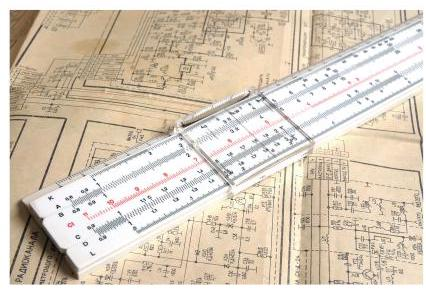
\includegraphics[max width=0.3\textwidth]{images/bo_d7fr3gc91nqc7381iccg_86_1072_739_426_291_0.jpg}
\end{center}
\hspace*{3em} 

\section*{内容提要}

1. 指数幂的拓展:正整数指数幂、整数指数幂、有理数指数幂、实数指数幂.

2. 幂的运算性质:对任意给定的正数 \(a\text{ 、 }b\) 及实数 \(s\text{ 、 }t\) ，

(1) \({a}^{s}{a}^{t} = {a}^{s + t}\) ；

(2) \({\left( {a}^{s}\right) }^{t} = {a}^{st}\) ；

(3) \({\left( ab\right) }^{t} = {a}^{t}{b}^{t}\) .

3. 对数的定义: 当 \(a\) 是不等于 1 的正数, \(N > 0\) 时, \(N \cup  a\) 为底的对数 \({\log }_{a}N\) 是满足

\[
{a}^{x} = N
\]

的唯一的数 \(x\) .

4. 对数的基本性质: 设 \(a\) 是不等于 1 的正数, \(M\) 及 \(N\) 是任意给定的正数, \(c\) 是任意给定的实数.

(1) \({\log }_{a}1 = 0\) ;

(2) \({\log }_{a}a = 1\) ;

(3) \({\log }_{a}\left( {MN}\right)  = {\log }_{a}M + {\log }_{a}N\) ；

(4) \({\log }_{a}\frac{M}{N} = {\log }_{a}M - {\log }_{a}N\) ;

(5) \({\log }_{a}{N}^{c} = c{\log }_{a}N\) ;

(6)(换底公式)如果 \(b\) 也是一个不等于 1 的正数，那么 \({\log }_{b}N = \frac{{\log }_{a}N}{{\log }_{a}b}\) .

\section*{复习题}

\section*{A 组}

1. 填空题:

(1)若 \({x}^{3} = 5\) ，则 \(x =\) \_\_\_\_\_；若 \({3}^{x} = 5\) ，则 \(x =\) \_\_\_\_\_.

(2)将 \(\sqrt[4]{a\sqrt[3]{a}}\left( {a > 0}\right)\) 化成有理数指数幂的形式为\_\_\_\_\_.

(3)若 \({\log }_{8}x =  - \frac{2}{3}\) ，则 \(x =\) \_\_\_\_\_.

(4)若 \({\log }_{a}b \cdot  {\log }_{5}a = 3\left( {a > 0\text{ 且 }a \neq  1}\right)\) ，则 \(b =\) \_\_\_\_\_.

\section*{}



幂、指数与对数

2. 选择题:

(1)若 \(\lg a\) 与 \(\lg b\) 互为相反数，则有 ( )

A. \(a + b = 0\) ; B. \({ab} = 1\) ;

C. \(\frac{a}{b} = 1\) ; D. 以上答案均不对.

(2)设 \(a > 0\) ，下列计算中正确的是 ( )

A. \({a}^{\frac{2}{3}} \cdot  {a}^{\frac{3}{2}} = a\) ; B. \({a}^{\frac{2}{3}} \div  {a}^{\frac{3}{2}} = a\) ;

C. \({a}^{-4} \cdot  {a}^{4} = 0\) ; D. \({\left( {a}^{\frac{2}{3}}\right) }^{\frac{3}{2}} = a\) .

3. 已知 \({10}^{\alpha } = 3,{10}^{\beta } = 4\) . 求 \({10}^{\alpha  + \beta }\) 及 \({10}^{\alpha  - \frac{\beta }{2}}\) 的值.

4. 求下列各式的值:

(1) \(\frac{1}{{4}^{x} + 1} + \frac{1}{{4}^{-x} + 1}\) ； (2) \({4}^{\sqrt{2} + 1} \times  {2}^{3 - 2\sqrt{2}} \times  {8}^{-\frac{2}{3}}\) .

5. 已知 \(\lg a < 1\) ,化简 \(\sqrt{{\left( \lg a\right) }^{2} - \lg \frac{{a}^{2}}{10}}\) .

6. 已知 \(m = {\log }_{2}{10}\) ,求 \({2}^{m} - m\lg 2 - 4\) 的值.

B 组

1. 填空题:

(1)若 \({4}^{x} = {2}^{-\frac{1}{2}},{4}^{y} = \sqrt[3]{32}\) ，则 \({2x} - {3y} =\) \_\_\_\_\_.

(2)若 \({\log }_{3}\left( {{\log }_{4}x}\right)  = 1\) ，则 \(x =\) \_\_\_\_\_.

(3)若 \({3}^{a} = {7}^{b} = {63}\) ，则 \(\frac{2}{a} + \frac{1}{b}\) 的值为\_\_\_\_\_.

2. 已知 \({\log }_{18}9 = a,{18}^{b} = 5\) ,则 \({\log }_{36}{45}\) 等于 ( )

A. \(\frac{a + b}{2 + a}\) ; B. \(\frac{a + b}{2 - a}\) ; C. \(\frac{a + b}{2a}\) ; D. \(\frac{a + b}{{a}^{2}}\) .

3. 设 \({\log }_{0.2}a > 0,{\log }_{0.2}b > 0\) ,且 \({\log }_{0.2}a \cdot  {\log }_{0.2}b = 1\) . 求 \({\log }_{0.2}\left( {ab}\right)\) 的最小值.

4. 化简 \(\frac{\left( {1 + {2}^{x}}\right) \left( {1 + {2}^{2x}}\right) \left( {1 + {2}^{4x}}\right) \left( {1 + {2}^{8x}}\right) \left( {1 + {2}^{16x}}\right) }{1 - {2}^{32x}}\) (其中 \(x \neq  0\) ).

5. 已知 \(a > 1,b > 0\) . 求证: 对任意给定的实数 \(k,{a}^{{2b} + k} - {a}^{b + k} > {a}^{b + k} - {a}^{k}\) .

\section*{拓展与思考}

1. 甲、乙两人同时解关于 \(x\) 的方程: \({\log }_{2}x + b + c{\log }_{x}2 = 0\) . 甲写错了常数 \(b\) ,得两根 \(\frac{1}{4}\) 及 \(\frac{1}{8}\) ; 乙写错了常数 \(c\) ,得两根 \(\frac{1}{2}\) 及 64 . 求这个方程的真正根.

2. 已知 \(a\text{ 、 }b\) 及 \(c\) 是不为 1 的正数,且 \(\lg a + \lg b + \lg c = 0\) . 求证:

\[
{a}^{\frac{1}{\lg b} + \frac{1}{\lg c}} \cdot  {b}^{\frac{1}{\lg c} + \frac{1}{\lg a}} \cdot  {c}^{\frac{1}{\lg a} + \frac{1}{\lg b}} = \frac{1}{1000}.
\]





第 4 章幂函数、指数函数与对数函数

初中已经学过一些基本的初等函数, 如正比例函数、 反比例函数、一次函数、二次函数等. 函数是描述客观世界中变量之间相互关系和变化规律的重要语言和工具. 例如, 一次函数可描述匀速运动，二次函数可描述匀加速运动等.

本章我们将在上一章的基础上,通过固定等式 \({a}^{b} = c\) 中的三个量 \(a\) 、 \(b\) 、 \(c\) 中的一个量,研究另两个量的相互关系和变化规律，定义三种基本而应用广泛的函数——幂函数、 指数函数和对数函数. 要学会用函数图像和代数运算的方法研究这些函数的性质, 了解它们各自蕴含的规律. 同时, 要通过建立数学模型, 解决一些简单的实际问题, 并体会这些函数在解决有关实际问题中的作用. 这些都将为下一章 “函数的概念、性质及应用”的学习奠定基础.

\section*{4.1 幂函数}

\section*{1 幂函数的定义与图像}

在初中阶段我们已经学过正比例函数如 \(y = x\) ,反比例函数如 \(y = \frac{1}{x}\) 即 \(y = {x}^{-1}\) ,以及二次函数如 \(y = {x}^{2}\) 等函数的图像与性质.

这三个函数的共同特征都是将幂的指数 \(a\) 固定,底数取为变量 \(x\) ,而研究幂 \({x}^{a}\) 随 \(x\) 的变化而变化的规律. 用

\[
y = {x}^{a}
\]

来描述 \(y\) 与 \(x\) 之间的关系就得到了幂函数.

定义 当指数 \(a\) 固定,等式

\[
y = {x}^{a}
\]

确定了变量 \(y\) 随变量 \(x\) 变化的规律,称为指数为 \(a\) 的幂函数 (power function).

使得 \({x}^{a}\) 有意义的 \(x\) 的取值范围,称为此幂函数的定义域. 幂函数的定义域可以是不相同的,它与指数 \(a\) 的值有关.

例 1 求下列函数的定义域:

(1) \(y = {x}^{3}\) ；

(2) \(y = {x}^{\frac{1}{2}}\) ；

(3) \(y = {x}^{-\frac{2}{3}}\) .

解(1)对一切实数 \(x\) 该函数都有意义,所以其定义域是 \(\mathbf{R}\) .

(2) \(y = {x}^{\frac{1}{2}} = \sqrt{x}\) ，当 \(x \geq  0\) 时，该函数才有意义，所以其定义域是 \(\lbrack 0, + \infty )\) .

(3) \(y = {x}^{-\frac{2}{3}} = \frac{1}{\sqrt[3]{{x}^{2}}}\) ，当 \(x \neq  0\) 时，该函数才有意义，所以其定义域是 \(\left( {-\infty ,0}\right)  \cup  \left( {0, + \infty }\right)\) .

\section*{}

\HRule

幂函数的指数 \(a \in  \mathbf{R}\) .

\HRule



函数图像是直观理解变量间关系的一个重要手段. 下面我们考察幂函数 \(y = {x}^{a}\) 的图像及性质.

在平面直角坐标系中把满足 \(y = {x}^{a}\) 的一切点 \(\left( {x,y}\right)\) 描绘出来,就构成幂函数 \(y = {x}^{a}\) 的图像. 需要注意,幂函数的图像依赖于指数 \(a\) 的值,可以有不同的形状.

\HRule

作出函数的大致图像的步骤可以是: 列表一描点一连线.

\HRule

\begin{center}
\adjustbox{max width=\textwidth}{
\begin{tabular}{|c|c|}
\hline
\(x\) & \(y = {x}^{\frac{1}{2}}\) \\
\cline{1-2}
0 & 0 \\
\cline{1-2}
0.25 & 0.5 \\
\cline{1-2}
0.5 & 0.7071 \\
\cline{1-2}
1 & 1 \\
\cline{1-2}
2 & 1.4142 \\
\cline{1-2}
4 & 2 \\
\cline{1-2}
6 & 2.4495 \\
\cline{1-2}
9 & 3 \\
\cline{1-2}
\hline
\end{tabular}
}
\end{center}

例 2 分别作出幂函数 \(y = {x}^{\frac{1}{2}}\) 及 \(y = {x}^{3}\) 的大致图像.

解 幂函数 \(y = {x}^{\frac{1}{2}}\) 的定义域为所有的非负数,我们在其图像上取一些特殊的点. 由

\[
{0}^{\frac{1}{2}} = 0,{\left( \frac{1}{4}\right) }^{\frac{1}{2}} = \frac{1}{2},{1}^{\frac{1}{2}} = 1,{4}^{\frac{1}{2}} = 2,{9}^{\frac{1}{2}} = 3,
\]

就得到幂函数 \(y = {x}^{\frac{1}{2}}\) 的图像过下面的点:

\[
\left( {0,0}\right) \text{ 、 }\left( {\frac{1}{4},\frac{1}{2}}\right) \text{ 、 }\left( {1,1}\right) \text{ 、 }\left( {4,2}\right) \text{ 、 }\left( {9,3}\right) .
\]

再使用计算器多采集一些点, 可以粗略地作出其图像, 如图 4-1-1(1)所示.

幂函数 \(y = {x}^{3}\) 的定义域为所有实数. 由

\[
{\left( -3\right) }^{3} =  - {27},{\left( -2\right) }^{3} =  - 8,{\left( -1\right) }^{3} =  - 1,{\left( -\frac{1}{2}\right) }^{3} =  - \frac{1}{8},
\]

\[
{0}^{3} = 0,{\left( \frac{1}{2}\right) }^{3} = \frac{1}{8},{1}^{3} = 1,{2}^{3} = 8,{3}^{3} = {27},
\]

就得到幂函数 \(y = {x}^{3}\) 的图像过下面的点:

\[
\left( {-3, - {27}}\right) \text{ 、 }\left( {-2, - 8}\right) \text{ 、 }\left( {-1, - 1}\right) \text{ 、 }\left( {-\frac{1}{2}, - \frac{1}{8}}\right) \text{ 、 }
\]

\[
\left( {0,0}\right) \text{ 、 }\left( {\frac{1}{2},\frac{1}{8}}\right) \text{ 、 }\left( {1,1}\right) \text{ 、 }\left( {2,8}\right) \text{ 、 }\left( {3,{27}}\right) \text{ . }
\]

再使用计算器多采集一些点, 可以粗略地作出其图像, 如图 4-1-1(2)所示.

\begin{center}
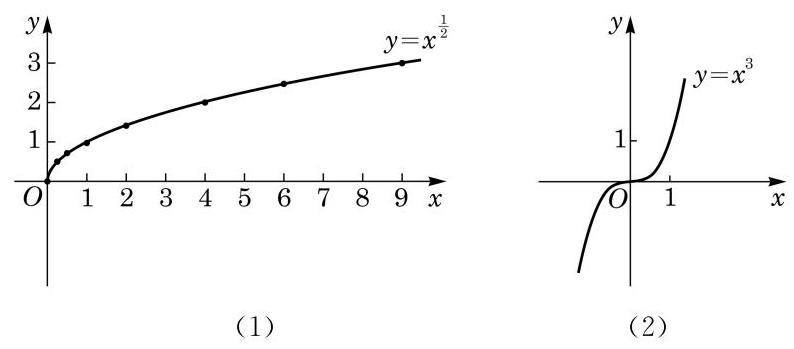
\includegraphics[max width=0.6\textwidth]{images/bo_d7fr3gc91nqc7381iccg_91_227_1706_794_349_0.jpg}
\end{center}
\hspace*{3em} 

图 4-1-1



\begin{center}
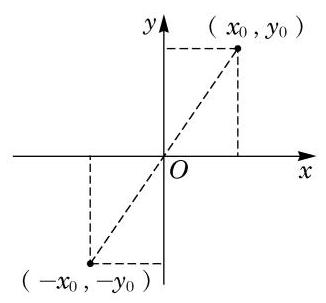
\includegraphics[max width=0.2\textwidth]{images/bo_d7fr3gc91nqc7381iccg_92_186_228_326_303_0.jpg}
\end{center}
\hspace*{3em} 

图 4-1-2

因为幂函数 \(y = {x}^{3}\) 的定义域为一切实数,若点 \(\left( {{x}_{0},{y}_{0}}\right)\) 在幂函数 \(y = {x}^{3}\) 的图像上,就有 \({y}_{0} = {x}_{0}^{3}\) . 而点 \(\left( {{x}_{0},{y}_{0}}\right)\) 关于原点的对称点易知是 \(\left( {-{x}_{0}, - {y}_{0}}\right)\) ,如图 4-1-2 所示. 由 \({y}_{0} = {x}_{0}^{3}\) ,得 \(- {y}_{0} = \; {\left( -{x}_{0}\right) }^{3}\) ,因此点 \(\left( {-{x}_{0}, - {y}_{0}}\right)\) 也落在幂函数 \(y = {x}^{3}\) 的图像上. 这说明幂函数 \(y = {x}^{3}\) 的图像关于原点成中心对称.

例 3 作出幂函数 \(y = {x}^{-\frac{2}{3}}\) 的大致图像.

解 因为 \({\left( -1\right) }^{-\frac{2}{3}} = \sqrt[3]{{\left( -\frac{1}{1}\right) }^{2}} = 1,{\left( -\frac{\sqrt{2}}{4}\right) }^{-\frac{2}{3}} = \sqrt[3]{{\left( -\frac{4}{\sqrt{2}}\right) }^{2}} \; = \sqrt[3]{8} = 2,{\left( \frac{\sqrt{2}}{4}\right) }^{-\frac{2}{3}} = \sqrt[3]{{\left( \frac{4}{\sqrt{2}}\right) }^{2}} = \sqrt[3]{8} = 2,{1}^{-\frac{2}{3}} = \sqrt[3]{{\left( \frac{1}{1}\right) }^{2}} = 1\) ,所以幂函数 \(y = {x}^{-\frac{2}{3}}\) 的图像必过下面的点:

\[
\left( {-1,1}\right) \text{ 、 }\left( {-\frac{\sqrt{2}}{4},2}\right) \text{ 、 }\left( {\frac{\sqrt{2}}{4},2}\right) \text{ 、 }\left( {1,1}\right) .
\]

再使用计算器多采集一些点, 可以粗略作出此幂函数的图像, 如图 4-1-3 所示.

\begin{center}
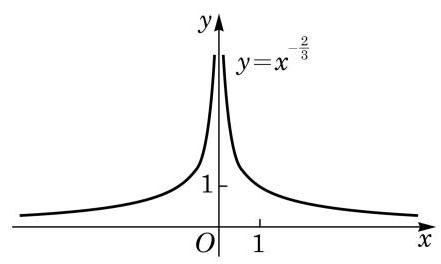
\includegraphics[max width=0.3\textwidth]{images/bo_d7fr3gc91nqc7381iccg_92_801_1120_441_264_0.jpg}
\end{center}
\hspace*{3em} 

图 4-1-3

由例 1,可知幂函数 \(y = {x}^{-\frac{2}{3}}\) 的定义域为不等于 0 的一切实数. 若点 \(\left( {{x}_{0},{y}_{0}}\right)\) 在幂函数 \(y = {x}^{-\frac{2}{3}}\) 的图像上,则有 \({y}_{0} = {x}_{0}^{-\frac{2}{3}}\) . 而点 \(\left( {{x}_{0},{y}_{0}}\right)\) 关于 \(y\) 轴的对称点易知是 \(\left( {-{x}_{0},{y}_{0}}\right)\) ,如图 4-1-4 所示. 由 \({y}_{0} = {x}_{0}^{-\frac{2}{3}}\) ,且 \({\left( -{x}_{0}\right) }^{-\frac{2}{3}} = \frac{1}{\sqrt[3]{{\left( -{x}_{0}\right) }^{2}}} = \frac{1}{\sqrt[3]{{x}_{0}^{2}}} = {x}_{0}^{-\frac{2}{3}}\) ,易知同时有 \({y}_{0} = {\left( -{x}_{0}\right) }^{-\frac{2}{3}}\) ,从而点 \(\left( {-{x}_{0},{y}_{0}}\right)\) 也落在幂函数 \(y = {x}^{-\frac{2}{3}}\) 的图像上. 这说明幂函数 \(y = {x}^{-\frac{2}{3}}\) 的图像关于 \(y\) 轴成轴对称.

\begin{center}
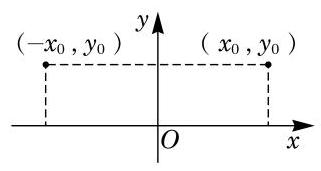
\includegraphics[max width=0.2\textwidth]{images/bo_d7fr3gc91nqc7381iccg_92_191_1594_321_171_0.jpg}
\end{center}
\hspace*{3em} 

图 4-1-4

\section*{练习 4.1(1)}

1. 若幂函数 \(y = {x}^{a}\) 的图像经过点 \(\left( {3,\sqrt{3}}\right)\) ,求此幂函数的表达式.

2. 求下列函数的定义域, 并作出它们的大致图像:





(1) \(y = {x}^{\frac{1}{3}}\) ；

(2) \(y = {x}^{-\frac{1}{2}}\) ；

(3) \(y = {x}^{\frac{4}{3}}\) .

3. 若幂函数 \(y = {x}^{-{m}^{2} + {2m} + 3}\) ( \(m\) 为整数) 的定义域为 \(\mathbf{R}\) ,求 \(m\) 的值.

\section*{2 幂函数的性质}

由前述,不管指数 \(a\) 取何值,当 \(x > 0\) 时,幂函数 \(y = {x}^{a}\) 总是有定义的,且其函数值 \(y > 0\) . 这说明,幂函数 \(y = {x}^{a}\) 在第一象限总有图像,其图像随指数 \(a\) 取值的不同,可分为两种情况.

(1) \(a > 0\) 的情况. 此时观察幂函数 \(y = {x}^{a}\) 在第一象限的图像,不难发现,当指数 \(0 < a < 1\) 时,相应的图像类似图 4-1-5 中 \(y = {x}^{\frac{1}{2}}\) 的图像; 当指数 \(a > 1\) 时,相应的图像类似图 4-1-5 中 \(y = {x}^{3}\) 的图像; 而当 \(a = 1\) 时,幂函数 \(y = x\) 的图像是一条经过原点的直线.

\HRule

当 \(a = 0\) 时,幂函数 \(y = {x}^{0} = 1\left( {x \neq  0}\right)\) 的图像是平行于 \(x\) 轴、 并在 \(x\) 轴上方一个单位的一条直线(除去点 (0,1)).

当 \(a = 1\) 时,幂函数 \(y = x\) 的图像是经过原点的一条直线.

\HRule

\begin{center}
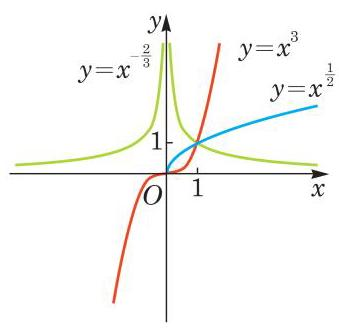
\includegraphics[max width=0.2\textwidth]{images/bo_d7fr3gc91nqc7381iccg_93_1131_1260_339_329_0.jpg}
\end{center}
\hspace*{3em} 

图 4-1-5

观察图 4-1-5 所示的幂函数 \(y = {x}^{a}\left( {a > 0}\right)\) 在第一象限的图像,可发现图像由左至右是上升的,也就是说,随着自变量 \(x\) 的不断增大,函数值 \(y\) 也不断增大. 这是因为当 \(a > 0\) 时,若 \({x}_{2} > {x}_{1} > 0\) ,则 \(\frac{{x}_{2}}{{x}_{1}} > 1\) ,从而由幂的基本不等式,得

\[
{\left( \frac{{x}_{2}}{{x}_{1}}\right) }^{a} > 1
\]

即 \({x}_{2}^{a} > {x}_{1}^{a}\) . 这说明在区间 \(\left( {0, + \infty }\right)\) 上幂函数 \(y = {x}^{a}\left( {a > 0}\right)\) 的函数值 \(y\) 随着 \(x\) 的 (严格) 增大而 (严格) 增大. 此时称幂函数 \(y = {x}^{a} \; \left( {a > 0}\right)\) 在区间 \(\left( {0, + \infty }\right)\) 上是严格增函数.

(2) \(a < 0\) 的情况. 此时幂函数 \(y = {x}^{a}\) 在第一象限的图像类似图 4-1-5 中 \(y = {x}^{-\frac{2}{3}}\) 的图像. 该图像由左至右是下降的,也就是说,在区间 \(\left( {0, + \infty }\right)\) 上幂函数 \(y = {x}^{a}\left( {a < 0}\right)\) 的函数值 \(y\) 随着 \(x\) 的 (严格) 增大而 (严格) 减小. 此时称幂函数 \(y = {x}^{a}\left( {a < 0}\right)\) 在区间 \(\left( {0, + \infty }\right)\) 上是严格减函数.

因为 \({1}^{a} = 1\) ,所以无论 \(a > 0\) 还是 \(a < 0\) ,幂函数的图像均经过点 \(\left( {1,1}\right)\) .



例 4 比较下列各题中两个数的大小:

(1) \({2.5}^{-2}\) 与 \({1.8}^{-2}\) ；

(2) \({1.32}^{\frac{4}{5}}\) 与 \({\left( -\sqrt{2}\right) }^{\frac{4}{5}}\) .

解 (1) 考虑幂函数 \(y = {x}^{-2}\) . 由于指数小于 0 的幂函数在区间 \(\left( {0, + \infty }\right)\) 上是严格减函数,因此 \({2.5}^{-2} < {1.8}^{-2}\) .

(2)考虑幂函数 \(y = {x}^{\frac{4}{5}}\) . 由于

\[
{\left( -\sqrt{2}\right) }^{\frac{4}{5}} = \sqrt[5]{{\left( -\sqrt{2}\right) }^{4}} = \sqrt[5]{{\left( \sqrt{2}\right) }^{4}} = {\sqrt{2}}^{\frac{4}{5}},
\]

而指数大于 0 的幂函数在区间 \(\left( {0, + \infty }\right)\) 上是严格增函数,因此

\[
{1.32}^{\frac{4}{5}} < {\sqrt{2}}^{\frac{4}{5}},
\]

故

\[
{1.32}^{\frac{4}{5}} < {\left( -\sqrt{2}\right) }^{\frac{4}{5}}.
\]

下面我们研究一些函数图像之间的关系.

例 5 已知函数 \(y = \frac{1}{x}\) 和 \(y = \frac{1}{x - 2}\) ,说明这两个函数图像之间的关系, 并在同一平面直角坐标系中作出它们的大致图像.

解 在幂函数 \(y = \frac{1}{x}\) 的图像上任取一点 \(P\left( {a,\frac{1}{a}}\right)\) ,易得点 \({P}^{\prime }\left( {a + 2,\frac{1}{a}}\right)\) 一定在函数 \(y = \frac{1}{x - 2}\) 的图像上,而将点 \(P\) 向右平移 2 个单位就与点 \({P}^{\prime }\) 重合. 反之亦然. 因此,将函数 \(y = \frac{1}{x}\) 的图像向右平移 2 个单位就得到函数 \(y = \frac{1}{x - 2}\) 的图像. 反之,将函数 \(y = \frac{1}{x - 2}\) 的图像向左平移 2 个单位就得到函数 \(y = \frac{1}{x}\) 的图像,如图 4-1-6 所示.

\begin{center}
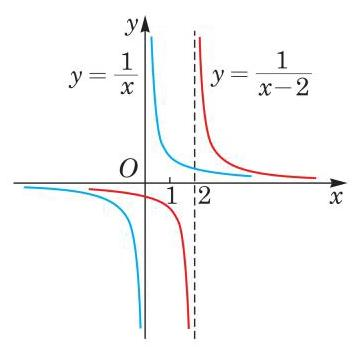
\includegraphics[max width=0.3\textwidth]{images/bo_d7fr3gc91nqc7381iccg_94_169_1303_352_348_0.jpg}
\end{center}
\hspace*{3em} 

图 4-1-6

例 6 已知函数 \(y = \frac{1}{x - 2}\) 和 \(y = \frac{x - 1}{x - 2}\) ,说明这两个函数图像之间的关系, 并在同一平面直角坐标系中作出它们的大致图像.

解 将 \(y = \frac{x - 1}{x - 2}\) 整理变形,得 \(y = 1 + \frac{1}{x - 2}\) . 若点 \(Q\left( {a,\frac{1}{a - 2}}\right)\) 在函数 \(y = \frac{1}{x - 2}\) 的图像上,则点 \({Q}^{\prime }\left( {a,1 + \frac{1}{a - 2}}\right)\) 就一定在函数

\section*{}



4.1 \(y = 1 + \frac{1}{x - 2}\) 的图像上,即将点 \(Q\) 向上平移 1 个单位就与点 \({Q}^{\prime }\) 重合. 反之亦然. 因此,将函数 \(y = \frac{1}{x - 2}\) 的图像向上平移 1 个单位就得到函数 \(y = \frac{x - 1}{x - 2}\) 的图像. 反之,将函数 \(y = \frac{x - 1}{x - 2}\) 的图像向下平移 1 个单位就得到函数 \(y = \frac{1}{x - 2}\) 的图像,如图 4-1-7 所示.

\begin{center}
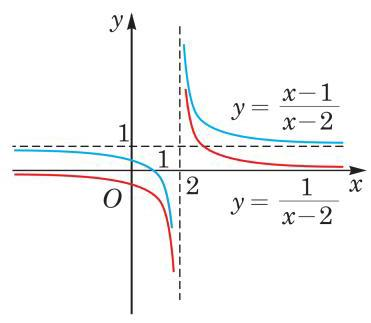
\includegraphics[max width=0.3\textwidth]{images/bo_d7fr3gc91nqc7381iccg_95_1120_232_371_323_0.jpg}
\end{center}
\hspace*{3em} 

图 4-1-7

\section*{练习 4.1(2)}

1. ( 1 )已知函数 \(y = {x}^{\frac{2}{3}}\) 和 \(y = {\left( x - 1\right) }^{\frac{2}{3}}\) ，说明这两个函数图像之间的关系，并在同一平面直角坐标系中作出它们的大致图像;

(2)已知函数 \(y = {x}^{\frac{2}{3}}\) 和 \(y = {x}^{\frac{2}{3}} + 1\) ，说明这两个函数图像之间的关系，并在同一平面直角坐标系中作出它们的大致图像.

2. 比较下列各题中两个数的大小:

(1) \({2.5}^{-3}\) 与 \({3.1}^{-3}\) ； (2) \({1.7}^{\frac{3}{2}}\) 与 \({1.6}^{\frac{3}{2}}\) .

3. 作出函数 \(y = \frac{-x - 1}{x + 2}\) 的大致图像.

\section*{习题 4.1}

\section*{A 组}

1. 若幂函数 \(y = {x}^{a}\) 的图像经过点 \(\left( {\sqrt[4]{3},3}\right)\) ,求此幂函数的表达式.

2. 求下列函数的定义域, 并作出它们的大致图像:

(1) \(y = {x}^{\frac{1}{5}}\) ； (2) \(y = {x}^{-2}\) ； (3) \(y = {x}^{-\frac{3}{4}}\) .

3. 在固定压力差(压力差为常数)的前提下，当气体通过圆形管道时，其速率 \(v\) (单位: \(\left. {{\mathrm{{cm}}}^{3}/\mathrm{s}}\right)\) 与管道半径 \(r\) (单位: \(\mathrm{{cm}}\) ) 的四次方成正比. 若在半径为 \(3\mathrm{\;{cm}}\) 的管道中,某气体的速率为 \({400}{\mathrm{\;{cm}}}^{3}/\mathrm{s}\) ,求该气体通过半径为 \(5\mathrm{\;{cm}}\) 的管道时的速率. (结果精确到 \(1{\mathrm{\;{cm}}}^{3}/\mathrm{s}\) )

4. 比较下列各题中两个数的大小:

(1) \({3.1}^{-\frac{1}{2}}\) 与 \({3.2}^{-\frac{1}{2}}\) ； (2) \({\left( a + 2\right) }^{\frac{1}{3}}\) 与 \({a}^{\frac{1}{3}}\) .

5. 下列幂函数在区间 \(\left( {0, + \infty }\right)\) 上是严格增函数,且图像关于原点成中心对称的是\_\_\_\_\_(请填入全部正确的序号).

 \circled{1}  \(y = {x}^{\frac{1}{2}}\) ；  \circled{2}  \(y = {x}^{\frac{1}{3}}\) ；  \circled{3}  \(y = {x}^{\frac{2}{3}}\) ；  \circled{4}  \(y = {x}^{-\frac{1}{3}}\) .

6. 作出函数 \(y = \frac{x - 1}{x + 2}\) 的大致图像.

\section*{B 组}

1. 填空题:

(1)幂函数 \(y = {x}^{n\left( {n + 1}\right) }\) ( \(n\) 为正整数)的图像一定经过\_\_\_\_\_象限.

(2)若幂函数 \(y = {x}^{s}\) 在 \(0 < x < 1\) 时的图像位于直线 \(y = x\) 的上方,则 \(s\) 的取值范围是\_\_\_\_\_.

2. 下列命题中, 正确的是 ( )

A. 当 \(n = 0\) 时,函数 \(y = {x}^{n}\) 的图像是一条直线;

B. 幂函数 \(y = {x}^{n}\) 的图像都经过 \(\left( {0,0}\right)\) 和 \(\left( {1,1}\right)\) 两个点;

C. 若幂函数 \(y = {x}^{n}\) 的图像关于原点成中心对称,则 \(y = {x}^{n}\) 在区间 \(\left( {-\infty ,0}\right)\) 上是严格增函数;

D. 幂函数的图像不可能在第四象限.

3. 写出一个图像经过第一、第二象限但不经过原点的幂函数的表达式.

4. 已知函数 \(y = \frac{{ax} + 1}{x + 2}\) (常数 \(a \in  \mathbf{Z}\) ). 问: 是否存在整数 \(a\) ,使该函数在区间 \(\lbrack 1, + \infty )\) 上是严格减函数，并且函数值不恒为负？若存在，求出所有符合条件的 \(a\) ；若不存在，请说明理由.



\section*{4.2 指数函数}

\section*{1 指数函数的定义与图像}

研究这样一个问题: 一张纸对折一次, 由 1 层变为 2 层, 再对折一次,由 2 层变为 4 层, \(\cdots \cdots\) ,对折 \(x\) 次后,层数 \(y\) 与对折次数 \(x\) 的函数关系为 \(y = {2}^{x}\) .

将幂的底数 \(a\) 固定,指数用变量 \(x\) 代替,研究幂 \({a}^{x}\) 随 \(x\) 变化而变化的规律, 即用

\[
y = {a}^{x}
\]

来描述 \(y\) 与 \(x\) 之间的关系,就得到指数函数.

这里首先要假设 \(a > 0\) ,以保证对所有的实数 \(x,{a}^{x}\) 都有意义. 还要假设 \(a \neq  1\) ,因为如果 \(a = 1,{a}^{x}\) 就恒等于 1,这种极为特殊的情况不必专门研究.

定义 当底数 \(a\) 固定,且 \(a > 0,a \neq  1\) 时,等式

\[
y = {a}^{x}
\]

确定了变量 \(y\) 随变量 \(x\) 变化的规律,称为底为 \(a\) 的指数函数 (exponential function).

因为对所有实数 \(x,{a}^{x}\) 都是有意义的,所以指数函数的定义域是全体实数.

在平面直角坐标系中,满足 \(y = {a}^{x}\left( {a > 0\text{ 且 }a \neq  1}\right)\) 的一切点 \(\left( {x,y}\right)\) 构成指数函数 \(y = {a}^{x}\left( {a > 0\text{ 且 }a \neq  1}\right)\) 的图像.

例 1 若指数函数 \(y = {a}^{x}\left( {a > 0\text{ 且 }a \neq  1}\right)\) 的图像经过点 \(\left( {2,9}\right)\) ,求该指数函数的表达式.

解 因为指数函数 \(y = {a}^{x}\left( {a > 0\text{ 且 }a \neq  1}\right)\) 的图像经过点 \(\left( {2,9}\right)\) ,所以 \(9 = {a}^{2}\left( {a > 0\text{ 且 }a \neq  1}\right)\) ,解得 \(a = 3\) .

因此,该指数函数的表达式为 \(y = {3}^{x}\) .



\HRule

规定指数函数底 \(a > 0\) 且 \(a \neq  1\) .

\HRule



例 2 分别作出指数函数 \(y = {2}^{x}\) 及 \(y = {3}^{x}\) 的大致图像.

解 先在相应的图像上取一些特殊的点.

由 \({2}^{-2} = \frac{1}{4},{2}^{-1} = \frac{1}{2},{2}^{0} = 1,{2}^{1} = 2,{2}^{2} = 4\) ,可知指数函数 \(y = {2}^{x}\) 的图像必经过下面的点:

\[
\left( {-2,\frac{1}{4}}\right) \text{ 、 }\left( {-1,\frac{1}{2}}\right) \text{ 、 }\left( {0,1}\right) \text{ 、 }\left( {1,2}\right) \text{ 、 }\left( {2,4}\right) .
\]

再使用计算器多采集一些点, 可以粗略地作出其图像.

\begin{center}
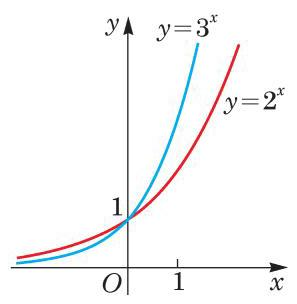
\includegraphics[max width=0.2\textwidth]{images/bo_d7fr3gc91nqc7381iccg_98_200_696_297_304_0.jpg}
\end{center}
\hspace*{3em} 

图 4-2-1

由 \({3}^{-2} = \frac{1}{9},{3}^{-1} = \frac{1}{3},{3}^{0} = 1,{3}^{1} = 3,{3}^{2} = 9\) ,可知指数函数 \(y = {3}^{x}\) 的图像必经过下面的点:

\[
\left( {-2,\frac{1}{9}}\right) \text{ 、 }\left( {-1,\frac{1}{3}}\right) \text{ 、 }\left( {0,1}\right) \text{ 、 }\left( {1,3}\right) \text{ 、 }\left( {2,9}\right) .
\]

再使用计算器多采集一些点, 可以粗略地作出其图像.

我们把这两个图像放在同一个平面直角坐标系中以便观察比较, 如图4-2-1所示.

例 3 作出指数函数 \(y = {\left( \frac{1}{2}\right) }^{x}\) 的大致图像.

\begin{center}
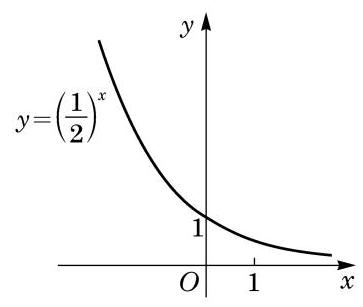
\includegraphics[max width=0.3\textwidth]{images/bo_d7fr3gc91nqc7381iccg_98_164_1201_363_307_0.jpg}
\end{center}
\hspace*{3em} 

图 4-2-2

解 由 \({\left( \frac{1}{2}\right) }^{-2} = 4,{\left( \frac{1}{2}\right) }^{-1} = 2,{\left( \frac{1}{2}\right) }^{0} = 1,{\left( \frac{1}{2}\right) }^{1} = \frac{1}{2}\) , \({\left( \frac{1}{2}\right) }^{2} = \frac{1}{4}\) ,可知指数函数 \(y = {\left( \frac{1}{2}\right) }^{x}\) 的图像必经过下面的点:

\[
\left( {-2,4}\right) \text{ 、 }\left( {-1,2}\right) \text{ 、 }\left( {0,1}\right) \text{ 、 }\left( {1,\frac{1}{2}}\right) \text{ 、 }\left( {2,\frac{1}{4}}\right) .
\]

类似地, 可以粗略作出其相应的图像, 如图 4-2-2 所示.

\section*{练习 4.2(1)}

1. 判断下列函数哪些是指数函数, 哪些是幂函数:

(1) \(y = x\) ； (2) \(y = {x}^{3}\) ； (3) \(y = {\mathrm{e}}^{x}\) ；

(4) \(y = \sqrt[3]{x}\) ； (5) \(y = {2}^{-x}\) ; (6) \(y = {2}^{x}\) .

2. 求下列函数的定义域:

(1) \(y = {3}^{x}\) ； (2) \(y = {3}^{\frac{1}{x - 2}}\) .

3. 在同一平面直角坐标系中分别作出下列函数的大致图像:

(1) \(y = {4}^{x}\) ； (2) \(y = {\left( \frac{1}{4}\right) }^{x}\) .





\section*{2 指数函数的性质}

由前述两种指数函数的图像可见,它们的图像均在 \(x\) 轴的上方. 这是因为当 \(a > 0\) 时,对一切实数 \(x,{a}^{x}\) 均大于 0 . 因此,我们有如下的性质:

指数函数 \(y = {a}^{x}\left( {a > 0\text{ 且 }a \neq  1}\right)\) 的函数值恒大于 0 .

因为 \({a}^{0} = 1\) ,所以指数函数 \(y = {a}^{x}\) 的图像均经过点 \(\left( {0,1}\right)\) . 因此，我们有如下的性质:

指数函数 \(y = {a}^{x}\left( {a > 0\text{ 且 }a \neq  1}\right)\) 的图像都经过定点 \(\left( {0,1}\right)\) .

由例 2 和例 3 可见,指数函数 \(y = {a}^{x}\) 的图像可分为两种情况.

(1) \(a > 1\) 的情况. 此时指数函数 \(y = {a}^{x}\) 的图像类似图4-2-1 中 \(y = {2}^{x}\) 的图像,当 \(x > 0\) 时,函数值大于 1,其图像在直线 \(y = 1\) 的上方; 而当 \(x < 0\) 时,函数值小于 1 且大于 0,其图像在直线 \(y = 1\) 的下方,且位于 \(x\) 轴的上方.

(2) \(0 < a < 1\) 的情况. 此时指数函数 \(y = {a}^{x}\) 的图像类似图 4-2-2中 \(y = {\left( \frac{1}{2}\right) }^{x}\) 的图像,当 \(x > 0\) 时,函数值小于 1 且大于 0, 其图像在直线 \(y = 1\) 的下方,且位于 \(x\) 轴的上方; 而当 \(x < 0\) 时, 函数值大于 1,其图像在直线 \(y = 1\) 的上方.

\begin{center}
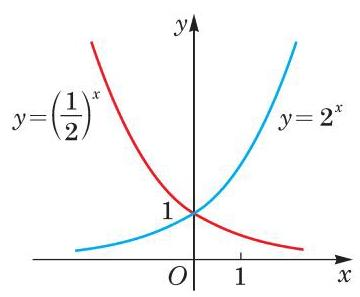
\includegraphics[max width=0.3\textwidth]{images/bo_d7fr3gc91nqc7381iccg_99_1125_1403_360_297_0.jpg}
\end{center}
\hspace*{3em} 

图 4-2-3

这两种情况在同一平面直角坐标系中的图像如图 4-2-3 所示. 易见这两个指数函数 \(y = {2}^{x}\) 与 \(y = {\left( \frac{1}{2}\right) }^{x}\) 的图像关于 \(y\) 轴对称.

一般地说, 由指数幂的运算性质

\[
{a}^{{x}_{0}} = {\left( {a}^{-1}\right) }^{-{x}_{0}},
\]

容易看到: 若 \(\left( {{x}_{0},{y}_{0}}\right)\) 为指数函数 \(y = {a}^{x}\) 图像上的一点,则 \(\left( {-{x}_{0},{y}_{0}}\right)\) 必为指数函数 \(y = {\left( {a}^{-1}\right) }^{x}\) 图像上的点,反之亦然. 由于 \(\left( {{x}_{0},{y}_{0}}\right)\) 及 \(\left( {-{x}_{0},{y}_{0}}\right)\) 两点关于 \(y\) 轴对称,因此指数函数 \(y = {a}^{x}\) 及 \(y = {\left( {a}^{-1}\right) }^{x}\) 的图像必关于 \(y\) 轴对称.

\HRule

指数函数 \(y = {a}^{x}\) 的图像与指数函数 \(y = {\left( {a}^{-1}\right) }^{x}\) 的图像关于 \(y\) 轴对称.

\HRule

观察图 4-2-1 中两个指数函数的图像, 它们的底都大于 1, 图像由左至右是上升的,也就是说,随着自变量 \(x\) 的不断增大, 函数值 \(y\) 也不断增大,这点也可以证明如下:

\section*{}

当 \(a > 1\) 时,若 \({x}_{2} > {x}_{1}\) ,则 \({x}_{2} - {x}_{1} > 0\) ,由幂的基本不等式有

\[
{a}^{{x}_{2} - {x}_{1}} > 1,
\]

即 \({a}^{{x}_{2}} > {a}^{{x}_{1}}\) . 此时,称指数函数 \(y = {a}^{x}\left( {a > 1}\right)\) 在 \(\mathbf{R}\) 上是严格增函数,即函数值 \(y\) 随着 \(x\) 的 (严格) 增大而 (严格) 增大.

同理可证: 当 \(0 < a < 1\) 时,指数函数 \(y = {a}^{x}\) 在 \(\mathbf{R}\) 上是严格减函数.

因此，我们有

指数函数的单调性 当 \(a > 1\) 时,指数函数 \(y = {a}^{x}\) 在 \(\mathbf{R}\) 上是严格增函数; 当 \(0 < a < 1\) 时,指数函数 \(y = {a}^{x}\) 在 \(\mathbf{R}\) 上是严格减函数.

指数函数的图像与性质可总结见下表 4-1:

表 4-1

\begin{center}
\adjustbox{max width=\textwidth}{
\begin{tabular}{|c|c|c|}
\hline
\(y = {a}^{x}\) & \(a > 1\) & \(0 < a < 1\) \\
\cline{1-3}
图像 & 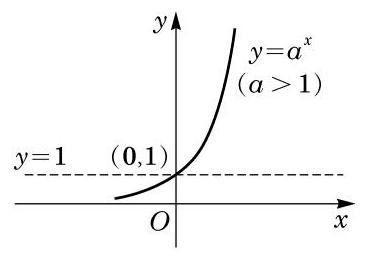
\includegraphics[max width=0.3\textwidth]{images/bo_d7fr3gc91nqc7381iccg_100_717_1085_365_257_0.jpg} & 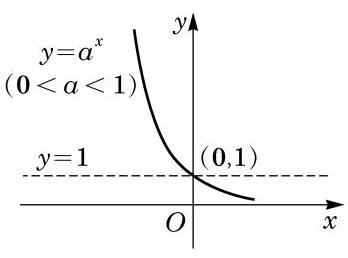
\includegraphics[max width=0.2\textwidth]{images/bo_d7fr3gc91nqc7381iccg_100_1130_1084_348_258_0.jpg} \\
\cline{1-3}
\multirow{3}{*}{图像特征} & \multicolumn{2}{|c|}{(1)图像都在 \(x\) 轴上方，无限趋近于 \(x\) 轴，但永不相交.} \\
\cline{2-3}
 & \multicolumn{2}{|c|}{(2)过点 \(\left( {0,1}\right)\) .} \\
\cline{2-3}
 & (3)由左至右图像上升. & (3)由左至右图像下降. \\
\cline{1-3}
\multirow{3}{*}{函数性质} & \multicolumn{2}{|c|}{(1)定义域为 \(\mathbf{R}\) ，函数值恒正.} \\
\cline{2-3}
 & \multicolumn{2}{|c|}{(2)当 \(x = 0\) 时， \(y = 1\) .} \\
\cline{2-3}
 & (3)在 \(\mathbf{R}\) 上是严格增函数. & (3)在 \(\mathbf{R}\) 上是严格减函数. \\
\cline{1-3}
\hline
\end{tabular}
}
\end{center}

例 4 利用指数函数的性质, 比较下列各题中两个数的大小:

(1)1. \({7}^{2.5}\) 与 \({1.7}^{3}\) ；

(2) \({\left( \frac{3}{4}\right) }^{\frac{1}{6}}\) 与 \({\left( \frac{4}{3}\right) }^{-\frac{1}{5}}\) ；\_\_\_\_\_

(3) \({a}^{\frac{1}{2}}\) 与 \({a}^{\frac{1}{3}}\left( {a > 0\text{ 且 }a \neq  1}\right)\) .

解 (1) 由于底数 \(a\) 大于 1 的指数函数 \(y = {a}^{x}\) 在 \(\mathbf{R}\) 上是严



格增函数,因此 \({1.7}^{2.5} < {1.7}^{3}\) .

(2)由于 \({\left( \frac{4}{3}\right) }^{-\frac{1}{5}} = {\left( \frac{3}{4}\right) }^{\frac{1}{5}}\) ，且底数 \(a\) 小于 1 大于 0 的指数函数 \(y = {a}^{x}\) 在 \(\mathbf{R}\) 上是严格减函数,因此

\[
{\left( \frac{3}{4}\right) }^{\frac{1}{6}} > {\left( \frac{4}{3}\right) }^{-\frac{1}{5}}.
\]

(3)当 \(0 < a < 1\) 时，指数函数 \(y = {a}^{x}\) 在 \(\mathbf{R}\) 上是严格减函数， 故 \({a}^{\frac{1}{2}} < {a}^{\frac{1}{3}}\) ;

当 \(a > 1\) 时,指数函数 \(y = {a}^{x}\) 在 \(\mathbf{R}\) 上是严格增函数,故 \({a}^{\frac{1}{2}} > {a}^{\frac{1}{3}}\) .

例 5 求下列不等式的解集:

(1) \({3}^{x} > \frac{1}{27}\) ；

(2) \({a}^{{x}^{2} - {2x} + 3} > {a}^{6}\left( {0 < a < 1}\right)\) .

解 (1) 将 \(\frac{1}{27}\) 写成 \({3}^{-3}\) ，因为指数函数 \(y = {3}^{x}\) 在 \(\mathbf{R}\) 上是严格增函数,所以 \(x >  - 3\) . 故原不等式的解集为 \(\left( {-3, + \infty }\right)\) .

(2)当 \(0 < a < 1\) 时，指数函数 \(y = {a}^{x}\) 在 \(\mathbf{R}\) 上是严格减函数， 因此有 \({x}^{2} - {2x} + 3 < 6\) ,整理得 \({x}^{2} - {2x} - 3 < 0\) ,解得 \(- 1 < x < 3\) . 故原不等式的解集为 \(\left( {-1,3}\right)\) .

\section*{练习 4.2(2)}

1. 比较下列各题中两个数的大小:

(1) \({1.4}^{0.3}\) 与 \({1.4}^{0.4}\) ；

(2) \({0.3}^{1.4}\) 与 \({0.3}^{1.5}\) ；

(3) \({a}^{-{3.14}}\) 与 \({\left( \frac{1}{a}\right) }^{\pi }\left( {a > 0\text{ 且 }a \neq  1}\right)\) .

2. 已知 \(a > 0\) 且 \(a \neq  1\) . 若 \(m > n\) ,且 \({a}^{m} < {a}^{n}\) ,求实数 \(a\) 的取值范围.

3. 求下列不等式的解集:

(1) \({3}^{x} > {3}^{0.5}\) ； (2) \({0.2}^{x} < {25}\) .

例 6 已知指数函数 \(y = {a}^{x}\left( {a > 1}\right)\) 在区间 \(\left\lbrack  {1,2}\right\rbrack\) 上的最大值比最小值大 \(\frac{a}{3}\) ,求实数 \(a\) 的值.

解 当 \(a > 1\) 时,指数函数 \(y = {a}^{x}\) 在区间 \(\left\lbrack  {1,2}\right\rbrack\) 上是严格增函数. 所以,在区间 \(\left\lbrack  {1,2}\right\rbrack\) 上,当 \(x = 2\) 时,该指数函数取到最大值

 \({a}^{2}\) ; 当 \(x = 1\) 时,该指数函数取到最小值 \(a\) . 由题意,得 \({a}^{2} - a = \frac{a}{3}\) , 解得 \(a = \frac{4}{3}\) .

指数函数在生产实际和科学研究中有很多应用. 银行存款和贷款、GDP 的增长、人口增长等都可能涉及指数函数. 我们用以下的例子来体会“指数增长”.

例 7 统计资料显示: 某外来入侵物种现有种群数量为 \(k\) ,若有理想的外部环境条件,该物种的年平均增长率约为 20\%. 试建立该物种的种群数量增长模型, 并预测 30 年后该物种的种群数量约为现有种群数量的多少倍. (结果精确到个位)

解 设经过 1 年后, 该种群数量为

\[
{y}_{1} = k + k \cdot  {20}\%  = k\left( {1 + {20}\% }\right) ;
\]

经过 2 年后, 该种群数量为

\[
{y}_{2} = k\left( {1 + {20}\% }\right)  + k\left( {1 + {20}\% }\right)  \cdot  {20}\%
\]

\[
= k{\left( 1 + {20}\% \right) }^{2}\text{ ; }
\]

\HRule

当 \(a > 1\) 时,不仅 \({a}^{x}\) 随着 \(x\) 的增长而增长,且因为 \({a}^{x + 1} - {a}^{x} \; = {a}^{x}\left( {a - 1}\right)\) ,随着 \(x\) 的增长, \({a}^{x}\) 增长得越来越快. 这就是所谓的“指数增长”.

\HRule

......

以此类推,经过 \(n\) ( \(n\) 为正整数) 年后,该种群数量为 \({y}_{n} = \; k{\left( 1 + {20}\% \right) }^{n}\) .

当 \(n = {30}\) 时,该种群数量为 \({y}_{30} = k{\left( 1 + {20}\% \right) }^{30} \approx  {237k}\) .

因此, 若不加控制, 该种群的数量在 30 年之后约为现在的 237 倍, 从而可能极大地破坏当地生态系统的稳定, 这说明指数函数可以用于预测种群数量, 便于及早进行干预.

\section*{练习 4.2(3)}

1. 已知指数函数 \(y = {a}^{x}\left( {0 < a < 1}\right)\) 在区间 \(\left\lbrack  {1,2}\right\rbrack\) 上的最大值比最小值大 \(\frac{a}{3}\) ,求实数 \(a\) 的值.

2. 某服装店对原价分别为 175 元和 200 元的甲乙两种服装搞促销活动, 规定甲服装每天降价 5\%，直到其售完为止；乙服装每天降价 7\%，直到其售完为止. 假设两种服装在 10 天内均没有售完, 几天后甲服装的售价将高于乙服装的售价?



\section*{习题 4.2}

\section*{A 组}

1. 下列函数是指数函数的序号为\_\_\_\_\_. (请填入全部正确的序号)

 \circled{1}  \(y = {\left( -4\right) }^{x}\) ；  \circled{2}  \(y = {\left( \frac{1}{4}\right) }^{x}\) ；  \circled{3}  \(y = {4}^{x}\) ；  \circled{4}  \(y = {x}^{-4}\) ；  \circled{5}  \(y = {\left( \sqrt{4}\right) }^{x}\) .

2. 求下列函数的定义域:

(1) \(y = {2}^{\sqrt{3 - x}}\) ； (2) \(y = {0.1}^{\frac{1}{x}}\) .

3. 在同一直角坐标系中作出下列函数的大致图像, 并指出这些函数图像间的关系:

(1) \(y = {\left( \frac{3}{2}\right) }^{x}\) ; (2) \(y = {\left( \frac{2}{3}\right) }^{x}\) ； (3) \(y = {\left( \frac{2}{3}\right) }^{x} - 1\) .

4. 已知指数函数 \(y = {\left( m - 2\right) }^{x}\) 在 \(\mathbf{R}\) 上是严格减函数,求实数 \(m\) 的取值范围.

5. 已知常数 \(a > 0\) 且 \(a \neq  1\) . 假设无论 \(a\) 取何值，函数 \(y = {a}^{2 - x}\) 的图像恒经过一个定点， 求此定点的坐标.

6. 比较下列各题中两个数的大小:

(1) \({1.2}^{2.6}\) 和 \({1.2}^{2.61}\) ；

(2) \({\left( \sqrt{3}\right) }^{-\frac{1}{3}}\) 和 \({\left( \frac{\sqrt{3}}{3}\right) }^{\frac{1}{2}}\) .

7. 求下列不等式的解集:

(1) \({3}^{{x}^{2} - {2x} + 3} < {3}^{2x}\) ；

(2) \({\left( \frac{1}{3}\right) }^{\sqrt{x}} \leq  \frac{1}{81}\) .

8. 已知指数函数 \(y = {a}^{x}\left( {a > 0\text{ 且 }a \neq  1}\right)\) 在区间 \(\left\lbrack  {1,2}\right\rbrack\) 上的最大值与最小值之和等于 6, 求实数 \(a\) 的值.

9. 某公司去年购置平板电脑 50 台, 并计划从今年起, 新购置的平板电脑数将按每年 5\%的比例增长. 求从今年起的第 10 年新购置的平板电脑数. (结果精确到 1 台)

\section*{B 组}

1. 在同一平面直角坐标系中,指数函数 \(y = {a}^{x}\left( {a > 0\text{ 且 }a \neq  1}\right)\) 和一次函数 \(y = a\left( {x + 1}\right)\) 的图像关系可能是 ( )



\begin{center}
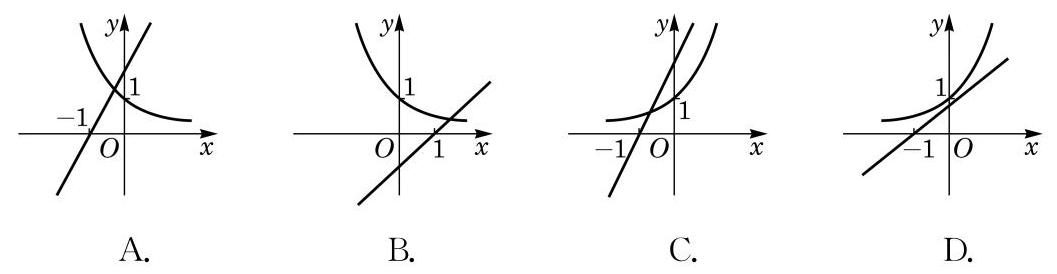
\includegraphics[max width=0.9\textwidth]{images/bo_d7fr3gc91nqc7381iccg_104_311_245_1057_274_0.jpg}
\end{center}
\hspace*{3em} 

(第 1 题)

\begin{center}
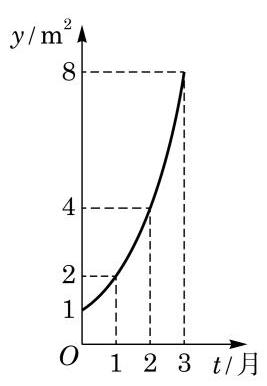
\includegraphics[max width=0.2\textwidth]{images/bo_d7fr3gc91nqc7381iccg_104_1232_595_267_386_0.jpg}
\end{center}
\hspace*{3em} 

(第 2 题)

2. 如图所示的是某池塘中的浮萍蔓延的面积 \(y\) (单位: \({\mathrm{m}}^{2}\) ) 与时间 \(t\) (单位: 月) 的关系: \(y = {a}^{t}\left( {a > 0\text{ 且 }a \neq  1}\right)\) . 以下结论:

 \circled{1}  这个指数函数的底数是 2 ;

 \circled{2}  第 5 个月时，浮萍的面积就会超过 30m \({}^{2}\) ；

 \circled{3}  浮萍面积从 \(4{\mathrm{\;m}}^{2}\) 到 \({12}{\mathrm{\;m}}^{2}\) 需要经过 1.5 个月；

 \circled{4}  浮萍每个月增加的面积都相等.

其中, 正确结论的序号是 ( )

A.  \circled{1}  \circled{2}  \circled{3} ; B.  \circled{1}  \circled{2}  \circled{3}  \circled{4} ；

C.  \circled{2}  \circled{3}  \circled{4} ; D.  \circled{1}  \circled{2} .

3. 若 \(x > 0\) 时,指数函数 \(y = {\left( {a}^{2} - 1\right) }^{x}\) 的值总大于 1,求实数 \(a\) 的取值范围.

4. 若 \(- 1 < x < 0\) ,比较 \({3}^{x},{3}^{-x}\) 及 \({3}^{2x}\) 的大小.

5. 设 \(a > 1\) ,若 \({a}^{{x}^{2} + {2x} + 1} < {a}^{2{x}^{2} - {3x} + 1}\) ,求实数 \(x\) 的取值范围.

6. 若函数 \(y = {5}^{x + 1} + m\) 的图像不经过第二象限,求实数 \(m\) 的取值范围.

\section*{4.3 对数函数}

\section*{1 对数函数的定义与图像}

我们已经学过幂函数及指数函数. 本节我们将利用对数来引入对数函数.

前面我们已经知道什么是正数 \(N\) 以 \(a\) 为底的对数 \({\log }_{a}N\) , 其中 \(a > 0\) 且 \(a \neq  1\) .

现在，将对数的底数 \(a\) 固定，而将真数 \(N\) 用变量 \(x\) 代替， 以研究对数的值 \({\log }_{a}x\) 随 \(x\) 变化而变化的规律. 用

\[
y = {\log }_{a}x
\]

来描述 \(y\) 与 \(x\) 的关系就是对数函数.

定义 当底数 \(a\) 固定,且 \(a > 0,a \neq  1\) 时, \(x\) 以 \(a\) 为底的对数

\[
y = {\log }_{a}x
\]

确定了变量 \(y\) 随变量 \(x\) 变化的规律,称为底为 \(a\) 的对数函数 (logarithmic function).

因为只有当 \(x > 0\) 时, \({\log }_{a}x\) 才有意义,所以对数函数的定义域是全体正数.

例 1 求下列函数的定义域:

(1) \(y = {\log }_{2}\left( {x - 1}\right)\) ；

(2) \(y = {\log }_{a}\left( {{x}^{2} - {4x} - 5}\right)\) (常数 \(a > 0\) 且 \(a \neq  1)\) .

解 (1) 当 \(x - 1 > 0\) ,即 \(x > 1\) 时,该函数才有意义,所以该函数的定义域是 \(\left( {1, + \infty }\right)\) .

(2)当 \({x}^{2} - {4x} - 5 > 0\) 时，该函数才有意义，而

\[
{x}^{2} - {4x} - 5 = \left( {x + 1}\right) \left( {x - 5}\right) ,
\]

不等式 \({x}^{2} - {4x} - 5 > 0\) 的解是 \(x <  - 1\) 或 \(x > 5\) ,所以该函数的定义域是 \(\left( {-\infty , - 1}\right)  \cup  \left( {5, + \infty }\right)\) .



\HRule

规定对数函数的底 \(a > 0\) 且 \(a \neq  1\) .

\HRule

前面已经看到, 函数图像是直观理解变量间关系的一个重要手段. 下面我们来考察对数函数 \(y = {\log }_{a}x\) 的图像及其性质,这里总假设 \(a > 0\) 且 \(a \neq  1\) .

在平面直角坐标系中,把满足 \(y = {\log }_{a}x\) 的一切点 \(\left( {x,y}\right)\) 描绘出来就构成对数函数 \(y = {\log }_{a}x\) 的图像. 像以前学习过的其他函数一样, 对数函数的图像也是一条曲线.

例 2 分别作出对数函数 \(y = {\log }_{2}x\) 及 \(y = {\log }_{3}x\) 的大致图像.

解 先取此图像上的一些特别的点,由 \({\log }_{2}\frac{1}{4} =  - 2\) , \({\log }_{2}\frac{1}{2} =  - 1,{\log }_{2}1 = 0,{\log }_{2}2 = 1,{\log }_{2}4 = 2\) ,所以对数函数 \(y = {\log }_{2}x\) 的图像必经过下面的点:

\[
\left( {\frac{1}{4}, - 2}\right) \text{ 、 }\left( {\frac{1}{2}, - 1}\right) \text{ 、 }\left( {1,0}\right) \text{ 、 }\left( {2,1}\right) \text{ 、 }\left( {4,2}\right) .
\]

再使用计算器多采集一些点, 就可以粗略地作出其图像.

\begin{center}
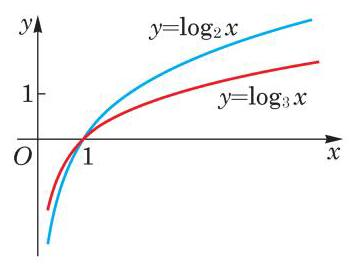
\includegraphics[max width=0.2\textwidth]{images/bo_d7fr3gc91nqc7381iccg_106_172_1138_350_267_0.jpg}
\end{center}
\hspace*{3em} 

图 4-3-1

因为 \({\log }_{3}\frac{1}{9} =  - 2,{\log }_{3}\frac{1}{3} =  - 1,{\log }_{3}1 = 0,{\log }_{3}3 = 1\) , \({\log }_{3}9 = 2\) ,所以对数函数 \(y = {\log }_{3}x\) 的图像必经过点:

\[
\left( {\frac{1}{9}, - 2}\right) \text{ 、 }\left( {\frac{1}{3}, - 1}\right) \text{ 、 }\left( {1,0}\right) \text{ 、 }\left( {3,1}\right) \text{ 、 }\left( {9,2}\right) .
\]

再多采集一些点, 就可以粗略地作出其图像.

我们把这两个图像放在同一个图上以便观察比较, 如图 4-3-1 所示.

\begin{center}
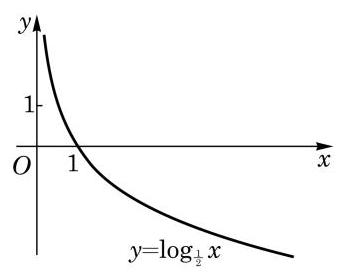
\includegraphics[max width=0.2\textwidth]{images/bo_d7fr3gc91nqc7381iccg_106_177_1595_340_275_0.jpg}
\end{center}
\hspace*{3em} 

图 4-3-2

例 3 作出对数函数 \(y = {\log }_{\frac{1}{2}}x\) 的大致图像.

解 因为 \({\log }_{\frac{1}{2}}\frac{1}{4} = 2,{\log }_{\frac{1}{2}}\frac{1}{2} = 1,{\log }_{\frac{1}{2}}1 = 0,{\log }_{\frac{1}{2}}2 =  - 1\) , \({\log }_{\frac{1}{2}}4 =  - 2\) ,所以该函数的图像经过下面的点:

\[
\left( {\frac{1}{4},2}\right) \text{ 、 }\left( {\frac{1}{2},1}\right) \text{ 、 }\left( {1,0}\right) \text{ 、 }\left( {2, - 1}\right) \text{ 、 }\left( {4, - 2}\right) .
\]

类似地, 可以粗略地作出其相应的图像, 如图 4-3-2 所示.

\section*{练习 4.3(1)}

1. 若对数函数 \(y = {\log }_{a}x\left( {a > 0\text{ 且 }a \neq  1}\right)\) 的图像经过点 \(\left( {4,2}\right)\) ,求此对数函数的表达式.



2. 求下列函数的定义域:

(1) \(y = {\log }_{2}\frac{2 + x}{1 - x}\) ；

(2) \(y = {\log }_{a}\left( {4 - {x}^{2}}\right)\) (常数 \(a > 0\) 且 \(a \neq  1\) ).

3. 在同一平面直角坐标系中作出 \(y = \lg x\) 及 \(y = {\log }_{0.1}x\) 的大致图像.

\section*{2 对数函数的性质}

由上述, 对数函数的图像可分为两种情况:

(1) \(a > 1\) 的情况. 此时，对数函数 \(y = {\log }_{a}x\) 的图像类似图 4-3-1中 \(y = {\log }_{2}x\) 的图像. 当 \(x > 1\) 时,函数值大于零,其图像在 \(x\) 轴的上方; 而当 \(0 < x < 1\) 时,函数值小于零,其图像在 \(x\) 轴的下方.

(2) \(0 < a < 1\) 的情况. 此时，对数函数图像类似图 4-3-2 中 \(y = {\log }_{\frac{1}{2}}x\) 的图像. 当 \(x > 1\) 时,函数值小于零,其图像在 \(x\) 轴的下方; 当 \(0 < x < 1\) 时,函数值大于零,其图像在 \(x\) 轴的上方.

这两种情况下的图像可见图 4-3-3 中两个对数函数 \(y = {\log }_{2}x\) 与 \(y = {\log }_{\frac{1}{2}}x\) 的图像. 它们看上去关于 \(x\) 轴对称,实际上也的确如此. 事实上, 由换底公式

\[
{\log }_{a}x =  - {\log }_{{a}^{-1}}x
\]

可得,在 \(0 < a < 1\) 时,底 \(a\) 小于 1 的对数函数 \(y = {\log }_{a}x\) 与底 \({a}^{-1}\) 大于 1 的对数函数 \(y = {\log }_{{a}^{-1}}x\) 恰相差一个符号,它们的图像关于 \(x\) 轴对称.

\HRule

函数 \(y = {\log }_{a}x\) 的图像与 \(y = {\log }_{{a}^{-1}}x\) 的图像关于 \(x\) 轴对称.

\HRule

\begin{center}
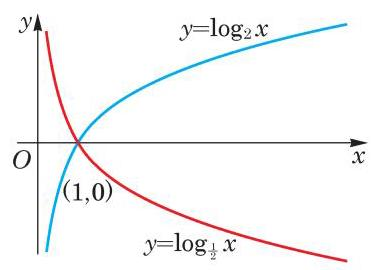
\includegraphics[max width=0.3\textwidth]{images/bo_d7fr3gc91nqc7381iccg_107_438_1599_373_270_0.jpg}
\end{center}
\hspace*{3em} 

图 4-3-3

因为 \({a}^{0} = 1\) 或者 \({\log }_{a}1 = 0\) ,所有指数函数 \(y = {a}^{x}\) 的图像均经过点 \(\left( {0,1}\right)\) ,而所有对数函数 \(y = {\log }_{a}x\) 的图像均经过点 \(\left( {1,0}\right)\) , 所以我们有如下的性质:

对数函数的图像总是经过点 \(\left( {1,0}\right)\) .



Q

因为 \(y = {\log }_{a}x\) 是 \({a}^{y} = x\) 的解,所以说对数运算是指数运算的一种逆运算. 作为函数,称对数函数 \(y = {\log }_{a}x\) 是指数函数 \(y = {a}^{x}\) 的反函数.

指数函数 \(y = {a}^{x}\) 的图像与其反函数即对数函数 \(y = {\log }_{a}x\) 的图像之间有什么关系呢? 它们的关系是: 对数函数 \(y = {\log }_{a}x\) 的图像与指数函数 \(y = {a}^{x}\) 的图像关于直线 \(y = x\) 是对称的. 这就是说,对数函数 \(y = {\log }_{a}x\) 的图像关于直线 \(y = x\) 对称的图像就是指数函数 \(y = {a}^{x}\) 的图像. 事实上,若点 \(\left( {{x}_{0},{y}_{0}}\right)\) 在对数函数 \(y = {\log }_{a}x\) 的图像上,就有 \({y}_{0} = {\log }_{a}{x}_{0}\) ,即 \({x}_{0} = {a}^{{y}_{0}}\) . 而点 \(\left( {{x}_{0},{y}_{0}}\right)\) 关于直线 \(y = x\) 的对称点就是 \(\left( {{y}_{0},{x}_{0}}\right)\) ,由于 \({x}_{0} = {a}^{{y}_{0}}\) , 因此 \(\left( {{y}_{0},{x}_{0}}\right)\) 必落在指数函数 \(y = {a}^{x}\) 的图像上. 反之亦然. 如图 4-3-4所示. Q

Q

\begin{center}
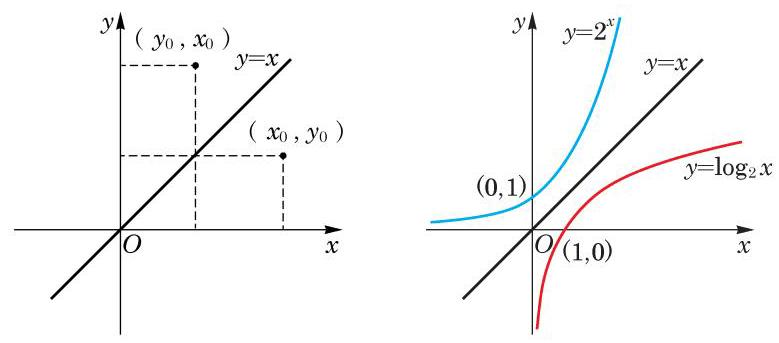
\includegraphics[max width=0.6\textwidth]{images/bo_d7fr3gc91nqc7381iccg_108_632_956_779_343_0.jpg}
\end{center}
\hspace*{3em} 

图 4-3-4

观察图 4-3-1 中的两个对数函数图像, 它们的底都大于 1, 且都是递增的,即在自变量 \(x\) 增大时,函数值 \(y\) 也增大. 这点在理论上也可以证明. 为此, 先证明下面的定理.

定理 当 \(a > 1,N > 1\) 时, \({\log }_{a}N > 0\) .

证明 用反证法证明. 如果 \(x = {\log }_{a}N \leq  0\) ,由指数函数的性质,就可得 \(N = {a}^{x} \leq  1\) ,与 \(N > 1\) 矛盾.

对数函数的单调性 当 \(a > 1\) 时,对数函数 \(y = {\log }_{a}x\) 在区间 \(\left( {0, + \infty }\right)\) 上是严格增函数; 当 \(0 < a < 1\) 时,对数函数 \(y = {\log }_{a}x\) 在区间 \(\left( {0, + \infty }\right)\) 上是严格减函数.

证明 当 \(a > 1\) 时,如果 \({x}_{2} > {x}_{1} > 0\) ,那么 \(\frac{{x}_{2}}{{x}_{1}} > 1\) ,由上面的



\HRule

反函数的概念将在下一章学习.

指数函数 \(y = {a}^{x}\) 的图像与其反函数对数函数 \(y = {\log }_{a}x\) 的图像关于直线 \(y = x\) 对称.

点 \(\left( {{x}_{0},{y}_{0}}\right)\) 关于直线 \(y = x\) 的对称点是 \(\left( {{y}_{0},{x}_{0}}\right)\) ,将在下一章证明.

此定理又称为对数的基本不等式.

\HRule

定理可得

\[
{\log }_{a}\frac{{x}_{2}}{{x}_{1}} > 0,
\]

即 \({\log }_{a}{x}_{2} > {\log }_{a}{x}_{1}\) . 这说明对数函数 \(y = {\log }_{a}x\) 在区间 \(\left( {0, + \infty }\right)\) 上是严格增函数,即 \(y\) 随着 \(x\) 的 (严格) 增大而 (严格) 增大.

当 \(0 < a < 1\) 时的结论,其证明留作课后练习.

关于对数函数 \(y = {\log }_{a}x\) 的图像与性质的总结见表 4-2.

表 4-2

\begin{center}
\adjustbox{max width=\textwidth}{
\begin{tabular}{|c|c|c|}
\hline
\(y = {\log }_{a}x\) & \(a > 1\) & \(0 < a < 1\) \\
\cline{1-3}
图像 & 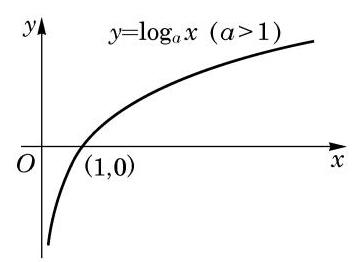
\includegraphics[max width=0.3\textwidth]{images/bo_d7fr3gc91nqc7381iccg_109_323_746_356_262_0.jpg} & 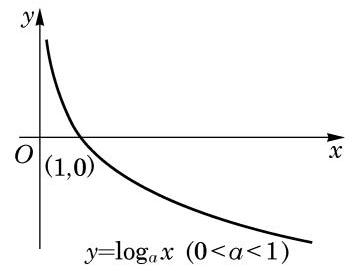
\includegraphics[max width=0.3\textwidth]{images/bo_d7fr3gc91nqc7381iccg_109_720_743_353_271_0.jpg} \\
\cline{1-3}
\multirow{3}{*}{图像特征} & \multicolumn{2}{|c|}{(1)图像都在 \(y\) 轴右侧,无限趋近于 \(y\) 轴,但永不相交.} \\
\cline{2-3}
 & \multicolumn{2}{|c|}{(2)过点 \(\left( {1,0}\right)\) .} \\
\cline{2-3}
 & (3)由左至右图像上升. & (3)由左至右图像下降. \\
\cline{1-3}
\multirow{3}{*}{函数性质} & \multicolumn{2}{|c|}{(1)定义域为 \(\left( {0, + \infty }\right)\) .} \\
\cline{2-3}
 & \multicolumn{2}{|c|}{(2)当 \(x = 1\) 时， \(y = 0\) .} \\
\cline{2-3}
 & (3)在区间 \(\left( {0, + \infty }\right)\) 上是严格增函数. & (3)在区间 \(\left( {0, + \infty }\right)\) 上是严格减函数. \\
\cline{1-3}
\hline
\end{tabular}
}
\end{center}

例 4 利用对数函数的单调性, 比较下列各题中两个对数的大小.

(1)log \({}_{2}5\) 与 \({\text{ log }}_{2}6\) ；

(2) \({\log }_{a}{0.1}\) 与 \({\log }_{a}{0.2}\left( {a > 0\text{ 且 }a \neq  1}\right)\) ；

(3) \({\log }_{5}7\) 与 \({\log }_{6}7\) .

解(1)因为 \(a > 1\) 时对数函数 \(y = {\log }_{a}x\) 在区间 \(\left( {0, + \infty }\right)\) 上是严格增函数，所以 \({\log }_{2}5 < {\log }_{2}6\) .

(2)因为 \(0 < a < 1\) 时对数函数 \(y = {\log }_{a}x\) 在区间 \(\left( {0, + \infty }\right)\) 上是严格减函数，故 \({\log }_{a}{0.1} > {\log }_{a}{0.2}\) ；而当 \(a > 1\) 时，对数函数在区间 \(\left( {0, + \infty }\right)\) 上是严格增函数，故 \({\log }_{a}{0.1} < {\log }_{a}{0.2}\) .

(3)需要换成同底数的对数之后才易于进行比较. 由换底公式, 得

\[
{\log }_{5}7 = \frac{1}{{\log }_{7}5},{\log }_{6}7 = \frac{1}{{\log }_{7}6},
\]

由 \({\log }_{7}6 > {\log }_{7}5 > 0\) ,故 \({\log }_{5}7 > {\log }_{6}7\) .

例 5 比较 \({89}^{99}\) 与 \({99}^{89}\) 的大小.

解 取以 10 为底的对数, 由对数函数单调性, 只需要比较两个对数 \(\lg {89}^{99} = {99}\lg {89}\) 与 \(\lg {99}^{89} = {89}\lg {99}\) 的大小就足够了. 由计算器得 \({99}\lg {89} \approx  {192.99},{89}\lg {99} \approx  {177.61}\) ,因为

\[
{192.99} > {177.61}\text{ , }
\]

所以

\[
{89}^{99} > {99}^{89}\text{ . }
\]

\section*{练习 4.3(2)}

1. 已知常数 \(a > 0\) 且 \(a \neq  1\) ，假设无论 \(a\) 取何值，函数 \(y = {\log }_{a}\left( {x - 1}\right)\) 的图像恒经过一个定点, 求此点的坐标.

2. 利用对数函数的性质, 比较下列各题中两个对数的大小:

(1) \({\log }_{0.2}3\) 和 \({\log }_{0.2}6\) ；

(2) \({\log }_{0.2}3\) 和 \({\log }_{0.3}3\) .

3. 设 \(0 < a < 1\) ,求证: 对数函数 \(y = {\log }_{a}x\) 在区间 \(\left( {0, + \infty }\right)\) 上是严格减函数.

例 6 试利用对数函数单调性来估算对数 \({\log }_{2}3\) 的第一位小数的值.

解 因为 \({2}^{1} = 2 < 3 < 4 = {2}^{2}\) ,由对数函数单调性,所以

\[
1 < {\log }_{2}3 < 2\text{ . }
\]

又因为 \(9 > 8\) ,即 \(3 > 2\sqrt{2} = {2}^{1.5}\) ,再次由对数函数单调性,得

\[
{\log }_{2}3 > {1.5}\text{ . }
\]

现在比较 \({\log }_{2}3\) 与 1.6. 这等价于比较 3 与 \({2}^{1.6} = {2}^{\frac{8}{5}}\) ,即比较 \({3}^{5}\) 与 \({2}^{8}\) . 由于 \({3}^{5} = {243} < {256} = {2}^{8}\) ,因此 \(3 < {2}^{1.6}\) . 再由对数函数的单调性, 得

\[
{\log }_{2}3 < {1.6}\text{ . }
\]

最后我们得到

\[
{1.5} < {\log }_{2}3 < {1.6}\text{ . }
\]

因此 \({\log }_{2}3\) 的第一位小数是 5 .

从这个例子可以看出估算对数的更多位精确小数的困难程度.

\section*{}



例 7 如果不考虑空气阻力,火箭的最大速度 \(v\) (单位: \(\mathrm{{km}}/\mathrm{s}\) )和燃料的质量 \(M\) (单位: \(\mathrm{{kg}}\) )、火箭 (除燃料外) 的质量 \({m}_{0}\) (单位: \(\mathrm{{kg}}\) )之间的关系是

\[
v = 2\ln \left( {1 + \frac{M}{{m}_{0}}}\right) ,
\]

\begin{center}
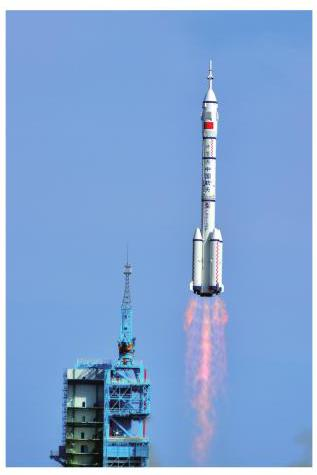
\includegraphics[max width=0.2\textwidth]{images/bo_d7fr3gc91nqc7381iccg_111_1144_418_317_475_0.jpg}
\end{center}
\hspace*{3em} 

这里 \(\ln\) 表示以 \(\mathrm{e}\) 为底的自然对数. 问当燃料质量至少是火箭质量的多少倍时,火箭的最大速度才能超过 \(8\mathrm{\;{km}}/\mathrm{s}\) . (结果精确到 0.1 倍)

解 根据题意, 得

\[
2\ln \left( {1 + \frac{M}{{m}_{0}}}\right)  > 8,
\]

\[
\ln \left( {1 + \frac{M}{{m}_{0}}}\right)  > 4,
\]

\[
1 + \frac{M}{{m}_{0}} > {\mathrm{e}}^{4},
\]

\[
\frac{M}{{m}_{0}} > {\mathrm{e}}^{4} - 1 \approx  {54.6} - 1 = {53.6}.
\]

所以，当燃料质量至少是火箭质量的 53.6 倍时，火箭的最大速度才能超过 \(8\mathrm{\;{km}}/\mathrm{s}\) .

例 8 现在我们可以回答必修课程 3.2 节一开始提出的问题: 在年利率为 5\%，且按年计复利的条件下，1 万元钱存多少年会超过5 万元?

解 问题是要找到一个最小的整数 \(n\) ,使得

\[
{\left( 1 + {0.05}\right) }^{n} > 5\text{ . }
\]

这等价于 \(n > {\log }_{1.05}5\) . 用计算器求精确到五位小数的常用对数值, 可得 \(\lg 5 \approx  {0.69897},\lg {1.05} \approx  {0.02119}\) . 由换底公式可得

\[
{\log }_{1.05}5 = \frac{\lg 5}{\lg {1.05}} \approx  \frac{0.69897}{0.02119} \approx  {32.98584}.
\]

所以，存 33 年会超过 5 万元.

最后, 从函数的角度看, 对数的换底公式说的是两个底数不同的对数函数实际上只相差一个常数倍. 事实上,设 \(a\text{ 、 }b\) 都是不等于 1 的正数,那么以 \(a\) 为底的对数函数 \(y = {\log }_{a}x\) 和以 \(b\) 为底的对数函数 \(y = {\log }_{b}x\) 仅相差一个常数倍,即

\[
{\log }_{b}x = \frac{1}{{\log }_{a}b}{\log }_{a}x,x > 0,
\]



\section*{}

\begin{center}
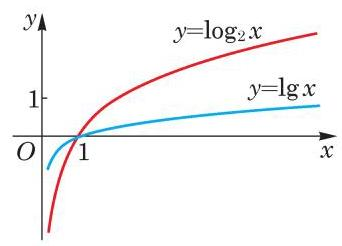
\includegraphics[max width=0.2\textwidth]{images/bo_d7fr3gc91nqc7381iccg_112_175_233_342_246_0.jpg}
\end{center}
\hspace*{3em} 

图 4-3-5

其中,因为 \({\log }_{a}b\) 不包含自变量 \(x\) ,在自变量 \(x\) 的变化过程中是不变的, 称为常量. 例如,

\[
\lg x = \frac{1}{{\log }_{2}{10}}{\log }_{2}x,
\]

函数 \(y = \lg x\) 和 \(y = {\log }_{2}x\) 的图像比较如图 4-3-5 所示.

\section*{练习 4.3(3)}

1. 动物死亡后,体内碳的放射同位素 \({}^{14}\mathrm{C}\) 的含量每年衰减 0.012\%,设在动物死亡的时刻 \(t = 0\) 时, \({}^{14}\mathrm{C}\) 的含量为 \(a\) .

(1)写出 \({}^{14}\mathrm{C}\) 的含量 \(y\) 随时间 \(t\) 变化的函数表达式；

(2)问至少经过多少年， \({}^{14}\mathrm{C}\) 的含量才能低于原来的 90\%.

2. 利用对数函数的单调性来估算对数 \({\log }_{2}5\) 的第一位小数的值.

\section*{习题 4.3}

\section*{A 组}

1. 求下列函数的定义域:

(1) \(y = {\log }_{a}\left( {x + {12}}\right)\) (常数 \(a > 0\) 且 \(a \neq  1\) )；

(2) \(y = {\log }_{2}\frac{1}{{x}^{2} - {2x} + 5}\) .

2. 已知对数函数 \(y = {\log }_{a}x\left( {a > 0\text{ 且 }a \neq  1}\right)\) 的图像经过点 \(\left( {3,2}\right)\) . 若点 \(P\left( {b,4}\right)\) 为此函数图像上的点,求实数 \(b\) 的值.

3. 在同一平面直角坐标系中画出下列函数的图像, 并指出这些函数图像之间的关系.

(1) \(y = {\log }_{3}x\) (2) \(y = {\log }_{\frac{1}{3}}x\) ；

(3) \(y = {\left( \frac{1}{3}\right) }^{x}\) .

4. 已知常数 \(a > 0\) 且 \(a \neq  1\) ，假设无论 \(a\) 取何值，函数 \(y = {\log }_{a}x - 1\) 的图像恒经过一个定点. 求此点的坐标.

5. 根据下列不等式,确定底数 \(a\) 的取值范围:

(1) \({\log }_{a}{0.2} < {\log }_{a}{0.1}\) ； (2) \({\log }_{a}\pi  > {\log }_{a}\mathrm{e}\) .

6. 已知 \(y = {\log }_{{a}^{2} - 1}x\) 在区间 \(\left( {0, + \infty }\right)\) 上是严格减函数，求实数 \(a\) 的取值范围.

7. 已知对数函数 \(y = {\log }_{a}x\left( {a > 1}\right)\) 在区间 \(\left\lbrack  {1,2}\right\rbrack\) 上的最大值比最小值大 1,求 \(a\) 的值.

\section*{}

B 组

1. 若 \(a > b > c > 1\) ,则下列不等式不成立的是\_\_\_\_\_. (填写所有不成立的不等式的序号)

 \circled{1}  \({\log }_{a}b > {\log }_{a}c\) ;  \circled{2}  \({\log }_{a}\frac{1}{b} > {\log }_{a}\frac{1}{c}\) ;  \circled{3}  \({\log }_{\frac{1}{a}}b > {\log }_{\frac{1}{a}}c\) ;  \circled{4}  \({\log }_{\frac{1}{a}}\frac{1}{b} > {\log }_{\frac{1}{a}}\frac{1}{c}\) .

2. 设常数 \(a > 0\) 且 \(a \neq  1\) ,求函数 \(y = {\log }_{a}\left( {a - {a}^{x}}\right)\) 的定义域.

3. 根据下列不等式,比较正数 \(m\) 及 \(n\) 的大小:

(1) \({\log }_{3}m < {\log }_{3}n\) ;

(2) \({\log }_{a}m < {\log }_{a}n\left( {a > 0\text{ 且 }a \neq  1}\right)\) ；

(3) \({\log }_{m}N < {\log }_{n}N\left( {0 < m < 1,0 < n < 1,0 < N < 1}\right)\) .

4. 设 \(0 < a < 1\) ,若 \({\log }_{a}\left( {4{x}^{2} - 1}\right)  < {\log }_{a}\left( {-2{x}^{2} + x + 1}\right)\) ,求实数 \(x\) 的取值范围.

5. 比较 \({22}^{23}\) 与 \({23}^{22}\) 的大小.

6. 如果 \({}^{237}\mathrm{U}\) 在不断的裂变中,每天所剩留质量与前一天剩留质量相比,按同一比例减少，且经过 7 天裂变，剩余的质量是原来的 50\%. 计算至少要经过多少天裂变，其剩留质量才小于原来的 10\%.

\section*{探究与实践}

\section*{幂函数、指数函数与对数函数增长速度的比较}

我们已经知道,如果指数函数的底数 \(a\) 大于 1,当自变量 \(x\) 增大时,指数函数 \(y = {a}^{x}\) 增长得非常快，称为“指数增长”. 类似地，可以分析底数 \(a\) 大于 1 的对数函数 \(y = {\log }_{a}x\) 的增长速度.

(1)计算函数 \(y = {0.01x}\) 和 \(y = \lg x\) 当 \(x = {10}^{2}\) ， \({10}^{4}\) ， \({10}^{6}\) ， \({10}^{8}\) ， \({10}^{10}\) 时的值，并由此比较两个函数的增长速度.

(2)计算函数 \(y = {x}^{0.1}\) 和 \(y = \lg x\) 当 \(x = {10}^{10}\) ， \({10}^{20}\) ， \({10}^{50}\) ， \({10}^{100}\) ， \({10}^{200}\) 时的值，并由此比较两个函数的增长速度.

(3)计算函数 \(y = {1.1}^{x}\) 和 \(y = \lg x\) 当 \(x = {10}^{2}\) ， \({10}^{4}\) ， \({10}^{6}\) ， \({10}^{8}\) ， \({10}^{10}\) 时的值，并由此比较两个函数的增长速度.

通过上述比较, 你对对数函数的增长速度有何体会?



\section*{课后阅读}

\section*{火箭速度的计算公式}

航天之父、俄罗斯科学家齐奥科夫斯基(K. E. Tsiolkovsky)于 1903 年给出火箭速度的计算公式

\[
v = {V}_{0}\ln \left( {1 + \frac{M}{{m}_{0}}}\right) .
\]

其中, \({V}_{0}\) 是燃料相对于火箭的喷射速度, \(M\) 是燃料的质量, \({m}_{0}\) 是火箭 (除去燃料) 的质量, \(v\) 是火箭将燃料喷射完之后达到的速度. 可以看出 \(v\) 与 \(M\) 是对数函数的关系,由于对数函数增长速度很慢,通过大量增加燃料 (即增加 \(\frac{M}{{m}_{0}}\) ) 难以达到航天器绕地球运行所需要的第一宇宙速度，据此他又提出了采用多级火箭发射航天器的设想.

现代运载火箭大多采用三级火箭，当第一级火箭的燃料用完时，点燃第二级火箭并抛弃第一级火箭,这相当于大大减小第二级火箭推进时的 \({m}_{0}\) ,从而在第二级火箭燃料用完时航天器可以达到较高的速度. 然后类似地点燃第三级火箭并抛弃第二级火箭, 最终可以将航天器送入太空轨道.

\section*{内容提要}

1. 幂函数 \(y = {x}^{a}\) 的定义域由指数 \(a\) 决定. 随着指数 \(a\) 的不同，幂函数的定义域是不同的.

2. 幂函数 \(y = {x}^{a}\) 有单调性:当 \(a > 0\) 时，它在区间 \(\left( {0, + \infty }\right)\) 上是严格增函数；而当 \(a < 0\) 时，它在区间 \(\left( {0, + \infty }\right)\) 上是严格减函数.

3. 指数函数 \(y = {a}^{x}\left( {a > 0\text{ 且 }a \neq  1}\right)\) 的定义域是全体实数.

4. 指数函数 \(y = {a}^{x}\left( {a > 0\text{ 且 }a \neq  1}\right)\) 有单调性:当 \(a > 1\) 时，它在 \(\mathbf{R}\) 上是严格增函数； 而当 \(0 < a < 1\) 时，它在 \(\mathbf{R}\) 上是严格减函数.

5. 对数函数 \(y = {\log }_{a}x\left( {a > 0\text{ 且 }a \neq  1}\right)\) 的定义域是全体正实数.

6. 对数函数 \(y = {\log }_{a}x\left( {a > 0\text{ 且 }a \neq  1}\right)\) 有单调性:当 \(a > 1\) 时，它在区间 \(\left( {0, + \infty }\right)\) 上是严格增函数；而当 \(0 < a < 1\) 时，它在区间 \(\left( {0, + \infty }\right)\) 上是严格减函数.

\section*{复习题}

\section*{A 组}

1. 填空题:

(1)若点 \(\left( {2,\sqrt{2}}\right)\) 在幂函数 \(y = {x}^{a}\) 的图像上，则该幂函数的表达式为\_\_\_\_\_； 若点 \(\left( {2,\sqrt{2}}\right)\) 在指数函数 \(y = {a}^{x}\) ( \(a > 0\) 且 \(a \neq  1\) )的图像上，则该指数函数的表达式为若点 \(\left( {\sqrt{2},2}\right)\) 在对数函数 \(y = {\log }_{a}x\left( {a > 0\text{ 且 }a \neq  1}\right)\) 的图像上，则该对数函数的表达式为\_\_\_\_\_.

(2)若幂函数 \(y = {x}^{k}\) 在区间 \(\left( {0, + \infty }\right)\) 上是严格减函数，则实数 \(k\) 的取值范围为\_\_\_\_\_.

(3)已知常数 \(a > 0\) 且 \(a \neq  1\) ，假设无论 \(a\) 为何值，函数 \(y = {a}^{x - 2} + 1\) 的图像恒经过一个定点. 则这个点的坐标为\_\_\_\_\_.

2. 选择题:

(1)若指数函数 \(y = {a}^{x}\left( {a > 0\text{ 且 }a \neq  1}\right)\) 在 \(\mathbf{R}\) 上是严格减函数，则下列不等式中，一定能成立的是 ( )

A. \(a > 1\) ; B. \(a < 0\) ;

C. \(a\left( {a - 1}\right)  < 0\) ; D. \(a\left( {a - 1}\right)  > 0\) .



(2)在同一平面直角坐标系中，一次函数 \(y = x + a\) 与对数函数 \(y = {\log }_{a}x\) ( \(a > 0\) 且 \(a \neq  1\) )的图像关系可能是 ( )

\begin{center}
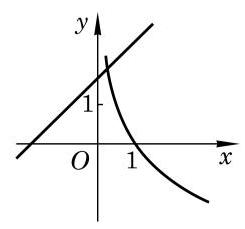
\includegraphics[max width=0.2\textwidth]{images/bo_d7fr3gc91nqc7381iccg_116_399_360_245_229_0.jpg}
\end{center}
\hspace*{3em} 

\begin{center}
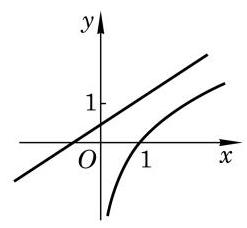
\includegraphics[max width=0.2\textwidth]{images/bo_d7fr3gc91nqc7381iccg_116_1026_361_247_228_0.jpg}
\end{center}
\hspace*{3em} 

A. B.

\begin{center}
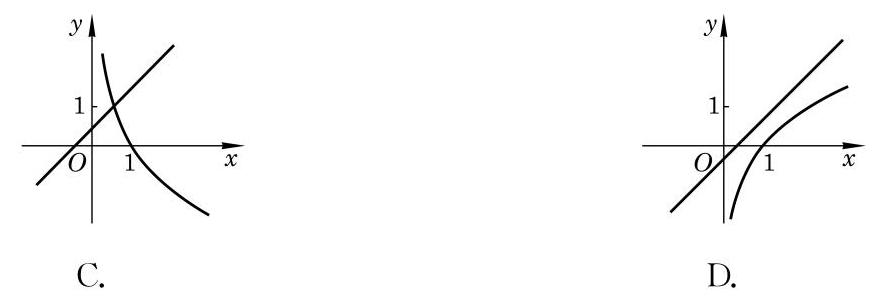
\includegraphics[max width=0.7\textwidth]{images/bo_d7fr3gc91nqc7381iccg_116_398_694_875_299_0.jpg}
\end{center}
\hspace*{3em} 

(第 2(2)题)

3. 求下列函数的定义域:

(1) \(y = {\left( x - 1\right) }^{\frac{5}{2}}\) ;

(2) \(y = {3}^{\sqrt{x - 1}}\) ；

(3) \(y = \lg \frac{1 + x}{1 - x}\) .

4. 比较下列各题中两个数的大小:

(1) \({0.1}^{0.7}\) 与 \({0.2}^{0.7}\) ；

(2) \({0.7}^{0.1}\) 与 \({0.7}^{0.2}\) ；

(3) \({\log }_{0.7}{0.1}\) 与 \({\log }_{0.7}{0.2}\) .

5. 设点 \(\left( {\sqrt{2},2}\right)\) 在幂函数 \({y}_{1} = {x}^{a}\) 的图像上,点 \(\left( {-2,\frac{1}{4}}\right)\) 在幂函数 \({y}_{2} = {x}^{b}\) 的图像上. 当 \(x\) 取何值时, \({y}_{1} = {y}_{2}\) ?

6. 设 \(a = {\left( \frac{2}{3}\right) }^{x},b = {x}^{\frac{3}{2}}\) 及 \(c = {\log }_{\frac{2}{3}}x\) ,当 \(x > 1\) 时,试比较 \(a\text{ 、 }b\) 及 \(c\) 之间的大小关系.

7. 设常数 \(a > 0\) 且 \(a \neq  1\) ,若函数 \(y = {\log }_{a}\left( {x + 1}\right)\) 在区间 \(\left\lbrack  {0,1}\right\rbrack\) 上的最大值为 1,最小值为 0,求实数 \(a\) 的值.

8. 如果光线每通过一块玻璃其强度要减少 \({10}\%\) ,那么至少需要将多少块这样的玻璃重叠起来,才能使通过它们的光线强度低于原来的 \(\frac{1}{3}\) ?





B 组

1. 填空题:

(1)已知 \(m \in  \mathbf{Z}\) ,设幂函数 \(y = {x}^{{m}^{2} - {4m}}\) 的图像关于原点成中心对称,且与 \(x\) 轴及 \(y\) 轴均无交点,则 \(m\) 的值为\_\_\_\_\_.

(2)设 \(a\) 、 \(b\) 为常数，若 \(0 < a < 1\) ， \(b <  - 1\) ，则函数 \(y = {a}^{x} + b\) 的图像必定不经过第象限.

2. 选择题:

(1)若 \(m > n > 1\) ，而 \(0 < x < 1\) ，则下列不等式正确的是 ( )

A. \({m}^{x} < {n}^{x}\) ; B. \({x}^{m} < {x}^{n}\) ;

C. \({\log }_{x}m > {\log }_{x}n\) ; D. \({\log }_{m}x < {\log }_{n}x\) .

( 2 )在同一平面直角坐标系中，二次函数 \(y = a{x}^{2} + {bx}\) 与指数函数 \(y = {\left( \frac{b}{a}\right) }^{x}\) 的图像关系可能为 ( )

\begin{center}
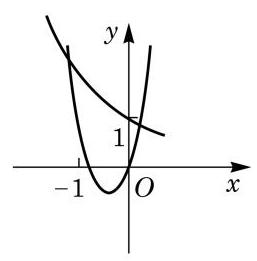
\includegraphics[max width=0.2\textwidth]{images/bo_d7fr3gc91nqc7381iccg_117_364_1020_257_261_0.jpg}
\end{center}
\hspace*{3em} 

\begin{center}
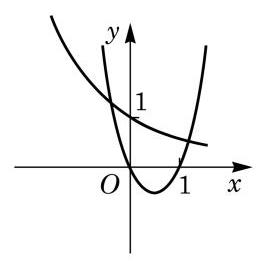
\includegraphics[max width=0.2\textwidth]{images/bo_d7fr3gc91nqc7381iccg_117_992_1020_259_261_0.jpg}
\end{center}
\hspace*{3em} 

A. B.

\begin{center}
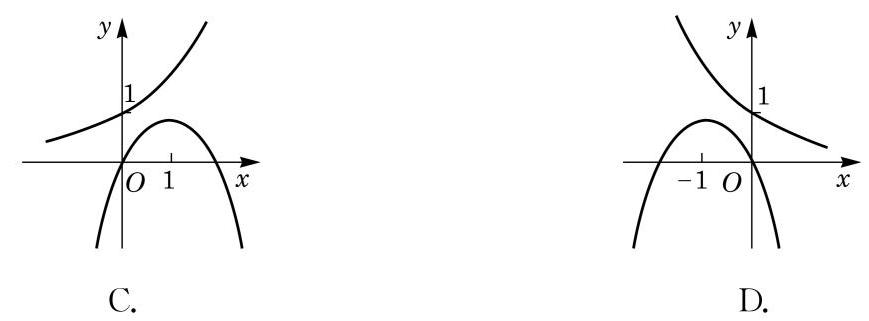
\includegraphics[max width=0.7\textwidth]{images/bo_d7fr3gc91nqc7381iccg_117_369_1384_869_321_0.jpg}
\end{center}
\hspace*{3em} 

(第 2(2)题)

3. 设 \(a\) 为常数且 \(0 < a < 1\) ,若 \(y = {\left( {\log }_{a}\frac{3}{5}\right) }^{x}\) 在 \(\mathbf{R}\) 上是严格增函数,求实数 \(a\) 的取值范围.

4. 在同一平面直角坐标系中,作出函数 \(y = {\left( \frac{1}{2}\right) }^{x}\) 及 \(y = {x}^{\frac{1}{2}}\) 的大致图像,并求方程 \({\left( \frac{1}{2}\right) }^{x} = {x}^{\frac{1}{2}}\) 的解的个数.

5. 已知集合 \(A = \left\{  {y\left| {\;y = {\left( \frac{1}{2}\right) }^{x}}\right. ,x \in  \lbrack  - 2,0)}\right\}\) ，用列举法表示集合 \(B = \left\{  {y \mid  y = {\log }_{3}x}\right.\) ， \(x \in  A\) 且 \(y \in  \mathbf{Z}\}\) .

\section*{拓展与思考}

1. \({\log }_{2}3\) 是有理数吗? 请证明你的结论.

2. 仅利用对数函数的单调性和计算器上的乘方功能来确定对数 \({\log }_{2}3\) 第二位小数的值.

\section*{第 5 章 函数的概念、 性质及应用}

在初中和上一章中，我们已学习了一次函数、二次函数、反比例函数、幂函数、指数函数及对数函数. 这些函数的共同点是有两个变量, 当其中的一个变量在某个范围内变化时, 另一个变量就按照某种规则随之变化. 这种一个变量随着另一个变量的变化而变化的对应关系, 在数学上就称为函数. 在对二次函数、幂函数、指数函数与对数函数的研究中, 已经可以看到不同的函数间有一些共同的性质, 本章将概括有关函数的一些比较重要的性质, 并用严格的数学语言加以描述.

函数是刻画世间万物之间联系的有力工具，借助于函数, 可以更好地掌握事物的发展规律, 从而深化人们的认识. 函数概念的引入, 使数学本身也经历了从常量到变量、 从有限到无限的发展, 从而逐步由初等数学走向高等数学. 学好函数, 对进一步学习以后的一些数学知识, 如三角、 微积分等，都是非常必要的.

\section*{}

\section*{5.1 函数}

1 函数

我们已经学习了正比例函数、反比例函数、一次函数、二次函数、幂函数、指数函数及对数函数等.

例如,对于正比例函数 \(y = {2x}\) ,变量 \(x\) 的取值范围是 \(\mathbf{R}\) ,其对应关系是将一个实数对应到它的 2 倍. 当变量 \(x = 1\) 时,对应得到唯一的值 \(y = 2 \times  1 = 2\) ; 当变量 \(x =  - 3\) 时,对应得到唯一的值 \(y = 2 \times  \left( {-3}\right)  =  - 6\) ; 当变量 \(x\) 取遍一切实数时,对应得到所有的实数 \(y\) .

又如,对于对数函数 \(y = {\log }_{3}x\) ,变量 \(x\) 的取值范围是 \(\left( {0, + \infty }\right)\) . 其对应关系是将 \(\left( {0, + \infty }\right)\) 中的实数对应到它的以 3 为底的对数. 当变量 \(x = \frac{1}{3}\) 时,对应得到唯一的值 \(y =  - 1\) ; 当变量 \(x = 1\) 时, 对应得到唯一的值 \(y = 0\) ; 当变量 \(x\) 取遍一切正数时,对应得到所有的实数 \(y\) .

在这些例子中, 都出现了两个处于变化之中的量, 其中一个量之值随另一个量之值的确定而按一定的对应关系唯一确定, 从而随着另一个量在一定范围内的变化而相应地发生变化. 在用数学工具解决实际问题的过程中, 我们还会遇到其他一些类似的情况. 由此可抽象出函数的概念.

定义 设 \(D\) 是一个非空的实数集,如果按照某种确定的对应关系 \(f\) ,使对集合 \(D\) 中的任意给定的 \(x\) ,都有唯一的实数 \(y\) 与之对应,就称这个对应关系 \(f\) 为集合 \(D\) 上的一个函数 (function), 记作

\[
y = f\left( x\right) ,x \in  D.
\]

其中, \(x\) 叫做自变量 (independent variable),其取值范围 (数集 D)称为该函数的定义域(domain).



\HRule

对应关系常用小写字母，如 \(f\text{ 、 }g\text{ 、 }h\) 等表示.

\HRule



此时,就称 \(y\) 是 \(x\) 的函数. 当自变量 \(x\) 取值 \({x}_{0}\) 时,由对应关系 \(f\) 所确定的对应于 \({x}_{0}\) 的值 \({y}_{0}\) ,称为函数在 \({x}_{0}\) 处的函数值, 记作 \({y}_{0} = f\left( {x}_{0}\right)\) .

所有函数值组成的集合 \(\{ y \mid  y = f\left( x\right) ,x \in  D\}\) 称为这个函数的值域(range).

根据函数的定义, 在定义域和对应关系确定的时候, 这个函数就完全被确定了, 从而值域也随之被确定. 因此, 定义域和对应关系称为函数的两个要素.

在之前学习具体的函数, 如幂函数、指数函数及对数函数的时候，我们往往只写出反映函数对应关系的表达式，如 \(y = {x}^{\frac{1}{2}},y = {2}^{x},y = {\log }_{3}x\) 等,而不明显地写出其定义域. 此时,函数 \(y = f\left( x\right)\) 的定义域由使得其表达式 \(f\left( x\right)\) 有意义的全体实数组成.

例 1 求下列函数的定义域:

(1) \(y = \frac{1}{{x}^{2} - 1}\) ;

(2) \(y = {\log }_{2}\left( {x + 1}\right)\) ；

(3) \(y = \frac{\sqrt{x + 3}}{x - 1}\) .

解 (1) 定义域 \(D = \left\{  {x \mid  {x}^{2} - 1 \neq  0}\right\}   = \{ x \mid  x \neq   \pm  1\}\) .

(2)定义域 \(D = \{ x \mid  x + 1 > 0\}  = \left( {-1, + \infty }\right)\) .

(3)解不等式组

\[
\left\{  \begin{array}{l} x + 3 \geq  0, \\  x - 1 \neq  0, \end{array}\right.
\]

得

\[
x \geq   - 3\text{ 且 }x \neq  1\text{ . }
\]

故定义域 \(D = \lbrack  - 3,1) \cup  \left( {1, + \infty }\right)\) .

在实际问题中, 有关函数的定义域应该受到问题实际意义的制约. 例如,某物体作自由落体运动时,其位移 \(s\) 关于时间 \(t\) 的函数可表示为 \(s = \frac{1}{2}g{t}^{2}\) ,其中的自变量 \(t\) 就受到 \(0 \leq  t \leq  T\) 的限制 ( \(g\) 是重力加速度，而 \(T\) 表示下落的总时间).

除定义域外, 函数的另一要素是对应关系.

如果两个函数的定义域和对应关系都完全一致, 就称这两个函数是相同的.





这样, \(y = {x}^{2}\) 与 \(y = {x}^{2},x \in  \left\lbrack  {-1,1}\right\rbrack\) 是两个不同的函数.

此外,同一个对应关系可能有不同的表述形式. 例如, \(y = x\) 与 \(y = {\left( \sqrt[3]{x}\right) }^{3}\) 实际上是相同的.

例 2 判断下列函数与函数 \(y = x\) 是否相同,并说明理由:

(1) \(y = {\left( \sqrt{x}\right) }^{2}\) ; (2) \(y = \ln {\mathrm{e}}^{x}\) ；

(3) \(y = \frac{{x}^{2}}{x}\) ； (4) \(y = \sqrt[4]{{x}^{4}}\) .

解 (1) 负数不属于 \(y = {\left( \sqrt{x}\right) }^{2}\) 的定义域,因此该函数的定义域与 \(y = x\) 的定义域不同,它与 \(y = x\) 不是相同的函数.

?

\HRule

你能再举出几组对应关系一致、但表述形式不同的两个相同的函数吗?

\HRule

(2) \(y = \ln {\mathrm{e}}^{x} = x\ln \mathrm{e} = x\) 的定义域为 \(\mathbf{R}\) ,并且其对应关系是将任一给定的实数 \({x}_{0}\) 对应到 \({x}_{0}\) ,与 \(y = x\) 的对应关系一致,因此该函数与 \(y = x\) 是相同的函数.

(3)0 不在 \(y = \frac{{x}^{2}}{x}\) 的定义域中，因此该函数的定义域与 \(y = x\) 的定义域不同,从而与 \(y = x\) 不是相同的函数.

(4) \(y = \sqrt[4]{{x}^{4}}\) 的对应关系将 -1 对应到了 1，而不是 -1 ，它与 \(y = x\) 的对应关系不同,因此该函数与 \(y = x\) 不是相同的函数.

在例 2 中,只有 \(y = \ln {\mathrm{e}}^{x}\) 的对应关系和定义域与 \(y = x\) 的相同, 它们是相同的函数.

根据已经学过的一些简单函数的值域, 可以求得稍复杂函数的值域.

例 3 求函数 \(y = \frac{1}{{2}^{x} + 1}\) 的值域.

解 该函数的定义域为 \(\mathbf{R}\) .

根据指数函数的性质,当 \(x\) 取遍所有实数时, \({2}^{x}\) 的取值范围为 \(\left( {0, + \infty }\right)\) ,因而 \({2}^{x} + 1\) 的取值范围为 \(\left( {1, + \infty }\right)\) .

又根据不等式的性质,令 \(t = {2}^{x} + 1\) ,当 \(t\) 取遍 \(\left( {1, + \infty }\right)\) 中所有数时, \(\frac{1}{t}\) 的取值范围为 \(\left( {0,1}\right)\) .

因此,函数 \(y = \frac{1}{{2}^{x} + 1}\) 的值域为 \(\left( {0,1}\right)\) .

\section*{练习 5.1(1)}

1. 求下列函数的定义域:

(1) \(y = \sqrt{\left( {x - 2}\right) \left( {x + 3}\right) }\) ;

\section*{}

(2) \(y = \frac{1}{1 - \sqrt{x - 1}}\) .

2. 下列四组函数中, 同组的两个函数是相同函数的是 ( )

A. \(y = \left| x\right|\) 与 \(y = {\left( \sqrt{x}\right) }^{2}\) ; B. \(y = x\) 与 \(y = {\mathrm{e}}^{\ln x}\) ;

C. \(y = x\) 与 \(y = \sqrt[5]{{x}^{5}}\) ; D. \(y = x\) 与 \(y = {\left( \frac{1}{x}\right) }^{-1}\) .

3. 求下列函数的值域:

(1) \(y = {\left( \lg x\right) }^{2} + 1,x \in  \left( {0, + \infty }\right)\) ; (2) \(y = 3{x}^{2} - {4x} + 1,x \in  \left\lbrack  {0,1}\right\rbrack  .\)

\section*{2 函数的表示方法}

用一个数学表达式来表示两个变量之间的对应关系, 这种表示函数的方法称为解析法.

例如, \(y = {3x} + 2,y = {x}^{2} + {2x} + 1,y = \sqrt{{x}^{2} + 1} \; \left( {x \in  \left\lbrack  {0,1}\right\rbrack  }\right) ,y = {\log }_{2}\left( {{2}^{x} - 1}\right)\) 等都是用解析法表示的函数. 作自由落体运动的物体的位移 \(s\) 与时间 \(t\) 满足 \(s = \frac{1}{2}g{t}^{2},t \in  \left\lbrack  {0,T}\right\rbrack\) ( \(g\) 是重力加速度),也是用解析法来表示的函数.

通过列出自变量的值与对应函数值的相应表格来表达函数关系的方法称为列表法, 列表法通常用在定义域为有限集的情况.

例如, 表 5-1 列出了《中国统计年鉴一2019》发布的 2000 年至 2016 年的国内生产总值 (GDP).

表 5-1 2000 年至 2016 年中国 GDP 变化表

\begin{center}
\adjustbox{max width=\textwidth}{
\begin{tabular}{|c|c|c|c|}
\hline
年份 & GDP/亿元 & 年份 & GDP/亿元 \\
\cline{1-4}
2000 & 100 280 & 2009 & 348 518 \\
\cline{1-4}
2001 & 110 863 & 2010 & 412 119 \\
\cline{1-4}
2002 & 121 717 & 2011 & 487 940 \\
\cline{1-4}
2003 & 137 422 & 2012 & 538580 \\
\cline{1-4}
2004 & 161 840 & 2013 & 592963 \\
\cline{1-4}
2005 & 187319 & 2014 & 641 281 \\
\cline{1-4}
2006 & 219439 & 2015 & 685 993 \\
\cline{1-4}
2007 & 270092 & 2016 & 740061 \\
\cline{1-4}
2008 & 319 245 & \phantom{X} & \phantom{X} \\
\cline{1-4}
\hline
\end{tabular}
}
\end{center}

注:未包括中国香港、澳门特别行政区和台湾省的地区生产总值数据.





从表 5-1 中可以看出, 当自变量年份 (2000 至 2016 中的整数)确定时，可按照表中所给出的对应关系，查到该年度我国的 GDP 值作为函数值. 该函数的定义域为 \(\{ {2000},{2001},{2002},\cdots\) , 2016),是一个有限集.

我们知道,对于函数 \(y = f\left( x\right) ,x \in  D\) ,其定义域 \(D\) 中每一个 \(x\) 的值都有唯一的一个 \(y\) 值与之对应. 把这两个对应的数构成的有序实数对 \(\left( {x,y}\right)\) 作为点 \(P\) 的坐标,记作 \(P\left( {x,y}\right)\) . 所有这些点组成的集合 \(G\) 叫做函数 \(y = f\left( x\right) ,x \in  D\) 的图像 (graph), 即

\[
G = \{ \left( {x,y}\right)  \mid  y = f\left( x\right) ,x \in  D\} .
\]

可以看出,如果对定义域 \(D\) 中的实数 \({x}_{0}\) ,有 \(f\left( {x}_{0}\right)  = {y}_{0}\) , 那么点 \(P\left( {{x}_{0},{y}_{0}}\right)\) 一定在该函数的图像上; 反之,如果点 \(P\left( {{x}_{0},{y}_{0}}\right)\) 在该函数的图像上,那么必有 \({x}_{0} \in  D\) ,且 \({y}_{0} = f\left( {x}_{0}\right)\) .

常见的一次函数、二次函数、幂函数、指数函数及对数函数的图像, 已经在初中和上一章中学过了.

例 4 作出函数 \(y = \frac{x}{{x}^{2} + 1}\) 的大致图像.

解 取自变量 \(x\) 的值分别为 \(- 3\text{ 、 } - \frac{5}{2}\text{ 、 } - 2\text{ 、 } - \frac{3}{2}\text{ 、 } - 1\) 、 \(- \frac{1}{2}\text{ 、 }0\text{ 、 }\frac{1}{2}\text{ 、 }1\text{ 、 }\frac{3}{2}\text{ 、 }2\text{ 、 }\frac{5}{2}\text{ 、 }3\) ,计算出相应的函数值. 在平面直角坐标系中标出相应的点, 并用光滑的曲线连接这些点, 得大致图像如图 5-1-1 所示.

\begin{center}
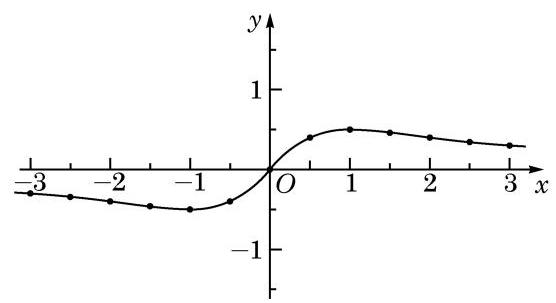
\includegraphics[max width=0.4\textwidth]{images/bo_d7fr3gc91nqc7381iccg_124_744_1653_556_303_0.jpg}
\end{center}
\hspace*{3em} 

图 5-1-1

利用函数的图像来表示函数的方法称为图像法.

\HRule

该函数的图像会出现在第二或第四象限吗? 为什么?

需要注意的是， 绘制在纸上的或计算机屏幕上的函数图像, 终究只是大致的图像, 它们无法精确地表示一个函数. 但大致的图像能够帮助我们直观地了解函数的性质, 从而能更好地发现和研究有关函数的性质. “数形结合”的方法是研究函数的重要方法之一。

\HRule

例 5 以下图形中, 哪些是函数的图像, 哪些不是?

\begin{center}
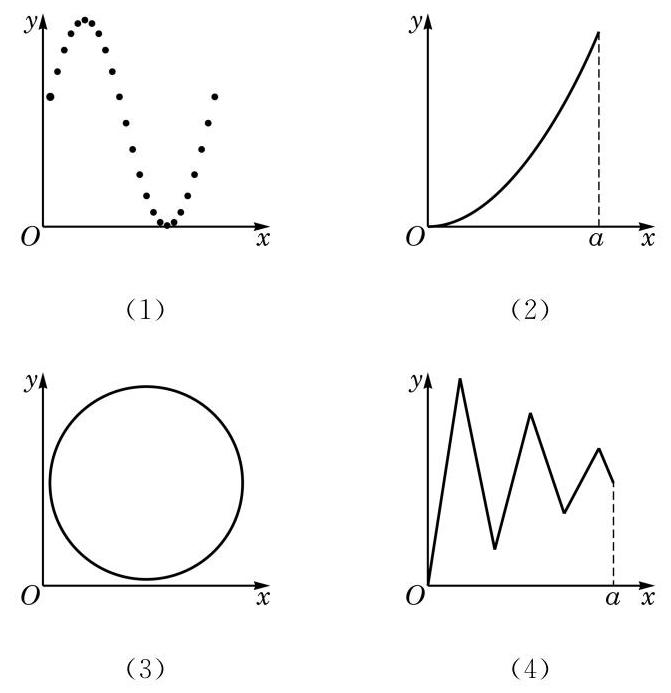
\includegraphics[max width=0.5\textwidth]{images/bo_d7fr3gc91nqc7381iccg_125_290_314_671_693_0.jpg}
\end{center}
\hspace*{3em} 

图 5-1-2

解(1)这是函数的图像. 该函数的定义域是由有限个数构成的集合，定义域中每个自变量的值对应的函数值唯一确定.

(2)这是函数的图像. 该函数的定义域是区间 \(\left\lbrack  {0,a}\right\rbrack\) ，定义域中的每个自变量的值所对应的函数值唯一确定.

(3)这不是函数的图像. 如图 5-1-3， \({x}_{0}\) 对应了 \({y}_{1}\) 和 \({y}_{2}\) .

\begin{center}
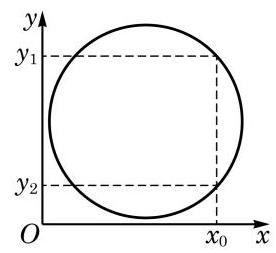
\includegraphics[max width=0.2\textwidth]{images/bo_d7fr3gc91nqc7381iccg_125_485_1495_276_253_0.jpg}
\end{center}
\hspace*{3em} 

图 5-1-3

(4)这是函数的图像. 该函数的定义域是区间 \(\left\lbrack  {0,a}\right\rbrack\) ,定义域中的每个自变量的值所对应的函数值唯一确定.

前文中 2000 年至 2016 年中国国内生产总值 (GDP) 关于年份的函数，也可以用图像法表示，如图 5-1-4 所示.

\HRule

在检验平面直角坐标系中的一个图形是否为函数的图像时, 需要注意该图形反映的对应关系是否符合函数的定义, 即定义域中的每一个 \(x\) 的值是否对应到唯一的一个 \(y\) 的值.

\HRule

\begin{center}
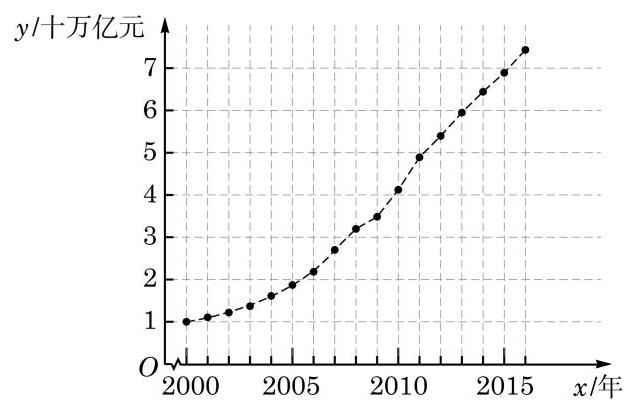
\includegraphics[max width=0.5\textwidth]{images/bo_d7fr3gc91nqc7381iccg_126_706_257_628_407_0.jpg}
\end{center}
\hspace*{3em} 

图 5-1-4

函数图像上所有点的横坐标的集合就是该函数的定义域, 而纵坐标的集合就是该函数的值域.

\HRule

分段表示法也是一种解析法. 用分段表示法表示一个函数时, 其定义域就是每一部分中自变量的取值范围的并集.

\HRule

在用解析法表示函数时, 有一些函数在不同的区间上可以有不同的表达式. 例如,函数 \(y = \left| x\right|\) 就是通过

\[
y = \left\{  \begin{array}{ll} x, & x \geq  0, \\   - x, & x < 0 \end{array}\right.
\]

来定义的. 这样表示函数的方法叫做分段表示法.

例 6 某车辆装配车间每 2 h 装配完成一辆车. 按照计划, 该车间今天生产 8 h. 用解析法和图像法分别表示从当天开始生产的时刻起所经过的时间 \(x\) (单位: \(\mathrm{h}\) )与装配完成的车辆数 \(y\) (单位: 辆)之间的函数 \(y = f\left( x\right)\) .

解 由题意,当 \(x \in  \lbrack 0,2)\) 时, \(y = 0\) ; 当 \(x \in  \lbrack 2,4)\) 时, \(y = 1\) ; 当 \(x \in  \lbrack 4,6)\) 时, \(y = 2\) ; 当 \(x \in  \lbrack 6,8)\) 时, \(y = 3\) ; 当 \(x = 8\) 时, \(y = 4\) .

\[
y = \left\{  \begin{array}{ll} 0, & 0 \leq  x < 2, \\  1, & 2 \leq  x < 4, \\  2, & 4 \leq  x < 6, \\  3, & 6 \leq  x < 8, \\  4, & x = 8. \end{array}\right.
\]

\begin{center}
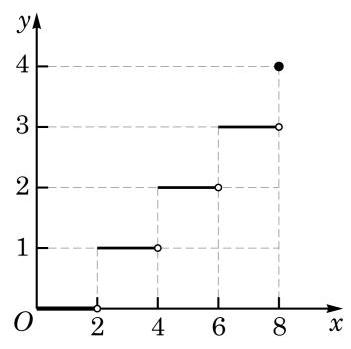
\includegraphics[max width=0.3\textwidth]{images/bo_d7fr3gc91nqc7381iccg_126_176_1543_351_349_0.jpg}
\end{center}
\hspace*{3em} 

图 5-1-5

可以用如下的分段表示法表示 \(y\) 与 \(x\) 之间的函数关系:

该函数的大致图像如图 5-1-5 所示.

Q

\HRule

不大于 \(x\) 的最大整数,称为实数 \(x\) 的整数部分.

\HRule

数学上,常用 \(\left\lbrack  x\right\rbrack\) 表示不大于 \(x\) 的最大整数. 注意到当 \({2k} \leq  x < {2k} + 2\left( {k \in  \mathbf{Z}}\right)\) 时, \(k \leq  \frac{x}{2} < k + 1\) ,从而 \(\left\lbrack  \frac{x}{2}\right\rbrack   = k\) . 使用此





符号,例 6 中的函数可以简洁地表示为 \(y = \left\lbrack  \frac{x}{2}\right\rbrack  ,x \in  \left\lbrack  {0,8}\right\rbrack\) .

\section*{练习 5.1(2)}

1. 作下列函数的大致图像:

(1) \(y =  - \left| x\right|\) ； (2) \(y = \sqrt{x + 2}\) ；

(3) \(y = \frac{1}{{x}^{2} + 1}\) ； (4) \(y = \frac{{2x} - 1}{x - 1}\) .

2. 根据下图的函数图像,用解析法表示 \(y\) 关于 \(x\) 的函数.

\begin{center}
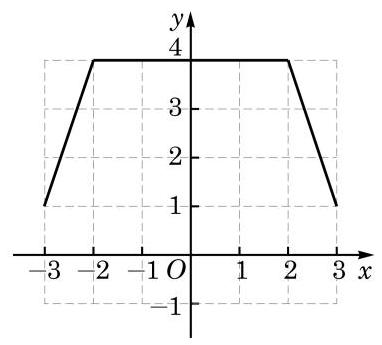
\includegraphics[max width=0.3\textwidth]{images/bo_d7fr3gc91nqc7381iccg_127_617_742_382_345_0.jpg}
\end{center}
\hspace*{3em} 

(第 2 题)

\section*{习题 5.1}

\section*{A 组}

1. 求下列函数的定义域:

(1) \(y = \frac{1}{{x}^{2} + {2x} - 3}\) ；

(2) \(y = \sqrt{4 - {3x} - {x}^{2}}\) ；

(3) \(y = \sqrt{x - 2} + \sqrt{x + 3}\) ；

(4) \(y = \frac{1}{\lg \left( {x + 2}\right) } + \frac{1}{\sqrt{5 - x}}.\)

2. 设 \(p\text{ 、 }q\) 是常数,函数 \(y = f\left( x\right)\) 的表达式为 \(f\left( x\right)  = {x}^{2} + {px} + q\) . 若 \(f\left( 1\right)  = f\left( 2\right)  = 0\) , 求 \(f\left( {-1}\right)\) .

3. 观察下列函数的图像, 并写出它们的值域:



\begin{center}
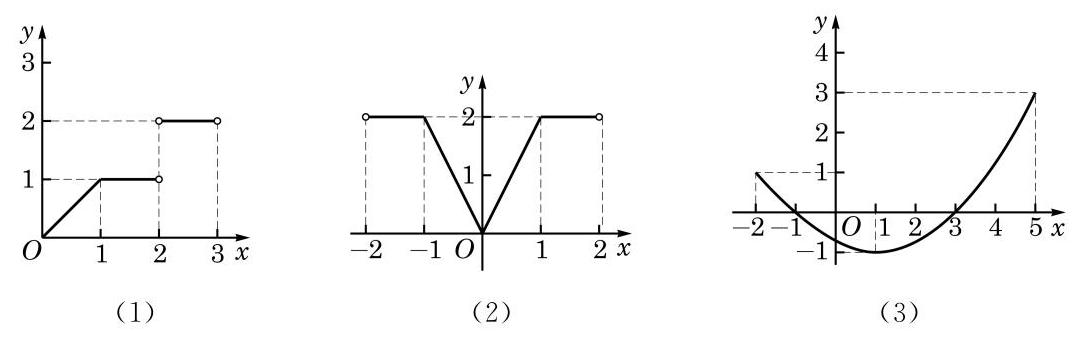
\includegraphics[max width=0.9\textwidth]{images/bo_d7fr3gc91nqc7381iccg_128_299_231_1079_338_0.jpg}
\end{center}
\hspace*{3em} 

(第 3 题)

\section*{B 组}

1. 设 \(a\) 是常数，求下列函数的定义域:

(1) \(y = \frac{1}{\left| x\right|  - a}\) ; (2) \(y = \sqrt{x\left( {x - a}\right) }\) .

2. 已知函数 \(y = f\left( x\right)\) 的表达式为 \(f\left( x\right)  = \left\{  \begin{array}{ll} {2x}\left( {3 + x}\right) , & x \geq  0, \\  {2x}\left( {3 - x}\right) , & x < 0. \end{array}\right.\) 求 \(f\left( 2\right) ,f\left( {-4}\right)\) 及 \(f\left( {-a}\right)\) ,其中 \(a\) 为实数.

\section*{课后阅读}

\section*{函数概念的形成和发展}

17 世纪是工业生产和科学技术飞速发展的时代，在对天文和航海技术的探索中，科学家们往往需要研究一些运动中的对象, 如天体位置、航海中经纬度等. 这些问题的实质都是分析研究两个变化中的量之间的关系, 并据此描述物体的变化规律. 这是函数概念产生和发展的背景.

在 17 世纪早期, 意大利科学家伽利略(G. Galilei)、法国数学家笛卡儿(R. Descartes)等已经注意到了一个变量对另一个变量的依赖关系, 但并没有提炼出函数的概念. 17 世纪后期, 英国数学家牛顿(I. Newton)和德国数学家莱布尼茨(G. W. Leibniz)在分别创立微积分时, 考虑的主要对象还是曲线, 而牛顿则一直用“流量”一词来表示变量之间的关系.

“函数”(function)一词作为数学概念首先由莱布尼茨引入，用于描述随曲线变化而变化的几何量, 如坐标、切线等. 此后, 瑞士数学家约翰·伯努利 (John Bernoulli) 首次给出了明确的函数定义，他将函数描述为 “由变量和常量以某种方式组成的量”. 将函数作为中心概念进行数学研究并作为微积分基础的是瑞士数学家欧拉 (L. Euler). 欧拉称变量的函数是一个解析表达式,引入了函数符号 \(f\left( x\right)\) 并沿用至今. 欧拉还将函数分成代数函数 (由



\section*{}

四则运算和开根等运算组成的函数)和超越函数 (含指数、对数、三角运算等的函数), 他也是第一个将正弦、余弦等当作函数处理的数学家. 欧拉的很多数学发现基于他的函数观点. 在 1755 年, 欧拉将函数的定义修改为: 如果某些变量以某种方式依赖于另一些变量, 即当后面的变量变化时, 前面的变量也随之变化, 那么称前面的变量是后面变量的函数.

在欧拉时代, 人们还是习惯于用表达式来表示函数. 随着对微积分研究的深入, 18 世纪末 19 世纪初，人们对函数的认识有了进一步提高. 德国数学家狄利克雷(P. G. L. Dirichlet) 于 1837 年提出了如下的函数的定义: 若对于 \(x\) 的每一个值, \(y\) 总有一个唯一确定的值与之对应,则称 \(y\) 是 \(x\) 的函数. 这个定义较清楚地说明了函数概念的本质是对应关系, 这个对应关系可以用公式、图像、表格或其他形式表示. 这个概念非常清晰, 很快被数学家所接受. 到 19 世纪 70 年代以后，随着集合论的出现，就有了使用规范的集合语言表述的函数定义, 函数概念也就更加精确了.

中文“函数”一词是由我国清代数学家李善兰在 1859 年和英国人伟烈亚力(A. Wylie) 合译《代微积拾级》时从英文“function”翻译而来，这一名词一直使用至今.

从上面介绍可以看出, 历史上函数概念的建立是从模糊到清晰、从朴素到深入逐步完善的, 这符合人们认识事物的一般规律. 了解函数概念的发展历史, 对于我们更好地理解函数这一重要的数学概念会有很大的帮助.

\section*{5.2 函数的基本性质}

函数是描述客观世界中变量关系和规律的最为基本的数学语言和工具. 了解了函数, 就把握了相应事物的变化规律. 为了深入了解函数，有必要研究其有关的性质，因此，学习函数的性质非常重要.

函数的性质是多种多样的, 且不同的函数有不同的性质.

关于一次函数、二次函数、幂函数、指数函数和对数函数, 我们已经接触过很多研究其性质的方法, 且已经知道了不少结论. 本节将以此为出发点, 概括函数的一些常见的性质.

\section*{3 函数的奇偶性}

在生活中，我们经常遇到对称的图形. 拱桥的桥面形成的弧, 就可以视为是轴对称的. 如果把桥面抽象成一条曲线, 以曲线的最高点为原点,过原点作一水平直线为 \(x\) 轴,再过原点作一竖直直线为 \(y\) 轴,那么这条由拱桥桥面抽象出的曲线就成为一个函数的图像, 并且该图像的一个特点是关于 \(y\) 轴成轴对称,如图 5-2-1 所示.

\begin{center}
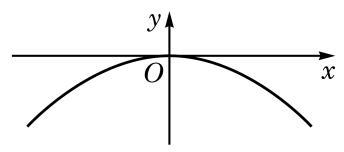
\includegraphics[max width=0.2\textwidth]{images/bo_d7fr3gc91nqc7381iccg_130_176_1208_344_152_0.jpg}
\end{center}
\hspace*{3em} 

图 5-2-1

在学习二次函数和幂函数时,我们知道,形如 \(y = a{x}^{2} + c \; \left( {a \neq  0}\right)\) 的二次函数和幂函数 \(y = {x}^{-\frac{2}{3}}\) 的图像都是关于 \(y\) 轴成轴对称的, 如图 5-2-2 所示.

\begin{center}
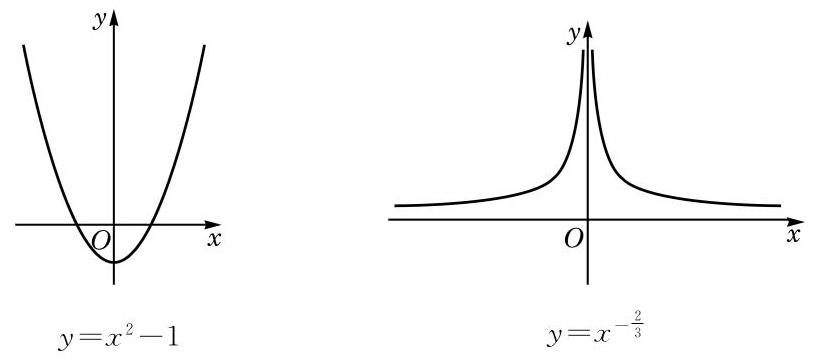
\includegraphics[max width=0.6\textwidth]{images/bo_d7fr3gc91nqc7381iccg_130_615_1675_813_360_0.jpg}
\end{center}
\hspace*{3em} 

图 5-2-2

?

\HRule

图 5-2-2 中的这两个函数的图像都具有关于 \(y\) 轴成轴对称的共同特征, 其相应的自变量与函数值的对应关系是如何体现这个特征的?

\HRule

一个图形关于某条直线 \(l\) 成轴对称,是指该图形上的任意一

点关于直线 \(l\) 的对称点也在此图形上.

现在，我们来探究 “函数的图像关于 \(y\) 轴成轴对称” 这一条件的等价表达形式.

在函数 \(y = f\left( x\right) ,x \in  D\) 的图像 \(G\) 上任取一点 \(P\left( {{x}_{1},{y}_{1}}\right)\) ,就有

\[
{x}_{1} \in  D\text{ ,并且 }{y}_{1} = f\left( {x}_{1}\right) \text{ . }
\]

\begin{center}
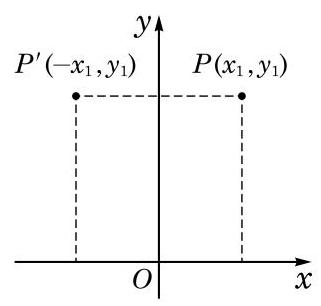
\includegraphics[max width=0.2\textwidth]{images/bo_d7fr3gc91nqc7381iccg_131_1138_530_321_306_0.jpg}
\end{center}
\hspace*{3em} 

图 5-2-3

点 \(P\left( {{x}_{1},{y}_{1}}\right)\) 关于 \(y\) 轴的对称点为 \({P}^{\prime }\left( {-{x}_{1},{y}_{1}}\right)\) (图 5-2-3). 如果函数 \(y = f\left( x\right) ,x \in  D\) 的图像关于 \(y\) 轴成轴对称,那么 \({P}^{\prime }\left( {-{x}_{1},{y}_{1}}\right)\) 也在图像 \(G\) 上,即

\[
- {x}_{1} \in  D\text{ ,并且 }{y}_{1} = f\left( {-{x}_{1}}\right) \text{ . }
\]

这说明,如果函数 \(y = f\left( x\right) ,x \in  D\) 的图像关于 \(y\) 轴成轴对称,那么对于任意给定的 \(x \in  D\) ,均有

\[
- x \in  D\text{ ,并且 }f\left( x\right)  = f\left( {-x}\right) \text{ . }
\]

反之,如果对于任意给定的 \(x \in  D\) ,均有 \(- x \in  D\) ,并且 \(f\left( x\right)  = f\left( {-x}\right)\) ,那么对于函数 \(y = f\left( x\right) ,x \in  D\) 的图像上的任一点 \(Q\left( {{x}_{2},{y}_{2}}\right)\) ,它关于 \(y\) 轴的对称点 \({Q}^{\prime }\left( {-{x}_{2},{y}_{2}}\right)\) ,由于满足 \(- {x}_{2} \in  D\) ,并且 \({y}_{2} = f\left( {-{x}_{2}}\right)\) ,也必在此函数的图像上. 因此,该函数的图像关于 \(y\) 轴成轴对称.

总结一下, 就得到下述关于偶函数的定义:

定义 对于函数 \(y = f\left( x\right)\) ,如果对于其定义域 \(D\) 中任意给定的实数 \(x\) ,都有 \(- x \in  D\) ,并且

\[
f\left( {-x}\right)  = f\left( x\right) ,
\]

就称函数 \(y = f\left( x\right)\) 为偶函数 (even function).

根据上述推导及定义, 从图形的角度来看, 偶函数就是其图像关于 \(y\) 轴成轴对称的函数.

根据上述性质,如果要得到偶函数 \(y = f\left( x\right)\) 的图像,只需要获得其在定义域中 \(x \geq  0\) (或 \(x \leq  0\) ) 部分的图像就可以了. 同理, 如果要研究偶函数的性质,也只要研究其在定义域中 \(x \geq  0\) (或 \(x \leq  0\) )部分的性质就可以了.

例 1 证明: 函数 \(y = 2{x}^{4} - 3{x}^{2}\) 是一个偶函数.

证明 函数 \(y = 2{x}^{4} - 3{x}^{2}\) 的定义域为 \(\mathbf{R}\) .

记 \(f\left( x\right)  = 2{x}^{4} - 3{x}^{2}\) . 在 \(\mathbf{R}\) 中任取一个实数 \(x\) ,都有 \(- x \in  \mathbf{R}\) , 并且

\[
f\left( {-x}\right)  = 2{\left( -x\right) }^{4} - 3{\left( -x\right) }^{2} = 2{x}^{4} - 3{x}^{2} = f\left( x\right) .
\]

因此, \(y = 2{x}^{4} - 3{x}^{2}\) 是一个偶函数.





除了轴对称外, 中心对称也是平面上非常重要的一类对称关系. 一个图形关于某个点 \(P\) 成中心对称,是指该图形上的任意一点关于点 \(P\) 的对称点也在此图形上.

函数 \(y = {x}^{3}\) 的图像就关于原点成中心对称. 相应地，类似于偶函数, 我们把满足以下条件的函数称为奇函数.

定义 对于函数 \(y = f\left( x\right)\) ,如果对于其定义域 \(D\) 中的任意给定的实数 \(x\) ,都有 \(- x \in  D\) ,并且

\[
f\left( {-x}\right)  =  - f\left( x\right) ,
\]

就称函数 \(y = f\left( x\right)\) 为奇函数 (odd function).

?

类似于偶函数图像性质的推导, 可以知道, 奇函数就是图像关于原点成中心对称的函数. 并且, 已知奇函数在其定义域中 \(x \geq  0\) (或 \(x \leq  0\) )部分的图像 (或性质),可以推导出其另一部分的图像(或性质).

例 2 证明: \(y = {x}^{3} - \frac{1}{x}\) 是一个奇函数.

证明 函数 \(y = {x}^{3} - \frac{1}{x}\) 的定义域为 \(D = \{ x \mid  x \neq  0\}\) .

记 \(f\left( x\right)  = {x}^{3} - \frac{1}{x}\) . 在 \(D\) 中任取一个实数 \(x\) ,都有 \(- x \neq  0\) , 因此 \(- x \in  D\) ,并且

\[
f\left( {-x}\right)  = {\left( -x\right) }^{3} - \frac{1}{-x} =  - \left( {{x}^{3} - \frac{1}{x}}\right)  =  - f\left( x\right) .
\]

因此, \(y = {x}^{3} - \frac{1}{x}\) 是一个奇函数.

例 3 是否存在定义在 \(\mathbf{R}\) 上的,且既是奇函数又是偶函数的函数? 若存在, 求出所有满足此条件的函数; 若不存在, 说明理由.

解 这样的函数是存在的,函数 \(y = 0,x \in  \mathbf{R}\) 就是一个满足这些条件的函数.

设满足这些条件的函数为 \(y = f\left( x\right)\) . 对任一给定的实数 \({x}_{0}\) , 因该函数是奇函数,故 \(f\left( {-{x}_{0}}\right)  =  - f\left( {x}_{0}\right)\) ; 另一方面,因该函数是偶函数,故 \(f\left( {-{x}_{0}}\right)  = f\left( {x}_{0}\right)\) . 因此 \(f\left( {x}_{0}\right)  =  - f\left( {x}_{0}\right)\) ,即 \(f\left( {x}_{0}\right)  = 0\) . 所以这样的函数只有一个,即 \(y = 0,x \in  \mathbf{R}\) .

\HRule

根据奇函数的图像特征, 你能从已学的函数 (如一次函数、 幂函数) 中举出几个奇函数的例子吗?

\HRule

\section*{练习 5.2(1)}

1. 奇函数的图像是不是一定通过原点? 偶函数的图像是不是一定与 \(y\) 轴相交? 请说明理由.

2. 如图,已知偶函数 \(y = f\left( x\right)\) 在 \(y\) 轴及 \(y\) 轴一侧的部分图像,作出 \(y = f\left( x\right)\) 的大致图像.

\begin{center}
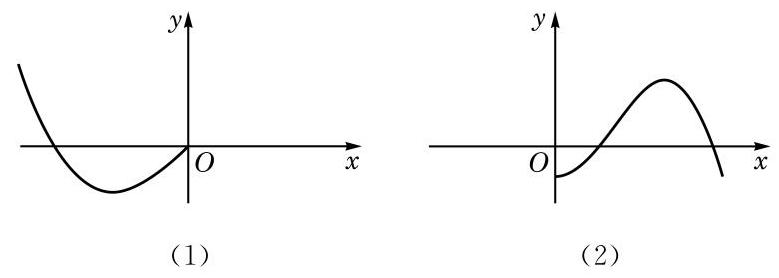
\includegraphics[max width=0.6\textwidth]{images/bo_d7fr3gc91nqc7381iccg_133_417_510_779_278_0.jpg}
\end{center}
\hspace*{3em} 

(第 2 题)

3. 证明下列函数是奇函数:

(1) \(y = {2}^{x} - {2}^{-x}\) ; (2) \(y = {\log }_{2}\left( {1 + x}\right)  - {\log }_{2}\left( {1 - x}\right)\) .

\HRule

可以从函数值的角度来猜测，也可以借助函数图像的几何直观.

\HRule

在判断一个比较复杂的函数的奇偶性的时候, 往往采取 “先猜后证”的方法.

例 4 判断下列函数的奇偶性, 并说明理由:

(1) \(y = {\left( x - 1\right) }^{2},x \in  \mathbf{R}\) ;

(2) \(y = \left\{  \begin{array}{ll} x\left( {x + 1}\right) , & x > 0, \\  x\left( {1 - x}\right) , & x < 0. \end{array}\right.\)

解 (1) 因为当 \(x = 1\) 时, \(y = 0\) ; 而当 \(x =  - 1\) 时, \(y = 4\) , 两者不相等,所以 \(y = {\left( x - 1\right) }^{2}\) 不是偶函数;

又因为 \(0 \neq   - 4\) ,所以 \(y = {\left( x - 1\right) }^{2}\) 亦不是奇函数.

综上所述，函数 \(y = {\left( x - 1\right) }^{2}\) 既不是奇函数，又不是偶函数.

(2)经试验,发现当 \(x = 1\) 时, \(y = 2\) ，而当 \(x =  - 1\) 时, \(y =  - 2\) ; 又当 \(x = {10}\) 时, \(y = {110}\) ,而当 \(x =  - {10}\) 时, \(y =  - {110}\) ; 等等. 猜测该函数可能是奇函数.

该函数的定义域为 \(\{ x \mid  x \neq  0\}\) . 记 \(g\left( x\right)  = \left\{  \begin{array}{l} x\left( {x + 1}\right) ,x > 0, \\  x\left( {1 - x}\right) ,x < 0. \end{array}\right.\)

\HRule

也可以将 \(y = g\left( x\right)\) 表示为 \(y = x\left( {1 + \left| x\right| }\right)\) , \(x \neq  0\) . 以此证明该函数是奇函数.

\HRule

对任意给定的 \(x > 0,g\left( x\right)  = x\left( {x + 1}\right)\) . 因 \(- x < 0\) ,故

\[
g\left( {-x}\right)  = \left( {-x}\right) \left\lbrack  {1 - \left( {-x}\right) }\right\rbrack   =  - x\left( {1 + x}\right)  =  - g\left( x\right) .
\]

而对任意给定的 \(x < 0,g\left( x\right)  = x\left( {1 - x}\right)\) . 因 \(- x > 0\) ,故

\section*{}

\[
g\left( {-x}\right)  = \left( {-x}\right) \left\lbrack  {1 + \left( {-x}\right) }\right\rbrack   =  - x\left( {1 - x}\right)  =  - g\left( x\right) .
\]

综上所述, \(y = g\left( x\right)\) 确实是奇函数.

例 5 是否存在正数 \(a\) ,使函数 \(y = \frac{{a}^{x} + 1}{{2}^{x}}\) 是偶函数?

解 记 \(f\left( x\right)  = \frac{{a}^{x} + 1}{{2}^{x}}\) . 由 \(f\left( 1\right)  = \frac{1 + a}{2},f\left( {-1}\right)  = \frac{2}{a} + 2\) ,若 \(y = f\left( x\right)\) 是偶函数,就应有 \(\frac{1 + a}{2} = \frac{2}{a} + 2\) . 解这个方程,得 \(a =  - 1\) (舍去) 或 \(a = 4\) . Q

\HRule

为了表明存在性, 寻找必要条件的过程不是必须表达出来的.

\HRule

因此, \(y = f\left( x\right)\) 是偶函数的一个必要条件是 \(a = 4\) .

另一方面,当 \(a = 4\) 时, \(f\left( x\right)  = \frac{{4}^{x} + 1}{{2}^{x}} = {2}^{x} + {2}^{-x}\) ,其定义域为 \(\mathbf{R}\) . 对任意给定的 \(x \in  \mathbf{R}\) ,都有 \(- x \in  \mathbf{R}\) ,并且

\[
f\left( {-x}\right)  = {2}^{-x} + {2}^{-\left( {-x}\right) } = {2}^{-x} + {2}^{x} = f\left( x\right) .
\]

因此,当 \(a = 4\) 时, \(y = f\left( x\right)\) 是偶函数.

综上所述,满足条件的正数 \(a\) 存在.

例 6 已知函数 \(y = f\left( x\right) ,x \in  \mathbf{R}\) ,且当 \(x \geq  0\) 时,

\[
f\left( x\right)  = 2{x}^{3} + {2}^{x} - 1.
\]

(1)若函数 \(y = f\left( x\right)\) 是偶函数，求 \(f\left( {-2}\right)\) ；

(2) \(y = f\left( x\right)\) 是否可能是奇函数？若可能，求 \(f\left( x\right)\) 的表达式; 若不可能, 说明理由.

解 (1) 若 \(y = f\left( x\right)\) 是偶函数,应有 \(f\left( {-2}\right)  = f\left( 2\right)\) . 而 \(f\left( 2\right)  = 2 \times  {2}^{3} + {2}^{2} - 1 = {19}\) ,因此 \(f\left( {-2}\right)  = {19}\) .

(2)若 \(y = f\left( x\right)\) 是奇函数，当 \(x < 0\) 时，应有

\[
f\left( x\right)  =  - f\left( {-x}\right)  =  - \left\lbrack  {2{\left( -x\right) }^{3} + {2}^{-x} - 1}\right\rbrack   = 2{x}^{3} - {2}^{-x} + 1.
\]

\HRule

在例 6 (2) 的解答中我们并没有验证 “当 \(x > 0\) 时, \(f\left( x\right) \; =  - f\left( {-x}\right)\) ”. 事实上，这是由“当 \(x < 0\) 时, \(f\left( {-x}\right)  =  - f\left( x\right)\) ” 所蕴涵的.

\HRule

此外,当 \(x = 0\) 时,

\[
f\left( x\right)  = 2 \times  {0}^{3} + {2}^{0} - 1 = 0 =  - f\left( {-x}\right) .
\]

因此, \(y = f\left( x\right)\) 可能是奇函数,此时

\[
f\left( x\right)  = \left\{  \begin{array}{ll} 2{x}^{3} + {2}^{x} - 1, & x \geq  0, \\  2{x}^{3} - {2}^{-x} + 1, & x < 0. \end{array}\right.
\]

\section*{练习 5.2(2)}

1. 判断下列函数的奇偶性, 并说明理由:

(1) \(y = \left| x\right|\) ；

(2) \(y = \frac{1}{1 + x} - \frac{1}{1 - x}\) ；

\section*{}

(3) \(y = {x}^{3} - x,x \in  \lbrack  - 3,3)\) ； (4) \(y = 0,x \in  \left\lbrack  {-1,1}\right\rbrack  .\)

2. 已知 \(a\) 是实数,而定义在 \(\mathbf{R}\) 上的函数 \(y = f\left( x\right)\) 的表达式为 \(f\left( x\right)  = \left| {x - a}\right|\) .

(1)是否存在实数 \(a\) ，使得 \(y = f\left( x\right)\) 是奇函数？说明理由；

(2)是否存在实数 \(a\) ,使得 \(y = f\left( x\right)\) 是偶函数? 说明理由.

\section*{2 函数的单调性}

在现实生活中, 有不少在一定范围内随着时间的增加而增加 (或减少) 的量,如自由落体运动的位移 \(s = \frac{1}{2}g{t}^{2},t \in  \left\lbrack  {0,T}\right\rbrack\) 就是如此. 作出位移 \(s\) 关于时间 \(t\) 的函数图像,如图 5-2-4 所示. 从图像上看, 随着时间的增大, 位移的确随之增大. 这就是一种单调现象. 此外, 通过一个电阻的电流随其两端电压的增大而增大；许多物质在水中的溶解度随温度的升高而增加；山区的气温随海拔高度的升高而降低等, 都是单调现象.

\begin{center}
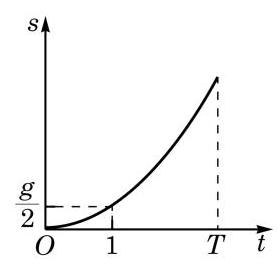
\includegraphics[max width=0.2\textwidth]{images/bo_d7fr3gc91nqc7381iccg_135_1159_693_278_264_0.jpg}
\end{center}
\hspace*{3em} 

图 5-2-4

在学习指数函数及对数函数时, 我们已经了解到如下的事实:

当 \(a > 1\) 时,函数 \(y = {a}^{x}\) 与函数 \(y = {\log }_{a}x\) 的图像都表现出 “ \(y\) 随 \(x\) 的增大而增大” 的趋势; 而当 \(0 < a < 1\) 时,函数 \(y = {a}^{x}\) 与函数 \(y = {\log }_{a}x\) 的图像却都表现出 “ \(y\) 随 \(x\) 的增大而减小” 的趋势.

图像上这样的趋势在函数性质的研究中被称为单调性, 它是函数重要的性质之一. 借助于单调性, 就能够更好地掌握函数值的变化规律.

借助指数和对数运算的性质, 必修课程第 4 章中已经证明了, 若 \({x}_{1} > {x}_{2}\) ,当 \(a > 1\) 时, \({a}^{{x}_{1}} > {a}^{{x}_{2}}\) 及 \({\log }_{a}{x}_{1} > {\log }_{a}{x}_{2}\) ; 而当 \(0 < a < 1\) 时, \({a}^{{x}_{1}} < {a}^{{x}_{2}}\) 及 \({\log }_{a}{x}_{1} < {\log }_{a}{x}_{2}\) . 这样,我们就解释了为何这些函数的图像会表现出相应的单调性趋势. 概括起来, 可对一般函数给出其单调性的定义.

定义 对于定义在 \(D\) 上的函数 \(y = f\left( x\right)\) ,设区间 \(I\) 是 \(D\) 的一个子集. 对于区间 \(I\) 上的任意给定的两个自变量的值 \({x}_{1}\text{ 、 }{x}_{2}\) , 当 \({x}_{1} < {x}_{2}\) 时,如果总有

\[
f\left( {x}_{1}\right)  \leq  f\left( {x}_{2}\right) ,
\]

就称函数 \(y = f\left( x\right)\) 在区间 \(I\) 上是增函数 (increasing function); 而

如果总有

\[
f\left( {x}_{1}\right)  \geq  f\left( {x}_{2}\right) ,
\]

就称函数 \(y = f\left( x\right)\) 在区间 \(I\) 上是减函数 (decreasing function).

Q

特别地, 如果总有

\[
f\left( {x}_{1}\right)  < f\left( {x}_{2}\right) ,
\]

就称函数 \(y = f\left( x\right)\) 在区间 \(I\) 上是严格增函数 (strictly increasing function); 而如果总有

\[
f\left( {x}_{1}\right)  > f\left( {x}_{2}\right) ,
\]

就称函数 \(y = f\left( x\right)\) 在区间 \(I\) 上是严格减函数 (strictly decreasing function).

“严格增”“严格减”“增”及“减”统称为函数的单调性.

?

例如, \(y = {2x}\) 在区间 \(\left( {-\infty , + \infty }\right)\) 上是严格增函数; \(y = {x}^{2}\) 在区间 \(( - \infty ,0\rbrack\) 上是严格减函数,在区间 \(\lbrack 0, + \infty )\) 上是严格增函数; \(y = {\log }_{2}x\) 在区间 \(\left( {0, + \infty }\right)\) 上是严格增函数; 等等.

根据已经学习过的实数幂的性质,对于幂函数 \(y = {x}^{r}\) ,当 \(r > 0\) 时,该函数在区间 \(\left( {0, + \infty }\right)\) 上是严格增函数; 而当 \(r < 0\) 时,该函数在区间 \(\left( {0, + \infty }\right)\) 上是严格减函数.

根据指数及对数的运算性质,当 \(a > 1\) 时, \(y = {a}^{x}\) 在区间 \(\left( {-\infty , + \infty }\right)\) 上是严格增函数, \(y = {\log }_{a}x\) 在区间 \(\left( {0, + \infty }\right)\) 上是严格增函数; 而当 \(0 < a < 1\) 时, \(y = {a}^{x}\) 在区间 \(\left( {-\infty , + \infty }\right)\) 上是严格减函数, \(y = {\log }_{a}x\) 在区间 \(\left( {0, + \infty }\right)\) 上是严格减函数.

例 7 证明: 函数 \(y = {x}^{2} - {2x}\) 在区间 \(( - \infty ,1\rbrack\) 上是严格减函数.

证明 记 \(f\left( x\right)  = {x}^{2} - {2x}\) . 设 \({x}_{1}\text{ 、 }{x}_{2}\) 是区间 \(( - \infty ,1\rbrack\) 上任意给定的两个实数,且 \({x}_{1} < {x}_{2}\) ,我们有

\[
f\left( {x}_{1}\right)  = {x}_{1}^{2} - 2{x}_{1},f\left( {x}_{2}\right)  = {x}_{2}^{2} - 2{x}_{2}.
\]

由于

\[
f\left( {x}_{1}\right)  - f\left( {x}_{2}\right)  = \left( {{x}_{1}^{2} - 2{x}_{1}}\right)  - \left( {{x}_{2}^{2} - 2{x}_{2}}\right)
\]

\[
= \left( {{x}_{1}^{2} - {x}_{2}^{2}}\right)  - 2\left( {{x}_{1} - {x}_{2}}\right)
\]

\[
= \left( {{x}_{1} - {x}_{2}}\right) \left( {{x}_{1} + {x}_{2} - 2}\right) \text{ , }
\]

又 \({x}_{1} - {x}_{2} < 0\) ，且 \({x}_{1} + {x}_{2} - 2 < 1 + 1 - 2 = 0\) ，故

\[
f\left( {x}_{1}\right)  - f\left( {x}_{2}\right)  > 0,
\]

即 \(f\left( {x}_{1}\right)  > f\left( {x}_{2}\right)\) .

因此,函数 \(y = {x}^{2} - {2x}\) 在区间 \(( - \infty ,1\rbrack\) 上是严格减函数.

\section*{}

\HRule

根据定义, 严格增函数是增函数, 严格减函数是减函数.

你能用定义证明初中学过的一次函数和反比例函数的单调性吗?

\HRule

对于一般的二次函数 \(y = f\left( x\right)\) ,其中 \(f\left( x\right)  = a{x}^{2} + {bx} + c \; \left( {a \neq  0}\right)\) ,通过配方法,得到

\[
f\left( x\right)  = a{\left( x + \frac{b}{2a}\right) }^{2} + \frac{{4ac} - {b}^{2}}{4a}.
\]

因此，点 \(\left( {-\frac{b}{2a},\frac{{4ac} - {b}^{2}}{4a}}\right)\) 被称为该二次函数的图像的顶点，它是相应曲线(抛物线)的最高点或最低点.

先考察 \(a > 0\) 的情形. 设 \({x}_{1}\text{ 、 }{x}_{2}\) 是任意给定的两个实数,且 \({x}_{1} < {x}_{2}\) ,我们有 \(f\left( {x}_{1}\right)  - f\left( {x}_{2}\right)  = a\left( {{x}_{1} - {x}_{2}}\right) \left\lbrack  {\left( {{x}_{1} + {x}_{2}}\right)  + \frac{b}{a}}\right\rbrack\) . 当 \({x}_{1} < {x}_{2} \leq   - \frac{b}{2a}\) 时,由 \({x}_{1} - {x}_{2} < 0\) 以及 \({x}_{1} + {x}_{2} + \frac{b}{a} < 0\) ,可得 \(f\left( {x}_{1}\right)  > f\left( {x}_{2}\right)\) ; 而当 \(- \frac{b}{2a} \leq  {x}_{1} < {x}_{2}\) 时,由 \({x}_{1} - {x}_{2} < 0\) 以及 \({x}_{1} + {x}_{2} + \frac{b}{a} > 0\) ,可得 \(f\left( {x}_{1}\right)  < f\left( {x}_{2}\right)\) .

因此,当 \(a > 0\) 时,函数 \(y = a{x}^{2} + {bx} + c\) 在区间 \(( - \infty , - \frac{b}{2a}\rbrack\) 上是严格减函数,在区间 \(\left\lbrack  {-\frac{b}{2a}, + \infty }\right)\) 上是严格增函数.

类似地,当 \(a < 0\) 时,函数 \(y = a{x}^{2} + {bx} + c\) 在区间 \(\left( {-\infty , - \frac{b}{2a}}\right\rbrack\) 上是严格增函数,在区间 \(\left\lbrack  {-\frac{b}{2a}, + \infty }\right)\) 上是严格减函数.

由上述二次函数的单调性可知, 二次函数图像的上升与下降的趋势恰好以它对应的抛物线的顶点为分界点.

例 8 判断函数 \(y = {\log }_{2}\left( {{3x} + 2}\right)\) 在其定义域上的单调性, 并说明理由.

解 设 \({x}_{1}\text{ 、 }{x}_{2}\) 是定义域 \(D = \{ x \mid  {3x} + 2 > 0\}\) 上任意给定的两个实数,且 \({x}_{1} < {x}_{2}\) ,易知 \(0 < 3{x}_{1} + 2 < 3{x}_{2} + 2\) . 因为函数 \(y = {\log }_{2}x\) 在区间 \(\left( {0, + \infty }\right)\) 上是严格增函数,所以 \({\log }_{2}\left( {3{x}_{1} + 2}\right)  < \; {\log }_{2}\left( {3{x}_{2} + 2}\right)\) .

因此, \(y = {\log }_{2}\left( {{3x} + 2}\right)\) 在其定义域上是严格增函数.

\section*{练习 5.2(3)}

1. 小明说:“如果当 \(x > 0\) 时,总有 \(f\left( x\right)  > f\left( 0\right)\) ,那么函数 \(y = f\left( x\right)\) 在区间 \(\lbrack 0, + \infty )\) 上是严格增函数. ”他的说法是否正确？说明理由.

2. 证明: 函数 \(y = \frac{2}{{x}^{3}}\) 在区间 \(\left( {-\infty ,0}\right)\) 上是严格减函数.

3. 构造一个二次函数,使得它在区间 \(\left\lbrack  {-1,1}\right\rbrack\) 上是严格减函数,并说明理由.

需要注意的是, 函数的单调性是针对包含于定义域中的某个区间而言的. 有些函数虽然在整个定义域上不是单调函数, 但是在包含于定义域中的某些区间上却可以是单调函数.

\HRule

一般来说，所讨论的单调区间总是指满足这一要求的“最大”的单调区间.

\HRule

定义 如果函数 \(y = f\left( x\right)\) 在某个区间 \(I\) 上是增 (减) 函数, 那么就称函数 \(y = f\left( x\right)\) 在区间 \(I\) 上是单调函数 (monotonic function),并称区间 \(I\) 是函数 \(y = f\left( x\right)\) 的一个单调区间.

?

例 9 判断函数 \(y = {x}^{2} - {2x},x \in  \left\lbrack  {-2,2}\right\rbrack\) 的单调性,并求出它的单调区间.

\HRule

你能用上一节课学习的一般二次函数的单调性结论来求这个函数的单调区间吗?

\HRule

解 记 \(f\left( x\right)  = {x}^{2} - {2x}.f\left( 0\right)  = f\left( 2\right)  = 0\) ,而 \(f\left( 1\right)  =  - 1\) ,因此 \(y = {x}^{2} - {2x}\) 在区间 \(\left\lbrack  {-2,2}\right\rbrack\) 上既不是增函数,也不是减函数.

对区间 \(I\) 上任意给定的两个实数 \({x}_{1}\text{ 、 }{x}_{2}\) ,总有

\[
f\left( {x}_{1}\right)  - f\left( {x}_{2}\right)  = \left( {{x}_{1} - {x}_{2}}\right) \left( {{x}_{1} + {x}_{2} - 2}\right) .
\]

当 \({x}_{1} < {x}_{2}\) ,且 \({x}_{1}\text{ 、 }{x}_{2} \in  \left\lbrack  {-2,1}\right\rbrack\) 时,总有 \({x}_{1} + {x}_{2} - 2 < 0\) 及 \({x}_{1} - {x}_{2} < 0\) ,故 \(f\left( {x}_{1}\right)  - f\left( {x}_{2}\right)  > 0\) ,从而函数 \(y = {x}^{2} - {2x}\) , \(x \in  \left\lbrack  {-2,2}\right\rbrack\) 在区间 \(\left\lbrack  {-2,1}\right\rbrack\) 上是严格减函数.

类似地,当 \({x}_{1} < {x}_{2}\) ,且 \({x}_{1}\text{ 、 }{x}_{2} \in  \left\lbrack  {1,2}\right\rbrack\) 时,总有 \({x}_{1} + {x}_{2} - \; 2 > 0\) 及 \({x}_{1} - {x}_{2} < 0\) ,故 \(f\left( {x}_{1}\right)  - f\left( {x}_{2}\right)  < 0\) ,从而函数 \(y = {x}^{2} - {2x}\) , \(x \in  \left\lbrack  {-2,2}\right\rbrack\) 在区间 \(\left\lbrack  {1,2}\right\rbrack\) 上是严格增函数.

因此，函数 \(y = {x}^{2} - {2x},x \in  \left\lbrack  {-2,2}\right\rbrack\) 的单调区间有 \(\left\lbrack  {-2,1}\right\rbrack\) 和 \(\left\lbrack  {1,2}\right\rbrack\) .

例 10 设 \(y = f\left( x\right)\) 是偶函数,且它在区间 \(\left\lbrack  {-2, - 1}\right\rbrack\) 上是严格减函数，判断它在区间 \(\left\lbrack  {1,2}\right\rbrack\) 上的单调性，并说明理由.

解 设 \({x}_{1}\text{ 、 }{x}_{2}\) 是区间 \(\left\lbrack  {1,2}\right\rbrack\) 上任意给定的两个实数,且 \({x}_{1} < {x}_{2}\) ,则 \(- {x}_{1}\text{ 、 } - {x}_{2} \in  \left\lbrack  {-2, - 1}\right\rbrack\) ,且 \(- {x}_{2} <  - {x}_{1}\) .

因为函数 \(y = f\left( x\right)\) 在区间 \(\left\lbrack  {-2, - 1}\right\rbrack\) 上是严格减函数,所以 \(f\left( {-{x}_{2}}\right)  > f\left( {-{x}_{1}}\right)\) . 又因为 \(y = f\left( x\right)\) 是偶函数,所以 \(f\left( {x}_{2}\right)  = f\left( {-{x}_{2}}\right)  > f\left( {-{x}_{1}}\right)  = f\left( {x}_{1}\right) .\)

因此, \(y = f\left( x\right)\) 在区间 \(\left\lbrack  {1,2}\right\rbrack\) 上是严格增函数.

例 10 展示了如何利用函数的奇偶性来研究函数的其他性质.

\section*{}

\section*{练习 5.2(4)}

1. 根据下列函数 \(y = f\left( x\right)\) 的图像 (包括端点),分别指出这两个函数的单调区间,以及在每一个单调区间上函数的单调性.

\begin{center}
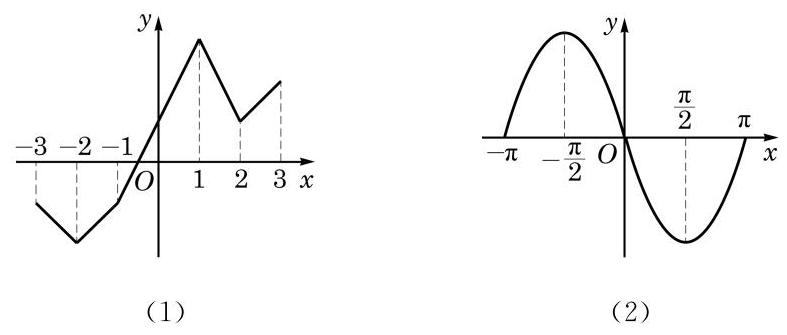
\includegraphics[max width=0.6\textwidth]{images/bo_d7fr3gc91nqc7381iccg_139_414_492_787_335_0.jpg}
\end{center}
\hspace*{3em} 

(第 1 题)

2. 判断函数 \(y = \left| {x + 1}\right| ,x \in  \left\lbrack  {-2,2}\right\rbrack\) 的单调性,并求出其单调区间.

3. 设 \(y = f\left( x\right)\) 是奇函数,且它在区间 \(( - 3,0\rbrack\) 上是严格增函数.

(1)求证:它在区间 \(\lbrack 0,3)\) 上是严格增函数；

(2) \(y = f\left( x\right)\) 是否在区间 \(\left( {-3,3}\right)\) 上是严格增函数？说明理由.

\section*{3 函数的最值}

在必修课程第 2 章中, 我们已经利用不等式的性质及基本不等式求解了一些代数式的最大值和最小值. 对于只有一个未知数的代数式,如 \(x + \frac{1}{x},{x}^{2} - {2x}\) 等,当 \(x\) 的值改变时,相应代数式的值也随之改变,从而都可以将它们看成是自变量 \(x\) 的函数. 函数值的大小变化趋势是函数的单调性研究所关心的内容. 而在生产和生活中, 除了函数值的大小变化趋势之外, 往往也关心函数何时取到最大值(最小值)，以及最大值(最小值)为多少等问题.

\HRule

最大值与最小值统称为最值.

\HRule

定义 函数 \(y = f\left( x\right)\) 在定义域内的 \({x}_{0}\) 处的函数值是 \(f\left( {x}_{0}\right)\) ,对于定义域内任意给定的 \(x\) ,如果

\[
f\left( x\right)  \geq  f\left( {x}_{0}\right)
\]

都成立,那么 \(f\left( {x}_{0}\right)\) 就叫做函数 \(y = f\left( x\right)\) 的最小值 (minimum);

相反, 如果

\[
f\left( x\right)  \leq  f\left( {x}_{0}\right)
\]

都成立,那么 \(f\left( {x}_{0}\right)\) 就叫做函数 \(y = f\left( x\right)\) 的最大值 (maximum).

例 11 求函数 \(y = 2{x}^{2} - {3x} + 1,x \in  \mathbf{R}\) 的最大值与最小值.

解 由于 \(y = 2{x}^{2} - {3x} + 1 = 2{\left( x - \frac{3}{4}\right) }^{2} - \frac{1}{8} \geq   - \frac{1}{8}\) ,且当 \(x = \frac{3}{4}\) 时上述不等式中的等号可以取到,因此该函数的最小值为 \(- \frac{1}{8}\) .

由二次函数的单调性可知, 该函数无最大值.

对于定义在闭区间 \(\left\lbrack  {a,b}\right\rbrack\) 上的单调函数 \(y = f\left( x\right)\) ,它的最大值和最小值一定能在区间的端点 \(a\) 和 \(b\) 处取到. 因此,对于具有单调性的函数, 可以借助其单调性来求得其最值.

例 12 求函数 \(y = \frac{2}{x},x \in  \left\lbrack  {1,2}\right\rbrack\) 的最大值与最小值.

解 由于函数 \(y = \frac{2}{x}\) 在区间 \(\left\lbrack  {1,2}\right\rbrack\) 上是严格减函数,因此, 其最大值在左端点 \(x = 1\) 处取到,其值为 2 ; 而最小值在右端点 \(x = 2\) 处取到，其值为 1 .

例 13 已知 \(a < 2\) ,求函数 \(y = \left| {x - 1}\right| ,x \in  \left\lbrack  {a,2}\right\rbrack\) 的最大值.

解 对于函数 \(y = \left| {x - 1}\right|\) ,当 \(x \geq  1\) 时, \(y = x - 1\) ; 而当 \(x \leq  1\) 时, \(y =  - x + 1\) . 因此, \(y = \left| {x - 1}\right|\) 在区间 \(\lbrack 1, + \infty )\) 上是严格增函数,在区间 \(( - \infty ,1\rbrack\) 上是严格减函数.

情形一: 当 \(1 \leq  a < 2\) 时, \(y = \left| {x - 1}\right|\) 在区间 \(\left\lbrack  {a,2}\right\rbrack\) 上是严格增函数,如图 5-2-5(1)所示. 此时函数的最大值为 1 .

情形二: 当 \(a < 1\) 时, \(y = \left| {x - 1}\right|\) 在区间 \(\left\lbrack  {a,1}\right\rbrack\) 上是严格减函数,而在区间 \(\left\lbrack  {1,2}\right\rbrack\) 上是严格增函数,如图 5-2-5(2)所示. 从而此时函数的最大值为 \(\left| {2 - 1}\right|\) 与 \(\left| {a - 1}\right|\) 中的较大者. 因此,当 \(a < 0\) 时,该函数的最大值为 \(\left| {a - 1}\right|  = 1 - a\) ; 而当 \(0 \leq  a < 1\) 时,该函数的最大值为 1 .

\section*{}

\begin{center}
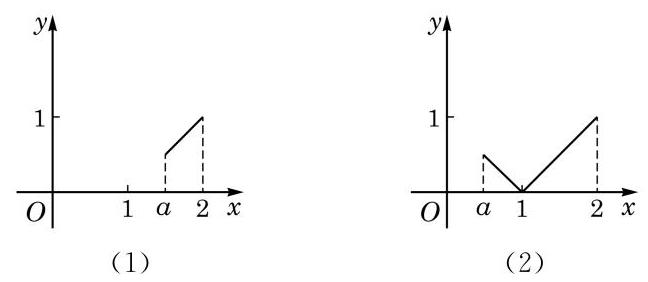
\includegraphics[max width=0.5\textwidth]{images/bo_d7fr3gc91nqc7381iccg_141_300_230_648_282_0.jpg}
\end{center}
\hspace*{3em} 

图 5-2-5

综上所述,当 \(a < 0\) 时,该函数的最大值为 \(1 - a\) ; 当 \(0 \leq  a < 2\) 时,该函数的最大值为 1 .

\section*{练习 5.2(5)}

1. 求函数 \(y = {\left( \frac{1}{2}\right) }^{x},x \in  \left\lbrack  {1,3}\right\rbrack\) 的最大值与最小值.

2. 求下列函数的最大值与最小值:

(1) \(y = 1 - {x}^{2}\) ； (2) \(y = 1 - {x}^{2},x \in  \left\lbrack  {-1,2}\right\rbrack\) ；

(3) \(y = {2{x}^{2}} - {8x}\) ； (4) \(y = 2{x}^{2} - {8x},x \in  \left\lbrack  {0,1}\right\rbrack  .\)

3. 已知 \(a >  - 2\) ,求函数 \(y = {x}^{2} + 1,x \in  \left\lbrack  {-2,a}\right\rbrack\) 的最大值.

\section*{习题 5.2}

\section*{A 组}

1. 若函数 \(y = f\left( x\right)\) 的定义域为 \(\mathbf{R}\) ,则 \(y = f\left( x\right)\) 为奇函数的充要条件为 ( )

A. \(f\left( 0\right)  = 0\) ;

B. 对任意 \(x \in  \mathbf{R},f\left( x\right)  = 0\) 都成立;

C. 存在某个 \({x}_{0} \in  \mathbf{R}\) ,使得 \(f\left( {x}_{0}\right)  + f\left( {-{x}_{0}}\right)  = 0\) ;

D. 对任意给定的 \(x \in  \mathbf{R},f\left( x\right)  + f\left( {-x}\right)  = 0\) 都成立.

2. 证明下列函数 \(y = f\left( x\right)\) 为偶函数:

(1) \(f\left( x\right)  = {x}^{2} + {x}^{-2}\) ；

(2) \(f\left( x\right)  = \frac{x\left( {{2}^{x} - 1}\right) }{{2}^{x} + 1}\) .

3. 证明下列函数 \(y = f\left( x\right)\) 为奇函数:

(1) \(f\left( x\right)  = {x}^{-3}\) ； (2) \(f\left( x\right)  = \frac{{\mathrm{e}}^{x} - {\mathrm{e}}^{-x}}{2}\) .

4. 判断下列函数 \(y = f\left( x\right)\) 的奇偶性,并说明理由:

\section*{}



(1) \(f\left( x\right)  = {2x} + \sqrt[3]{x}\) ； (2) \(f\left( x\right)  = 2{x}^{4} - {x}^{2}\) ；

(3) \(f\left( x\right)  = {x}^{2} - x\) ;

(4) \(f\left( x\right)  = \frac{1 - x}{1 + x}\) ；

(5) \(f\left( x\right)  = \lg \frac{1 - x}{1 + x}\) .

5. 证明: 函数 \(y = x - \frac{1}{x},x \in  \left( {-\infty ,0}\right)\) 是严格增函数.

6. 证明: 函数 \(y = \lg \left( {1 - x}\right)\) 在其定义域上是严格减函数.

7. 求下列函数的最大值与最小值, 并写出取最值时相应自变量的值:

(1) \(y = {x}^{2} - {4x} - 2\) ;

(2) \(y = {6x} - 3{x}^{2}\) ；

(3) \(y =  - {x}^{2} - {4x} - 3,x \in  \left\lbrack  {-3,1}\right\rbrack\) ；

(4) \(y = {x}^{2} - {2x} - 3,x \in  \left\lbrack  {-2,0}\right\rbrack\) .

8. 求函数 \(y = {\log }_{\frac{1}{2}}\left( {x + 2}\right) ,x \in  \left\lbrack  {2,6}\right\rbrack\) 的最大值与最小值.

9. 已知 \(y = {x}^{2} + {px} + q\) 和 \(y = x + \frac{4}{x}\) 都是定义在 \(\left\lbrack  {1,4}\right\rbrack\) 上的函数,且在 \({x}_{0}\) 处同时取到相同的最小值. 求 \(y = {x}^{2} + {px} + q\) 的最大值.

\section*{B 组}

1. 已知实数 \(b < 2\) ,而函数 \(y = {x}^{2} + {ax} + 1,x \in  \left\lbrack  {b,2}\right\rbrack\) 是偶函数. 求实数 \(a\text{ 、 }b\) 的值.

2. 判断下列函数 \(y = f\left( x\right)\) 的奇偶性,并说明理由:

(1) \(f\left( x\right)  = \frac{{10}^{x} - {10}^{-x}}{{10}^{x} + {10}^{-x}}\) ; (2) \(f\left( x\right)  = x\left( {\frac{1}{{2}^{x} - 1} + \frac{1}{2}}\right)\) .

3. 当表达式 \(f\left( x\right)  =\) \_\_\_\_\_时，函数 \(y = f\left( x\right)\) 同时满足以下条件:

 \circled{1}  不是偶函数；

 \circled{2}  在区间 \(\left( {-\infty , - 1}\right)\) 上是严格减函数；

 \circled{3}  在区间 \(\left( {0,1}\right)\) 上是严格增函数.

4. 作出函数 \(y = {x}^{2} - 2\left| x\right|\) 的大致图像,并分别写出它的定义域、奇偶性、单调区间及最小值.

5. 研究函数 \(y = \frac{1}{1 + {x}^{2}}\) 的定义域、奇偶性、单调性及最大值.

6. 如果函数 \(y = {x}^{2} - {2m}x + 1\) 在区间 \(( - \infty ,2\rbrack\) 上是严格减函数，那么实数 \(m\) 的取值范围为\_\_\_\_\_.

7. 设 \(t\) 是实数,且 \(t < 4\) . 求函数 \(y = \left| {{2}^{x + 1} - 8}\right| ,x \in  \left\lbrack  {t,4}\right\rbrack\) 的最小值.

\section*{5.3 函数的应用}

\section*{1 函数关系的建立}

\begin{center}
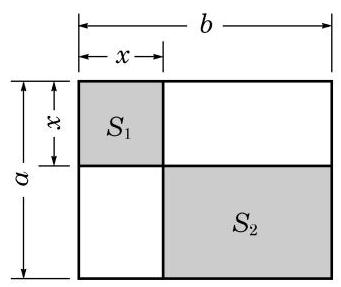
\includegraphics[max width=0.2\textwidth]{images/bo_d7fr3gc91nqc7381iccg_143_1134_732_341_287_0.jpg}
\end{center}
\hspace*{3em} 

图 5-3-1

在研究某些数学问题时, 所研究的变量往往依赖于另一个变量, 此时就需要建立这两个变量之间的函数关系.

例 1 如图 5-3-1,一个边长为 \(a\text{ 、 }b\left( {a < b}\right)\) 的长方形被分别平行于长与宽的两条直线所分割, 试用解析法将图中阴影部分的总面积 \(S\) 表示为 \(x\) 的函数.

解 因为左上角阴影部分的面积 \({S}_{1} = {x}^{2}\) ,而右下角阴影部分的面积 \({S}_{2} = \left( {a - x}\right) \left( {b - x}\right)\) ,所以阴影部分的总面积

\[
S = {S}_{1} + {S}_{2} = {x}^{2} + \left( {a - x}\right) \left( {b - x}\right) .
\]

\begin{center}
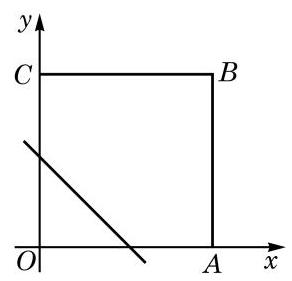
\includegraphics[max width=0.2\textwidth]{images/bo_d7fr3gc91nqc7381iccg_143_1154_1142_292_281_0.jpg}
\end{center}
\hspace*{3em} 

图 5-3-2

因此,所求函数为 \(S = 2{x}^{2} - \left( {a + b}\right) x + {ab},x \in  \left( {0,a}\right)\) .

例 2 如图 5-3-2,四边形 \({OABC}\) 是平面直角坐标系中边长为 1 的正方形. 一直线 \(y =  - x + t\left( {t \in  \left( {0,2}\right) }\right)\) 与正方形 \({OABC}\) 相交,将正方形分为两个部分,其中包含原点 \(O\) 的部分的面积记为 \(S\) . 试将 \(S\) 表示为 \(t\) 的函数.

\begin{center}
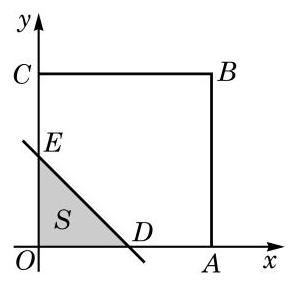
\includegraphics[max width=0.2\textwidth]{images/bo_d7fr3gc91nqc7381iccg_143_1155_1478_291_281_0.jpg}
\end{center}
\hspace*{3em} 

图 5-3-3

解 \(t\) 是直线 \(y =  - x + t\) 在 \(y\) 轴上的截距.

情形一:当 \(0 < t \leq  1\) 时，设该直线与线段 \({OC}\) 交于点 \(E\) ，并与线段 \({OA}\) 交于点 \(D\) ,如图 5-3-3 所示.

此时,包含点 \(O\) 的部分是直角三角形 \({ODE}\) . 由于 \({OD} = {OE} \; = t\) ,因此

\[
S = \frac{1}{2}{OD} \cdot  {OE} = \frac{1}{2}{t}^{2}.
\]

\begin{center}
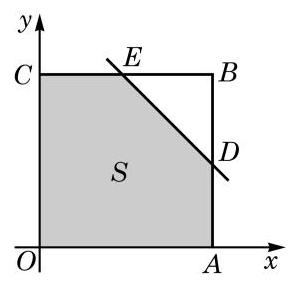
\includegraphics[max width=0.2\textwidth]{images/bo_d7fr3gc91nqc7381iccg_143_1154_1813_292_281_0.jpg}
\end{center}
\hspace*{3em} 

图 5-3-4

情形二: 当 \(1 < t < 2\) 时,设该直线与线段 \({BC}\) 交于点 \(E\) ,并与线段 \({AB}\) 交于点 \(D\) ,如图 5-3-4 所示.

此时,包含点 \(O\) 的部分是五边形 \({OADEC}\) ,它可以看成是正方形 \({OABC}\) 除去直角三角形 \({BDE}\) 所得的部分,由于 \({BD} = {BE} = \; 2 - t\) ,因此

\[
S = {OA} \cdot  {OC} - \frac{1}{2}{BD} \cdot  {BE} = 1 - \frac{1}{2}{\left( 2 - t\right) }^{2} =  - \frac{1}{2}{t}^{2} + {2t} - 1.
\]



综上所述,可以分段表示 \(S\) 关于 \(t\) 的函数如下:

\[
S = \left\{  \begin{array}{ll} \frac{1}{2}{t}^{2}, & 0 < t \leq  1, \\   - \frac{1}{2}{t}^{2} + {2t} - 1, & 1 < t < 2. \end{array}\right.
\]

当我们用数学方法解决实际问题时, 首先要把问题中的有关变量及其关系表示出来, 这显示了建立变量之间的函数关系的重要性.

例 3 要建造一面靠墙、且面积相同的两间相邻的长方形居室，如图 5-3-5 所示. 如果已有材料可建成的围墙总长度为 \({30}\mathrm{\;m}\) ,那么当宽 \(x\) (单位: \(\mathrm{m}\) ) 为多少时,才能使所建造的居室总面积最大？居室的最大总面积是多少？

\begin{center}
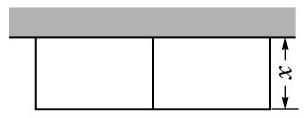
\includegraphics[max width=0.2\textwidth]{images/bo_d7fr3gc91nqc7381iccg_144_195_652_305_118_0.jpg}
\end{center}
\hspace*{3em} 

图 5-3-5

解 由题意,应有 \(0 < x < {10}\) .

如果把建筑材料全部用完, 那么此两间居室的总长应为 \(\left( {{30} - {3x}}\right) \mathrm{m}\) .

设居室的总面积为 \(y{\mathrm{\;m}}^{2}\) ,则

\[
y = x\left( {{30} - {3x}}\right)  =  - 3{\left( x - 5\right) }^{2} + {75},0 < x < {10}.
\]

所以,当居室的宽为 \(5\mathrm{\;m}\) 时,其总面积最大,且最大总面积为 \({75}{\mathrm{\;m}}^{2}\) .

\begin{center}
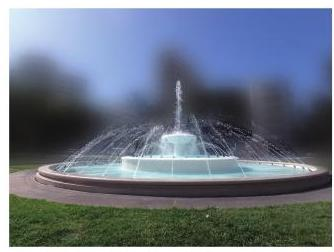
\includegraphics[max width=0.2\textwidth]{images/bo_d7fr3gc91nqc7381iccg_144_179_1259_334_252_0.jpg}
\end{center}
\hspace*{3em} 

例 4 某小区要建造一个直径为 \({16}\mathrm{\;m}\) 的圆形喷水池,并在池的周边靠近水面的位置安装一圈喷水头，使喷出的水柱在离池中心 \(3\mathrm{\;m}\) 的地方达到最高高度 \(4\mathrm{\;m}\) . 各方向喷来的水柱在池中心上方某一点汇合, 求该点离水面的高度.

解 过水池的中心任取一个竖直截面，如图 5-3-6 所示. 根据力学的原理, 喷出的水珠轨迹应为一条抛物线, 此抛物线上任何一个点距池中心的水平距离与其所处的高度之间是对应的. 为了建立水平距离 \(x\) (单位: \(\mathrm{m}\) ) 与离水面的高度 \(y\) (单位: \(\mathrm{m}\) ) 之间的函数关系 \(y = f\left( x\right)\) ,建立如图 5-3-6 所示的直角坐标系.

\begin{center}
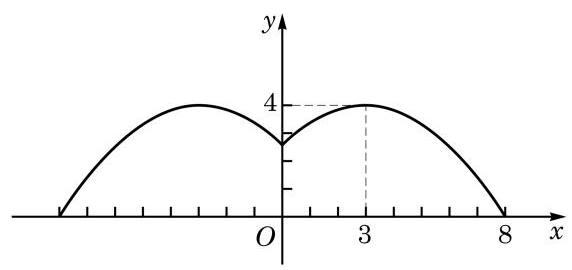
\includegraphics[max width=0.4\textwidth]{images/bo_d7fr3gc91nqc7381iccg_144_736_1779_572_270_0.jpg}
\end{center}
\hspace*{3em} 

图 5-3-6

\section*{}

设图中右半部分的曲线所对应的函数表达式为

\[
y =  - a{\left( x - b\right) }^{2} + c,0 \leq  x \leq  8,
\]

其中点 \(\left( {b,c}\right)\) 是此抛物线的顶点. 由题意,可得 \(b = 3,c = 4\) .

又由 \(f\left( 8\right)  = 0\) ,解得 \(a = {0.16}\) .

这样，该汇合点离水面的高度应为

\[
h = f\left( 0\right)  =  - {0.16} \times  {\left( 0 - 3\right) }^{2} + 4 = {2.56}\left( \mathrm{\;m}\right) .
\]

\section*{练习 5.3(1)}

1. 已知一等腰三角形的周长为 \({12}\mathrm{\;{cm}}\) ，试将该三角形的腰长 \(y\) (单位: \(\mathrm{{cm}}\) )表示为底边长 \(x\) (单位: \(\mathrm{{cm}}\) ) 的函数.

2. 如图，在平面直角坐标系的第一象限内， \(\bigtriangleup  {OAB}\) 是边长为 2 的等边三角形. 用直线 \(l : x = t\left( {0 < t < 2}\right)\) 截这个三角形,记截得的靠近 \(y\) 轴的部分的面积为 \(S\) . 试将 \(S\) 表示为 \(t\) 的函数.

\begin{center}
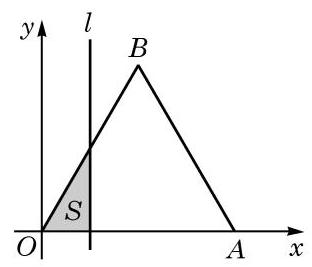
\includegraphics[max width=0.2\textwidth]{images/bo_d7fr3gc91nqc7381iccg_145_652_934_312_267_0.jpg}
\end{center}
\hspace*{3em} 

(第 2 题)

3. 某商场购物优惠活动如下:一次购物总额不超过 500 元的不予优惠；一次购物总额超过 500 元但不超过 1000 元的, 按标价给予 9 折优惠; 一次购物总额超过 1000 元的, 其中的 1000 元按上述标准给予优惠, 而超过 1000 元的部分给予 7 折优惠. 设某位顾客一次购物总额为 \(x\) 元,而优惠后实际付款额为 \(y\) 元. 试写出 \(y\) 关于 \(x\) 的函数关系.

\section*{2 用函数观点求解方程与不等式}

我们知道: 一元一次方程总可以化简为 \({ax} + b = 0\) 的形式, 而一元二次方程总可以化简为 \(a{x}^{2} + {bx} + c = 0\) 的形式. 一般地, 在求解含有一个未知数的方程时, 经过适当地化简, 总可以化为在一定的范围 \(D\) 内求解形如 \(f\left( x\right)  = 0\) 的方程,这里 \(y = f\left( x\right)\) , \(x \in  D\) 是一个函数.

在学习了函数及其性质之后, 我们可用函数的观点来考察方程 \(f\left( x\right)  = 0\) 的求解.

定义 对于函数 \(y = f\left( x\right) ,x \in  D\) ,如果存在实数 \(c \in  D\) ,使得

\[
f\left( c\right)  = 0,
\]

就把 \(c\) 叫做该函数的零点 (zero).

函数 \(y = f\left( x\right) ,x \in  D\) 的零点,就是方程 \(f\left( x\right)  = 0\) 在集合 \(D\) 中的解,也是该函数 \(y = f\left( x\right)\) 的图像与 \(x\) 轴的交点的横坐标. 这就将方程 \(f\left( x\right)  = 0\) 的求解与求函数 \(y = f\left( x\right)\) 的零点联系起来.

例 5 方程 \({x}^{3} + {2x} = {99}\) 是否有整数解? 说明理由.

解 记 \(f\left( x\right)  = {x}^{3} + {2x} - {99}\) .

对任意给定的 \({x}_{1}\text{ 、 }{x}_{2} \in  \mathbf{R}\) ,当 \({x}_{1} < {x}_{2}\) 时,根据不等式的性质,可得 \({x}_{1}^{3} < {x}_{2}^{3}\) ,并且 \(2{x}_{1} < 2{x}_{2}\) ,因此 \(f\left( {x}_{1}\right)  < f\left( {x}_{2}\right)\) ,故函数 \(y = f\left( x\right)\) 在其定义域上是一个严格增函数.

经计算, 得

\[
f\left( 4\right)  =  - {27} < 0,f\left( 5\right)  = {36} > 0.
\]

由单调性可知,当 \(n \in  \mathbf{Z}\) ,且 \(n < 4\) 时, \(f\left( n\right)  < f\left( 4\right)  < 0\) ; 而当 \(n \in  \mathbf{Z}\) ,且 \(n > 5\) 时, \(f\left( n\right)  > f\left( 5\right)  > 0\) .

因此,任一整数一定不是函数 \(y = {x}^{3} + {2x} - {99}\) 的零点,从而方程 \({x}^{3} + {2x} = {99}\) 没有整数解.

从上述解答的过程中可以看到, 原先在解方程时, 我们的观点是静态的, 而一旦引入函数的观点, 就可以利用函数的性质尝试用动态的观点审视方程的求解了.

在必修课程第 2 章中, 我们已经学过解一元二次不等式. 现在我们同样可以用函数的观点来审视一元二次不等式的求解.

我们在必修课程第 2 章中已经知道, 对于一元二次不等式

\[
a{x}^{2} + {bx} + c > 0\left( {a > 0}\right) ,
\]

可先考察它对应的方程 \(a{x}^{2} + {bx} + c = 0\) ,而该方程的解集可能有两个元素, 可能只有一个元素, 也可能为空集.

这个图像可以帮助我们回忆二次函数的单调性. 根据本章 5.2 节中关于二次函数单调性的结论,函数 \(y = a{x}^{2} + {bx} + c\) 在区间 \(( - \infty , - \frac{b}{2a}\rbrack\) 上是严格减函数,而在区间 \(\left\lbrack  {-\frac{b}{2a}, + \infty }\right)\) 上

\begin{center}
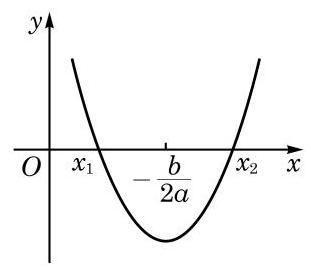
\includegraphics[max width=0.2\textwidth]{images/bo_d7fr3gc91nqc7381iccg_146_191_1790_311_270_0.jpg}
\end{center}
\hspace*{3em} 

图 5-3-7

记 \(\Delta  = {b}^{2} - {4ac}\) . 当 \(\Delta  > 0\) 时,该方程的解集可记为 \(\left\{  {{x}_{1},{x}_{2}}\right\}\) , 其中 \({x}_{1} < {x}_{2}\) . 此时函数 \(y = a{x}^{2} + {bx} + c\) 的大致图像如图 5-3-7 所示.

是严格增函数.

此外, \({x}_{1}\) 及 \({x}_{2}\) 是该函数的两个零点; 在图像上, \({x}_{1}\) 及 \({x}_{2}\) 是相应抛物线与 \(x\) 轴的交点的横坐标,且 \(\frac{{x}_{1} + {x}_{2}}{2} =  - \frac{b}{2a}\) .

这样,求解不等式 \(a{x}^{2} + {bx} + c > 0\left( {a > 0}\right)\) ,就是要求函数 \(y = a{x}^{2} + {bx} + c\left( {a > 0}\right)\) 的图像上位于 \(y > 0\) 部分的所有点的横坐标. 因此, 根据单调性及零点的位置, 参照函数的图像, 可以很容易地得到不等式 \(a{x}^{2} + {bx} + c > 0\left( {a > 0}\right)\) 的解集为 \(\left( {-\infty ,{x}_{1}}\right)  \cup \; \left( {{x}_{2}, + \infty }\right)\) . 由此可见,借助于构造一个与不等式有关的函数, 如果这个函数的单调性与零点比较容易确定, 就可以较便捷地求解相应的不等式.

这样, 可将二次项系数为正的一元二次不等式的解集总结如下.

表 5-2 二次项系数 \(a > 0\) 时,二次不等式与相应二次函数的联系

\begin{center}
\adjustbox{max width=\textwidth}{
\begin{tabular}{|c|c|c|c|}
\hline
\(f\left( x\right)  = a{x}^{2} + {bx} + c\) & \({b}^{2} - {4ac} > 0\) & \({b}^{2} - {4ac} = 0\) & \({b}^{2} - {4ac} < 0\) \\
\cline{1-4}
零点 & \({x}_{1}\text{ 、 }{x}_{2}\left( {{x}_{1} < {x}_{2}}\right)\) & \({x}_{0}\) & 不存在 \\
\cline{1-4}
大致图像 & 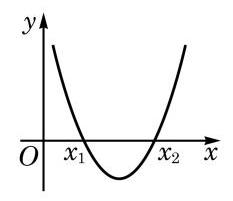
\includegraphics[max width=0.2\textwidth]{images/bo_d7fr3gc91nqc7381iccg_147_424_1210_233_201_0.jpg} & 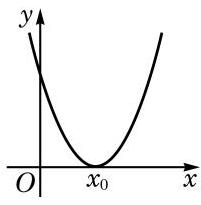
\includegraphics[max width=0.2\textwidth]{images/bo_d7fr3gc91nqc7381iccg_147_678_1209_201_205_0.jpg} & 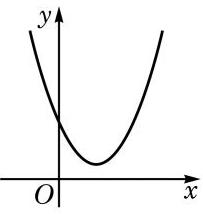
\includegraphics[max width=0.2\textwidth]{images/bo_d7fr3gc91nqc7381iccg_147_891_1203_203_214_0.jpg} \\
\cline{1-4}
\(f\left( x\right)  > 0\) 的解集 & \(\left( {-\infty ,{x}_{1}}\right)  \cup  \left( {{x}_{2}, + \infty }\right)\) & \(\left\{  {x \mid  x \neq  {x}_{0}}\right\}\) & \(\mathbf{R}\) \\
\cline{1-4}
\(f\left( x\right)  < 0\) 的解集 & \(\left( {{x}_{1},{x}_{2}}\right)\) & \(\varnothing\) & \(\varnothing\) \\
\cline{1-4}
\hline
\end{tabular}
}
\end{center}

例 6 用函数的观点在区间 \(\left( {0, + \infty }\right)\) 上解不等式 \({x}^{4} + x > 2\) .

解 记 \(f\left( x\right)  = {x}^{4} + x\) .

对任意给定的 \({x}_{1}\text{ 、 }{x}_{2} \in  \left( {0, + \infty }\right)\) ,当 \(0 < {x}_{1} < {x}_{2}\) 时,有 \({x}_{1}^{4} < {x}_{2}^{4}\) ,故

\[
{x}_{1}^{4} + {x}_{1} < {x}_{2}^{4} + {x}_{2}.
\]

因此, \(y = f\left( x\right)\) 在区间 \(\left( {0, + \infty }\right)\) 上是严格增函数.

由函数 \(y = f\left( x\right)\) 的单调性,并注意到 \(f\left( 1\right)  = {1}^{4} + 1 = 2\) ,可知在区间 \(\left( {0, + \infty }\right)\) 上, \(f\left( x\right)  > 2\) 当且仅当 \(x > 1\) .

因此,在区间 \(\left( {0, + \infty }\right)\) 上不等式 \({x}^{4} + x > 2\) 的解集为 \(\left( {1, + \infty }\right)\) .



\section*{练习 5.3(2)}

1. 利用函数与不等式的关系,在 \(a < 0\) 时,求解实系数一元二次不等式 \(a{x}^{2} + {bx} + \; c \leq  0\) .

2. 用函数的观点解不等式: \({2}^{x} + {\log }_{2}x > 2\) .

\section*{3 用二分法求函数的零点}

在建立了函数关系后, 常常会遇到一些解方程的问题. 如果相应的函数是一次函数或者二次函数，就可以用已经学习过的求根公式来求解. 但是遇到一些更复杂的函数, 相应的方程如何求解呢? 此时, 要求得问题的精确解答, 通常是做不到的, 而基于实际问题的需要, 往往只要求得具有足够精度的近似解就可以了. 本课我们将利用上一节课的思想，将求方程的近似解的问题转化为求函数的近似零点的问题, 再利用函数的性质来求得方程的近似解.

我们来看一个例子:在一块边长为 \({13}\mathrm{\;{cm}}\) 的正方形金属薄片的四个角上都剪去一个边长为 \(x\mathrm{\;{cm}}\) 的小正方形,做成一个容积是 \({140}{\mathrm{\;{cm}}}^{3}\) 的无盖长方体盒子,如图 5-3-8 所示 (图中单位: \(\mathrm{{cm}})\) . 问: \(x\) 是多少? (结果精确到 \({0.1}\mathrm{\;{cm}}\) )

\begin{center}
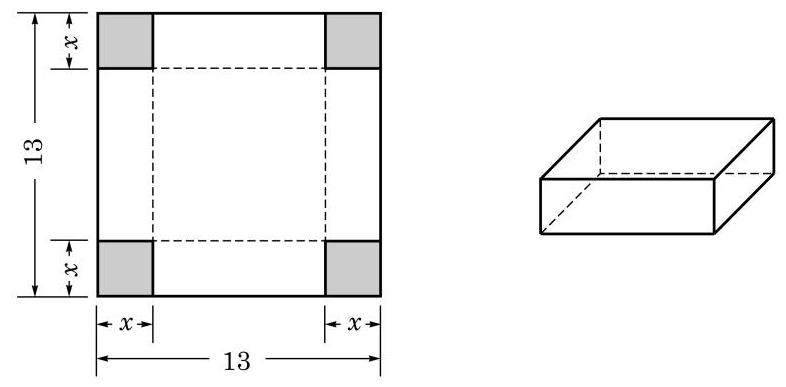
\includegraphics[max width=0.6\textwidth]{images/bo_d7fr3gc91nqc7381iccg_148_629_1437_786_387_0.jpg}
\end{center}
\hspace*{3em} 

图 5-3-8

根据要求,得 \(x{\left( {13} - 2x\right) }^{2} = {140}\) ,我们的目标就是求该方程在区间 \(\left( {0,\frac{13}{2}}\right)\) 上的实根.

令 \(f\left( x\right)  = x{\left( {13} - 2x\right) }^{2} - {140},0 < x < \frac{13}{2}\) . 上述方程的实根就



\section*{}

是函数 \(y = f\left( x\right)\) 的零点,先用描点法作出该函数的大致图像如下:

\begin{center}
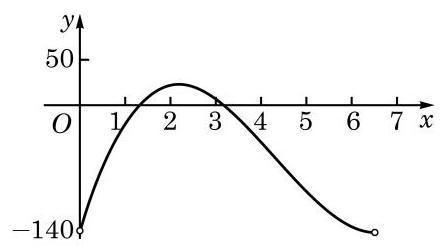
\includegraphics[max width=0.3\textwidth]{images/bo_d7fr3gc91nqc7381iccg_149_404_306_441_248_0.jpg}
\end{center}
\hspace*{3em} 

图 5-3-9

从图像上可以看出,函数 \(y = f\left( x\right)\) 在区间 \(\left( {1,2}\right)\) 和区间 (3,4)上各有一个零点.

定理 如果在区间 \(\left\lbrack  {a,b}\right\rbrack\) 上,函数 \(y = f\left( x\right)\) 的图像是一段连续曲线,并且 \(f\left( a\right)  \cdot  f\left( b\right)  < 0\) ,那么 \(y = f\left( x\right)\) 在区间 \(\left( {a,b}\right)\) 上一定有零点.

下面用二分法寻求该函数在区间 \(\left( {3,4}\right)\) 上的零点的近似值.

二分法的思想非常直接和简单: 在确定了区间 \(\left( {a,b}\right)\) 上一定有零点的前提下, 将区间一分为二, 这两部分中总有一个含有零点, 而含有零点的区间的长度变为原先的一半. 反复执行这种 “一分为二”的操作，就能将零点限制在一个足够小的区间中，从而容易求得其近似值了.

因为 \(f\left( 3\right)  = 7 > 0,f\left( 4\right)  =  - {40} < 0\) ,所以此函数 \(y = f\left( x\right)\) 在区间 \(\left( {3,4}\right)\) 上至少有一个有零点.

取 \(\left( {3,4}\right)\) 的中点 \({x}_{1} = \frac{3 + 4}{2} = {3.5}\) ,计算可得 \(f\left( {3.5}\right)  =  - {14} < 0\) . 因为 \(f\left( 3\right)  \cdot  f\left( {3.5}\right)  < 0\) ,所以 \(y = f\left( x\right)\) 在区间 \(\left( {3,{3.5}}\right)\) 上一定有零点.

将这一步骤重复若干次, 见表 5-3:

表 5-3 用二分法求函数零点的一个例子

\begin{center}
\adjustbox{max width=\textwidth}{
\begin{tabular}{|c|c|c|c|c|c|c|}
\hline
步骤 & L(左端点) & \(M\) (中点) & \(R\) (右端点) & \(f\left( L\right)\) & \(f\left( M\right)\) & \(f\left( R\right)\) \\
\cline{1-7}
1 & 3 & 3.5 & 4 & + & - & - \\
\cline{1-7}
2 & 3 & 3.25 & 3.5 & + & - & - \\
\cline{1-7}
3 & 3 & 3.125 & 3.25 & + & + & - \\
\cline{1-7}
4 & 3.125 & 3.1875 & 3.25 & + & - & - \\
\cline{1-7}
5 & 3.125 & 3.15625 & 3.1875 & + & + & - \\
\cline{1-7}
\hline
\end{tabular}
}
\end{center}

\HRule

我们学过的一次函数、二次函数、反比例函数、幂函数、 指数函数、对数函数以及必修课程第 7 章将要学习的三角函数等，在包含于定义域的任一区间上，图像都是连续的曲线.

\HRule



注意到区间 \(\left( {{3.15625},{3.1875}}\right)\) 中的所有数精确到 0.1 时的近似值都是 3.2,所以 \(y = f\left( x\right)\) 在区间 \(\left( {3,4}\right)\) 上零点的近似值是 3.2 .

按同样的操作方法,可以求得 \(y = f\left( x\right)\) 在区间 \(\left( {1,2}\right)\) 上的零点近似值是 1.3 .

综上所述,上述问题中所剪去的小正方形的边长约是 \({1.3}\mathrm{\;{cm}}\) 或 \({3.2}\mathrm{\;{cm}}\) .

可以看到, 在二分法的实际操作中, 从第二步起, 每一步只需要计算一个函数值, 并判断它的符号, 同时, 所考虑的区间长度减半.

二分法的这些步骤中, 每一步都是明确的. 尽管每一步的计算可能不一定简单, 而且可能需要重复较多的步骤才能得到具有足够精度的零点近似值, 但根据这一算法不断重复同一类计算的特点, 可利用计算机强大的计算功能, 通过编制计算机程序, 很高效地求出零点的近似值. ?

\HRule

有兴趣的同学可以设计一个二分法求函数零点的程序.

\HRule

\section*{练习 5.3(3)}

1. 对于在区间 \(\left\lbrack  {a,b}\right\rbrack\) 上的图像是一段连续曲线的函数 \(y = f\left( x\right)\) ,如果 \(f\left( a\right)  \cdot  f\left( b\right)  > 0\) , 那么是否该函数在区间 \(\left( {a,b}\right)\) 上一定无零点? 说明理由.

2. 已知函数 \(y = 2{x}^{3} - 3{x}^{2} - {18x} + {28}\) 在区间 \(\left( {1,2}\right)\) 上有且仅有一个零点. 试用二分法求出该零点的近似值. (结果精确到 0.1)

\section*{习题 5.3}

\section*{A 组}

1. 某企业去年四个季度生产某种型号机器的数量 \(y\) (单位:万台) 与季度 \(x\) 的函数关系如下表所示:

\begin{center}
\adjustbox{max width=\textwidth}{
\begin{tabular}{|c|c|c|c|c|}
\hline
\(x/\) 季度 & 1 & 2 & 3 & 4 \\
\cline{1-5}
\(y\) /万台 & 10 & 12 & 14 & 16 \\
\cline{1-5}
\hline
\end{tabular}
}
\end{center}

试写出该函数的定义域, 并作出其大致图像.

2. 某地区住宅电话费收取标准为:接通后 3 分钟内(含 3 分钟)收费 0.20 元，以后每分钟 (不足 1 分钟按 1 分钟计) 收费 0.10 元. 如果一次通话时间为 \(t\) (单位:min)，写出通



\section*{}

话费 \(y\) (单位: 元)关于通话时间 \(t\) 的函数关系.

3. 求函数 \(y = \sqrt{{2x} + 1} - x + 1\) 的零点.

4. 已知函数 \(y = {x}^{3} + {x}^{2} + x - 1\) 在区间 \(\left( {0,1}\right)\) 上有且仅有一个零点,用二分法求该零点的近似值. (结果精确到 0.1)

\section*{B 组}

1. 已知某气垫船的最大船速是 48 海里/时, 船每小时使用的燃料费用和船速的平方成正比. 当船速为 30 海里/时时，船每小时的燃料费用为 600 元，而其余费用(不论船速为多少)都是每小时 864 元. 船从甲地行驶到乙地，甲乙两地相距 100 海里.

(1)试把船每小时使用的燃料费用 \(P\) (单位:元)表示成船速 \(v\) (单位:海里/时)的函数；

(2)试把船从甲地到乙地所需的总费用 \(y\) (单位:元)表示成船速 \(v\) (单位:海里/时)的函数；

(3)当船速为多少时，船从甲地到乙地所需的总费用最少？

2. 为分流短途乘客, 减缓轨道交通高峰压力, 某地地铁实行新的计费标准, 其分段计费规则如下:0至 \(6\mathrm{\;{km}}\) (含 \(6\mathrm{\;{km}}\) )票价 3 元； 6 至 \({16}\mathrm{\;{km}}\) (含 \({16}\mathrm{\;{km}}\) )票价 4 元； \({16}\mathrm{\;{km}}\) 以上每 \(6\mathrm{\;{km}}\) (不足 \(6\mathrm{\;{km}}\) 时按 \(6\mathrm{\;{km}}\) 计) 票价递增 1 元,但总票价不超过 8 元.

(1)试作出票价 \(y\) (单位:元)关于路程 \(x\) (单位:km)的函数的大致图像；

(2)某人买了 5 元的车票，他乘车的路程不能超过多少？

3. 某物流公司在上海及杭州的仓库分别有某机器 12 台和 6 台，现决定销售给 \(A\) 市 10 台、 \(B\) 市 8 台. 已知上海调运一台机器到 \(A\) 、 \(B\) 市的运费分别为 400 元和 800 元; 杭州调运一台机器到 \(A\text{ 、 }B\) 市的运费分别为 300 元和 500 元. 设从上海调运 \(x\) 台机器往 \(A\) 市，求总运费 \(y\) (单位:元)关于 \(x\) (单位:台) 的函数关系.

4. 证明: 方程 \(\lg x + {2x} = {16}\) 没有整数解.

5. 解不等式: \(\frac{2}{{x}^{2}} \geq  {3x} - 1\) .

\section*{5.4 反函数}

Q

\section*{1 反函数的概念}

\HRule

本套教材中对选学内容都用“ * ”号进行了标注, 如“ 5.4 反函数”.

\HRule

从函数表达式来看,在函数 \(y = {1.8x} + {32}\) 中, \(x\) 是自变量, \(y\) 是 \(x\) 的函数. 但从 \(y = {1.8x} + {32}\) 这个关系式中解出 \(x\) ,就得到了 \(x = \frac{y - {32}}{1.8}\) . 这样,根据这一转换关系,对于在某一个范围内的每一个 \(y\) 值,同样有唯一的 \(x\) 与之对应. 也就是说,也可以把 \(y\) 看成自变量, \(x\) 作为 \(y\) 的函数. 这时,我们就说函数 \(x = \frac{y - {32}}{1.8}\) 是函数 \(y = {1.8x} + {32}\) 的反函数.

\begin{center}
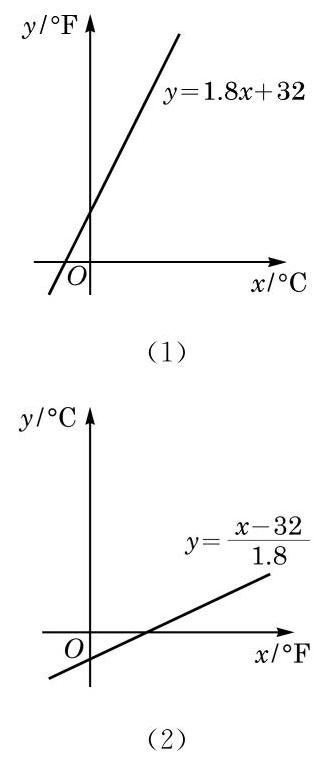
\includegraphics[max width=0.2\textwidth]{images/bo_d7fr3gc91nqc7381iccg_152_183_833_319_762_0.jpg}
\end{center}
\hspace*{3em} 

图 5-4-1

在进行摄氏度 \(\left( {{}^{ \circ  }\mathrm{C}}\right)\) 和华氏度 \(\left( {{}^{ \circ  }\mathrm{F}}\right)\) 两种温度单位换算时会发现, 有时选用相同的数据如表 5-4 所示, 但所建立的函数关系和作出的图像不同, 如图 5-4-1 所示.

表 5-4 华氏度与摄氏度的转换

\begin{center}
\adjustbox{max width=\textwidth}{
\begin{tabular}{|c|c|c|c|c|c|}
\hline
摄氏度/ \textdegree C & 0 & 20 & 35 & 100 & 115 \\
\cline{1-6}
华氏度/ \textdegree F & 32 & 68 & 95 & 212 & 239 \\
\cline{1-6}
\hline
\end{tabular}
}
\end{center}

这是为什么呢? 原来这两个函数所选取的自变量和函数值恰好相反. 看似完全不同的两个函数关系式和图像都正确反映了两种温度单位之间的转换关系, 前者将摄氏度转换为华氏度, 而后者恰好相反.

由于习惯上函数的自变量用 \(x\) 表示,在图像上作为点的横坐标,而函数值用 \(y\) 表示,在图像上作为点的纵坐标,因此 \(y = {1.8x} + {32}\) 的反函数通常写成 \(y = \frac{x - {32}}{1.8}\) .

定义 对于函数 \(y = f\left( x\right) ,x \in  D\) ,记其值域为 \(f\left( D\right)\) . 如果对 \(f\left( D\right)\) 中的任意给定的一个值 \(y\) ,在 \(D\) 中满足 \(f\left( x\right)  = y\) 的 \(x\) 值只有一个,那么由此得到的 \(x\) 关于 \(y\) 的函数叫做 \(y = f\left( x\right)\) , \(x \in  D\) 的反函数 (inverse function),记作 \(x = {f}^{-1}\left( y\right) ,y \in  f\left( D\right)\) .

\section*{}

由于自变量习惯上常用 \(x\) 表示,而函数值常用 \(y\) 表示,因此通常把该函数改写为

\[
y = {f}^{-1}\left( x\right) ,x \in  f\left( D\right) .
\]

例如,函数 \(y = {2x}\) 的反函数为 \(y = \frac{x}{2}\) ,函数 \(y = {3x} + 1\) 的反函数为 \(y = \frac{x - 1}{3}\) .

一个定义域为 \(D\) 的函数 \(y = f\left( x\right)\) 存在反函数,当且仅当对于其值域 \(f\left( D\right)\) 中的每一个值 \({y}_{0}\) ,在定义域 \(D\) 中仅存在一个 \({x}_{0}\) ,满足 \(f\left( {x}_{0}\right)  = {y}_{0}\) . 也就是说,如果函数 \(y = f\left( x\right)\) 在定义域 \(D\) 上不同的 \(x\) 处所取到的函数值也不相同,那么 \(y = f\left( x\right)\) 就存在反函数. 因此, 在定义域上的严格增函数或严格减函数均存在反函数.

从反函数的定义可知: 如果函数 \(y = f\left( x\right) ,x \in  D\) 存在反函数 \(y = {f}^{-1}\left( x\right) ,x \in  f\left( D\right)\) ,那么函数 \(y = {f}^{-1}\left( x\right) ,x \in  f\left( D\right)\) 的反函数就是 \(y = f\left( x\right) ,x \in  D\) . 也就是说, \(y = f\left( x\right)\) 及 \(y = {f}^{-1}\left( x\right)\) 是互为反函数的.

函数 \(y = {f}^{-1}\left( x\right)\) 的定义域就是 \(y = f\left( x\right)\) 的值域,函数 \(y = {f}^{-1}\left( x\right)\) 的值域就是函数 \(y = f\left( x\right)\) 的定义域.

例 1 若 \(f\left( x\right)  = {\log }_{3}x\) ,并设 \(y = {f}^{-1}\left( x\right)\) 是 \(y = f\left( x\right)\) 的反函数,求 \({f}^{-1}\left( 2\right) ,{f}^{-1}\left( a\right)\) .

解 设 \({f}^{-1}\left( 2\right)  = t\) ,根据反函数的定义,可得 \(f\left( t\right)  = 2\) ,即 \({\log }_{3}t = 2\) ,因此 \(t = 9\) ,即 \({f}^{-1}\left( 2\right)  = 9\) .

类似地,设 \({f}^{-1}\left( a\right)  = b\) ,可得 \(f\left( b\right)  = {\log }_{3}b = a\) ,即 \(b = {3}^{a}\) , 因此 \({f}^{-1}\left( a\right)  = {3}^{a}\) .

一般地,当 \(a > 0,a \neq  1\) 时,解关于 \(x\) 的方程 \(y = {\log }_{a}x\) ,得 \(x = {a}^{y}\) . 因此,当 \(a > 0,a \neq  1\) 时, \(y = {a}^{x}\) 与 \(y = {\log }_{a}x\) 互为反函数.

例 2 求下列函数的反函数:

(1) \(y = {4x} + 2\) ；

(2) \(y = {x}^{2} + 1,x \in  \left\lbrack  {1,3}\right\rbrack\) ；

(3) \(y = \frac{{3x} + 1}{{4x} + 2}\) .

解(1)该函数的值域为 \(\mathbf{R}\) . 解关于 \(x\) 的方程 \(y = {4x} + 2\) ， 得 \(x = \frac{y - 2}{4}\) . 因此,相应的反函数为 \(y = \frac{x - 2}{4}\) .

\HRule

在例 2(1) 中, 使得表达式 \(y = \frac{x - 2}{4}\) 有意义的 \(x\) 的范围已经是 \(y = {4x} + 2\) 的值域 \(\mathbf{R}\) 了, 因此此处反函数的定义域不必明显地写出. 例 2 (3)不注明反函数的定义域的理由类似.

\HRule

(2)该函数的值域为 \(\left\lbrack  {2,{10}}\right\rbrack\) .

在 \(x \in  \left\lbrack  {1,3}\right\rbrack  ,y \in  \left\lbrack  {2,{10}}\right\rbrack\) 的前提下,解关于 \(x\) 的方程 \(y = {x}^{2} + 1\) , 得 \(x = \sqrt{y - 1}\) . 因此,相应的反函数为 \(y = \sqrt{x - 1},x \in  \left\lbrack  {2,{10}}\right\rbrack\) .

(3)由 \(y = \frac{{3x} + 1}{{4x} + 2} = \frac{3}{4} - \frac{1}{{8x} + 4}\) 可知，该函数的值域为 \(\left\{  {y\left| {\;y \neq  \frac{3}{4}}\right. }\right\}\) .

在 \(x \neq   - \frac{1}{2},y \neq  \frac{3}{4}\) 的前提下,解关于 \(x\) 的方程 \(y = \frac{{3x} + 1}{{4x} + 2}\) , 得 \(x = \frac{1 - {2y}}{{4y} - 3}\) .

因此,相应的反函数为 \(y = \frac{1 - {2x}}{{4x} - 3}\) .

\section*{练习 5.4(1)}

1. 求函数 \(y = {x}^{2} + {2x},x \in  \lbrack 0, + \infty )\) 的反函数的定义域.

2. 求下列函数的反函数:

(1) \(y = {3x} + 2\) ； (2) \(y =  - \frac{3}{x}\) ；

(3) \(y = {x}^{2},x \in  ( - \infty ,0\rbrack\) ； (4) \(y = \sqrt{x} + 1\) .

3. 判断函数 \(y = \left\{  \begin{matrix} x, &  - 1 \leq  x \leq  0, \\  1 - x, & 0 < x < 1 \end{matrix}\right.\) 是否存在反函数. 若存在反函数,求出它的反函数; 若不存在反函数, 说明理由.

\section*{2 反函数的图像}

为了研究函数与其反函数的图像的特征, 我们需要一个如下的命题:

命题 在平面直角坐标系中,点 \(P\left( {a,b}\right)\) 与点 \({P}^{\prime }\left( {b,a}\right)\) 关于直线 \(y = x\) 成轴对称.

证明 当 \(a = b\) 时,点 \(P\) 与 \({P}^{\prime }\) 重合,且在直线 \(y = x\) 上,结论成立.

当 \(a \neq  b\) 时,点 \(P\) 与 \({P}^{\prime }\) 是不重合的两点,要证明它们关于直线 \(y = x\) 成轴对称,即证直线 \(y = x\) 是线段 \(P{P}^{\prime }\) 的垂直平分线.

线段 \(P{P}^{\prime }\) 的垂直平分线即点集 \(\left\{  {Q\left( {x,y}\right) \left| \right| {QP} \mid   = \left| {Q{P}^{\prime }}\right| }\right\}\) . 由

\section*{}

两点 \(\left( {{x}_{1},{y}_{1}}\right)\) 及 \(\left( {{x}_{2},{y}_{2}}\right)\) 之间的距离公式 \(\sqrt{{\left( {x}_{1} - {x}_{2}\right) }^{2} + {\left( {y}_{1} - {y}_{2}\right) }^{2}}\) , 该集合也可以表示为

\[
\left\{  {Q\left( {x,y}\right) \left| {\;\sqrt{{\left( x - a\right) }^{2} + {\left( y - b\right) }^{2}} = \sqrt{{\left( x - b\right) }^{2} + {\left( y - a\right) }^{2}}}\right. }\right\}  ,
\]

即 \(\{ Q\left( {x,y}\right)  \mid  {ax} + {by} = {bx} + {ay}\}\) .

因 \(a \neq  b\) ,故该集合为 \(\{ Q\left( {x,y}\right)  \mid  x = y\}\) .

所以,线段 \(P{P}^{\prime }\) 的垂直平分线是直线 \(y = x\) ,因而点 \(P\left( {a,b}\right)\) 与点 \({P}^{\prime }\left( {b,a}\right)\) 关于直线 \(y = x\) 对称.

作为指数函数和对数函数的图像关系在一般函数中的推广, 我们有

性质 互为反函数的两函数的图像关于直线 \(y = x\) 成轴对称.

证明 设函数 \(y = f\left( x\right) ,x \in  D\) 的反函数为 \(y = {f}^{-1}\left( x\right)\) , \(x \in  f\left( D\right)\) .

若 \(P\left( {a,b}\right)\) 为函数 \(y = f\left( x\right)\) 图像上任取的一点,则必有 \(a \in  D\) ,且 \(b = f\left( a\right)\) . 这样, \(b = f\left( a\right)  \in  f\left( D\right)\) ,且根据反函数的定义, \(a = {f}^{-1}\left( b\right)\) ,因此 \(P\left( {a,b}\right)\) 关于直线 \(y = x\) 的对称点 \({P}^{\prime }\left( {b,a}\right)\) 在函数 \(y = {f}^{-1}\left( x\right)\) 的图像上.

另一方面,因为 \(y = {f}^{-1}\left( x\right)\) 的反函数是 \(y = f\left( x\right)\) ,由上述, \(y = {f}^{-1}\left( x\right)\) 图像上任一点 \(Q\) 关于直线 \(y = x\) 的对称点 \({Q}^{\prime }\) 在函数 \(y = f\left( x\right)\) 的图像上.

综上所述,互为反函数的两函数的图像关于直线 \(y = x\) 成轴对称.

在求一个函数 \(y = f\left( x\right)\) 的反函数时,一般要经历下述三个步骤:求出反函数的定义域(即原来函数的值域)；解方程 \(y = f\left( x\right)\) ,求出 \(x\) 关于 \(y\) 的函数表达式; 再交换 \(x\) 与 \(y\) .

\begin{center}
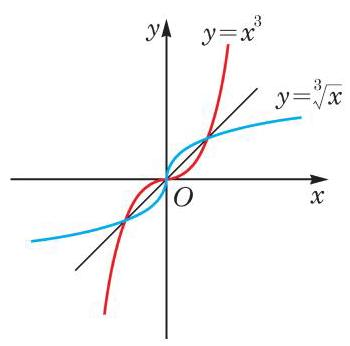
\includegraphics[max width=0.2\textwidth]{images/bo_d7fr3gc91nqc7381iccg_155_1127_1714_350_346_0.jpg}
\end{center}
\hspace*{3em} 

图 5-4-2

正是将 \(x\) 和 \(y\) 对换,即将点的横纵两个坐标作了对换,才导致了函数与其反函数的图像关于直线 \(y = x\) 对称.

例 3 求函数 \(y = {x}^{3}\) 的反函数,并在同一坐标系中作出函数 \(y = {x}^{3}\) 和它的反函数的图像.

解 \(y = {x}^{3}\) 的值域是 \(\mathbf{R}\) . 解关于 \(x\) 的方程 \(y = {x}^{3}\) ,得 \(x = \sqrt[3]{y}\) ,因此其反函数为 \(y = \sqrt[3]{x}\) .

同一坐标系中, \(y = {x}^{3}\) 的图像与 \(y = \sqrt[3]{x}\) 的图像如图 5-4-2

所示,它们关于直线 \(y = x\) 对称.

例 4 已知函数 \(y = {a}^{x} + b\) 的图像经过点 \(\left( {1,7}\right)\) ,而其反函数的图像经过点 \(\left( {4,0}\right)\) ,求实数 \(a\text{ 、 }b\) 的值.

解 由 \(y = {a}^{x} + b\) 的图像经过点 \(\left( {1,7}\right)\) ,可知 \(7 = {a}^{1} + b = \; a + b\) . 此外,其反函数的图像经过点 \(\left( {4,0}\right)\) ,也就是 \(y = {a}^{x} + b\) 的图像经过点 \(\left( {0,4}\right)\) ,故 \(4 = {a}^{0} + b = 1 + b\) .

由此解得 \(a\text{ 、 }b\) 的值分别为 4、3.

\section*{练习 5.4(2)}

1. 定义在 \(\mathbf{R}\) 上的偶函数存在反函数吗? 说明理由.

2. 下列各图中,存在反函数的函数 \(y = f\left( x\right)\) 的图像只可能是 ( )

\begin{center}
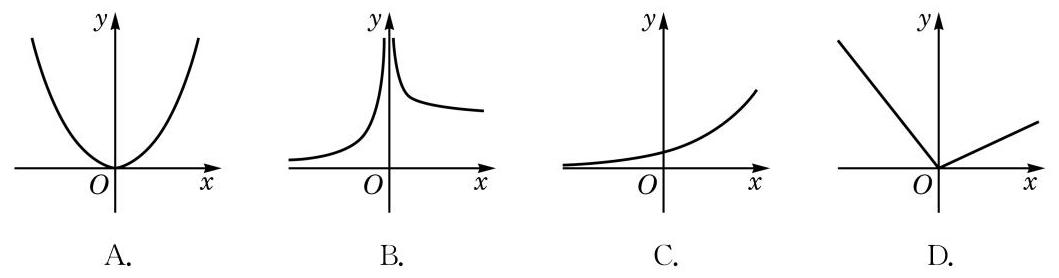
\includegraphics[max width=0.9\textwidth]{images/bo_d7fr3gc91nqc7381iccg_156_364_874_1059_278_0.jpg}
\end{center}
\hspace*{3em} 

(第 2 题)

3. 已知函数 \(y = f\left( x\right) ,x \in  D\) 存在反函数 \(y = {f}^{-1}\left( x\right) ,x \in  f\left( D\right)\) . 函数 \(y = f\left( {x + 1}\right)\) 与 \(y = {f}^{-1}\left( {x + 1}\right)\) 是否一定互为反函数? 说明理由.

\section*{习题 5.4}

\section*{A 组}

1. 已知函数 \(y = {x}^{2} - {4x} - 5,x \in  \left\lbrack  {1,3}\right\rbrack\) ,判断其是否存在反函数. 若存在,求出反函数; 若不存在, 说明理由.

2. 求下列函数的反函数:

(1) \(y =  - {x}^{3}\) ； (2) \(y = \frac{x}{x + 2}\) ； (3) \(y = {x}^{2} + 1,x \in  \left( {-\infty ,0}\right)\) .

3. 求下列函数的反函数:

(1) \(y = {10}^{x} + 1\) ； (2) \(y = {\log }_{2}\left( {x + 1}\right)\) ； (3) \(y = {\log }_{2}\left( {2x}\right)\) .

4. 已知 \(f\left( x\right)  = 1 - {\log }_{2}x\) ,设 \(y = {f}^{-1}\left( x\right)\) 是 \(y = f\left( x\right)\) 的反函数. 求 \({f}^{-1}\left( {-3}\right)\) 的值.

5. 已知函数 \(y = \frac{a}{x + 1}\) 的反函数的图像经过点 \(\left( {\frac{1}{2},1}\right)\) ,求实数 \(a\) 的值.

\section*{}

\section*{内容提要}

1. 函数的概念:

(1)设 \(D\) 是一个非空的数集，如果按照某种确定的对应关系 \(f\) ，使对集合 \(D\) 中任意给定的 \(x\) ，都有唯一的实数 \(y\) 与之对应，就称这个对应关系 \(f\) 为集合 \(D\) 上的一个函数.

(2)定义域和对应关系是函数的两个重要要素. 函数的值域由其定义域和对应关系决定. 两个函数的定义域和对应关系都相同(形式上未必相同)时，两个函数是相同的.

(3)函数的图像是表示函数性质的直观有力的工具。

2. 函数的性质:

(1)如果对定义域 \(D\) 中的任意给定的 \(x\) ，均有 \(- x \in  D\) ，并且 \(f\left( x\right)  = f\left( {-x}\right)\) ，那么称 \(y = f\left( x\right) ,x \in  D\) 是一个偶函数; 如果对定义域 \(D\) 中的任意给定的 \(x\) ,均有 \(- x \in  D\) ,并且 \(f\left( x\right)  =  - f\left( {-x}\right)\) ,那么称 \(y = f\left( x\right) ,x \in  D\) 是一个奇函数. 函数的奇偶性刻画了函数图像关于原点及 \(y\) 轴的对称性.

(2)对于定义在 \(D\) 上的函数 \(y = f\left( x\right)\) ，设区间 \(I\) 是 \(D\) 的子集. 对于区间 \(I\) 上的任意给定的两个自变量的值 \({x}_{1}\text{ 、 }{x}_{2}\) ,当 \({x}_{1} < {x}_{2}\) 时,如果总有 \(f\left( {x}_{1}\right)  < f\left( {x}_{2}\right) \left( {f\left( {x}_{1}\right)  \leq  }\right. \; \left. {f\left( {x}_{2}\right) }\right)\) ,就称函数 \(y = f\left( x\right)\) 在区间 \(I\) 上是严格增函数(增函数); 如果总有 \(f\left( {x}_{1}\right)  > f\left( {x}_{2}\right) \; \left( {f\left( {x}_{1}\right)  \geq  f\left( {x}_{2}\right) }\right)\) ,就称函数 \(y = f\left( x\right)\) 在区间 \(I\) 上是严格减函数(减函数). 这种单调性刻画了函数图像上升或下降的趋势.

(3)设函数 \(y = f\left( x\right)\) 在定义域内的 \({x}_{0}\) 处的函数值是 \(f\left( {x}_{0}\right)\) . 对于定义域内任意给定的 \(x\) ,如果不等式 \(f\left( x\right)  \geq  f\left( {x}_{0}\right)\) 都成立,那么 \(f\left( {x}_{0}\right)\) 叫做函数 \(y = f\left( x\right)\) 的最小值; 如果不等式 \(f\left( x\right)  \leq  f\left( {x}_{0}\right)\) 都成立，那么 \(f\left( {x}_{0}\right)\) 叫做函数 \(y = f\left( x\right)\) 的最大值. 最大值与最小值分别为函数图像的最高点与最低点的纵坐标.

3. 函数的应用:

(1)在建立函数关系时，需要注意其定义域.

(2)依靠函数 \(y = f\left( x\right)\) ，可以用动态的观点来考察方程 \(f\left( x\right)  = 0\) 的求解，以及不等式 \(f\left( x\right)  > 0\) 的求解.

(3)对于函数 \(y = f\left( x\right) ,x \in  D\) ,若存在 \(c \in  D\) ,且 \(f\left( c\right)  = 0\) ，则称 \(c\) 是函数 \(y = f\left( x\right) ,x \in  D\) 的一个零点. 零点是指函数图像与 \(x\) 轴交点的横坐标. 对于图像是连续曲线的函数，二分法是求近似零点的有效手段.

*4. 反函数:

(1)反函数来源于解关于 \(x\) 的方程 \(f\left( x\right)  = y\) 所得到的对应关系.

(2)如果函数 \(y = f\left( x\right)\) 在定义域 \(D\) 上不同的 \(x\) 处所取到的函数值也不相同，那么 \(y = f\left( x\right)\) 就存在反函数. 在定义域上严格单调的函数必存在反函数.

(3)函数 \(y = f\left( x\right)\) 的图像与其反函数 \(y = {f}^{-1}\left( x\right)\) 的图像关于直线 \(y = x\) 成轴对称.

\section*{复习题}

A 组

1. 求函数 \(y = \frac{1}{2 - x} + \sqrt{{x}^{2} - 1}\) 的定义域.

2. 判断下列函数 \(y = f\left( x\right)\) 的奇偶性,并说明理由:

(1) \(f\left( x\right)  = \left| {\frac{1}{2}x - 3}\right|  + \left| {\frac{1}{2}x + 3}\right|\) ;

(2) \(f\left( x\right)  = {x}^{3} + \frac{2}{x}\) ；

(3) \(f\left( x\right)  = {x}^{2},x \in  \left( {k,2}\right)\) (其中常数 \(k < 2\) ).

3. 已知 \(m\text{ 、 }n\) 是常数，而函数 \(y = \left( {m - 1}\right) {x}^{2} + {3x} + \left( {2 - n}\right)\) 为奇函数. 求 \(m\text{ 、 }n\) 的值.

4. 求函数 \(y = x + \frac{4}{x}\) 的单调区间.

5. 分别作出下列函数的大致图像, 并指出它们的单调区间:

(1) \(y = \left| {{x}^{2} - {4x}}\right|\) ;

(2) \(y = 2\left| x\right|  - 3\) .

6. 已知二次函数 \(y = f\left( x\right)\) ,其中 \(f\left( x\right)  = a{x}^{2} - {2ax} + 3 - a\left( {a > 0}\right)\) . 比较 \(f\left( {-1}\right)\) 和 \(f\left( 2\right)\) 的大小.

7. 已知 \(k\) 是常数，设 \(\alpha\) 、 \(\beta\) 是二次方程 \({x}^{2} - {2kx} + k + {20} = 0\) 的两个实根. 问:当 \(k\) 为何值时, \({\left( \alpha  + 1\right) }^{2} + {\left( \beta  + 1\right) }^{2}\) 取到最小值?

8. 邮局规定:当邮件质量不超过 \({100}\mathrm{\;g}\) 时，每 \({20}\mathrm{\;g}\) 邮费 0.8 元，且不足 \({20}\mathrm{\;g}\) 时按 \({20}\mathrm{\;g}\) 计算; 超过 \({100}\mathrm{\;g}\) 时,超过 \({100}\mathrm{\;g}\) 的部分按每 \({100}\mathrm{\;g}\) 邮费 2 元计算,且不足 \({100}\mathrm{\;g}\) 按 \({100}\mathrm{\;g}\) 计算; 同时规定邮件总质量不得超过 2000 g. 请写出邮费关于邮件质量的函数表达式, 并计算 \({50}\mathrm{\;g}\) 和 \({500}\mathrm{\;g}\) 的邮件分别收多少邮费.

9. 若函数 \(y = \left( {{a}^{2} + {4a} - 5}\right) {x}^{2} - 4\left( {a - 1}\right) x + 3\) 的图像都在 \(x\) 轴上方 (不含 \(x\) 轴),求实数 \(a\) 的取值范围.

\section*{B 组}

1. 已知 \(y = f\left( x\right)\) 是奇函数,其定义域为 \(\mathbf{R}\) ; 而 \(y = g\left( x\right)\) 是偶函数,其定义域为 \(D\) .

\section*{}

判断函数 \(y = f\left( x\right) g\left( x\right)\) 的奇偶性,并说明理由.

2. 设函数 \(y = {x}^{2} + {10x} - a + 3\) ,当 \(x \in  \lbrack  - 2, + \infty )\) 时，其函数值恒大于等于零. 求实数 \(a\) 的取值范围.

3. 已知函数 \(y =  - {x}^{2} + {2ax} + 1 - a,x \in  \left\lbrack  {0,1}\right\rbrack\) 的最大值为 2 . 求实数 \(a\) 的值.

4. 设 \(f\left( x\right)  = {x}^{2} + {ax} + 1\) . 若对任意给定的实数 \(x,f\left( {2 + x}\right)  = f\left( {2 - x}\right)\) 恒成立,求实数 \(a\) 的值.

5. 已知 \(y = f\left( x\right)\) 是定义在 \(\left( {-1,1}\right)\) 上的奇函数,在区间 \(\lbrack 0,1)\) 上是严格减函数,且 \(f\left( {1 - a}\right)  + f\left( {1 - {a}^{2}}\right)  < 0\) . 求实数 \(a\) 的取值范围.

6. 已知 \(f\left( x\right)  = 2 - {x}^{2}\) 及 \(g\left( x\right)  = x\) . 定义 \(h\left( x\right)\) 如下: 当 \(f\left( x\right)  \geq  g\left( x\right)\) 时, \(h\left( x\right)  = g\left( x\right)\) ; 而当 \(f\left( x\right)  < g\left( x\right)\) 时, \(h\left( x\right)  = f\left( x\right)\) . 求函数 \(y = h\left( x\right)\) 的最大值.

\section*{拓展与思考}

1. 试讨论函数 \(y = \frac{x}{1 - {x}^{2}}\) 的单调性.

2. 作出函数 \(y = {\left( {x}^{2} - 1\right) }^{2} - 1\) 的大致图像,写出它的单调区间,并证明你的结论.

3. 已知函数 \(y = f\left( x\right)\) 为偶函数, \(y = g\left( x\right)\) 为奇函数,且 \(f\left( x\right)  + g\left( x\right)  = {x}^{2} + 2\left| {x - 1}\right|  + 3\) . 求 \(y = f\left( x\right)\) 及 \(y = g\left( x\right)\) 的表达式.

*4. 设函数 \(y = f\left( x\right) ,x \in  \mathbf{R}\) 的反函数是 \(y = {f}^{-1}\left( x\right)\) .

(1)如果 \(y = f\left( x\right)\) 是奇函数，那么 \(y = {f}^{-1}\left( x\right)\) 的奇偶性如何?

(2)如果 \(y = f\left( x\right)\) 在定义域上是严格增函数，那么 \(y = {f}^{-1}\left( x\right)\) 的单调性如何？

\section*{后 记}

本套高中数学教材根据教育部颁布的《普通高中数学课程标准 (2017 年版 2020 年修订)》编写并经国家教材委员会专家委员会审核通过.

本教材是由设在复旦大学和华东师范大学的两个上海市数学教育教学研究基地(上海高校“立德树人”人文社会科学重点研究基地)联合主持编写的. 编写工作依据高中数学课程标准的具体要求，努力符合教育规律和高中学生的认知规律，结合上海城市发展定位和课程改革基础，并力求充分体现特色. 希望我们的这一努力能经得起实践和时间的检验, 对扎实推进数学的基础教育发挥积极的作用.

本册教材是必修第一册, 共为五章, 各章编写人员分别为

王伟叶、傅吉祥(第 1 章)

王春明、王志强(第 2 章)

潘奋、吴泉水、高卫国(第 3 章、第 4 章)

王伟叶、邱维元(第 5 章)

上海市中小学(幼儿园)课程改革委员会专家工作委员会、上海市教育委员会教学研究室全程组织、指导和协调了教材编写工作. 在编写过程中，两个基地所在单位给予了大力支持，基地的全体同志积极参与相关的调研、讨论及评阅工作，发挥了重要的作用. 上海市不少中学也热情地参与了有关的调研及讨论工作. 有限公司不但是编辑出版单位，而且自始至终全面介入了编写工作. 我们对所有这些单位和相关人员的参与、支持和鼓励表示衷心感谢.

限于编写者的水平, 也由于新编教材尚缺乏教学实践的检验, 不妥及疏漏之处在所难免，恳请广大师生及读者不吝赐教. 宝贵意见请通过邮箱 gaozhongshuxue@seph.com.cn 反馈, 不胜感激.

2020 年 7 月



\section*{SHUXUE 普通高中教科书 数学 必修}

第 一 册

\begin{center}
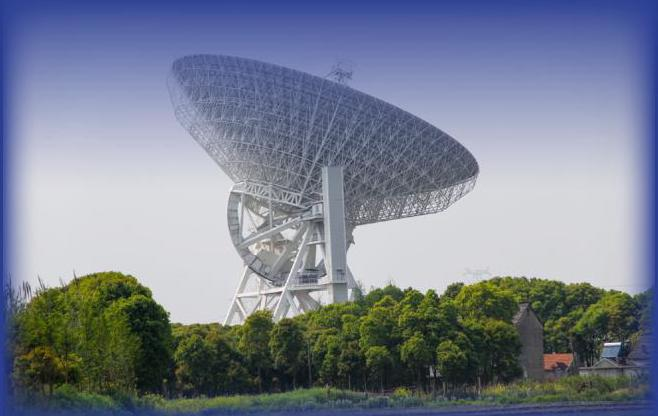
\includegraphics[max width=0.5\textwidth]{images/bo_d7fr3gc91nqc7381iccg_161_493_1026_658_416_0.jpg}
\end{center}
\hspace*{3em} 

2024 蛰伏

精进

\section*{IATEX 实用功能简介}

整理错题、积累典型题、记录教学心得、整理解题笔记必备工具

编写试卷讲义、制作课件、出版校本教材的不二选择

数学老师的新一代生产力工具

向每一个选择长期主义的老师致敬

\section*{目录}

一、IATEX 是什么？软件的渊源、使用人群和 IATEX 生态 2

1.1 软件渊源 2

1.2 使用人群 2

1.3 IATEX 生态 2

二、软件功能简介 3

2.1 编辑数学公式高效、规范、稳定 3

2.2 编辑试卷、讲义、校本教材自动化程度高 4

2.3 画图高效、美观、方便修改与正文浑然一体 4

2.4 试题、讲义、校本教材效果展示 5

试卷 5

讲义 8

校本教材 9

知 幻灯片 10

2.5 数学作图方便、精准、美观与文档浑然一体 12

函数图 12

知立体图 12

统计图 12

知圆锥曲线图 13

知其他平面图 13

4 其它图形 14

知三视图 14

4 与文档浑然一体 16

三、课程简介与学习流程 17

附件二:公式效果 18

\section*{面向中学数学教师的 IATEX 培训课程手册}

\section*{一、 IATEX 是什么？软件的渊源、使用人群和 IATEX 生态}

\section*{1.1 软件渊源}

图灵奖得主高德纳教授在修订他的《计算机程序设计的艺术》(这本书的学界地位与《几何原本》、《相对论》、《量子力学》比肩而立) 第二卷时，因不满出版社的排版质量而自己设计了一个新的排版系统 TEX，这就是 LaTeX 的前身，经过兰伯特、美国数学学会以及其他的行业大咖不断维护更新, 形成了今天的 LATEX, 广泛应用于理工科文档编辑排版, 被誉为排版之王, 甚至很多杂志也要求用 LATEX 排版.

\section*{1.2 使用人群}

IATEX 以其在编辑数学公式方面无可比拟的优势而闻名于世, 目前在国外家喻户晓，在国内的使用者主要是大学理工科教授、研究所、科技企业、 出版社. 最早就是由中科院吴凌云等教授汉化软件并在国内推广的, 现在很多名校的理工科的研究生 (尤其是数学专业的研究生) 的毕业论文都必须使用IATEX 完成。

\section*{1.3 IATEX 生态}

IATEX 已经作为行业标准, 广泛应用于和公式编辑相关的大多数场景, 越来越多的公司提供相关服务，比如 mathpix、腾讯云、有道云都可以将图片版的数学公式转化为 \(\mathrm{I}\) ATEX,可以大大提高公式的输入效率. 越来越多的出版社包括科学出版社、中科大出版社、浙江大学出版社、清华大学出版社支持 IATEX 书稿出版.

随着中学教师的学历的不断提升，电脑的普及，信息化能力的提升，很多教师都萌生了整理自己的教学成果，教学资料的想法，以前苦于没有良好的工具, 自从 LATEX 被引进中学老师圈, 越来越多的中学老师使用 LATEX 编辑整理教案、讲义、试卷、画图、校本教材，使用 IATEX 在中学已经蔚然成风.

\section*{二、软件功能简介}

\section*{2.1 编辑数学公式高效、规范、稳定}

IATEX 输入数学公式全部通过键盘的, 而不需要像公式编辑器那样通过鼠标点击来回切换插入公式，减少麻烦，另外 LATEX 的符号更加全面，老师们不会因为找不到符号而苦恼.

除了编辑效率高, 还有规范、稳定的优势. LATEX 编辑的公式与文本格式统一, 大小字号也可以统一调整, 也可以任意复制粘贴, 在任意电脑上播放, 永不变形、不错位、不乱码, 受到老师们的一致喜爱. 以下为效果:

\[
f\left( x\right)  = \left\{  \begin{array}{ll} {x}^{2} - {2x} + 3, & x \leq  1, \\  x - 2, & x > 1. \end{array}\right. \;\left\{  \begin{array}{l} \widehat{b} = \frac{\mathop{\sum }\limits_{{i = 1}}^{n}\left( {{x}_{i} - \bar{x}}\right) \left( {{y}_{i} - \bar{y}}\right) }{\mathop{\sum }\limits_{{i = 1}}^{n}{\left( {x}_{i} - \bar{x}\right) }^{2}} = \frac{\mathop{\sum }\limits_{{i = 1}}^{n}{x}_{i}{y}_{i} - n\bar{x}\bar{y}}{\mathop{\sum }\limits_{{i = 1}}^{n}{x}_{i}^{2} - n{\bar{x}}^{2}} \\  \widehat{a} = \bar{y} - \widehat{b}\bar{x} \end{array}\right.
\]

\[
\mathop{\sum }\limits_{{i = 1}}^{n}\left( {{x}_{i} - \bar{x}}\right) \left( {{y}_{i} - \bar{y}}\right)
\]

\[
= \left( {{x}_{1} - \bar{x}}\right) \left( {{y}_{1} - \bar{y}}\right)  + \left( {{x}_{2} - \bar{x}}\right) \left( {{y}_{2} - \bar{y}}\right)  + \cdots \left( {{x}_{n} - \bar{x}}\right) \left( {{y}_{n} - \bar{y}}\right)
\]

\[
= \left( {{x}_{1}{y}_{1} - {x}_{1}\bar{y} - \bar{x}{y}_{1} + \bar{x}\bar{y}}\right)  + \left( {{x}_{2}{y}_{2} - {x}_{2}\bar{y} - \bar{x}{y}_{2} + \bar{x}\bar{y} + \cdots  + \left( {{x}_{n}{y}_{n} - {x}_{n}\bar{y} - \bar{x}{y}_{n} + \bar{x}\bar{y}}\right) }\right.
\]

\[
= \left( {{x}_{1}{y}_{1} + {x}_{2}{y}_{2} + \cdots  + {x}_{n}{y}_{n}}\right)  - \left( {{x}_{1} + {x}_{2} + \cdots  + {x}_{n}}\right) \bar{y} - \bar{x}\left( {{y}_{1} + {y}_{2} + \cdots  + {y}_{n}}\right)  + n\bar{x}\bar{y}
\]

\[
= \mathop{\sum }\limits_{{i = 1}}^{n}{x}_{i}{y}_{i} - \left( {\mathop{\sum }\limits_{{i = 1}}^{n}{x}_{i}}\right) \bar{y} - \bar{x}\left( {\mathop{\sum }\limits_{{i = 1}}^{n}{y}_{i}}\right)  + n\bar{x}\bar{y}
\]

\[
= \mathop{\sum }\limits_{{i = 1}}^{n}{x}_{i}{y}_{i} - n\bar{x} \cdot  \bar{y} - \bar{x} \cdot  n\bar{y} + n\bar{x}\bar{y}
\]

\[
= \mathop{\sum }\limits_{{i = 1}}^{n}{x}_{i}{y}_{i} - n\bar{x}\bar{y}
\]

很多老师在准备公开课时, 由于公式编辑器的效率低甚至符号不全, 大多选择拼凑、修改一些课件，而这些课件的公式格式混乱、不规范，修改的时间比重新输入都要长,让老师们感到精疲力尽. LATEX 的编辑效率高、规范、稳定, 公式直接编辑就行了, 让老师把主要精力放到作课的思路上, 节约老师大量时间和心理成本.

\section*{2.2 编辑试卷、讲义、校本教材自动化程度高}

IATEX 自动化程度高最重要的体现方面是可以一键控制是否显示试题的答案、分析、详细解析, 从而得到学生版和教师版, 也可以单独得到答案, 这个过程不需要逐一的剪切、粘贴答案. 另外也可以实现:

1. 试题的来源、难度等试题标识能够一键控制是否显示;

2. 能够一键设置 A4 纸、A3 纸，单栏、双栏、多栏，无需过多调整；

3. 题号自动生成、对齐，调换顺序不用手动编号，不用担心答案不匹配；

4. 试题后的距离, 可一键控制是否显示, 可根据需要给学生留作答空间;

5. 选择题的选项可以自动排版, 会根据选项的长短自动确定一行排四个、 两个或一个选项, 选择题括号生成、自动右对齐;

6. 解答题的序号可以一键全部设置为罗马数字或阿拉伯数字.

这些自动化的设计极大地提高了教师整理试题、编写文档的效率，方便老师整理自己的讲义, 给学生更有针对性的出题, 布置作业. 还可以给讲义设置很多漂亮的文档结构, 也可以根据实际需要定制各种各样的功能.

\section*{2.3 画图高效、美观、方便修改与正文浑然一体}

数学画图是中学老师们遇到的另一个难题, 虽然也有几何画板、GeoGe-bra 等诸多软件可以画图, 但是也会存在一些问题, 比如:

1. 很多图画得慢, 不精确, 甚至画不出来. 如: 立体图、程序框图等;

2. 在图中输入数学公式比较麻烦, 图中文字的字体、大小也不容易统一;

3. 清晰度不高. 将其他软件制作的图插入文档，清晰的度会降低.

4. 细节调整比较麻烦, 后期修改不方便. 比如: 调整坐标轴的箭头, 坐标的位置等比较麻烦, 如果后期修改之前图中的错误, 几乎需要重做.

IATEX 画图可以完美解决这些问题, 不仅仅前期画图方便, 字体字号可以统一调整, 图中可以插入任意公式, 自由编辑. 在可修改性和复用性方面更是无可比拟. 比如题干中画好的图, 在解析中仍然可以在画好的图上进行编辑.

接下来我们来看具体效果.

\section*{2.4 试题、讲义、校本教材效果展示}

\section*{试卷}

按秘密事项管理 \ding{72} 启用前

\section*{2024 全国新课标 I 卷}

\section*{一、选择题: 本大题共 8 小题, 每小题 5 分, 共 40 分. 在每小题给出的四个选项中, 只有 一项是符合题目要求的.}

1. 已知集合 \(A = \left\{  {x \mid   - 5 < {x}^{3} < 5}\right\}  ,B = \{  - 3, - 1,0,2,3\}\) ,则 \(A \cap  B =\) ( )

A. \(\{  - 1,0\}\) B. \(\{ 2,3\}\) C. \(\{  - 3, - 1,0\}\) D. \(\{  - 1,0,2\}\)

2. 若 \(\frac{z}{z - 1} = 1 + \mathrm{i}\) ,则 \(z =\) ( )

A. \(- 1 - \mathrm{i}\) B. \(- 1 + \mathrm{i}\) C. \(1 - \mathrm{i}\) D. \(1 + \mathrm{i}\)

3. 已知向量 \(\mathbf{a} = \left( {0,1}\right) ,\mathbf{b} = \left( {2,x}\right)\) ,若 \(\mathbf{b} \bot  \left( {\mathbf{b} - 4\mathbf{a}}\right)\) ,则 \(x =\) ( )

A. -2 B. -1 C. 1 D. 2

4. 已知 \(\cos \left( {\alpha  + \beta }\right)  = m,\tan \alpha \tan \beta  = 2\) ,则 \(\cos \left( {\alpha  - \beta }\right)  =\) ( )

A. \(- {3m}\) B. \(- \frac{m}{3}\) C. \(\frac{m}{3}\) D. \({3m}\)

5. 已知圆柱和圆锥的底面半径相等，侧面积相等，且它们的高均为 \(\sqrt{3}\) ，则圆锥的体积为 ( )

A. \(2\sqrt{3}\pi\) B. \(3\sqrt{3}\pi\) C. \(6\sqrt{3}\pi\) D. \(9\sqrt{3}\pi\)

6. 已知函数 \(f\left( x\right)  = \left\{  \begin{array}{ll}  - {x}^{2} - {2ax} - a, & x < 0 \\  {\mathrm{e}}^{x} + \ln \left( {x + 1}\right) , & x \geq  0 \end{array}\right.\) 在 \(\mathbf{R}\) 上单调递增,则 \(a\) 的取值范围是 ( )

A. \(( - \infty ,0\rbrack\) B. \(\left\lbrack  {-1,0}\right\rbrack\) C. \(\left\lbrack  {-1,1}\right\rbrack\) D. \(\lbrack 0, + \infty )\)

7. 当 \(x \in  \left\lbrack  {0,{2\pi }}\right\rbrack\) 时,曲线 \(y = \sin x\) 与 \(y = 2\sin \left( {{3x} - \frac{\pi }{6}}\right)\) 的交点个数为 ( )

A. 3 B. 4 C. 6 D. 8

8. 已知函数为 \(f\left( x\right)\) 的定义域为 \(\mathbf{R},f\left( x\right)  > f\left( {x - 1}\right)  + f\left( {x - 2}\right)\) ,且当 \(x < 3\) 时, \(f\left( x\right)  = x\) , 则下列结论中一定正确的是 ( )

A. \(f\left( {10}\right)  > {100}\) B. \(f\left( {20}\right)  > {1000}\) C. \(f\left( {10}\right)  < {1000}\) D. \(f\left( {20}\right)  < {10000}\)

\section*{二、选择题: 本题共 3 小题, 每小题 6 分, 共 18 分. 在每小题给出的选项中, 有多项符合 题目要求. 全部选对的得 6 分, 部分选对的得部分分, 有选错的得 0 分.}

9. 多选题:随着”一带一路”国际合作的深入，某茶叶种植区多措并举推动茶叶出口. 为了解推动出口后的亩收入 (单位: 万元) 情况, 从该种植区抽取样本, 得到推动出口后亩收入的样本均值 \(\bar{x} = {2.1}\) ,样本方差 \({s}^{2} = {0.01}\) ,已知该种植区以往的亩收入 \(X\) 服从正态分布 \(N\left( {{1.8},{0.1}^{2}}\right)\) . 假设推动出口后的亩收入 \(Y\) 服从正态分布 \(N\left( {\bar{x},{s}^{2}}\right)\) ,则 (若随机变量 \(Z\) 服从正态分布 \(N\left( {\mu ,{\sigma }^{2}}\right)\) ,则 \(P\left( {Z < \mu  + \sigma }\right)  \approx  {0.8413}\) ) ( )

A. \(P\left( {X > 2}\right)  > {0.2}\) B. \(P\left( {X > 2}\right)  < {0.5}\) C. \(P\left( {Y > 2}\right)  > {0.5}\) D. \(P\left( {Y > 2}\right)  < {0.8}\) 10. 多选题,设函数 \(f\left( x\right)  = {\left( x - 1\right) }^{2}\left( {x - 4}\right)\) ,则 ( )

A. \(x = 3\) 是 \(f\left( x\right)\) 的极小值点 B. 当 \(0 < x < 1\) 时, \(f\left( x\right)  < f\left( {x}^{2}\right)\)

C. 当 \(1 < x < 2\) 时, \(- 4 < f\left( {{2x} - 1}\right)  < 0\) D. 当 \(- 1 < x < 0\) 时, \(f\left( {2 - x}\right)  > f\left( x\right)\)

\begin{center}
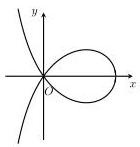
\includegraphics[max width=0.2\textwidth]{images/bo_d7fr3gc91nqc7381iccg_167_1323_722_140_147_0.jpg}
\end{center}
\hspace*{3em} 

11. (多选题) 设计一条美丽的丝带,其造型 \(\smallsetminus   \text{ ○ }\) 可以看作图中的曲线 \(C\) 的一部分,已知 \(C\) 过坐标原点 \(O\) ,且 \(C\) 上的点满足横坐标大于 -2,到点 \(F\left( {2,0}\right)\) 的距离与到定直线 \(x = a\left( {a < 0}\right)\) 的距离之积为 4 , 则 ( )

A. \(a =  - 2\)

B. 点 \(\left( {2\sqrt{2},0}\right)\) 在 \(C\) 上

C. \(C\) 在第一象限的点的纵坐标的最大值为 1

D. 当点 \(\left( {{x}_{0},{y}_{0}}\right)\) 在 \(C\) 上时, \({y}_{0} \leq  \frac{4}{{x}_{0} + 2}\)

\section*{三、填空题:本大题共 3 小题，每小题 5 分，共 15 分.}

12. 设双曲线 \(C : \frac{{x}^{2}}{{a}^{2}} - \frac{{y}^{2}}{{b}^{2}} = 1\left( {a > 0,b > 0}\right)\) 的左右焦点分别为 \({F}_{1},{F}_{2}\) ,过 \({F}_{2}\) 作平行于 \(y\) 轴的直线交 \(C\) 于 \(A,B\) 两点,若 \(\left| {{F}_{1}A}\right|  = {13},\left| {AB}\right|  = {10}\) ,则 \(C\) 的离心率为

13. 若曲线 \(y = {\mathrm{e}}^{x} + x\) 在点 \(\left( {0,1}\right)\) 处的切线也是曲线 \(y = \ln \left( {x + 1}\right)  + a\) 的切线,则 \(a =\)

2024 全国新课标 I 卷 第 1 页 共 2 页

14. 甲、乙两人各有四张卡片，每张卡片上标有一个数字，甲的卡片上分别标有数字 1,3,5,7,乙的卡片上分别标有数字2,4,6,8. 两人进行四轮比赛,在每轮比赛中,两人各自从自己持有的卡片中随机选一张，并比较所选卡片上数字的大小，数字大的人得 1 分, 数字小的人得 0 分, 然后各自弃置此轮所选的卡片 (弃置的卡片在此后的轮次中不能使用). 则四轮比赛比赛后, 甲的总得分不小于 2 的概率为

\section*{四、解答题:本大题共 5 小题, 共 77 分. 解答应写出必要的文字说明、证明过程或演算 步骤.}

15. 记 \(\bigtriangleup {ABC}\) 的内角 \(A,B,C\) 的对边分别为 \(a,b,c\) ,已知 \(\sin C = \sqrt{2}\cos B,{a}^{2} + {b}^{2} - {c}^{2} = \; \sqrt{2}{ab}\) .

( 1 ) 求 \(B\) ;

(2) 若 \(\bigtriangleup {ABC}\) 的面积为 \(3 + \sqrt{3}\) ,求 \(c\) .

16. 已知 \(A\left( {0,3}\right)\) 和 \(P\left( {3,\frac{3}{2}}\right)\) 为椭圆 \(C : \frac{{x}^{2}}{{a}^{2}} + \frac{{y}^{2}}{{b}^{2}} = 1\left( {a > b > 0}\right)\) 上两点.

( 1 ) 求 \(C\) 的离心率;

( 2 ) 若过 \(P\) 的直线 \(l\) 交 \(C\) 于另一点 \(B\) ,且 \(\bigtriangleup {ABP}\) 的面积为 9,求 \(l\) 的方程.

17. 如图,四棱锥 \(P - {ABCD}\) 中, \({PA} \bot\) 底面 \({ABCD},{PA} = {AC} = 2,{BC} = 1,{AB} = \sqrt{3}\) .

( 1 ) 若 \({AD} \bot  {PB}\) ,证明: \({AD}//\) 平面 \({PBC}\) ;

( 2 ) 若 \({AD} \bot  {DC}\) ,且二面角 \(A - {CP} - D\) 的正弦值为 \(\frac{\sqrt{42}}{7}\) ,求 \({AD}\) .

\begin{center}
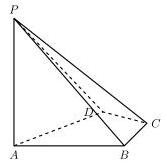
\includegraphics[max width=0.2\textwidth]{images/bo_d7fr3gc91nqc7381iccg_167_687_1911_167_163_0.jpg}
\end{center}
\hspace*{3em} 

18. 已知函数 \(f\left( x\right)  = \ln \frac{x}{2 - x} + {ax} + b{\left( x - 1\right) }^{3}\)

( 1 ) 若 \(b = 0\) ,且 \({f}^{\prime }\left( x\right)  \geq  0\) ,求 \(a\) 的最小值;

( 2 ) 证明: 曲线 \(y = f\left( x\right)\) 是中心对称图形;

( 3 ) 若 \(f\left( x\right)  >  - 2\) ,当且仅当 \(1 < x < 2\) ,求 \(b\) 的取值范围.

19. 设 \(m\) 为正整数,数列 \({a}_{1},{a}_{2},\cdots ,{a}_{{4m} + 2}\) 是公差不为 0 的等差数列,若从中删去两项 \({a}_{i}\) 和 \({a}_{j}\left( {i < j}\right)\) 后剩余的 \({4m}\) 项可被平均分为 \(m\) 组,且每组的 4 个数都能构成等差数列,则称数列 \({a}_{1},{a}_{2},\cdots ,{a}_{{4m} + 2}\) 是 \(\left( {i,j}\right)\) - 可分数列.

(1)写出所有的 \(\left( {i,j}\right) ,1 \leq  i < j \leq  6\) ,使数列 \({a}_{1},{a}_{2},\cdots ,{a}_{6}\left( {i,j}\right)\) - 可分数列;

( 2 ) 当 \(m \geq  3\) 时,证明: 数列 \({a}_{1},{a}_{2},\cdots ,{a}_{{4m} + 2}\) 是 \(\left( {2,{13}}\right)  -\) 可分数列;

( 3 ) 从 \(1,2,\cdots ,{4m} + 2\) 中一次任取两个数 \(i\) 和 \(j\left( {i < j}\right)\) ,记数列 \({a}_{1},{a}_{2},\cdots ,{a}_{{4m} + 2}\) 是 \(\left( {i,j}\right)\) - 可分数列的概率为 \({P}_{m}\) ,证明 \({P}_{m} > \frac{1}{8}\) .

按秘密事项管理 \ding{72} 启用前

\section*{2024 全国新课标 I 卷}

一、选择题: 本大题共 8 小题, 每小题 5 分, 共 40 分. 在每小题给出的四个选项中, 只有一项是符合题目要求的.

1. 已知集合 \(A = \left\{  {x \mid   - 5 < {x}^{3} < 5}\right\}  ,B = \{  - 3, - 1,0,2,3\}\) ,则 \(A \cap  B =\)

A. \(\{  - 1,0\}\) B. \(\{ 2,3\}\) C. \(\{  - 3, - 1,0\}\) D. \(\{  - 1,0,2\}\)

2. 若 \(\frac{z}{z - 1} = 1 + \mathrm{i}\) ,则 \(z =\) ( )

A. \(- 1 - \mathrm{i}\) B. \(- 1 + \mathrm{i}\) C. \(1 - \mathrm{i}\) D. \(1 + \mathrm{i}\)

3. 已知向量 \(\mathbf{a} = \left( {0,1}\right) ,\mathbf{b} = \left( {2,x}\right)\) ,若 \(\mathbf{b} \bot  \left( {\mathbf{b} - 4\mathbf{a}}\right)\) ,则 \(x =\) ( )

A. -2 B. -1 C. 1 D. 2

4. 已知 \(\cos \left( {\alpha  + \beta }\right)  = m,\tan \alpha \tan \beta  = 2\) ,则 \(\cos \left( {\alpha  - \beta }\right)  =\) ( )

A. \(- {3m}\) B. \(- \frac{m}{3}\) C. \(\frac{m}{3}\) D. \({3m}\)

5. 已知圆柱和圆锥的底面半径相等，侧面积相等，且它们的高均为 \(\sqrt{3}\) ，则圆锥的体积为 ( )

A. \(2\sqrt{3}\pi\) B. \(3\sqrt{3}\pi\) C. \(6\sqrt{3}\pi\) D. \(9\sqrt{3}\pi\)

6. 已知函数 \(f\left( x\right)  = \left\{  \begin{array}{ll}  - {x}^{2} - {2ax} - a, & x < 0 \\  {\mathrm{e}}^{x} + \ln \left( {x + 1}\right) , & x \geq  0 \end{array}\right.\) 在 \(\mathbf{R}\) 上单调递增,则 \(a\) 的取值范围是 ( A. \(( - \infty ,0\rbrack\) B. \(\left\lbrack  {-1,0}\right\rbrack\) C. \(\left\lbrack  {-1,1}\right\rbrack\) D. \(\lbrack 0, + \infty )\)

7. 当 \(x \in  \left\lbrack  {0,{2\pi }}\right\rbrack\) 时,曲线 \(y = \sin x\) 与 \(y = 2\sin \left( {{3x} - \frac{\pi }{6}}\right)\) 的交点个数为

A. 3 B. 4 C. 6 D. 8

关注【觅宁参考】即可联系作者，获取无水印有答案版本，也可以学公式编辑与排版

关注微信公众号:宽宁参考

三、填空题:本大题共 3 小题，每小题 5 分，共 15 分.

12. 设双曲线 \(C : \frac{{x}^{2}}{{a}^{2}} - \frac{{y}^{2}}{{b}^{2}} = 1\left( {a > 0,b > 0}\right)\) 的左右焦点分别为 \({F}_{1},{F}_{2}\) ,过 \({F}_{2}\) 作平行于 \(y\) 轴的直线交 \(C\) 于 \(A,B\) 两点,若 \(\left| {{F}_{1}A}\right|  = {13},\left| {AB}\right|  = {10}\) ,则 \(C\) 的离心率为

13. 若曲线 \(y = {\mathrm{e}}^{x} + x\) 在点 \(\left( {0,1}\right)\) 处的切线也是曲线 \(y = \ln \left( {x + 1}\right)  + a\) 的切线,则 \(a =\) \_\_\_\_\_.

14. 甲、乙两人各有四张卡片，每张卡片上标有一个数字，甲的卡片上分别标有数字 1,3,5,7,乙的卡片上分别标有数字2,4,6,8. 两人进行四轮比赛,在每轮比赛中,两人各自从自己持有的卡片中随机选一张, 并比较所选卡片上数字的大小, 数字大的人得 1 分, 数字小的人得 0 分, 然后各自弃置此轮所选的卡片 (弃置的卡片在此后的轮次中不能使用). 则四轮比赛比赛后, 甲的总得分不小于 2 的概率为 .

四、解答题:本大题共 5 小题, 共 77 分. 解答应写出必要的文字说明、证明过程或演算步骤.

15. 记 \(\bigtriangleup {ABC}\) 的内角 \(A,B,C\) 的对边分别为 \(a,b,c\) ,已知 \(\sin C = \sqrt{2}\cos B,{a}^{2} + {b}^{2} - {c}^{2} = \; \sqrt{2}{ab}\) .

( 1 ) 求 \(B\) ;

(2 ) 若 \(\bigtriangleup {ABC}\) 的面积为 \(3 + \sqrt{3}\) ,求 \(c\) .

16. 已知 \(A\left( {0,3}\right)\) 和 \(P\left( {3,\frac{3}{2}}\right)\) 为椭圆 \(C : \frac{{x}^{2}}{{a}^{2}} + \frac{{y}^{2}}{{b}^{2}} = 1\left( {a > b > 0}\right)\) 上两点.

(1)求 \(C\) 的离心率；

(2)若过 \(P\) 的直线 \(l\) 交 \(C\) 于另一点 \(B\) ,且 \(\bigtriangleup {ABP}\) 的面积为 9,求 \(l\) 的方程.

8. 已知函数为 \(f\left( x\right)\) 的定义域为 \(\mathbf{R},f\left( x\right)  > f\left( {x - 1}\right)  + f\left( {x - 2}\right)\) ,且当 \(x < 3\) 时, \(f\left( x\right)  = x\) , 则下列结论中一定正确的是 (   )

A. \(f\left( {10}\right)  > {100}\) B. \(f\left( {20}\right)  > {1000}\) C. \(f\left( {10}\right)  < {1000}\) D. \(f\left( {20}\right)  < {10000}\)

二、选择题: 本题共 3 小题, 每小题 6 分, 共 18 分. 在每小题给出的选项中, 有多项符合题目要求. 全部选对的得 6 分, 部分选对的得部分分, 有选错的得 0 分.

9. 随着”一带一路”国际合作的深入，某茶叶种植区多措并举推动茶叶出口. 为了解推动出口后的亩收入 (单位: 万元) 情况, 从该种植区抽取样本, 得到推动出口后亩收入的样本均值 \(\bar{x} = {2.1}\) ,样本方差 \({s}^{2} = {0.01}\) ,已知该种植区以往的亩收入 \(X\) 服从正态分布 \(N\left( {{1.8},{0.1}^{2}}\right)\) . 假设推动出口后的亩收入 \(Y\) 服从正态分布 \(N\left( {\bar{x},{s}^{2}}\right)\) ,则 (若随机变量 \(Z\) 服从正态分布 \(N\left( {\mu ,{\sigma }^{2}}\right)\) ,则 \(P\left( {Z < \mu  + \sigma }\right)  \approx  {0.8413})\) ( )

A. \(P\left( {X > 2}\right)  > {0.2}\) B. \(P\left( {X > 2}\right)  < {0.5}\) C. \(P\left( {Y > 2}\right)  > {0.5}\) D. \(P\left( {Y > 2}\right)  < {0.8}\)

10. 设函数 \(f\left( x\right)  = {\left( x - 1\right) }^{2}\left( {x - 4}\right)\) ,则 ( )

A. \(x = 3\) 是 \(f\left( x\right)\) 的极小值点 B. 当 \(0 < x < 1\) 时, \(f\left( x\right)  < f\left( {x}^{2}\right)\)

C. 当 \(1 < x < 2\) 时, \(- 4 < f\left( {{2x} - 1}\right)  < 0\) D. 当 \(- 1 < x < 0\) 时, \(f\left( {2 - x}\right)  > f\left( x\right)\)

\begin{center}
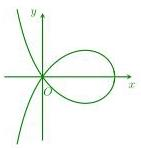
\includegraphics[max width=0.2\textwidth]{images/bo_d7fr3gc91nqc7381iccg_168_1325_737_141_148_0.jpg}
\end{center}
\hspace*{3em} 

11. 设计一条美丽的丝带,其造型 \(\smallsetminus   \text{ ○ }\) 可以看作图中的曲线 \(C\) 的一部分,已知 \(C\) 过坐标原点 \(O\) ,且 \(C\) 上的点满足横坐标大于 -2,到点 \(F\left( {2,0}\right)\) 的距离与到定直线 \(x = a\left( {a < 0}\right)\) 的距离之积为 4 , 则 ( )

A. \(a =  - 2\)

B. 点 \(\left( {2\sqrt{2},0}\right)\) 在 \(C\) 上

C. \(C\) 在第一象限的点的纵坐标的最大值为 1

D. 当点 \(\left( {{x}_{0},{y}_{0}}\right)\) 在 \(C\) 上时, \({y}_{0} \leq  \frac{4}{{x}_{0} + 2}\)

17. 如图,四棱锥 \(P - {ABCD}\) 中, \({PA} \bot\) 底面 \({ABCD},{PA} = {AC} = 2,{BC} = 1,{AB} = \sqrt{3}\) . ( 1 ) 若 \({AD} \bot  {PB}\) ,证明: \({AD}//\) 平面 \({PBC}\) ;

( 2 ) 若 \({AD} \bot  {DC}\) ,且二面角 \(A - {CP} - D\) 的正弦值为 \(\frac{\sqrt{42}}{7}\) ,求 \({AD}\) .

\begin{center}
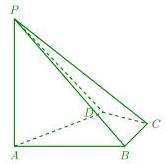
\includegraphics[max width=0.2\textwidth]{images/bo_d7fr3gc91nqc7381iccg_168_1314_1236_166_164_0.jpg}
\end{center}
\hspace*{3em} 

18. 已知函数 \(f\left( x\right)  = \ln \frac{x}{2 - x} + {ax} + b{\left( x - 1\right) }^{3}\)

( 1 ) 若 \(b = 0\) ,且 \({f}^{\prime }\left( x\right)  \geq  0\) ,求 \(a\) 的最小值;

( 2 ) 证明: 曲线 \(y = f\left( x\right)\) 是中心对称图形;

( 3 ) 若 \(f\left( x\right)  >  - 2\) ,当且仅当 \(1 < x < 2\) ,求 \(b\) 的取值范围.

19. 设 \(m\) 为正整数,数列 \({a}_{1},{a}_{2},\cdots ,{a}_{{4m} + 2}\) 是公差不为 0 的等差数列,若从中删去两项 \({a}_{i}\) 和 \({a}_{j}\left( {i < j}\right)\) 后剩余的 \({4m}\) 项可被平均分为 \(m\) 组,且每组的 4 个数都能构成等差数列,则称数列 \({a}_{1},{a}_{2},\cdots ,{a}_{{4m} + 2}\) 是 \(\left( {i,j}\right)\) - 可分数列.

( 1 ) 写出所有的 \(\left( {i,j}\right) ,1 \leq  i < j \leq  6\) ,使数列 \({a}_{1},{a}_{2},\cdots ,{a}_{6}\left( {i,j}\right)\) - 可分数列;

( 2 ) 当 \(m \geq  3\) 时,证明: 数列 \({a}_{1},{a}_{2},\cdots ,{a}_{{4m} + 2}\) 是 \(\left( {2,{13}}\right)\) - 可分数列;

( 3 ) 从 \(1,2,\cdots ,{4m} + 2\) 中一次任取两个数 \(i\) 和 \(j\left( {i < j}\right)\) ,记数列 \({a}_{1},{a}_{2},\cdots ,{a}_{{4m} + 2}\) 是 \(\left( {i,j}\right)\) - 可分数列的概率为 \({P}_{m}\) ,证明 \({P}_{m} > \frac{1}{8}\) .

\section*{试题 + 答案版本和纯答案版本}

按秘密事项管理 \ding{72} 启用前 【解答】

2022 年普通高等学生招生全国统一考试 (模拟卷) 4.

( )

数 学 A. B. C. D.

【考试声明】

【分析】

【简要答案】

1. 认真考试，不要作弊，可以百度答案，但是百度不了人生; 【解答】

5.

2. 把答案写到答题卡上;

3. 参考公式:我就不写了；

( )

一、选择题:本大题共 12 小题，每小题 5 分，共 60 分。在每小题给出的四个选项中，只有一项是符合题目要求的。 A. B. C. D.

【分析】

1. 【简要答案】

( ) 【解答】

A. B. C. 6.

【分析】 ( )

【简要答案】 A. B. C. D.

【解答】 【分析】

2. 【简要答案】

( ) 【解答】

A. B. C. 7.

【分析】 ( )

【简要答案】 A. B. C. D.

【解答】 【分析】

3. 【简要答案】

【解答】

A. B. C. D. 8.

【分析】

【简要答案】

按秘密事项管理 \ding{72} 启用前 7.【分析】

2022 年普通高等学生招生全国统一考试(模拟卷) 【简要答案】

【解答】

数 学 8.【分析】

【考试声明】

【简要答案】

【解答】

1. 认真考试, 不要作弊, 可以百度答案, 但是百度不了人生;

9.【分析】

2. 把答案写到答题卡上;

【简要答案】

3. 参考公式:我就不写了；

【解答】

一、选择题:本大题共 12 小题，每小题 5 分，共 60 分。在每小题给出的四个选项中，只有一项是符合题目要求的。 10.【分析】

【简要答案】

1.【分析】 【解答】

【简要答案】 11.【分析】

【解答】 【简要答案】

2.【分析】 【解答】

【简要答案】 12.【分析】

【解答】 【简要答案】

3.【分析】 【解答】

【简要答案】 二、填空题:本大题共 4 小题，每小题 5 分，共 20 分。把答案填写在题中的横线上。

【解答】 13.【分析】

4.【分析】 【简要答案】

【简要答案】 【解答】

14.【分析】

5.【分析】 【简要答案】

【简要答案】 【解答】

【解答】 15.【分析】

6.【分析】 【简要答案】

【简要答案】 【解答】

【解答】 16.【分析】

第 1 页 共 2 页

讲义

\section*{导数 函数单调性的讨论}

\section*{觅宁参考出品}

\section*{【主要内容】}

口典例精炼 3. 含参二次函数单调性的讨论

1. 含参一次函数单调性的讨论 4. 类含参二次函数单调性的讨论

2. 类含参一次函数单调性的讨论 5. 超越函数的零点问题

\section*{【核心逻辑】}

讨论参数的不同，得到导函数的单调性和导函数零点判断导函数在相应区间的正负，进而判断原函数的单调性.

\section*{【问题方法】}

一、求不含参函数的单调区间

1. 求函数定义域 易漏

2. 求出原函数的导函数,解出 \({f}^{\prime }\left( x\right)  = 0\) 的根 \({x}_{1},{x}_{2},\cdots\) ;

3. 用 \({x}_{1},{x}_{2},\cdots\) 将定义域划分为若干单调区间,分别计算每个区间上导函数的正负值;

4. 画出原函数的草图检验, 然后总结作答.

注意 若相邻两个单调区间的单调性一致, 则可视为一个单调区间.

二、含参一次函数单调性的讨论

1. 讨论最高次项是否为 0 ，正负情况 易漏

2. 求解导函数的根;

3. 定义域划分为若干单调区间, 分别讨论每个区间上导函数的正负值.

三、含参二次函数单调性的讨论

核心逻辑 就是三讨论: 讨论开口方向、讨论两根大小、讨论根的数量.

讨论开口方向观察二次项系数是否含参，如果含参，注意讨论开口方向(包括是否为 0 \()\) . 易漏

讨论两根大小观察能否分解因式, 能分解因式的, 注意比较两根大小, 以及两根

是否相等;

讨论根的数量如果不能分解因式, 计算判别式, 根据情况讨论;

方法步骤

(1)求函数定义域，求出原函数的导函数

(2)讨论最高次项是否为 0，正负情况；

(a) \(\left\{  \begin{array}{l} \text{ 可以分解因式 } \Rightarrow  \text{ 解得 }{x}_{1},{x}_{2}\text{ (注意讨论 }{x}_{1} = {x}_{2}\text{ ) } \\  \text{ 不能分解 } \Rightarrow  \left\{  \begin{array}{l} \Delta  \leq  0 \\  \Delta  > 0 \end{array}\right.  \end{array}\right.\)

(3)讨论 \({x}_{1}\) 和 \({x}_{2}\) 的大小，能分解因式的，注意讨论 \({x}_{1} = {x}_{2}\) .

(4) \({x}_{1}\) ， \({x}_{2}\) 将定义域划分为若干单调区间，分别讨论每个区间上导函数的正负值. 四、超越函数的零点问题

超越函数的零点, 关键在于零点的求解, 而一般超越函数的零点是不可解, 那么我们的方法有三:

1. 从题意中获取.

2. 试根. 一般是让对数式、指数式等于 0 或 1 等特殊值.

3. 零点本身不可解. 一般求出零点满足的关系式与取值范围，用 \({x}_{0}\) 表示这个零点, 这就是通常所说的隐零点.

\section*{【知识清单】}

在某个区间 \(\left( {a,b}\right)\) 内,

如果 \({f}^{\prime }\left( x\right)  > 0\) ,那么函数 \(y = f\left( x\right)\) 在这个区间内单调递增;

如果 \({f}^{\prime }\left( x\right)  < 0\) ,那么函数 \(y = f\left( x\right)\) 在这个区间内单调递减.

***典例精练***

\section*{一、对回归方程的理解}

1. (2012 湖南理 4(4/8) \ding{72}  \ding{73}  \ding{73}  \ding{73}  \ding{73}  \ding{73} )

设某大学的女生体重 \(y\) (单位: \(\mathrm{{kg}}\) ) 与身高 \(x\) (单位: \(\mathrm{{cm}}\) ) 具有线性相关关系,根据一组样本数据 \(\left( {{x}_{i},{y}_{i}}\right) \left( {i = 1,2,\cdots ,n}\right)\) ,用最小二乘法建立的回归方程为 \(y = \; {0.85x} - {85.71}\) ,则下列结论中不正确的是

A. \(y\) 与 \(x\) 具有正的线性相关关系

B. 回归直线过样本点的中心 \(\left( {\bar{x},\bar{y}}\right)\)

C. 若该大学某女生身高增加 \(1\mathrm{\;{cm}}\) ，则其体重约增加 \({0.85}\mathrm{\;{kg}}\)

D. 若该大学某女生身高为 170 cm，则可断定其体重必为 58.79 kg

2. (2012 全国 I 文 \(3\left( {3/{12}}\right)  \star   \star   \star   \star   \star   \star\) 交

在一组样本数据 \(\left( {{x}_{i},{y}_{1}}\right) ,\left( {{x}_{2},{y}_{2}}\right) ,\cdots ,\left( {{x}_{n},{y}_{n}}\right) \left( {n \geq  2,{x}_{1},{x}_{2},\cdots ,{x}_{n}}\right.\) 不全相等) 的散点图中,若所有样本点 \(\left( {{x}_{i},{y}_{i}}\right) \left( {i = 1,2,\cdots ,n}\right)\) 都在直线 \(y = \frac{1}{2}x + 1\) 上,则这组样本数据的样本相关关系为 ( )

A. -1 B. 0 C. \(\frac{1}{2}\) D. 1

3. (2014 湖北理 4 文 \(6\left( {4/{10}}\right)\)  \ding{72}  \ding{73}  \ding{73}  \ding{73}  \ding{73} )

根据如下样本数据

\begin{center}
\adjustbox{max width=\textwidth}{
\begin{tabular}{|c|c|c|c|c|c|c|c|}
\hline
\phantom{X} & \(x\) & 3 & 4 & 5 & 6 & 7 & 8 \\
\cline{1-8}
\phantom{X} & \(y\) & 4.0 & 2.5 & -0.5 & 0.5 & -2.0 & -3.0 \\
\cline{1-8}
\hline
\end{tabular}
}
\end{center}

得到的回归方程为 \(\widehat{y} = {bx} + a\) ,则 ( )

A. \(a > 0,b < 0\) B. \(a > 0,b > 0\)

C. \(a < 0,b < 0\) D. \(a < 0,b > 0\)

二、回归直线过样本中心

4. (2014 重庆理 \(3\left( {3/{10}}\right)  \star   \star\) 奇奇奇

已知变量 \(x\) 与 \(y\) 正相关,且由观测数据算得样本的平均数 \(\widetilde{x} = {2.5},\widetilde{y} = {3.5}\) ,则由观测的数据得线性回归方程可能为 ( )

A. \(\widehat{y} = {0.4x} + {2.3}\) B. \(\widehat{y} = {2x} - {2.4}\)

C. \(\widehat{y} =  - {2x} + {9.5}\) D. \(\widehat{y} =  - {0.3x} + {4.4}\)

5. (2011 山东理 \(7\left( {7/{12}}\right) 4\bigstar 4\text{  \ding{73}  }4\) )

某产品的广告费用 \(x\) 与销售额 \(y\) 的统计数据如下表

\begin{center}
\adjustbox{max width=\textwidth}{
\begin{tabular}{|c|c|c|c|c|}
\hline
广告费用 \(x\) (万元) & 4 & 2 & 3 & 5 \\
\cline{1-5}
销售额 \(y\) (万元) & 49 & 26 & 39 & 54 \\
\cline{1-5}
\hline
\end{tabular}
}
\end{center}

根据上表可得回归方程 \(\widehat{y} = \widehat{b}x + \widehat{a}\) 中的 \(\widehat{b}\) 为 9.4,据此模型预报广告费用为 6 万元时销售额为 ( )

A. 63.6 万元 B. 65.5 万元 C. 67.7 万元 D. 72.0 万元

6. (2015 福建理 4(4/10) \ding{72}  \ding{72}  \ding{73}  \ding{73}  \ding{73} )

为了解某社区居民的家庭年收入所年支出的关系，随机调查了该社区 5 户家庭， 得到如下统计数据表

\begin{center}
\adjustbox{max width=\textwidth}{
\begin{tabular}{|c|c|c|c|c|c|}
\hline
收入 x(万元) & 8.2 & 8.6 & 10.0 & 11.3 & 11.9 \\
\cline{1-6}
支出 y(万元) & 6.2 & 7.5 & 8.0 & 8.5 & 9.8 \\
\cline{1-6}
\hline
\end{tabular}
}
\end{center}

根据上表可得回归直线方程 \(\widehat{y} = \widehat{b}x + \widehat{a}\) ,其中 \(\widehat{b} = {0.76},\widehat{a} = \bar{y} - \widehat{b}\bar{x}\) ,据此估计,该社区一户收入为 15 万元家庭年支出为 ( )

A. 11.4 万元 B. 11.8 万元 C. 12.0 万元 D. 12.2 万元

7. (2017 山东理 \(5\left( {5/{10}}\right)  \star   \star   \star   \star   \star\) )

为了研究某班学生的脚长 \(x\) (单位: 厘米) 和身高 \(y\) (单位: 厘米) 的关系,从该班随机抽取 10 名学生,根据测量数据的散点图可以看出 \(y\) 与 \(x\) 之间有线性相关关系. 设其回归直线方程为 \(\widehat{y} = \widehat{b}x + \widehat{a}\) . 已知 \(\mathop{\sum }\limits_{{i = 1}}^{{10}}{x}_{i} = {225},\mathop{\sum }\limits_{{i = 1}}^{{10}}{y}_{i} = {1600},\widehat{b} = 4\) . 该班某同学的脚长为 24 ，据此估计其身高为 ( )

A. 160 B. 163 C. 166 D. 170

8.( \ding{72}  \ding{72}  \ding{72}  \ding{73}  \ding{73} )

两个相关变量满足如下关系:

\begin{center}
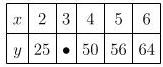
\includegraphics[max width=0.2\textwidth]{images/bo_d7fr3gc91nqc7381iccg_170_1110_1993_163_67_0.jpg}
\end{center}
\hspace*{3em} 

\section*{校本教材}

专题 1 标题

知识框架

(1)

二、 (2)

1. (a)

2. (b)

一、大类知识点

1、小题型

例1  \ding{72}  \ding{72}  \ding{72}  \ding{72}  \ding{72} 

微信公众号《觅宁参考》制作 微信公众号《觅宁参考》制作 微信公众号《觅宁参考》制作 微信公众号《觅宁参考》制作 微信公众号《觅宁参考》制作 微信公众号 《觅宁参考》制作 微信公众号《觅宁参考》制作 ( )

A. B. C. D.

【简要答案】

练 1.1 微信公众号《觅宁参考》制作 微信公众号《觅宁参考》制作 微信公众号《觅宁参考》制作 微信公众号《觅宁参考》制作 微信公众号《觅宁参考》制作 微信公众号《觅宁参考》制作 微信公众号《觅宁参考》制作 ( )

A. D.

【简要答案】

知识总结

微信公众号《觅宁参考》制作 微信公众号《觅宁参考》制作 微信公众号《觅宁参考》制作 微信公众号《觅宁参考》制作 微信公众号

号《觅宁参考》制作 微信公众号《觅 《觅宁参考》制作 微信公众号《觅宁参考》制作

抛物线知识清单

\section*{【知识清单】}

一、概念性质

定义 平面内与一个定点 \(F\) 和一条定直线 \(l\left( l\right.\) 不经过点 \(F\) ) 距离相等的点的轨迹叫做抛物线. 点 \(F\) 叫做抛物线的焦点,直线 \(l\) 叫做抛物线的 准线.

\section*{几何性质}

\begin{center}
\adjustbox{max width=\textwidth}{
\begin{tabular}{|c|c|c|c|c|}
\hline
标准方程 \(\left( {p > 0}\right)\) & \({y}^{2} = {2px}\) & \({y}^{2} =  - {2px}\) & \({x}^{2} = {2py}\) & \({x}^{2} =  - {2py}\) \\
\cline{1-5}
图象 & 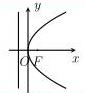
\includegraphics[max width=0.2\textwidth]{images/bo_d7fr3gc91nqc7381iccg_171_374_1510_85_93_0.jpg} & 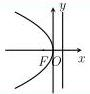
\includegraphics[max width=0.2\textwidth]{images/bo_d7fr3gc91nqc7381iccg_171_483_1510_90_94_0.jpg} & 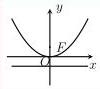
\includegraphics[max width=0.2\textwidth]{images/bo_d7fr3gc91nqc7381iccg_171_587_1512_100_89_0.jpg} & 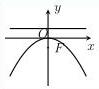
\includegraphics[max width=0.2\textwidth]{images/bo_d7fr3gc91nqc7381iccg_171_699_1512_99_89_0.jpg} \\
\cline{1-5}
开口方向 & 向右 & 向左 & 向上 & 向下 \\
\cline{1-5}
焦点坐标 & \(P\left( {\frac{p}{2},0}\right)\) & \(P\left( {-\frac{p}{2},0}\right)\) & \(P\left( {0,\frac{p}{2}}\right)\) & \(P\left( {0, - \frac{p}{2}}\right)\) \\
\cline{1-5}
准线方程 & \(x =  - \frac{p}{2}\) & \(x = \frac{p}{2}\) & \(y =  - \frac{p}{2}\) & \(y = \frac{p}{2}\) \\
\cline{1-5}
对称轴 & \multicolumn{2}{|c|}{\(y = 0\)} & \multicolumn{2}{|c|}{\(x = 0\)} \\
\cline{1-5}
顶点坐标 & \multicolumn{4}{|c|}{\(\left( {0,0}\right)\)} \\
\cline{1-5}
离心率 & \multicolumn{4}{|c|}{\(e = 1\) (到定点与到定直线的距离之比称之为离心率)} \\
\cline{1-5}
\hline
\end{tabular}
}
\end{center}

总结记忆

1. 抛物线方程一定首先转化为标准方程;

2. 焦点与一次项保持一致;

3. 焦点到原点的距离为一次项系数的 \(\frac{1}{4}\)

课后练习

1.

( )

A. B. C. D.

【简要答案】

2.

( )

A. B. C. D.

【简要答案】

二、二级结论

1. 焦点弦 \(\left( {p > 0}\right)\)

\begin{center}
\adjustbox{max width=\textwidth}{
\begin{tabular}{|c|c|c|c|c|}
\hline
标准方程 & \({y}^{2} = {2px}\) & \({y}^{2} =  - {2px}\) & \({x}^{2} = {2py}\) & \({x}^{2} =  - {2py}\) \\
\cline{1-5}
焦点弦韦达定理 & \multicolumn{2}{|c|}{\({y}_{1}{y}_{2} =  - {p}^{2},{x}_{1}{x}_{2} = \frac{{p}^{2}}{4}\)} & \multicolumn{2}{|c|}{\({x}_{1}{x}_{2} =  - {p}^{2},{y}_{1}{y}_{2} = \frac{{p}^{2}}{4}\)} \\
\cline{1-5}
焦半径与坐标 & \({x}_{0} + \frac{p}{2}\) & \(- {x}_{0} + \frac{p}{2}\) & \({y}_{0} + p\) & \(- {y}_{0} + \frac{p}{2}\) \\
\cline{1-5}
焦半径与倾斜角 & \multicolumn{2}{|c|}{\(\left| {AF}\right|  = \frac{p}{1 - \cos \theta },\left| {BF}\right|  = \frac{p}{1 + \cos \theta }\) 点 \(A\) 在 \(x\) 轴上方} & \multicolumn{2}{|c|}{\(\left| {AF}\right|  = \frac{p}{1 - \sin \theta },\left| {AF}\right|  = \frac{p}{1 + \sin \theta }\) 注意焦半径小的分母较大} \\
\cline{1-5}
推论 & \multicolumn{2}{|c|}{以 \({AF}\) (或 \({BF}\) ) 为直径的圆与 \(y\) 轴相切} & \multicolumn{2}{|c|}{以 \({AF}\) (或 \({BF}\) ) 为直径的圆与 \(x\) 轴相切} \\
\cline{1-5}
焦半径与定值 & \multicolumn{4}{|c|}{\(\frac{1}{\left| AF\right| } + \frac{1}{\left| BF\right| }\) 为定值为 \(\frac{2}{p}\)} \\
\cline{1-5}
焦点弦长与坐标 & \({x}_{1} + {x}_{2} + p\) & \(- {x}_{1} - {x}_{2} + p\) & \({y}_{1} + {y}_{2} + p\) & \(- {y}_{1} - {y}_{2} + p\) \\
\cline{1-5}
焦点弦长与倾斜角 & \multicolumn{2}{|c|}{\(\left| {AB}\right|  = \frac{2p}{{\sin }^{2}\theta }\)} & \multicolumn{2}{|c|}{\(\left| {AB}\right|  = \frac{2p}{{\cos }^{2}\theta }\)} \\
\cline{1-5}
通径 & \multicolumn{4}{|c|}{最短的焦点弦为通径长为 \({2p}\)} \\
\cline{1-5}
\({S}_{\bigtriangleup {OAB}}\) & \multicolumn{2}{|c|}{\(\frac{{p}^{2}}{2\sin \theta }\)} & \multicolumn{2}{|c|}{\(\frac{{p}^{2}}{2\cos \theta }\)} \\
\cline{1-5}
推论 & \multicolumn{4}{|c|}{以 \({AB}\) 为直径的圆与准线相切,记切点为 \(P\) ,则 \(\angle {APB} = {90}^{ \circ  }\)} \\
\cline{1-5}
\hline
\end{tabular}
}
\end{center}

2. 中点弦

\({y}^{2} = {2px}\) 与 \(y = {kx} + b\) 交于 \(A,B\) 两点,记 \({AB}\) 中点为 \(\left( {{x}_{0},{y}_{0}}\right)\) ,则有 \(\underline{k{y}_{0} = p}\) ; \({x}^{2} = {2py}\) 与 \(y = {kx} + b\) 交于 \(A,B\) 两点,记 \({AB}\) 中点为 \(\left( {{x}_{0},{y}_{0}}\right)\) ,则有 \(\frac{1}{k}{x}_{0} = p\) ;

\section*{幻灯片}

二、探究新知，动手操作

(一)探究新知，回顾背景

\begin{center}
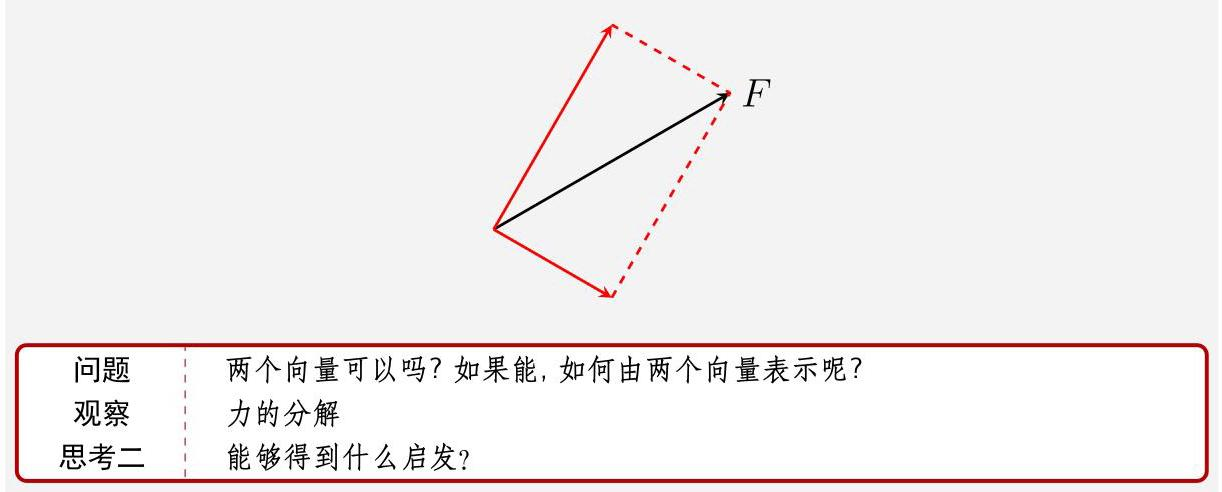
\includegraphics[max width=1.0\textwidth]{images/bo_d7fr3gc91nqc7381iccg_172_215_416_1222_492_0.jpg}
\end{center}
\hspace*{3em} 

觅宁参考 §6.3.1 平面向量基本定理 3 / 11

二、探究新知，动手操作

(一) 探究新知, 回顾背景

\begin{center}
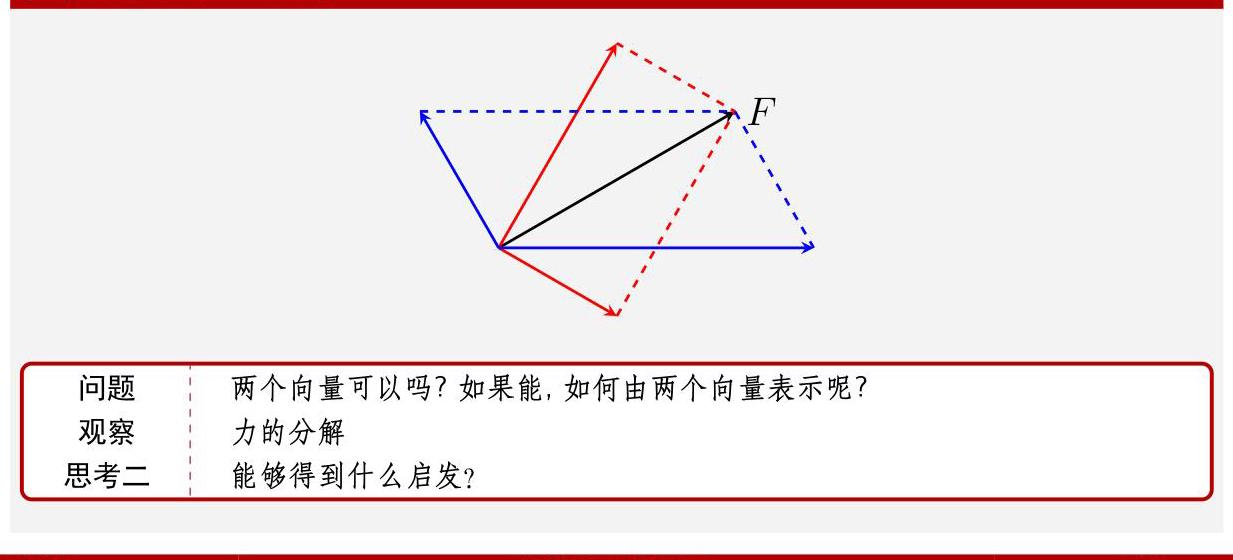
\includegraphics[max width=1.0\textwidth]{images/bo_d7fr3gc91nqc7381iccg_172_210_1109_1233_560_0.jpg}
\end{center}
\hspace*{3em} 

1. IATEX 本身都可以画出高清矢量图, 同时图中的元素也可以轻松实现逐步显示;

2. 类似地, 图中的文字、公式也可以轻松实现逐步显示, 并且自动对齐;

3. 公式中的数字等实现逐步显示是其他很多软件无法实现的.

\section*{二、探究新知, 动手操作}

(二) 探究新知, 动手操作

\begin{center}
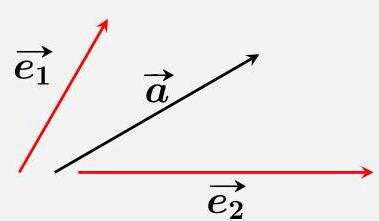
\includegraphics[max width=0.3\textwidth]{images/bo_d7fr3gc91nqc7381iccg_173_402_367_379_221_0.jpg}
\end{center}
\hspace*{3em} 

\begin{center}
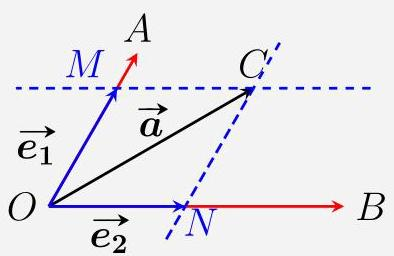
\includegraphics[max width=0.3\textwidth]{images/bo_d7fr3gc91nqc7381iccg_173_845_333_394_256_0.jpg}
\end{center}
\hspace*{3em} 

\[
\overrightarrow{OC} = \overrightarrow{OM} + \overrightarrow{ON}
\]

\[
\overrightarrow{OM} = {\lambda }_{1}\overrightarrow{OA},\overrightarrow{ON} = {\lambda }_{2}\overrightarrow{OB},
\]

\[
\overrightarrow{OC} = {\lambda }_{1}\overrightarrow{OA} + {\lambda }_{2}\overrightarrow{OB}
\]

\begin{itemize}\relax
\item\relax GeoGebra 动态演示
\end{itemize}

觅宁参考 §6.3.1 平面向量基本定理

裂项相消的一般步骤

例 1

已知数列 \({b}_{n} = \frac{2}{\left( {{2n} - 1}\right) \left( {{2n} + 1}\right) }\) ,求其前 \(n\) 项和 \({S}_{n}\) .

解答

因为 \({b}_{n} = \frac{2}{\left( {{2n} - 1}\right) \left( {{2n} + 1}\right) } = \frac{1}{{2n} - 1} - \frac{1}{{2n} + 1}\) , 对通项裂项

所以 \({S}_{n} = {b}_{1} + {b}_{2} + {b}_{3}\cdots  + {b}_{n - 1} + {b}_{n}\) 求谁表示谁

\(= \left( {\frac{1}{1} - \frac{1}{3}}\right)  + \left( {\frac{1}{3} - \frac{1}{5}}\right)  + \left( {\frac{1}{5} - \frac{1}{7}}\right)  + \cdots  + \left( {\frac{1}{{2n} - 3} - \frac{1}{{2n} - 1}}\right)  + \left( {\frac{1}{{2n} - 1} - \frac{1}{{2n} + 1}}\right)\) 代进去

\(= 1 - \frac{1}{{2n} + 1}\) 消去

\(= \frac{2n}{{2n} + 1}\) 化简

4. 方便对题干、解答做批注, 可以非常方面的提示、引导学生;

5. 试卷、讲义和幻灯片中的内容可以互相复制粘贴, 无需过多调整, 互相兼容性好.

6. 样式简约美观, 格式自动排版, 教师只需要专注内容, 无需花大量时间到格式调整上, 效率高.

\section*{2.5 数学作图方便、精准、美观与文档浑然一体}

\begin{itemize}\relax
\item\relax 函数图象
\end{itemize}

\begin{center}
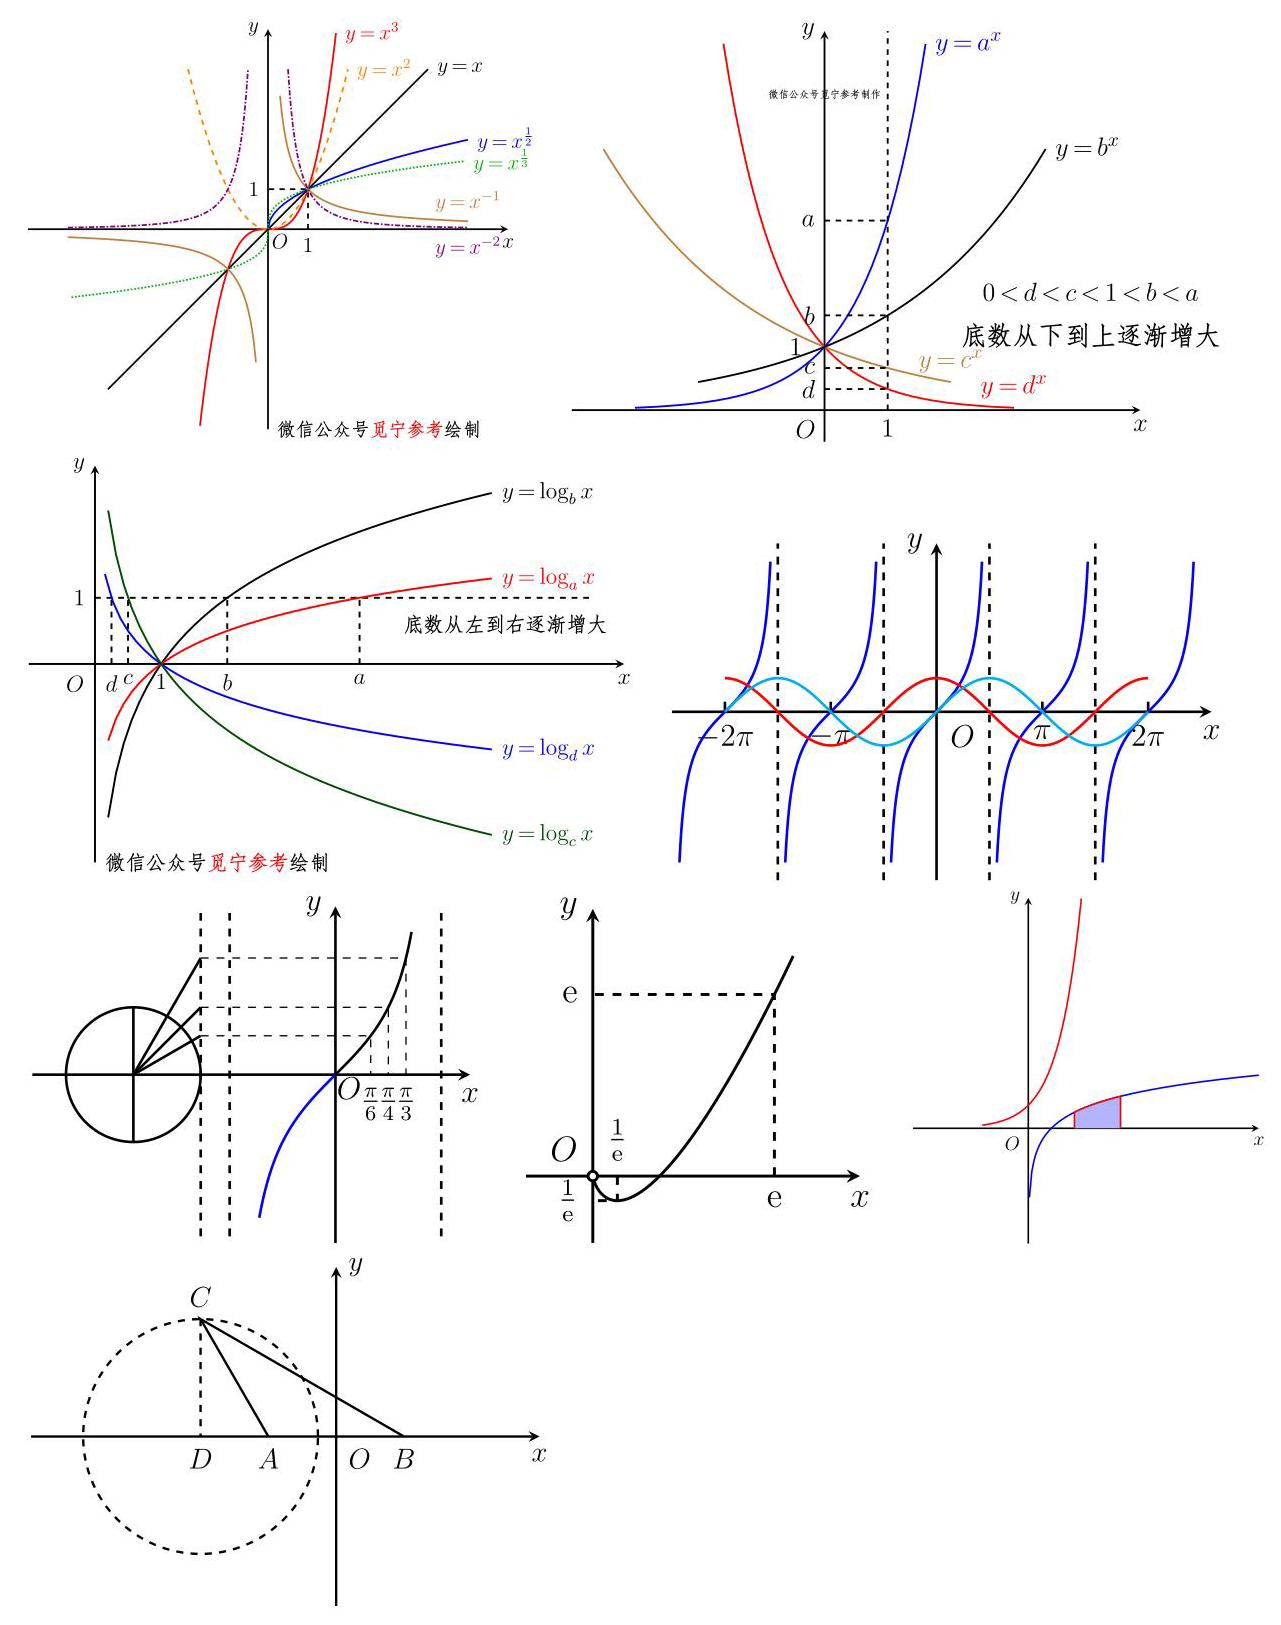
\includegraphics[max width=1.0\textwidth]{images/bo_d7fr3gc91nqc7381iccg_174_238_382_1281_1625_0.jpg}
\end{center}
\hspace*{3em} 

+ 立体几何

\begin{center}
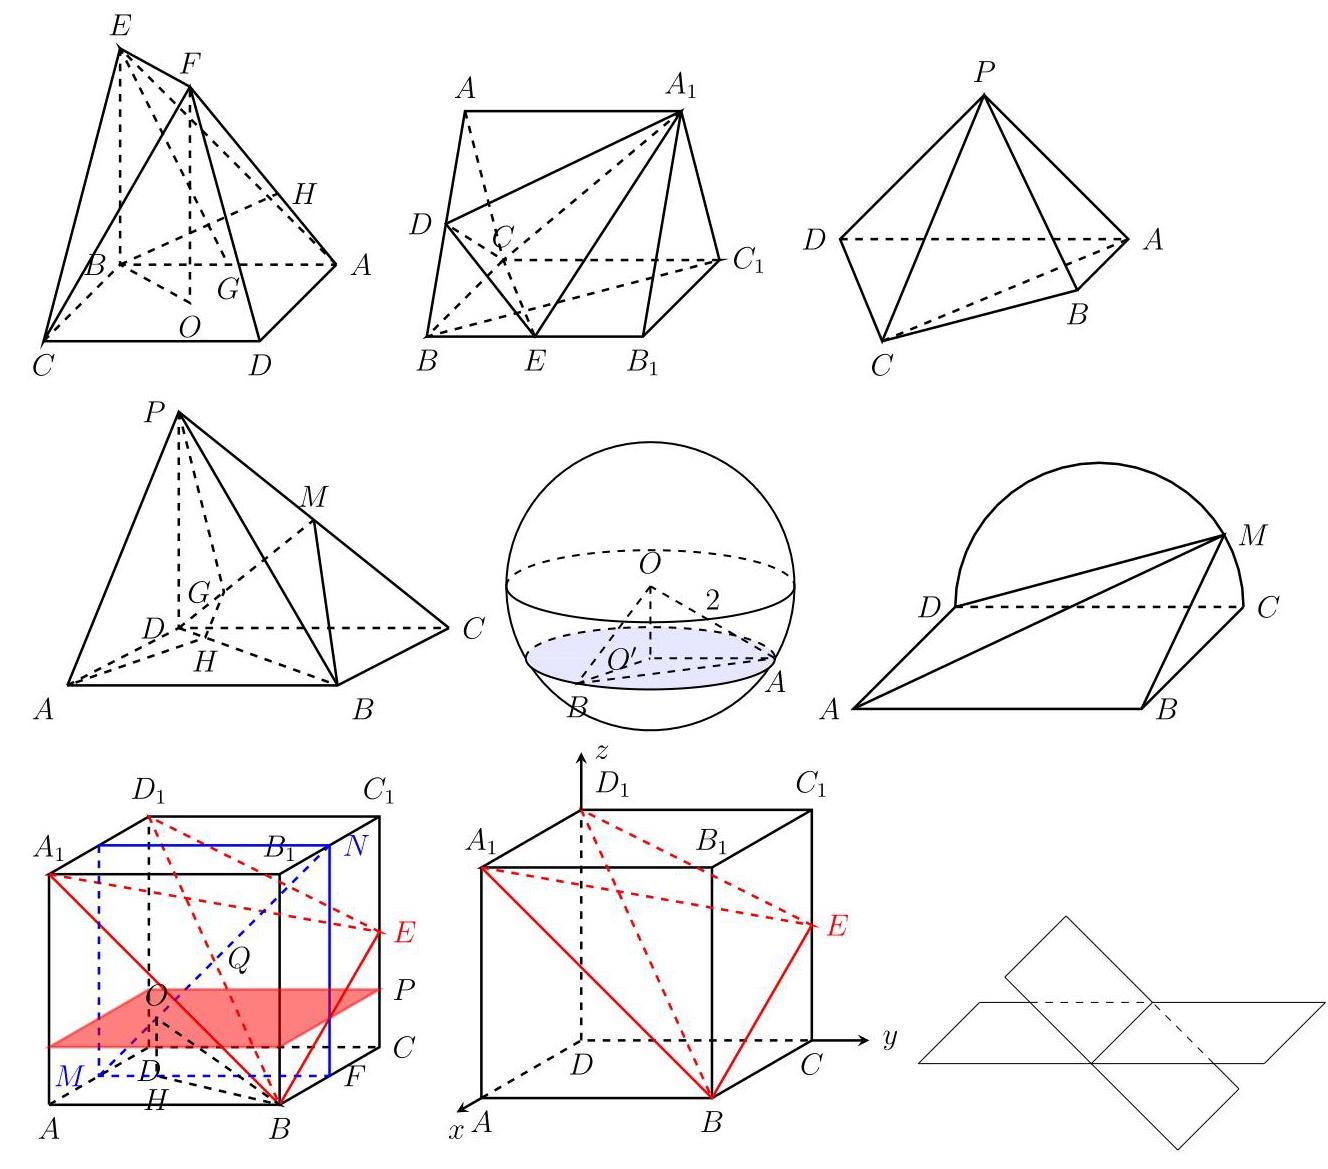
\includegraphics[max width=1.0\textwidth]{images/bo_d7fr3gc91nqc7381iccg_175_237_357_1328_1169_0.jpg}
\end{center}
\hspace*{3em} 

统计图

\begin{center}
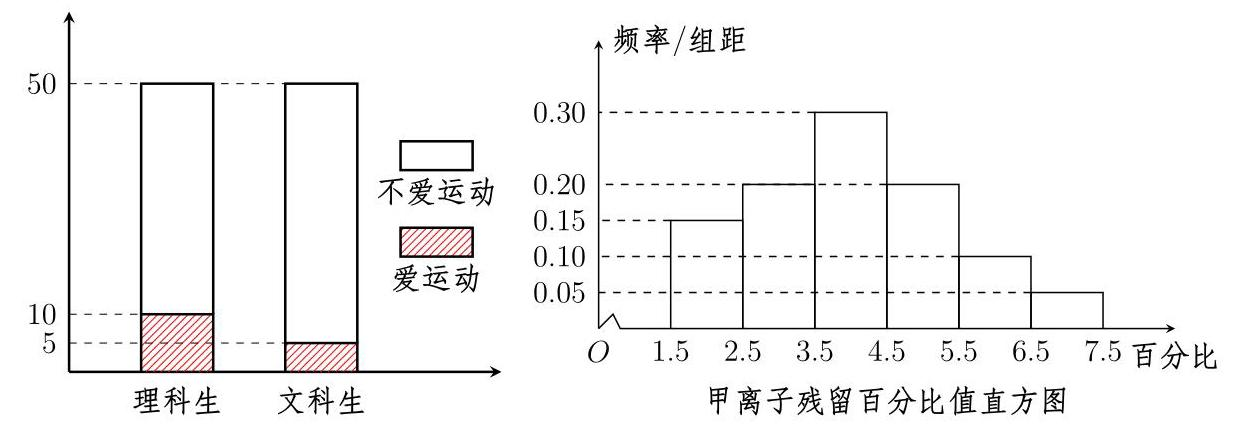
\includegraphics[max width=1.0\textwidth]{images/bo_d7fr3gc91nqc7381iccg_175_242_1643_1243_433_0.jpg}
\end{center}
\hspace*{3em} 

关注微信公众号《觅宁参考》免费下载软件、教程, 添加微信与作者交流第 13 页 共 20 页

\begin{center}
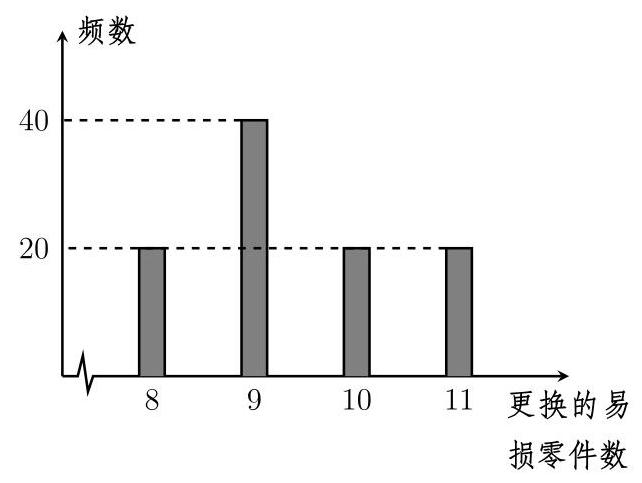
\includegraphics[max width=0.5\textwidth]{images/bo_d7fr3gc91nqc7381iccg_176_222_295_642_483_0.jpg}
\end{center}
\hspace*{3em} 

\begin{center}
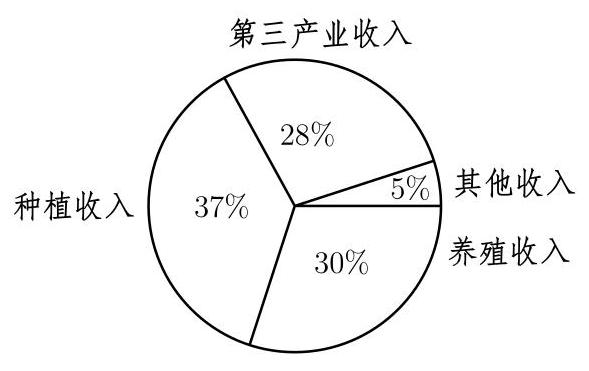
\includegraphics[max width=0.5\textwidth]{images/bo_d7fr3gc91nqc7381iccg_176_879_333_589_371_0.jpg}
\end{center}
\hspace*{3em} 

建设后经济收入构成比例

\begin{itemize}\relax
\item\relax 圆锥曲线的图
\end{itemize}

\(y\)

-0

\begin{center}
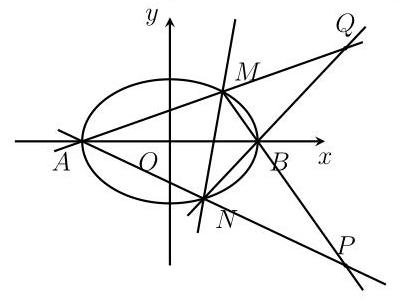
\includegraphics[max width=0.3\textwidth]{images/bo_d7fr3gc91nqc7381iccg_176_225_1222_398_301_0.jpg}
\end{center}
\hspace*{3em} 

\section*{4 其他平面图形}

\begin{center}
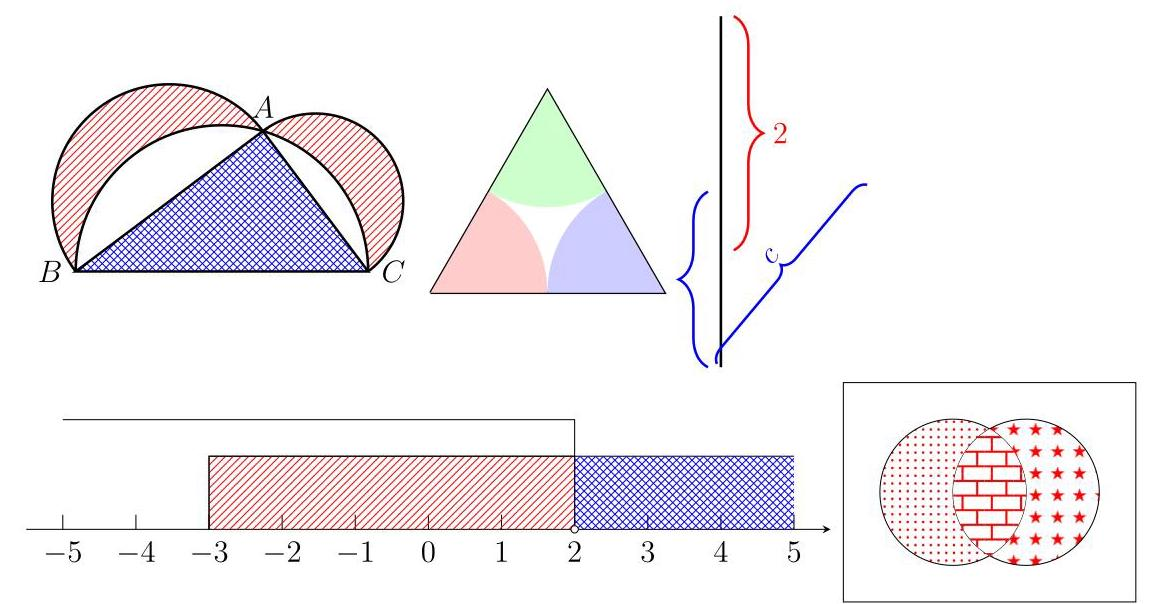
\includegraphics[max width=0.9\textwidth]{images/bo_d7fr3gc91nqc7381iccg_177_203_347_1154_604_0.jpg}
\end{center}
\hspace*{3em} 

+ 其它图形

\begin{center}
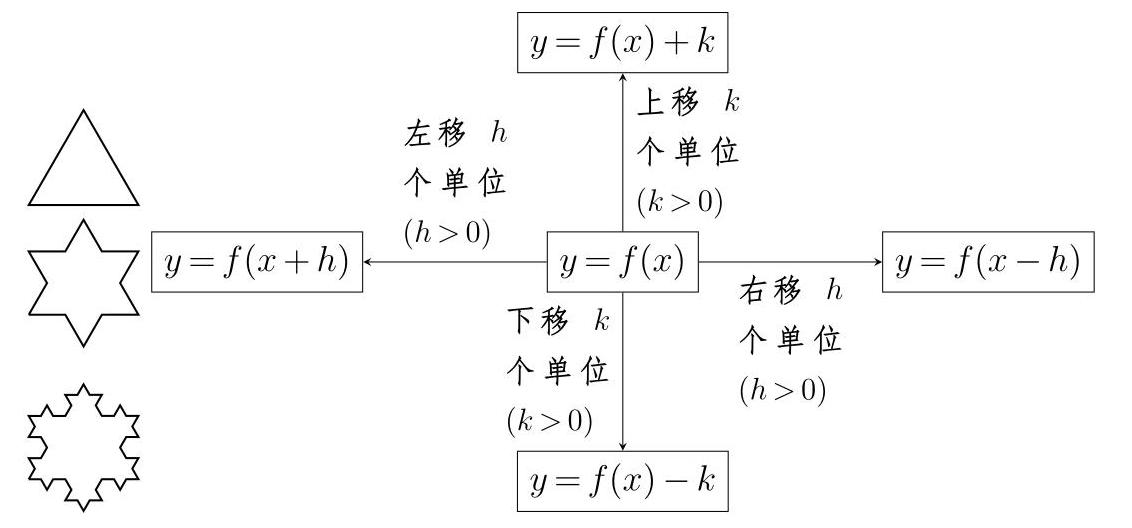
\includegraphics[max width=0.9\textwidth]{images/bo_d7fr3gc91nqc7381iccg_177_201_1085_1132_528_0.jpg}
\end{center}
\hspace*{3em} 

+ 三视图

\begin{center}
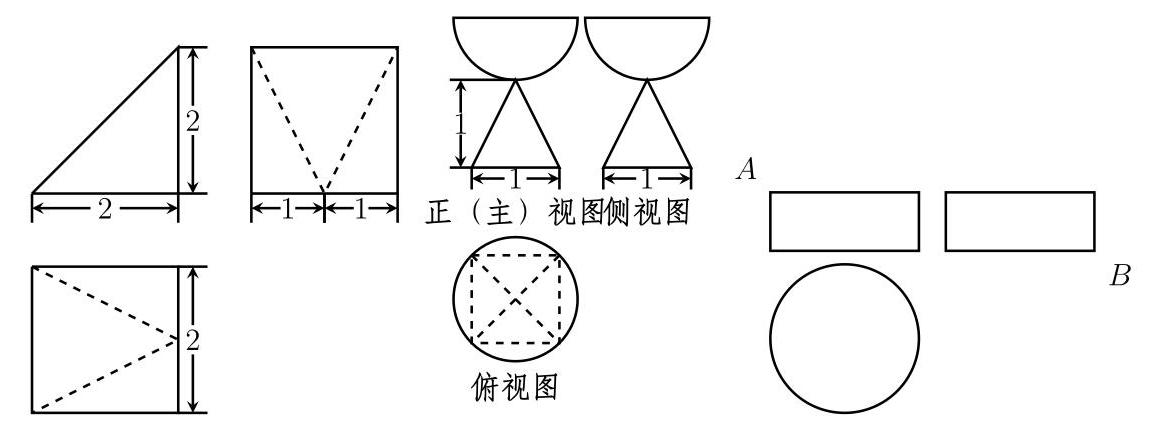
\includegraphics[max width=0.9\textwidth]{images/bo_d7fr3gc91nqc7381iccg_177_198_1728_1150_428_0.jpg}
\end{center}
\hspace*{3em} 

\section*{与文档浑然一体}

\section*{三、指对幂的函数图象}

\section*{例 6 \(\left( {\bigstar \bigstar \text{  \ding{73}  }\text{  \ding{73}  }\text{  \ding{73}  }}\right)\)}

已知 \({y}_{1} = {\left( \frac{1}{3}\right) }^{x},{y}_{2} = {3}^{x},{y}_{3} = {10}^{-x},{y}_{4} = {10}^{x}\) ,则在同一直角坐标系内,他们的图象为 ( )

\begin{center}
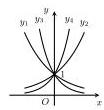
\includegraphics[max width=0.2\textwidth]{images/bo_d7fr3gc91nqc7381iccg_178_321_371_104_110_0.jpg}
\end{center}
\hspace*{3em} 

A

\begin{center}
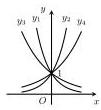
\includegraphics[max width=0.2\textwidth]{images/bo_d7fr3gc91nqc7381iccg_178_453_372_101_110_0.jpg}
\end{center}
\hspace*{3em} 

B

\begin{center}
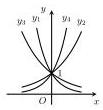
\includegraphics[max width=0.2\textwidth]{images/bo_d7fr3gc91nqc7381iccg_178_582_372_103_110_0.jpg}
\end{center}
\hspace*{3em} 

C

\begin{center}
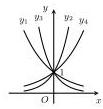
\includegraphics[max width=0.2\textwidth]{images/bo_d7fr3gc91nqc7381iccg_178_709_373_103_109_0.jpg}
\end{center}
\hspace*{3em} 

D

练 6 ( \ding{72}  \ding{72}  \ding{72}  \ding{73}  \ding{73} )

已知 \(0 < m < n < 1\) ，则指数函数 \(\text{  \circled{1}  }y = {m}^{x}\) ， \(\text{  \circled{2}  }y = {n}^{x}\) 的图象是 ( )

\begin{center}
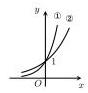
\includegraphics[max width=0.2\textwidth]{images/bo_d7fr3gc91nqc7381iccg_178_330_574_88_93_0.jpg}
\end{center}
\hspace*{3em} 

A

\begin{center}
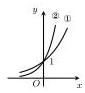
\includegraphics[max width=0.2\textwidth]{images/bo_d7fr3gc91nqc7381iccg_178_461_574_85_93_0.jpg}
\end{center}
\hspace*{3em} 

B

\begin{center}
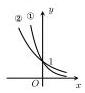
\includegraphics[max width=0.2\textwidth]{images/bo_d7fr3gc91nqc7381iccg_178_591_574_85_93_0.jpg}
\end{center}
\hspace*{3em} 

C

\begin{center}
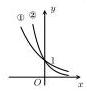
\includegraphics[max width=0.2\textwidth]{images/bo_d7fr3gc91nqc7381iccg_178_718_575_87_92_0.jpg}
\end{center}
\hspace*{3em} 

D

例 7 \(\left( {\bigstar \bigstar \text{  \ding{73}  }\text{  \ding{73}  }\text{  \ding{73}  }}\right)\)

如图所示的曲线是对数函数 \(y = {\log }_{a}x,y = {\log }_{b}x,y = {\log }_{c}x,y = {\log }_{d}x\) 的图象, 则 \(a,b,c,d\) 与 1 的大小关系为 ( )

\begin{center}
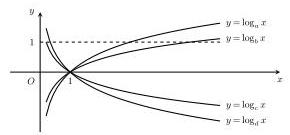
\includegraphics[max width=0.2\textwidth]{images/bo_d7fr3gc91nqc7381iccg_178_432_789_290_135_0.jpg}
\end{center}
\hspace*{3em} 

A. \(1 < d < c < a < b\) B. \(c < d < 1 < a < b\)

C. \(c < d < 1 < b < a\) D. \(d < c < 1 < a < b\)

练 7 ( \ding{72}  \ding{72}  \ding{72}  \ding{73}  \ding{73} )

已知 \(a > 0,b > 0\) ,且 \({ab} = 1,a \neq  1\) ,则函数 \(f\left( x\right)  = {a}^{x}\) 与函数 \(g\left( x\right)  =  - {\log }_{b}x\) 在

同一坐标系中的图象可能是 ( )

\begin{center}
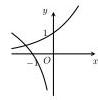
\includegraphics[max width=0.2\textwidth]{images/bo_d7fr3gc91nqc7381iccg_178_918_273_98_100_0.jpg}
\end{center}
\hspace*{3em} 

A

\begin{center}
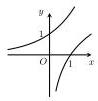
\includegraphics[max width=0.2\textwidth]{images/bo_d7fr3gc91nqc7381iccg_178_1051_272_98_101_0.jpg}
\end{center}
\hspace*{3em} 

B

\begin{center}
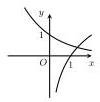
\includegraphics[max width=0.2\textwidth]{images/bo_d7fr3gc91nqc7381iccg_178_1180_271_100_102_0.jpg}
\end{center}
\hspace*{3em} 

C

\begin{center}
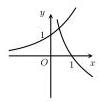
\includegraphics[max width=0.2\textwidth]{images/bo_d7fr3gc91nqc7381iccg_178_1308_271_99_102_0.jpg}
\end{center}
\hspace*{3em} 

D

例 8 \(\left( {\bigstar \bigstar \text{  \ding{73}  }\text{  \ding{73}  }\text{  \ding{73}  }}\right)\)

如图,幂函数 \(y = {x}^{a},y = {x}^{b},y = {x}^{c},y = {x}^{d}\) 在第一象限内的图象,则 \(a,b,c,d\) 的大小关系为 ( )

\begin{center}
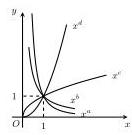
\includegraphics[max width=0.2\textwidth]{images/bo_d7fr3gc91nqc7381iccg_178_1106_491_132_135_0.jpg}
\end{center}
\hspace*{3em} 

A. \(a < b < c < d\;\) B. \(a < b < d < c\;\) C. \(b < a < c < d\;\) D. \(b < a < d < c\)

练 8 \(\left( {\phi  \star  \phi  \star  \phi  \star  \phi }\right)\)

函数 \(y = \frac{1}{x},y = x,y = 1\) 的图象和直线 \(x = 1\) 将平面直角坐标系的第一象限分为 8 个部分: \circled{1}  \circled{2}  \circled{3}  \circled{4}  \circled{5}  \circled{6}  \circled{7}  \circled{8} ，若幂函数 \(f\left( x\right)\) 的图象经过的部分是 \circled{4}  \circled{8} ，则 \(f\left( x\right)\) 可能是 ( )

\begin{center}
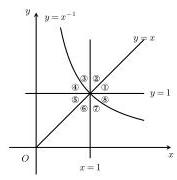
\includegraphics[max width=0.2\textwidth]{images/bo_d7fr3gc91nqc7381iccg_178_1083_784_177_180_0.jpg}
\end{center}
\hspace*{3em} 

A. \(y = {x}^{2}\) B. \(y = \frac{1}{\sqrt{x}}\) C. \(y = {x}^{\frac{1}{2}}\) D. \(y = {x}^{-2}\)

1、根据平移、对称、翻折和伸缩变换画图

例 1 已知 \(f\left( x\right)  = \ln x\) ,画出下列函数的图象

(1) \(y = f\left( {x - 1}\right)\) (2) \(y = f\left( x\right)  + 1\) (3) \(y = f\left( {-x}\right)\)

(4) \(y =  - f\left( x\right)\) (5) \(y = \left| {f\left( x\right) }\right|\) (6) \(y = f\left( \left| x\right| \right)\)

(1)

\begin{center}
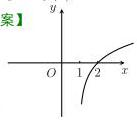
\includegraphics[max width=0.2\textwidth]{images/bo_d7fr3gc91nqc7381iccg_178_334_1250_137_122_0.jpg}
\end{center}
\hspace*{3em} 

(2)

\begin{center}
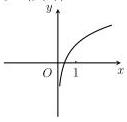
\includegraphics[max width=0.2\textwidth]{images/bo_d7fr3gc91nqc7381iccg_178_517_1250_127_122_0.jpg}
\end{center}
\hspace*{3em} 

(3)

\begin{center}
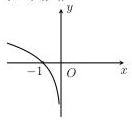
\includegraphics[max width=0.2\textwidth]{images/bo_d7fr3gc91nqc7381iccg_178_693_1250_132_121_0.jpg}
\end{center}
\hspace*{3em} 

(4)

\begin{center}
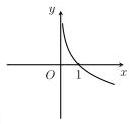
\includegraphics[max width=0.2\textwidth]{images/bo_d7fr3gc91nqc7381iccg_178_335_1377_130_124_0.jpg}
\end{center}
\hspace*{3em} 

(5)

\begin{center}
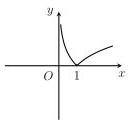
\includegraphics[max width=0.2\textwidth]{images/bo_d7fr3gc91nqc7381iccg_178_516_1376_129_126_0.jpg}
\end{center}
\hspace*{3em} 

(6)

\begin{center}
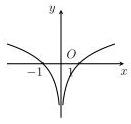
\includegraphics[max width=0.2\textwidth]{images/bo_d7fr3gc91nqc7381iccg_178_693_1378_131_124_0.jpg}
\end{center}
\hspace*{3em} 

练 1 画出下列函数的图象

(1) \(y = {2}^{x + 1} - 1\)

(4) \(y = \frac{x - 1}{x + 1}\)

(2) \(y = {2}^{-\left| x\right| }\)

(5) \(y = \frac{{2x} + 1}{x - 1}\)

(3) \(y = \left| {{2}^{\left| x\right| } - 2}\right|\)

(6) \(y = \left| {x + 1}\right|\)

【答案】

\begin{center}
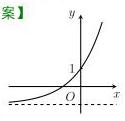
\includegraphics[max width=0.2\textwidth]{images/bo_d7fr3gc91nqc7381iccg_178_333_1598_125_121_0.jpg}
\end{center}
\hspace*{3em} 

(1)

(2)

\begin{center}
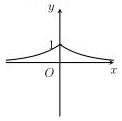
\includegraphics[max width=0.2\textwidth]{images/bo_d7fr3gc91nqc7381iccg_178_515_1595_122_121_0.jpg}
\end{center}
\hspace*{3em} 

(3)

\begin{center}
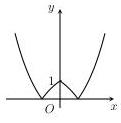
\includegraphics[max width=0.2\textwidth]{images/bo_d7fr3gc91nqc7381iccg_178_694_1594_121_123_0.jpg}
\end{center}
\hspace*{3em} 

(4)

\begin{center}
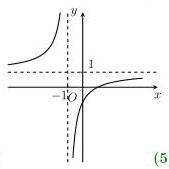
\includegraphics[max width=0.2\textwidth]{images/bo_d7fr3gc91nqc7381iccg_178_334_1721_169_169_0.jpg}
\end{center}
\hspace*{3em} 

\begin{center}
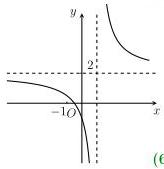
\includegraphics[max width=0.2\textwidth]{images/bo_d7fr3gc91nqc7381iccg_178_514_1720_164_169_0.jpg}
\end{center}
\hspace*{3em} 

\begin{center}
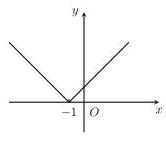
\includegraphics[max width=0.2\textwidth]{images/bo_d7fr3gc91nqc7381iccg_178_691_1751_166_141_0.jpg}
\end{center}
\hspace*{3em} 

\section*{2、根据函数的性质画图}

例 2 画出下列函数的图象

(1)

\begin{center}
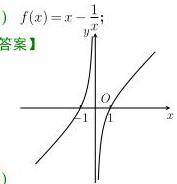
\includegraphics[max width=0.2\textwidth]{images/bo_d7fr3gc91nqc7381iccg_178_923_1196_177_184_0.jpg}
\end{center}
\hspace*{3em} 

(2) \(f\left( x\right)  = x + \ln x\) ;

(2)

\begin{center}
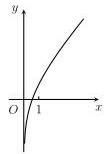
\includegraphics[max width=0.2\textwidth]{images/bo_d7fr3gc91nqc7381iccg_178_1208_1227_104_154_0.jpg}
\end{center}
\hspace*{3em} 

练 2 已知奇函数 \(f\left( x\right)\) 定义域为 \(\mathbf{R}\) ,当 \(x \in  \left\lbrack  {0,1}\right\rbrack\) 时, \(f\left( x\right)  = x\) ,且 \(f\left( x\right)\) 的图象关于 \(x = 1\) 对称,画出 \(f\left( x\right)\) 在 \(\left\lbrack  {-5,5}\right\rbrack\) 的函数图象.

【答案】

\begin{center}
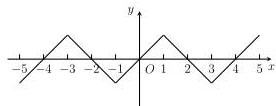
\includegraphics[max width=0.2\textwidth]{images/bo_d7fr3gc91nqc7381iccg_178_964_1462_276_106_0.jpg}
\end{center}
\hspace*{3em} 

\section*{3、复杂函数运用导数画图}

例 3 画出下列函数的图象

\begin{center}
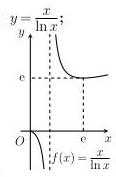
\includegraphics[max width=0.2\textwidth]{images/bo_d7fr3gc91nqc7381iccg_178_1291_1620_116_177_0.jpg}
\end{center}
\hspace*{3em} 

(1) \(y = x\ln x\)

(2) \(y = \frac{\ln x}{x}\)

\begin{center}
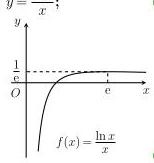
\includegraphics[max width=0.2\textwidth]{images/bo_d7fr3gc91nqc7381iccg_178_1116_1636_154_163_0.jpg}
\end{center}
\hspace*{3em} 

(3)

(3)

\begin{center}
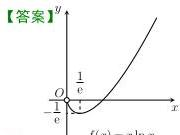
\includegraphics[max width=0.2\textwidth]{images/bo_d7fr3gc91nqc7381iccg_178_905_1648_180_135_0.jpg}
\end{center}
\hspace*{3em} 

\(f\left( x\right)  = x\ln x\)

(2) (1)

1. 图的细节均可直接修改, 整体效果与文档本身浑然一体.

2. 选项可以根据图的大小, 自动排列一行四个或两个或一个, 图可以居中、居右或居左.

\section*{三、课程简介与学习流程}

目前全部课程大约有 40 课时的视频，包括四方面内容，分别为:试卷编辑基础模块、讲义编辑提高模块、画图模版、幻灯片制作模版. 除此之外, 也会将学员经常遇到的问题解答制作成视频上传, 90\% 的老师都可以根据视频学习掌握, 对于在学习中有疑惑的地方, 还会提供答疑, 远程协助解决问题, 确保参与课程的学员完成学习目标, 能够独立编辑出试卷、讲义等文档. 课程目标与教学内容见附件.

\section*{课程形式}

课程包括视频课程、文档资料和若干次答疑, 其中视频课程为在线视频, 可以回放, 老师们可以根据自己的时间安排学习, 同时参考提供的文档资料, 对于有疑问的地方, 会通过微信或者远程提供答疑, 这样的教学方式,符合学习规律,节约时间,效率高,比自学节约 90\% 的时间,参加课程快则一天，慢则一周即可独立排版一份试卷、讲义。

\section*{电脑基础}

学习软件所需要的电脑基础:会打字，大多数情况能够打字不看键盘。 课程是面向零基础的中学老师, 不需要额外的编程基础.

\section*{学习流程}

1. 报名参加课程、安装软件、配置软件, 浏览课程所发资料, 知道资料都有哪些内容;

2. 认真观看前五个视频, 认真操作;

3. 尝试排版一份高考试卷, 遇到问题, 先查看视频和代码手册, 如果不能解决, 微信联系我即可.

4. 后期根据自己需求, 选择性的学习视频课程.

未尽事宜，可微信交流.

\section*{附件: 公式效果}

基本符号

希腊字母

集合

\begin{center}
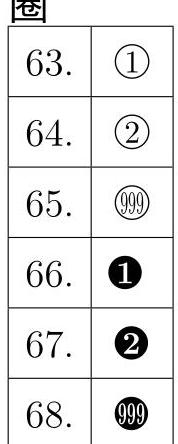
\includegraphics[max width=0.2\textwidth]{images/bo_d7fr3gc91nqc7381iccg_180_1068_1473_178_444_0.jpg}
\end{center}
\hspace*{3em} 

\begin{center}
\adjustbox{max width=\textwidth}{
\begin{tabular}{|c|c|c|}
\hline
\phantom{X} & 序号 & 符号 \\
\cline{1-3}
\phantom{X} & 1. & \(\sqrt{2},\sqrt[3]{3},\sqrt{\frac{1}{2}}\) \\
\cline{1-3}
\phantom{X} & 2. & \(\frac{2}{3},\frac{\sqrt{3}}{2}\) \\
\cline{1-3}
\phantom{X} & 3. & \(\overrightarrow{AB},\mathbf{a}\) \\
\cline{1-3}
\phantom{X} & 4. & \(\bar{a},\widehat{a},\overline{1234}\) \\
\cline{1-3}
\phantom{X} & 5. & \({a}_{m},{a}^{n},{a}_{n + 1}^{n + 2}\) \\
\cline{1-3}
\phantom{X} & 6. & \{\} \\
\cline{1-3}
\phantom{X} & 7. & \% \\
\cline{1-3}
\phantom{X} & 8. & \(+ \infty , - \infty\) \\
\cline{1-3}
\phantom{X} & 9. & \(\because \therefore\) \\
\cline{1-3}
\phantom{X} & 10. & \(\langle \mathbf{a},\mathbf{b}\rangle\) \\
\cline{1-3}
\phantom{X} & 11. & \(\int\) \\
\cline{1-3}
\phantom{X} & 12. &  \ding{56}  \\
\cline{1-3}
\phantom{X} & 13. & ÷ \\
\cline{1-3}
\phantom{X} & 14. & + \\
\cline{1-3}
\phantom{X} & 15. & < \\
\cline{1-3}
\phantom{X} & 16. & 之 \\
\cline{1-3}
\phantom{X} & 17. & \(\neq\) \\
\cline{1-3}
\phantom{X} & 18. & \(\approx\) \\
\cline{1-3}
\phantom{X} & 19. & ... \\
\cline{1-3}
\phantom{X} & 20. & 十 \\
\cline{1-3}
\phantom{X} & 21. & (mod \(m\) ) \\
\cline{1-3}
\phantom{X} & 22. & 着重号 \\
\cline{1-3}
\phantom{X} & 23. & 公式中中文 \\
\cline{1-3}
\phantom{X} & 24. & 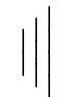
\includegraphics[max width=0.2\textwidth]{images/bo_d7fr3gc91nqc7381iccg_180_383_2030_60_97_0.jpg} \\
\cline{1-3}
\hline
\end{tabular}
}
\end{center}

\begin{center}
\adjustbox{max width=\textwidth}{
\begin{tabular}{|c|c|c|}
\hline
\phantom{X} & 序号 & 符号 \\
\cline{1-3}
\phantom{X} & 25. & \(\alpha\) \\
\cline{1-3}
\phantom{X} & 26. & \(\beta\) \\
\cline{1-3}
\phantom{X} & 27. & \(\gamma\) \\
\cline{1-3}
\phantom{X} & 28. & \(\delta\) \\
\cline{1-3}
\phantom{X} & 29. & \(\varepsilon\) \\
\cline{1-3}
\phantom{X} & 30. & \(\eta\) \\
\cline{1-3}
\phantom{X} & 31. & \(\theta\) \\
\cline{1-3}
\phantom{X} & 32. & \(\lambda\) \\
\cline{1-3}
\phantom{X} & 33. & \(\mu\) \\
\cline{1-3}
\phantom{X} & 34. & \(\nu\) \\
\cline{1-3}
\phantom{X} & 35. & \(\xi\) \\
\cline{1-3}
\phantom{X} & 36. & \(\pi\) \\
\cline{1-3}
\phantom{X} & 37. & \(\rho\) \\
\cline{1-3}
\phantom{X} & 38. & \(\sigma\) \\
\cline{1-3}
\phantom{X} & 39. & \(\varphi\) \\
\cline{1-3}
\phantom{X} & 40. & \(\omega\) \\
\cline{1-3}
\phantom{X} & 41. & \(\Delta\) \\
\cline{1-3}
\phantom{X} & 42. & \(\Omega\) \\
\cline{1-3}
\phantom{X} & 43. & \(\Gamma\) \\
\cline{1-3}
\hline
\end{tabular}
}
\end{center}

\begin{center}
\adjustbox{max width=\textwidth}{
\begin{tabular}{|c|c|}
\hline
序号 & 符号 \\
\cline{1-2}
48. & UU \\
\cline{1-2}
49. & \(\cap   \cap\) \\
\cline{1-2}
50. & 三 \\
\cline{1-2}
51. & 三 \\
\cline{1-2}
52. & 字 \\
\cline{1-2}
53. & \({\complement }_{U}A\) \\
\cline{1-2}
54. & \(\in   \notin\) \\
\cline{1-2}
55. & \(\varnothing\) \\
\cline{1-2}
56. & \(\otimes\) \\
\cline{1-2}
57. & \(\oplus\) \\
\cline{1-2}
58. & ※ \\
\cline{1-2}
59. & \(\neg p\) \\
\cline{1-2}
60. & \(p \vee  q\) \\
\cline{1-2}
61. & \(p \land  q\) \\
\cline{1-2}
62. & \(\exists \forall\) \\
\cline{1-2}
\hline
\end{tabular}
}
\end{center}

卷

\begin{center}
\adjustbox{max width=\textwidth}{
\begin{tabular}{|c|c|c|c|}
\hline
\multicolumn{4}{|c|}{大型运算符号} \\
\cline{1-4}
\phantom{X} & 44. & \(\mathop{\sum }\limits_{{i = 1}}^{n}\) & \phantom{X} \\
\cline{1-4}
\phantom{X} & 45. & \(\mathop{\prod }\limits_{{i = 1}}^{n}\) & \phantom{X} \\
\cline{1-4}
\phantom{X} & 46. & \({\int }_{1}^{n}\) & \phantom{X} \\
\cline{1-4}
\phantom{X} & 47. & \makecell{ lim \\ \(x \rightarrow   + \infty\) } & \phantom{X} \\
\cline{1-4}
\hline
\end{tabular}
}
\end{center}

判断对错

\begin{center}
\adjustbox{max width=\textwidth}{
\begin{tabular}{|c|c|}
\hline
69. & \phantom{X} \\
\cline{1-2}
70. & \phantom{X} \\
\cline{1-2}
\hline
\end{tabular}
}
\end{center}

几何

\begin{center}
\adjustbox{max width=\textwidth}{
\begin{tabular}{|c|c|}
\hline
序号 & 符号 \\
\cline{1-2}
71. & ⊥ \\
\cline{1-2}
72. & 丨 \\
\cline{1-2}
73. & \(\bigtriangleup\) \\
\cline{1-2}
74. &  \circled{2}  \\
\cline{1-2}
75. & L \\
\cline{1-2}
76. & \(□\) \\
\cline{1-2}
77. & // \\
\cline{1-2}
78. & ～ \\
\cline{1-2}
79. & 了 \\
\cline{1-2}
80. & ≅ \\
\cline{1-2}
81. & 19 \\
\cline{1-2}
82. & \(\overset{\text{ ⏜ }}{AB}\) \\
\cline{1-2}
\hline
\end{tabular}
}
\end{center}

难度选择填空

\[
f\left( x\right)  = \left\{  {\begin{array}{l} {x}^{2} - {2x} + 3,x \leq  1, \\  x - 2,x > 1, \end{array}\;f\left( x\right)  = \left\{  \begin{array}{ll} {x}^{2} - {2x} + 3, & x \leq  1, \\  x - 2, & x > 1, \end{array}\right. }\right.
\]

\begin{center}
\adjustbox{max width=\textwidth}{
\begin{tabular}{|c|c|c|}
\hline
\phantom{X} & 83. &  \ding{72}  \ding{73}  \ding{73}  \ding{73}  \ding{73}  \\
\cline{1-3}
\phantom{X} & 84. &  \ding{72}  \ding{72}  \ding{73}  \ding{73}  \ding{73}  \\
\cline{1-3}
\phantom{X} & 85. &  \ding{72}  \ding{72}  \ding{72}  \ding{73}  \ding{73}  \\
\cline{1-3}
\phantom{X} & 86. &  \ding{72}  \ding{72}  \ding{72}  \ding{72}  \ding{73}  \\
\cline{1-3}
\phantom{X} & 87. &  \ding{72}  \ding{72}  \ding{72}  \ding{72}  \ding{72}  \\
\cline{1-3}
\phantom{X} & 88. &  \ding{73}  \ding{73}  \ding{73}  \ding{73}  \ding{73}  \\
\cline{1-3}
\phantom{X} & 89. &  \ding{72}  \ding{72}  \ding{72}  \ding{73}  \ding{73}  \\
\cline{1-3}
\phantom{X} & 90. & ( ) \\
\cline{1-3}
\phantom{X} & 91. & \_\_\_\_\_ \\
\cline{1-3}
\phantom{X} & 92. & \_\_\_\_\_ \\
\cline{1-3}
\hline
\end{tabular}
}
\end{center}

\begin{center}
\adjustbox{max width=\textwidth}{
\begin{tabular}{|c|c|c|}
\hline
\multicolumn{3}{|c|}{函数} \\
\cline{1-3}
\multirow{13}{*}{\phantom{X}} & 序号 & 符号 \\
\cline{2-3}
 & 93. & \(\lim x\) \\
\cline{2-3}
 & 94. & \(\cos x\) \\
\cline{2-3}
 & 95. & \(\sin x\) \\
\cline{2-3}
 & 96. & \(\tan x\) \\
\cline{2-3}
 & 97. & \(\lg x\) \\
\cline{2-3}
 & 98. & \(\ln x\) \\
\cline{2-3}
 & 99. & \(\log x\) \\
\cline{2-3}
 & 100. & \(\max x\) \\
\cline{2-3}
 & 101. & \(\min x\) \\
\cline{2-3}
 & 102. & \(\arccos x\) \\
\cline{2-3}
 & 103. & \(\arcsin x\) \\
\cline{2-3}
 & 104. & \(\arctan x\) \\
\cline{1-3}
\hline
\end{tabular}
}
\end{center}

罗马数字

105. I

106. II

107. III

108. X

109. XV

110. i

111. ii

112. iii

113. X

114. XV

\begin{center}
\adjustbox{max width=\textwidth}{
\begin{tabular}{|c|c|}
\hline
\multicolumn{2}{|c|}{箭头} \\
\cline{1-2}
115. &  \ding{51}  \\
\cline{1-2}
116. & \(\rightarrow\) \\
\cline{1-2}
117. & \(\Leftarrow\) \\
\cline{1-2}
118. & \(\Rightarrow\) \\
\cline{1-2}
119. & ⇔ \\
\cline{1-2}
120. & 今 \\
\cline{1-2}
121. & ↗ \\
\cline{1-2}
122. & ↘ \\
\cline{1-2}
123. & 应 \\
\cline{1-2}
124. &  \ding{51}  \\
\cline{1-2}
125. & \(\uparrow   \downarrow\) \\
\cline{1-2}
126. &  \ding{51}  \\
\cline{1-2}
127. & 一 \\
\cline{1-2}
128. & 一 \\
\cline{1-2}
129. & 一 \\
\cline{1-2}
130. & \(\Rightarrow\) \\
\cline{1-2}
131. & \(\Leftrightarrow\) \\
\cline{1-2}
132. & 上 \\
\cline{1-2}
133. & 上 \\
\cline{1-2}
134. & 占 \\
\cline{1-2}
135. & 二 \\
\cline{1-2}
\hline
\end{tabular}
}
\end{center}

\section*{公式等号对齐}

\({10} = 1 + 9\)

\[
{10} = 1 + 9
\]

\({10} = 1 + 1 + 8 \; {10} = 1 + 1 + 8\)

\({10} = 1 + 1 + 1 + 7 \; {10} = 1 + 1 + 1 + 7\)

在我们教学、做题的过程中, 有很多好的想法、思路, 但由于没有及时的记录、整理，而逐渐遗忘，即使努力回想，多是徒劳，非常遗憾. 学会 IATEX, 可以方程方便的编辑公式, 画图, 大大提高效率记录我们专业成长的每一步，让每个灵感闪现的时刻不再转瞬即逝！

给大家提供一个决策的角度:一件事是否值得做，当下可能觉得受很多因素影响, 不知道如何取舍的时, 不妨让五年、十年后的自己帮做决策, 十年之后哪些因素才是最重要的, 立刻变得清晰.

一项技能会在时间的作用下, 愈发珍贵, IATEX 这一工具, 方便记录, 平时的积累够了，关键时刻就能迸发无穷的力量，一起加入学习吧.

\section*{一、函数图象}

\begin{center}
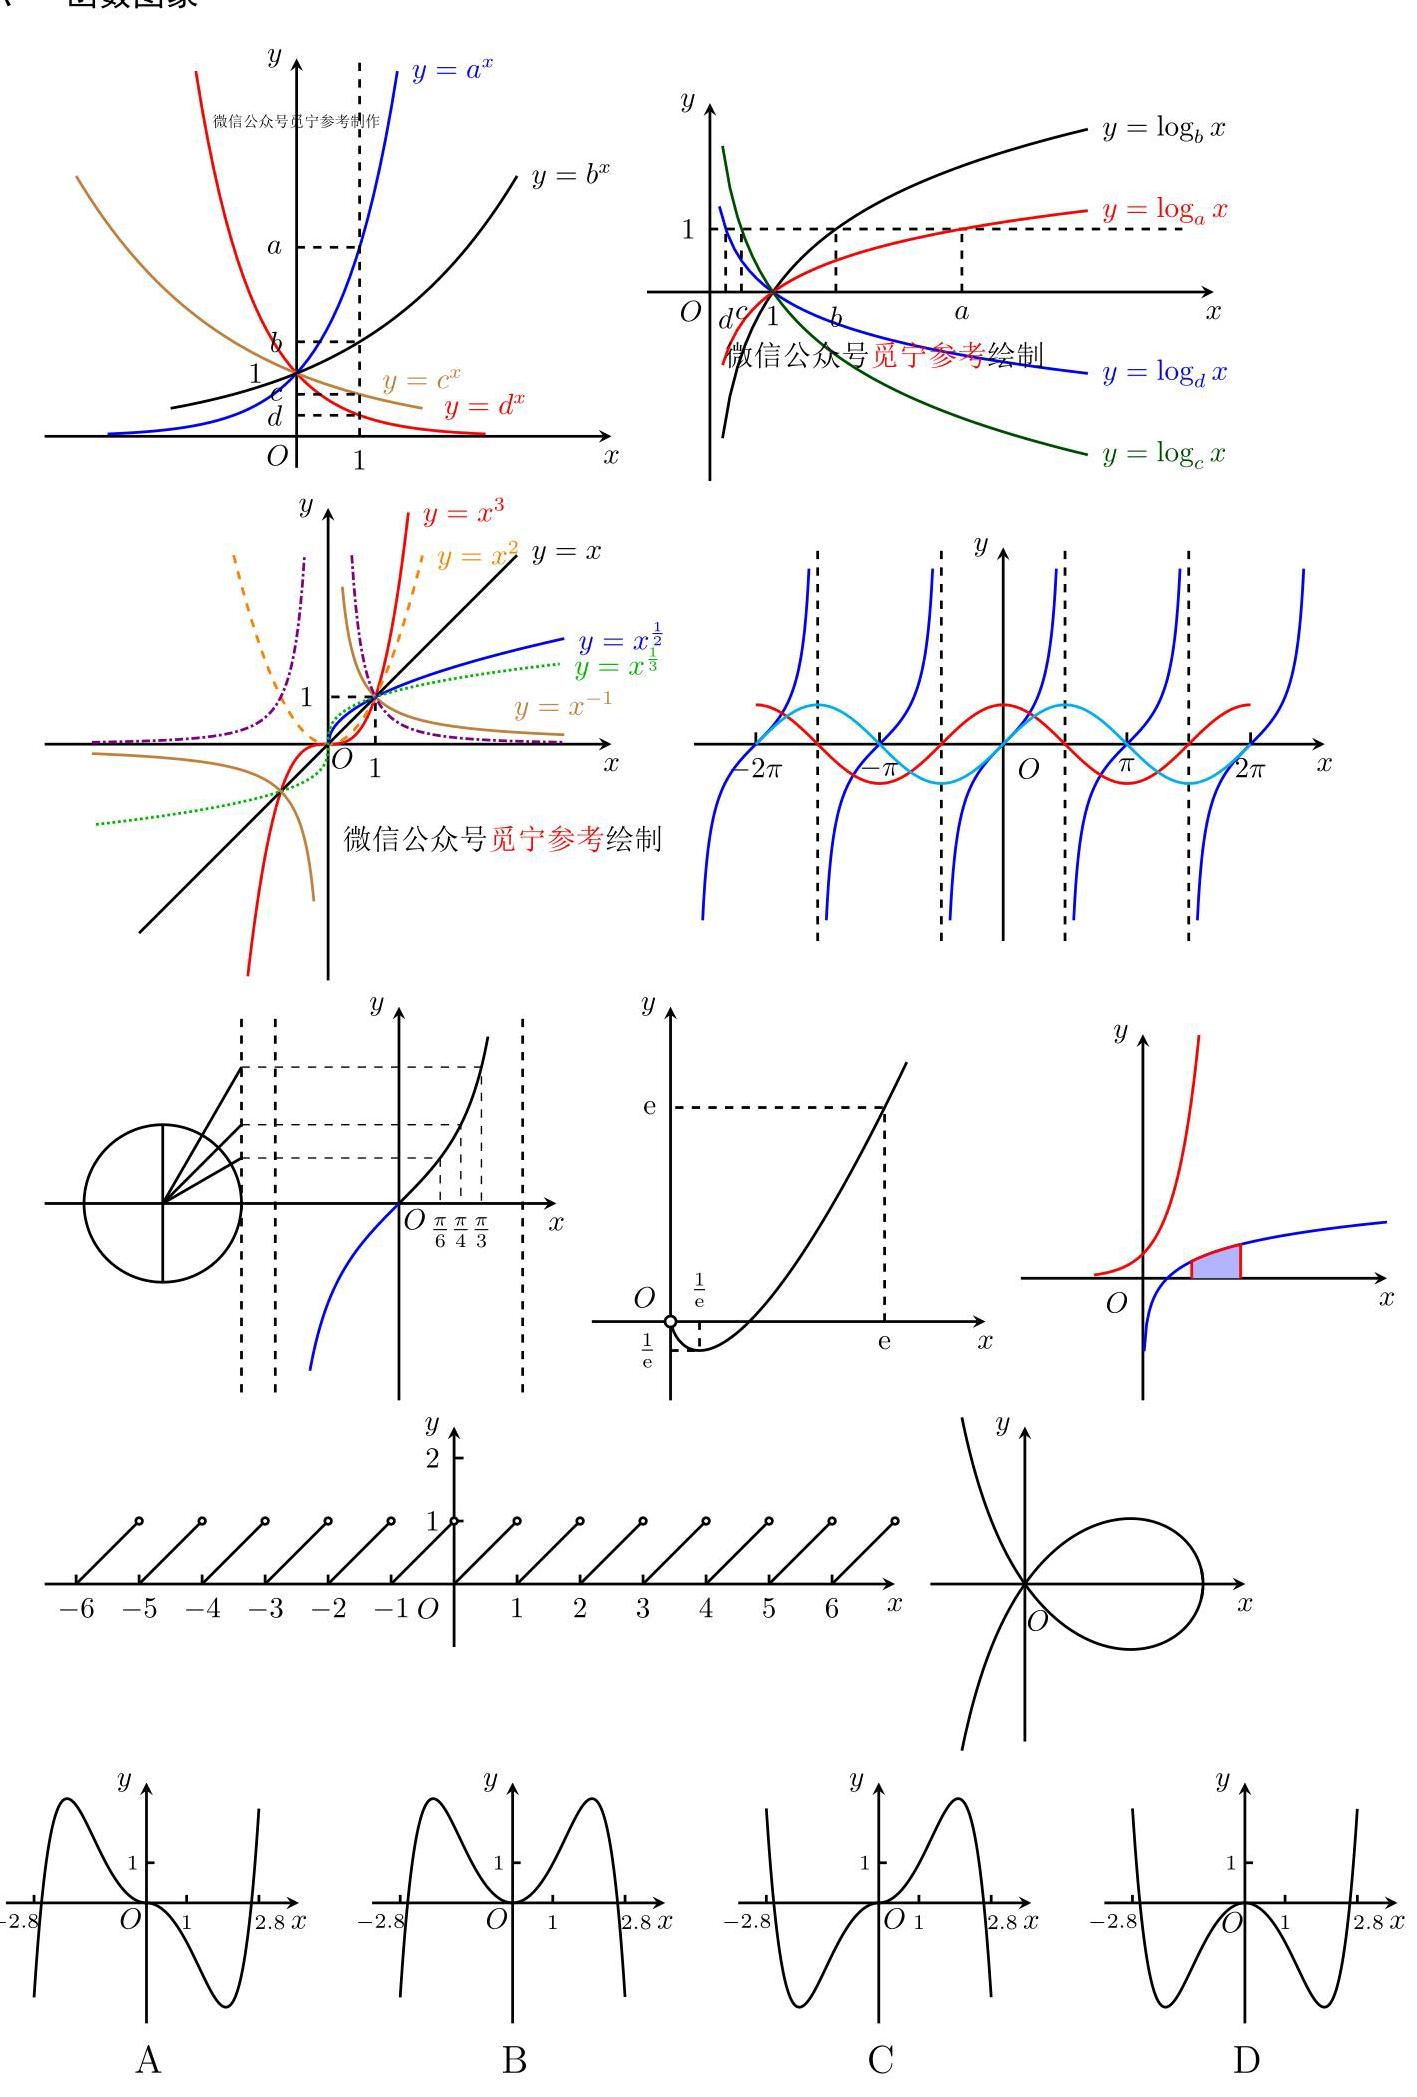
\includegraphics[max width=1.0\textwidth]{images/bo_d7fr3gc91nqc7381iccg_183_129_129_1417_2097_0.jpg}
\end{center}
\hspace*{3em} 

关注微信公众号《觅宁参考》免费下载上述画图软件，添加小编微信，学习公式编辑、画图、下载高中数学专题第 1 页 共 4 页

\section*{二、立体几何}

\begin{center}
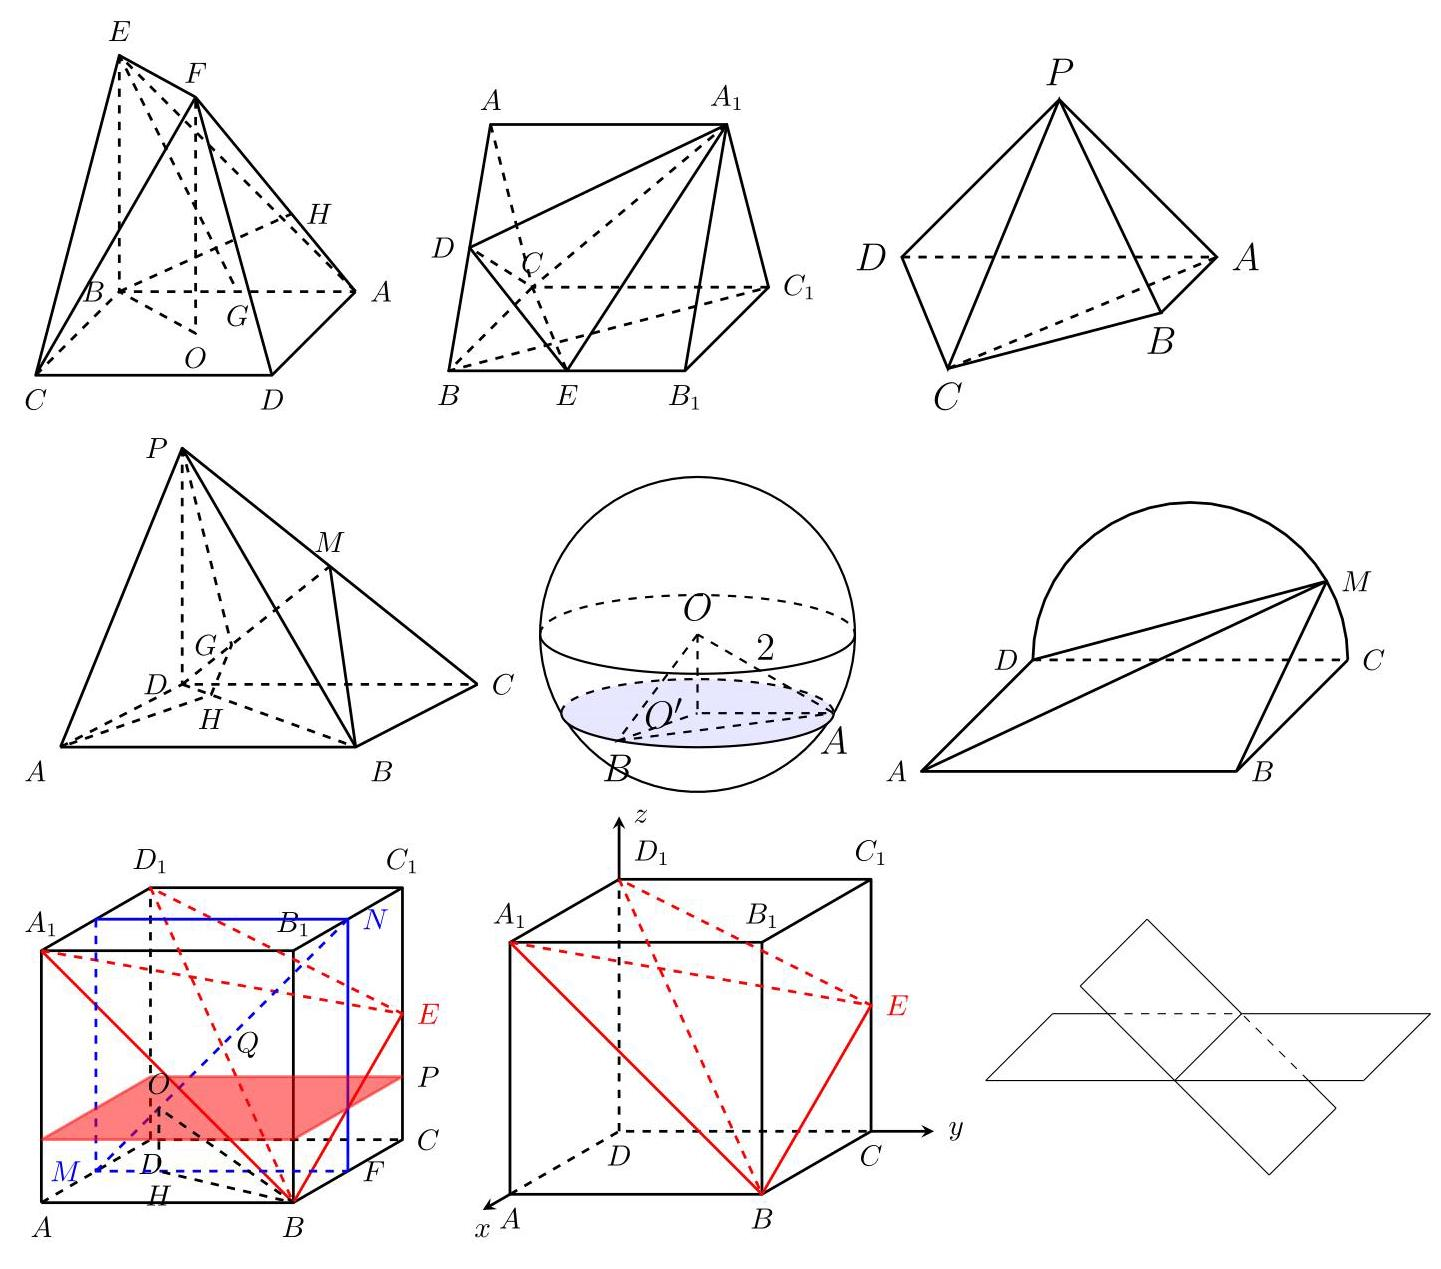
\includegraphics[max width=1.0\textwidth]{images/bo_d7fr3gc91nqc7381iccg_184_161_157_1441_1269_0.jpg}
\end{center}
\hspace*{3em} 

\section*{三、统计图}

\begin{center}
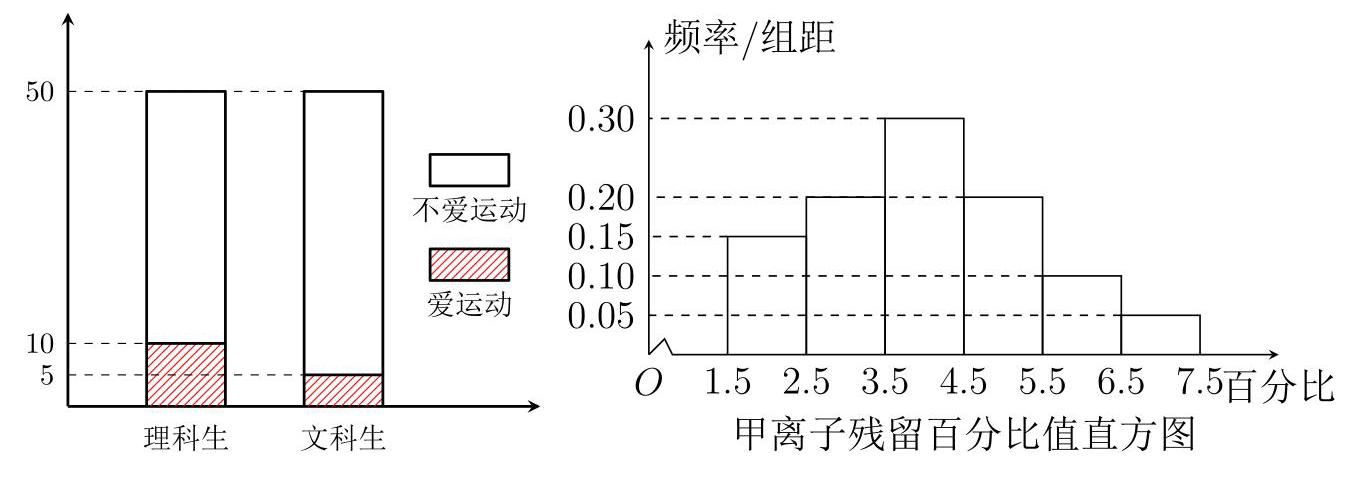
\includegraphics[max width=1.0\textwidth]{images/bo_d7fr3gc91nqc7381iccg_184_160_1539_1372_478_0.jpg}
\end{center}
\hspace*{3em} 

关注微信公众号《觅宁参考》免费下载上述画图软件，添加小编微信，学习公式编辑、画图、下载高中数学专题

第 2 页 共 4 页

\begin{center}
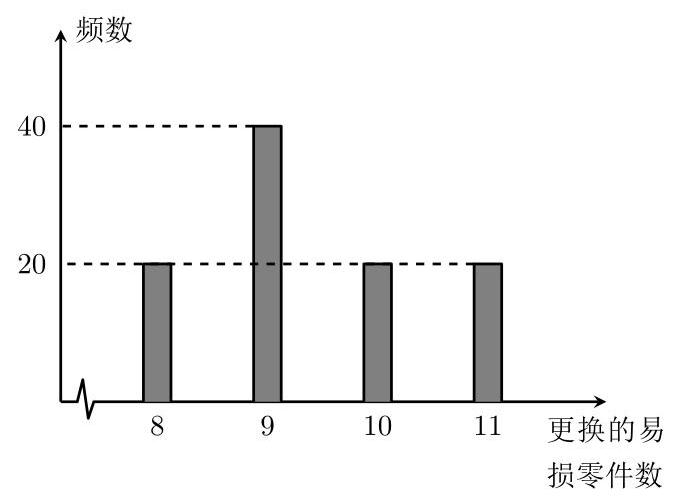
\includegraphics[max width=0.5\textwidth]{images/bo_d7fr3gc91nqc7381iccg_185_168_103_677_501_0.jpg}
\end{center}
\hspace*{3em} 

第三产业收入

28\%

种植收入 37\%

5\% 其他收入

30\% 养殖收入

建设后经济收入构成比例

四、圆锥曲线等平面图

\begin{center}
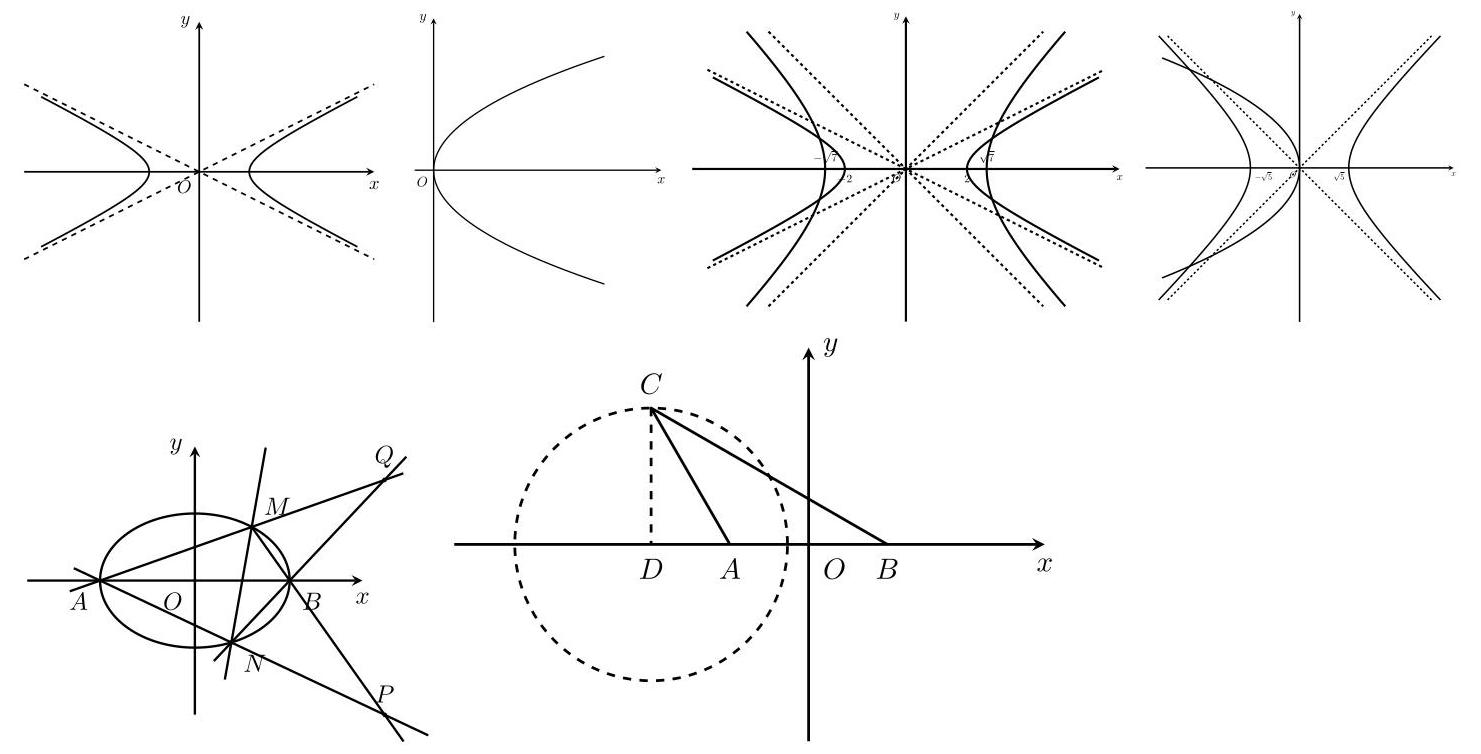
\includegraphics[max width=1.0\textwidth]{images/bo_d7fr3gc91nqc7381iccg_185_157_735_1481_754_0.jpg}
\end{center}
\hspace*{3em} 

\section*{五、 其他平面图形}

\begin{center}
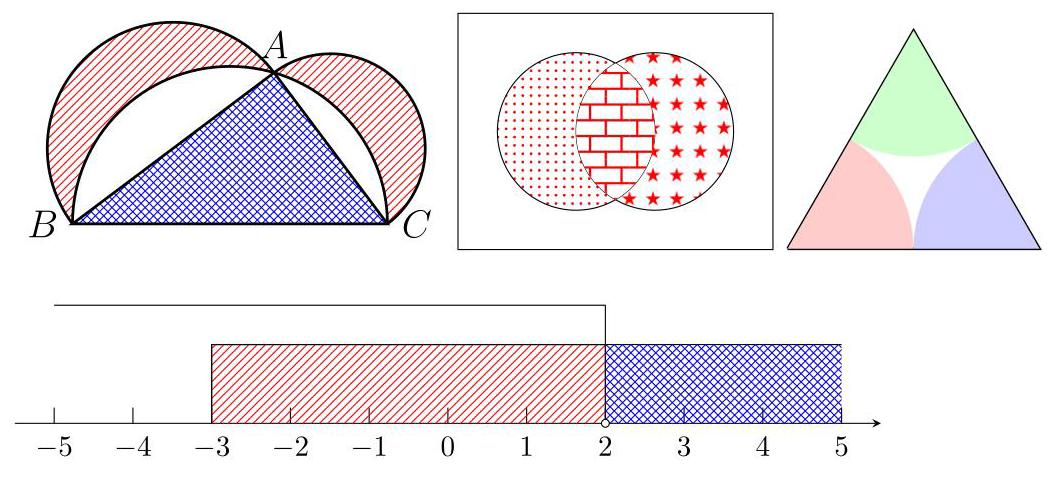
\includegraphics[max width=0.9\textwidth]{images/bo_d7fr3gc91nqc7381iccg_185_158_1612_1057_478_0.jpg}
\end{center}
\hspace*{3em} 

关注微信公众号《觅宁参考》免费下载上述画图软件，添加小编微信，学习公式编辑、画图、下载高中数学专题第 3 页 共 4 页

\section*{六、其它图形}

\begin{center}
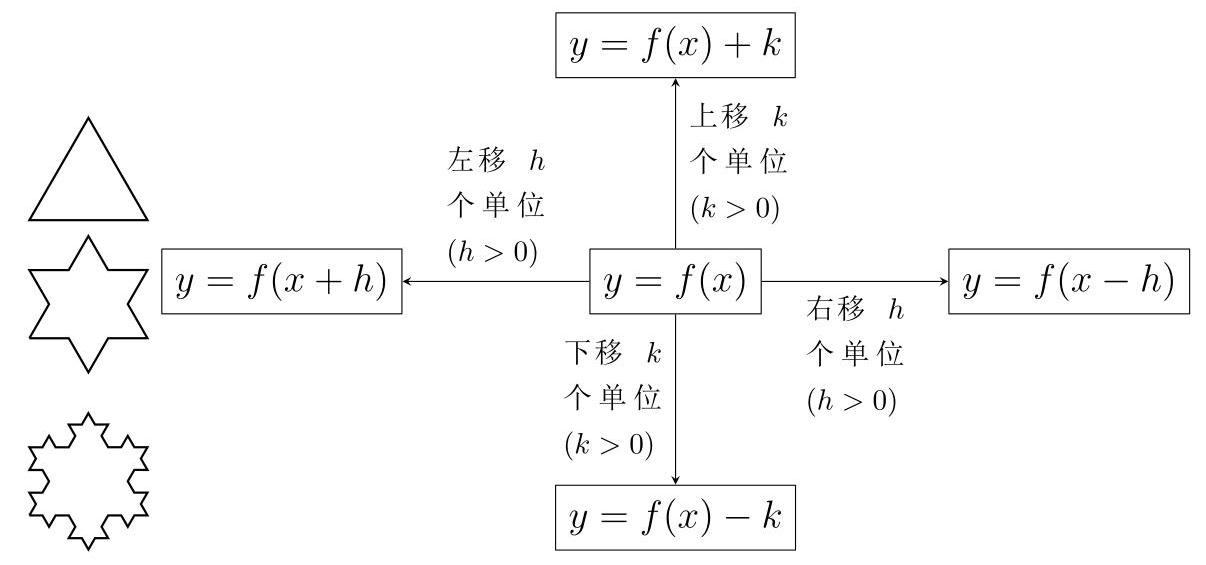
\includegraphics[max width=1.0\textwidth]{images/bo_d7fr3gc91nqc7381iccg_186_144_153_1206_565_0.jpg}
\end{center}
\hspace*{3em} 

七、三视图

\begin{center}
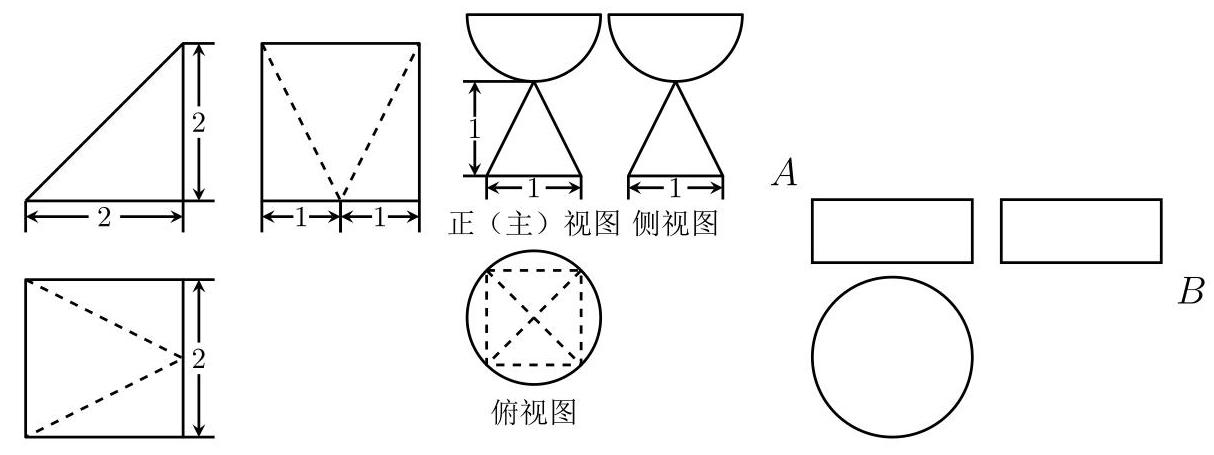
\includegraphics[max width=1.0\textwidth]{images/bo_d7fr3gc91nqc7381iccg_186_148_826_1214_455_0.jpg}
\end{center}
\hspace*{3em} 

\section*{八、流程图}

\begin{center}
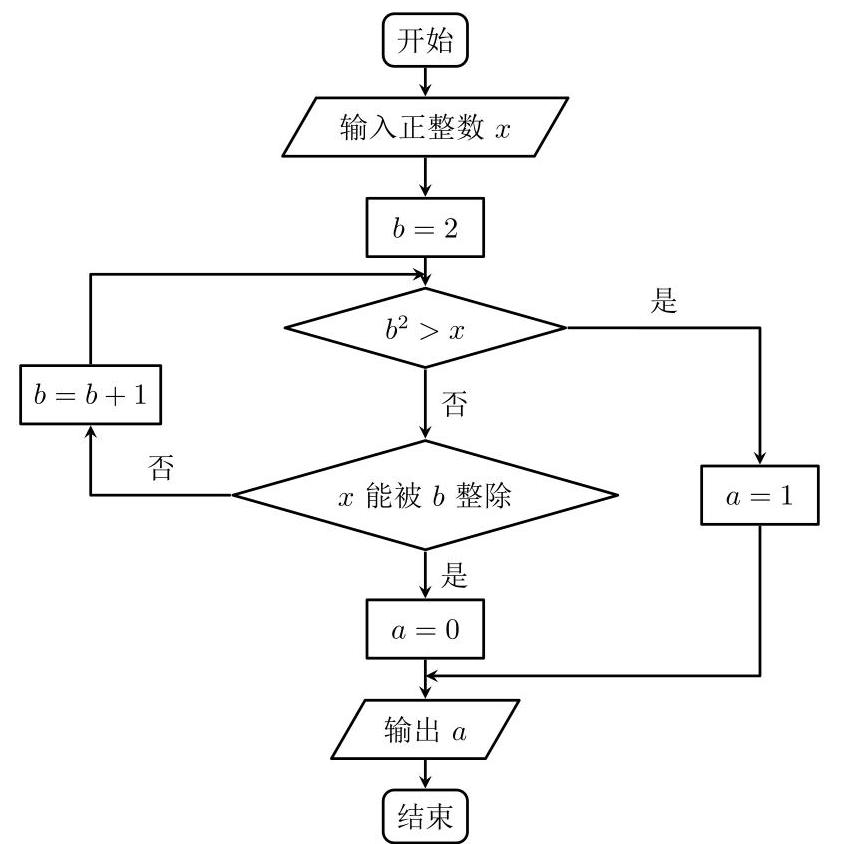
\includegraphics[max width=0.7\textwidth]{images/bo_d7fr3gc91nqc7381iccg_186_153_1388_841_844_0.jpg}
\end{center}
\hspace*{3em} 

关注微信公众号《觅宁参考》免费下载上述画图软件，添加小编微信，学习公式编辑、画图、下载高中数学专题第 4 页 共 4 页

\section*{指对幂图象及其性质}

\section*{一、指对幂的函数图象}

例 1 已知 \({y}_{1} = {\left( \frac{1}{3}\right) }^{x},{y}_{2} = {3}^{x},{y}_{3} = {10}^{-x},{y}_{4} = {10}^{x}\) ,则在同一直角坐标系内,他们的图象为 ( )

\begin{center}
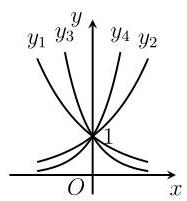
\includegraphics[max width=0.2\textwidth]{images/bo_d7fr3gc91nqc7381iccg_187_186_296_187_201_0.jpg}
\end{center}
\hspace*{3em} 

A

\begin{center}
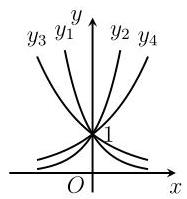
\includegraphics[max width=0.2\textwidth]{images/bo_d7fr3gc91nqc7381iccg_187_449_298_187_199_0.jpg}
\end{center}
\hspace*{3em} 

B

\begin{center}
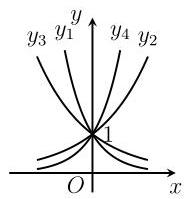
\includegraphics[max width=0.2\textwidth]{images/bo_d7fr3gc91nqc7381iccg_187_712_298_187_199_0.jpg}
\end{center}
\hspace*{3em} 

C

\begin{center}
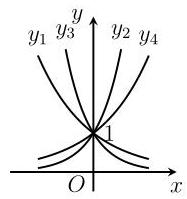
\includegraphics[max width=0.2\textwidth]{images/bo_d7fr3gc91nqc7381iccg_187_974_299_187_199_0.jpg}
\end{center}
\hspace*{3em} 

D

练 1 已知 \(0 < m < n < 1\) ,则指数函数 \(\text{  \circled{1}  }y = {m}^{x},\text{  \circled{2}  }y = {n}^{x}\) 的图象是 ( )

\begin{center}
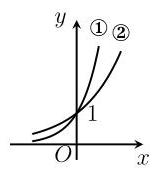
\includegraphics[max width=0.2\textwidth]{images/bo_d7fr3gc91nqc7381iccg_187_202_688_155_169_0.jpg}
\end{center}
\hspace*{3em} 

A

\begin{center}
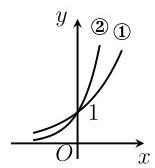
\includegraphics[max width=0.2\textwidth]{images/bo_d7fr3gc91nqc7381iccg_187_464_689_155_168_0.jpg}
\end{center}
\hspace*{3em} 

B

\begin{center}
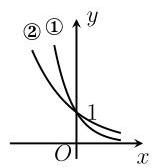
\includegraphics[max width=0.2\textwidth]{images/bo_d7fr3gc91nqc7381iccg_187_728_689_154_168_0.jpg}
\end{center}
\hspace*{3em} 

C

\begin{center}
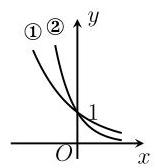
\includegraphics[max width=0.2\textwidth]{images/bo_d7fr3gc91nqc7381iccg_187_990_689_155_168_0.jpg}
\end{center}
\hspace*{3em} 

D

例 2 如图所示的曲线是对数函数 \(y = {\log }_{a}x,y = {\log }_{b}x,y = {\log }_{c}x,y = {\log }_{d}x\) 的图象,则 \(a,b,c,d\) 与 1 的大小关系为 ( )

\begin{center}
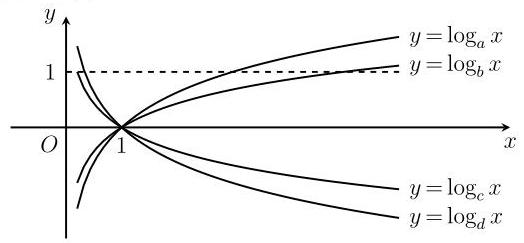
\includegraphics[max width=0.3\textwidth]{images/bo_d7fr3gc91nqc7381iccg_187_377_1093_524_243_0.jpg}
\end{center}
\hspace*{3em} 

A. \(1 < d < c < a < b\) B. \(c < d < 1 < a < b\) C. \(c < d < 1 < b < a\) D. \(d < c < 1 < a < b\)

练 2 已知 \(a > 0,b > 0\) ,且 \({ab} = 1,a \neq  1\) ,则函数 \(f\left( x\right)  = {a}^{x}\) 与函数 \(g\left( x\right)  =  - {\log }_{b}x\) 在同一坐标系中的图象可能是 ( )

\begin{center}
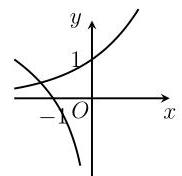
\includegraphics[max width=0.2\textwidth]{images/bo_d7fr3gc91nqc7381iccg_187_1300_176_182_176_0.jpg}
\end{center}
\hspace*{3em} 

A

\begin{center}
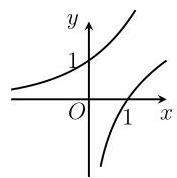
\includegraphics[max width=0.2\textwidth]{images/bo_d7fr3gc91nqc7381iccg_187_1566_175_177_178_0.jpg}
\end{center}
\hspace*{3em} 

B

\begin{center}
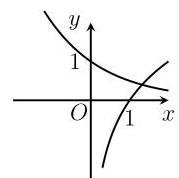
\includegraphics[max width=0.2\textwidth]{images/bo_d7fr3gc91nqc7381iccg_187_1827_174_179_178_0.jpg}
\end{center}
\hspace*{3em} 

C

\begin{center}
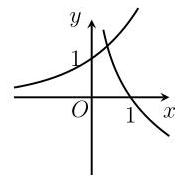
\includegraphics[max width=0.2\textwidth]{images/bo_d7fr3gc91nqc7381iccg_187_2089_177_179_176_0.jpg}
\end{center}
\hspace*{3em} 

D

\begin{center}
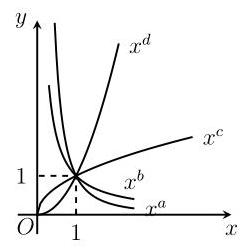
\includegraphics[max width=0.2\textwidth]{images/bo_d7fr3gc91nqc7381iccg_187_2001_545_241_248_0.jpg}
\end{center}
\hspace*{3em} 

例 3 如图,幂函数 \(y = {x}^{a},y = {x}^{b},y = {x}^{c},y = {x}^{d}\) 在第一象限内的图象,则 \(a,b,c,d\) 的大小关系为 ( )

A. \(a < b < c < d\) B. \(a < b < d < c\)

C. \(b < a < c < d\) D. \(b < a < d < c\)

\begin{center}
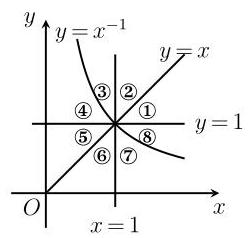
\includegraphics[max width=0.2\textwidth]{images/bo_d7fr3gc91nqc7381iccg_187_1995_909_250_238_0.jpg}
\end{center}
\hspace*{3em} 

练 3 函数 \(y = \frac{1}{x},y = x,y = 1\) 的图象和直线 \(x = 1\) 将平面直角坐标系的第一象限分为 8 个部分: \circled{1}  \circled{2}  \circled{3}  \circled{4}  \circled{5}  \circled{6}  \circled{7}  \circled{8} ，若幂函数 \(f\left( x\right)\) 的图象经过的部分是 \circled{4}  \circled{8} ，则 \(f\left( x\right)\) 可能是 ( )

A. \(y = {x}^{2}\) B. \(y = \frac{1}{\sqrt{x}}\)

C. \(y = {x}^{\frac{1}{2}}\) D. \(y = {x}^{-2}\)

\section*{1、根据平移、对称、翻折和伸缩变换画图}

例 1 已知 \(f\left( x\right)  = \ln x\) ,画出下列函数的图象

(1) \(y = f\left( {x - 1}\right)\) (2) \(y = f\left( x\right)  + 1\) (3) \(y = f\left( {-x}\right)\)

(4) \(y =  - f\left( x\right)\) (5) \(y = \left| {f\left( x\right) }\right|\) (6) \(y = f\left( \left| x\right| \right)\)

【答案】

\begin{center}
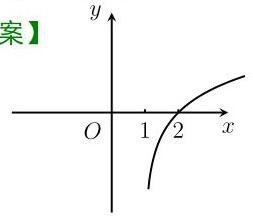
\includegraphics[max width=0.2\textwidth]{images/bo_d7fr3gc91nqc7381iccg_188_198_279_253_219_0.jpg}
\end{center}
\hspace*{3em} 

(1)

(2)

\begin{center}
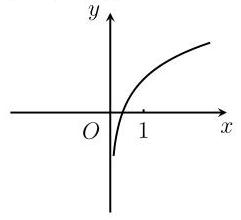
\includegraphics[max width=0.2\textwidth]{images/bo_d7fr3gc91nqc7381iccg_188_531_279_241_220_0.jpg}
\end{center}
\hspace*{3em} 

(3)

\begin{center}
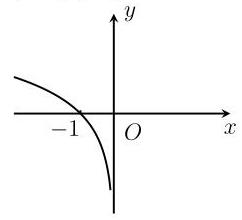
\includegraphics[max width=0.2\textwidth]{images/bo_d7fr3gc91nqc7381iccg_188_859_278_242_220_0.jpg}
\end{center}
\hspace*{3em} 

(4)

\begin{center}
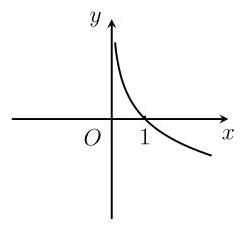
\includegraphics[max width=0.2\textwidth]{images/bo_d7fr3gc91nqc7381iccg_188_198_511_241_226_0.jpg}
\end{center}
\hspace*{3em} 

(5)

\begin{center}
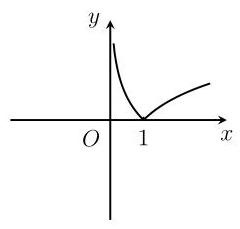
\includegraphics[max width=0.2\textwidth]{images/bo_d7fr3gc91nqc7381iccg_188_531_510_240_229_0.jpg}
\end{center}
\hspace*{3em} 

(6)

\begin{center}
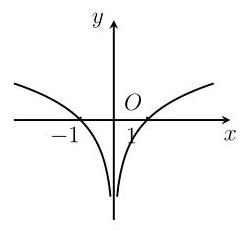
\includegraphics[max width=0.2\textwidth]{images/bo_d7fr3gc91nqc7381iccg_188_859_510_242_231_0.jpg}
\end{center}
\hspace*{3em} 

练 1 画出下列函数的图象

(1) \(y = {2}^{x + 1} - 1\) (2) \(y = {2}^{-\left| x\right| }\) (3) \(y = \left| {{2}^{\left| x\right| } - 2}\right|\)

(4) \(y = \frac{x - 1}{x + 1}\) (5) \(y = \frac{{2x} + 1}{x - 1}\) (6) \(y = \left| {x + 1}\right|\)

【答案】

\begin{center}
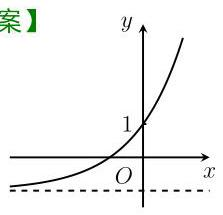
\includegraphics[max width=0.2\textwidth]{images/bo_d7fr3gc91nqc7381iccg_188_200_922_223_215_0.jpg}
\end{center}
\hspace*{3em} 

(1)

(2)

\begin{center}
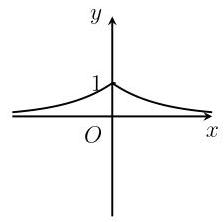
\includegraphics[max width=0.2\textwidth]{images/bo_d7fr3gc91nqc7381iccg_188_529_913_224_222_0.jpg}
\end{center}
\hspace*{3em} 

(3)

\begin{center}
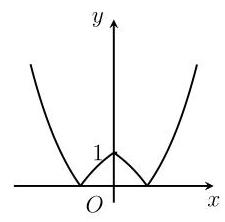
\includegraphics[max width=0.2\textwidth]{images/bo_d7fr3gc91nqc7381iccg_188_859_909_225_222_0.jpg}
\end{center}
\hspace*{3em} 

(4)

\begin{center}
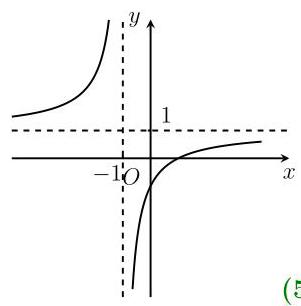
\includegraphics[max width=0.2\textwidth]{images/bo_d7fr3gc91nqc7381iccg_188_198_1150_301_306_0.jpg}
\end{center}
\hspace*{3em} 

(5)

\begin{center}
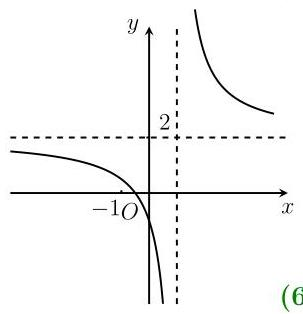
\includegraphics[max width=0.2\textwidth]{images/bo_d7fr3gc91nqc7381iccg_188_531_1143_303_314_0.jpg}
\end{center}
\hspace*{3em} 

\begin{center}
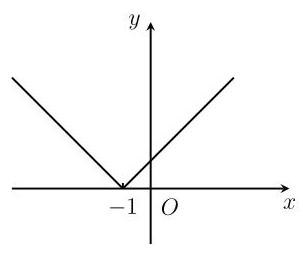
\includegraphics[max width=0.2\textwidth]{images/bo_d7fr3gc91nqc7381iccg_188_861_1203_303_253_0.jpg}
\end{center}
\hspace*{3em} 

\section*{2、根据函数的性质画图}

例 2 画出下列函数的图象

(1) \(f\left( x\right)  = x - \frac{1}{x}\)

【答案】

\begin{center}
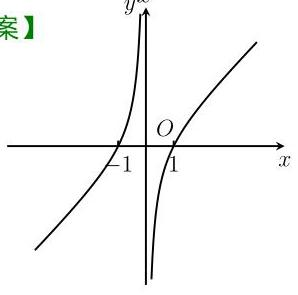
\includegraphics[max width=0.2\textwidth]{images/bo_d7fr3gc91nqc7381iccg_188_1316_229_298_295_0.jpg}
\end{center}
\hspace*{3em} 

(1)

(2) \(f\left( x\right)  = x + \ln x\)

(2)

\begin{center}
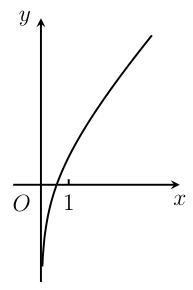
\includegraphics[max width=0.2\textwidth]{images/bo_d7fr3gc91nqc7381iccg_188_1816_232_193_290_0.jpg}
\end{center}
\hspace*{3em} 

练 2 已知奇函数 \(f\left( x\right)\) 定义域为 \(\mathbf{R}\) ,当 \(x \in  \left\lbrack  {0,1}\right\rbrack\) 时, \(f\left( x\right)  = x\) ,且 \(f\left( x\right)\) 的图象关于 \(x = 1\) 对称,画出 \(f\left( x\right)\) 在 \(\left\lbrack  {-5,5}\right\rbrack\) 的函数图象.

【答案】

\begin{center}
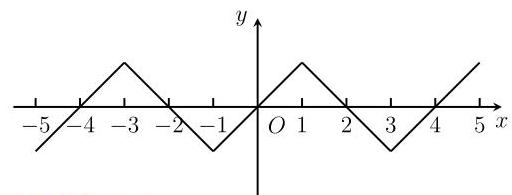
\includegraphics[max width=0.3\textwidth]{images/bo_d7fr3gc91nqc7381iccg_188_1362_670_512_195_0.jpg}
\end{center}
\hspace*{3em} 

\section*{3、复杂函数运用导数画图}

例 3 画出下列函数的图象

\begin{center}
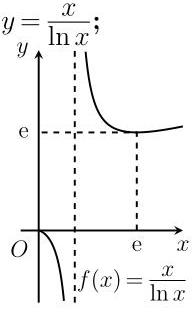
\includegraphics[max width=0.2\textwidth]{images/bo_d7fr3gc91nqc7381iccg_188_1984_972_196_313_0.jpg}
\end{center}
\hspace*{3em} 

(1) \(y = x\ln x\) (2) \(y = \frac{\ln x}{x}\) (3) \(y = \frac{x}{\ln x}\)

(1)

\begin{center}
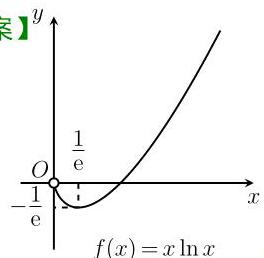
\includegraphics[max width=0.2\textwidth]{images/bo_d7fr3gc91nqc7381iccg_188_1322_1014_264_258_0.jpg}
\end{center}
\hspace*{3em} 

(2)

\begin{center}
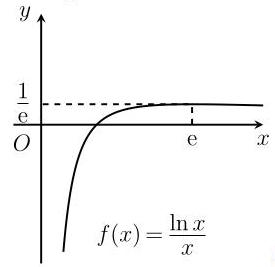
\includegraphics[max width=0.2\textwidth]{images/bo_d7fr3gc91nqc7381iccg_188_1650_1018_275_267_0.jpg}
\end{center}
\hspace*{3em} 

(3)

\section*{抛物线知识清单}

\section*{【知识清单】}

\section*{一、概念性质}

1. 定义平面内与一个定点 \(F\) 和一条定直线 \(l\left( l\right.\) 不经过点 \(\left. F\right)\) 距离相等的点的轨迹叫做抛物线. 点 \(F\) 叫做抛物线的焦点,直线 \(l\) 叫做抛物线的准线.

2.几何性质

\begin{center}
\adjustbox{max width=\textwidth}{
\begin{tabular}{|c|c|c|c|c|}
\hline
标准方程 \(\left( {p > 0}\right)\) & \({y}^{2} = {2px}\) & \({y}^{2} =  - {2px}\) & \({x}^{2} = {2py}\) & \({x}^{2} =  - {2py}\) \\
\cline{1-5}
图象 & 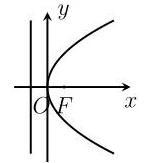
\includegraphics[max width=0.2\textwidth]{images/bo_d7fr3gc91nqc7381iccg_189_309_523_145_163_0.jpg} & 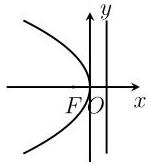
\includegraphics[max width=0.2\textwidth]{images/bo_d7fr3gc91nqc7381iccg_189_500_523_155_164_0.jpg} & 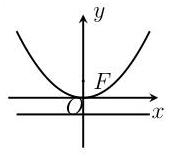
\includegraphics[max width=0.2\textwidth]{images/bo_d7fr3gc91nqc7381iccg_189_682_526_172_156_0.jpg} & 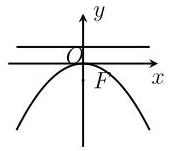
\includegraphics[max width=0.2\textwidth]{images/bo_d7fr3gc91nqc7381iccg_189_874_530_171_151_0.jpg} \\
\cline{1-5}
开口方向 & 向右 & 向左 & 向上 & 向下 \\
\cline{1-5}
焦点坐标 & \(P\left( {\frac{p}{2},0}\right)\) & \(P\left( {-\frac{p}{2},0}\right)\) & \(P\left( {0,\frac{p}{2}}\right)\) & \(P\left( {0, - \frac{p}{2}}\right)\) \\
\cline{1-5}
准线方程 & \(x =  - \frac{p}{2}\) & \(x = \frac{p}{2}\) & \(y =  - \frac{p}{2}\) & \(y = \frac{p}{2}\) \\
\cline{1-5}
对称轴 & \multicolumn{2}{|c|}{\(y = 0\)} & \multicolumn{2}{|c|}{\(x = 0\)} \\
\cline{1-5}
顶点坐标 & \multicolumn{4}{|c|}{(0,0)} \\
\cline{1-5}
离心率 & \multicolumn{4}{|c|}{\(e = 1\) (到定点与到定直线的距离之比称之为离心率)} \\
\cline{1-5}
\hline
\end{tabular}
}
\end{center}

\section*{总结记忆}

3.抛物线方程一定首先转化为标准方程;

4.焦点与一次项保持一致;

5. 焦点到原点的距离为一次项系数的 \(\frac{1}{4}\) .

\section*{二、二级结论}

1. 焦点弦 \(\left( {p > 0}\right)\)

\begin{center}
\adjustbox{max width=\textwidth}{
\begin{tabular}{|c|c|c|c|c|}
\hline
标准方程 & \({y}^{2} = {2px}\) & \({y}^{2} =  - {2px}\) & \({x}^{2} = {2py}\) & \({x}^{2} =  - {2py}\) \\
\cline{1-5}
焦点弦韦达定理 & \multicolumn{2}{|c|}{\({y}_{1}{y}_{2} = \underline{-{p}^{2}},{x}_{1}{x}_{2} = \underline{\frac{{p}^{2}}{4}}\)} & \multicolumn{2}{|c|}{\({x}_{1}{x}_{2} = \underline{-{p}^{2}},{y}_{1}{y}_{2} = \underline{\frac{{p}^{2}}{4}}\)} \\
\cline{1-5}
焦半径与坐标 & \({x}_{0} + \frac{p}{2}\) & \(- {x}_{0} + \frac{p}{2}\) & \({y}_{0} + p\) & \(- {y}_{0} + \frac{p}{2}\) \\
\cline{1-5}
焦半径与倾斜角 & \multicolumn{2}{|c|}{\(\left| {AF}\right|  = \frac{p}{1 - \cos \theta },\left| {BF}\right|  = \frac{p}{1 + \cos \theta }\) 点 \(A\) 在 \(x\) 轴上方} & \multicolumn{2}{|c|}{\(\left| {AF}\right|  = \frac{p}{1 - \sin \theta },\left| {AF}\right|  = \frac{p}{1 + \sin \theta }\) 注意焦半径小的分母较大} \\
\cline{1-5}
推论 & \multicolumn{2}{|c|}{以 \({AF}\left( {\text{ 或 }{BF}}\right)\) 为直径的圆与 \(y\) 轴相切} & \multicolumn{2}{|c|}{以 \({AF}\left( {\text{ 或 }{BF}}\right)\) 为直径的圆与 \(\underline{x}\) 轴相切} \\
\cline{1-5}
焦半径与定值 & \multicolumn{4}{|c|}{\(\frac{1}{\left| AF\right| } + \frac{1}{\left| BF\right| }\) 为定值为 \(\frac{2}{\underline{p}}\)} \\
\cline{1-5}
焦点弦长与坐标 & \({x}_{1} + {x}_{2} + p\) & \(- {x}_{1} - {x}_{2} + p\) & \({y}_{1} + {y}_{2} + p\) & \(- {y}_{1} - {y}_{2} + p\) \\
\cline{1-5}
焦点弦长与倾斜角 & \multicolumn{2}{|c|}{\(\left| {AB}\right|  = \frac{2p}{{\sin }^{2}\theta }\)} & \multicolumn{2}{|c|}{\(\left| {AB}\right|  = \frac{2p}{{\cos }^{2}\theta }\)} \\
\cline{1-5}
通径 & \multicolumn{4}{|c|}{最短的焦点弦为通径,长为 \({2p}\)} \\
\cline{1-5}
\({S}_{\bigtriangleup {OAB}}\) & \multicolumn{2}{|c|}{\(\frac{{p}^{2}}{2\sin \theta }\)} & \multicolumn{2}{|c|}{\(\frac{{p}^{2}}{2\cos \theta }\)} \\
\cline{1-5}
推论 & \multicolumn{4}{|c|}{以 \({AB}\) 为直径的圆与准线相切,记切点为 \(P\) ,则 \(\angle {APB} = {90}^{ \circ  }\)} \\
\cline{1-5}
\hline
\end{tabular}
}
\end{center}

2. 中点弦

\({y}^{2} = {2px}\) 与 \(y = {kx} + b\) 交于 \(A,B\) 两点,记 \({AB}\) 中点为 \(\left( {{x}_{0},{y}_{0}}\right)\) ,则有 \(\underline{k{y}_{0} = p}\) ;

\({x}^{2} = {2py}\) 与 \(y = {kx} + b\) 交于 \(A,B\) 两点,记 \({AB}\) 中点为 \(\left( {{x}_{0},{y}_{0}}\right)\) ,则有 \(\frac{1}{k}{x}_{0} = p\) .
\end{document}